% Options for packages loaded elsewhere
\PassOptionsToPackage{unicode}{hyperref}
\PassOptionsToPackage{hyphens}{url}
%
\documentclass[
]{book}
\usepackage{amsmath,amssymb}
\usepackage{lmodern}
\usepackage{ifxetex,ifluatex}
\ifnum 0\ifxetex 1\fi\ifluatex 1\fi=0 % if pdftex
  \usepackage[T1]{fontenc}
  \usepackage[utf8]{inputenc}
  \usepackage{textcomp} % provide euro and other symbols
\else % if luatex or xetex
  \usepackage{unicode-math}
  \defaultfontfeatures{Scale=MatchLowercase}
  \defaultfontfeatures[\rmfamily]{Ligatures=TeX,Scale=1}
\fi
% Use upquote if available, for straight quotes in verbatim environments
\IfFileExists{upquote.sty}{\usepackage{upquote}}{}
\IfFileExists{microtype.sty}{% use microtype if available
  \usepackage[]{microtype}
  \UseMicrotypeSet[protrusion]{basicmath} % disable protrusion for tt fonts
}{}
\makeatletter
\@ifundefined{KOMAClassName}{% if non-KOMA class
  \IfFileExists{parskip.sty}{%
    \usepackage{parskip}
  }{% else
    \setlength{\parindent}{0pt}
    \setlength{\parskip}{6pt plus 2pt minus 1pt}}
}{% if KOMA class
  \KOMAoptions{parskip=half}}
\makeatother
\usepackage{xcolor}
\IfFileExists{xurl.sty}{\usepackage{xurl}}{} % add URL line breaks if available
\IfFileExists{bookmark.sty}{\usepackage{bookmark}}{\usepackage{hyperref}}
\hypersetup{
  pdftitle={Simulation and Modelling to Understand Change},
  pdfauthor={Manuele Leonelli},
  hidelinks,
  pdfcreator={LaTeX via pandoc}}
\urlstyle{same} % disable monospaced font for URLs
\usepackage{color}
\usepackage{fancyvrb}
\newcommand{\VerbBar}{|}
\newcommand{\VERB}{\Verb[commandchars=\\\{\}]}
\DefineVerbatimEnvironment{Highlighting}{Verbatim}{commandchars=\\\{\}}
% Add ',fontsize=\small' for more characters per line
\usepackage{framed}
\definecolor{shadecolor}{RGB}{248,248,248}
\newenvironment{Shaded}{\begin{snugshade}}{\end{snugshade}}
\newcommand{\AlertTok}[1]{\textcolor[rgb]{0.94,0.16,0.16}{#1}}
\newcommand{\AnnotationTok}[1]{\textcolor[rgb]{0.56,0.35,0.01}{\textbf{\textit{#1}}}}
\newcommand{\AttributeTok}[1]{\textcolor[rgb]{0.77,0.63,0.00}{#1}}
\newcommand{\BaseNTok}[1]{\textcolor[rgb]{0.00,0.00,0.81}{#1}}
\newcommand{\BuiltInTok}[1]{#1}
\newcommand{\CharTok}[1]{\textcolor[rgb]{0.31,0.60,0.02}{#1}}
\newcommand{\CommentTok}[1]{\textcolor[rgb]{0.56,0.35,0.01}{\textit{#1}}}
\newcommand{\CommentVarTok}[1]{\textcolor[rgb]{0.56,0.35,0.01}{\textbf{\textit{#1}}}}
\newcommand{\ConstantTok}[1]{\textcolor[rgb]{0.00,0.00,0.00}{#1}}
\newcommand{\ControlFlowTok}[1]{\textcolor[rgb]{0.13,0.29,0.53}{\textbf{#1}}}
\newcommand{\DataTypeTok}[1]{\textcolor[rgb]{0.13,0.29,0.53}{#1}}
\newcommand{\DecValTok}[1]{\textcolor[rgb]{0.00,0.00,0.81}{#1}}
\newcommand{\DocumentationTok}[1]{\textcolor[rgb]{0.56,0.35,0.01}{\textbf{\textit{#1}}}}
\newcommand{\ErrorTok}[1]{\textcolor[rgb]{0.64,0.00,0.00}{\textbf{#1}}}
\newcommand{\ExtensionTok}[1]{#1}
\newcommand{\FloatTok}[1]{\textcolor[rgb]{0.00,0.00,0.81}{#1}}
\newcommand{\FunctionTok}[1]{\textcolor[rgb]{0.00,0.00,0.00}{#1}}
\newcommand{\ImportTok}[1]{#1}
\newcommand{\InformationTok}[1]{\textcolor[rgb]{0.56,0.35,0.01}{\textbf{\textit{#1}}}}
\newcommand{\KeywordTok}[1]{\textcolor[rgb]{0.13,0.29,0.53}{\textbf{#1}}}
\newcommand{\NormalTok}[1]{#1}
\newcommand{\OperatorTok}[1]{\textcolor[rgb]{0.81,0.36,0.00}{\textbf{#1}}}
\newcommand{\OtherTok}[1]{\textcolor[rgb]{0.56,0.35,0.01}{#1}}
\newcommand{\PreprocessorTok}[1]{\textcolor[rgb]{0.56,0.35,0.01}{\textit{#1}}}
\newcommand{\RegionMarkerTok}[1]{#1}
\newcommand{\SpecialCharTok}[1]{\textcolor[rgb]{0.00,0.00,0.00}{#1}}
\newcommand{\SpecialStringTok}[1]{\textcolor[rgb]{0.31,0.60,0.02}{#1}}
\newcommand{\StringTok}[1]{\textcolor[rgb]{0.31,0.60,0.02}{#1}}
\newcommand{\VariableTok}[1]{\textcolor[rgb]{0.00,0.00,0.00}{#1}}
\newcommand{\VerbatimStringTok}[1]{\textcolor[rgb]{0.31,0.60,0.02}{#1}}
\newcommand{\WarningTok}[1]{\textcolor[rgb]{0.56,0.35,0.01}{\textbf{\textit{#1}}}}
\usepackage{longtable,booktabs,array}
\usepackage{calc} % for calculating minipage widths
% Correct order of tables after \paragraph or \subparagraph
\usepackage{etoolbox}
\makeatletter
\patchcmd\longtable{\par}{\if@noskipsec\mbox{}\fi\par}{}{}
\makeatother
% Allow footnotes in longtable head/foot
\IfFileExists{footnotehyper.sty}{\usepackage{footnotehyper}}{\usepackage{footnote}}
\makesavenoteenv{longtable}
\usepackage{graphicx}
\makeatletter
\def\maxwidth{\ifdim\Gin@nat@width>\linewidth\linewidth\else\Gin@nat@width\fi}
\def\maxheight{\ifdim\Gin@nat@height>\textheight\textheight\else\Gin@nat@height\fi}
\makeatother
% Scale images if necessary, so that they will not overflow the page
% margins by default, and it is still possible to overwrite the defaults
% using explicit options in \includegraphics[width, height, ...]{}
\setkeys{Gin}{width=\maxwidth,height=\maxheight,keepaspectratio}
% Set default figure placement to htbp
\makeatletter
\def\fps@figure{htbp}
\makeatother
\setlength{\emergencystretch}{3em} % prevent overfull lines
\providecommand{\tightlist}{%
  \setlength{\itemsep}{0pt}\setlength{\parskip}{0pt}}
\setcounter{secnumdepth}{5}
\usepackage{booktabs}
\ifluatex
  \usepackage{selnolig}  % disable illegal ligatures
\fi
\usepackage[]{natbib}
\bibliographystyle{apalike}

\title{Simulation and Modelling to Understand Change}
\author{Manuele Leonelli}
\date{2021-04-19}

\begin{document}
\maketitle

{
\setcounter{tocdepth}{1}
\tableofcontents
}
\hypertarget{preface}{%
\chapter*{Preface}\label{preface}}
\addcontentsline{toc}{chapter}{Preface}

These are lecture notes for the module \emph{Simulation and Modelling to Understand Change} given in the School of Human Sciences and Technology at IE University, Madrid, Spain. The module is given in the 2nd semester of the 1st year of the bachelor in Data \& Business Analytics. Knowledge of basic elements of R programming as well as probability and statistics is assumed.

\hypertarget{intro}{%
\chapter{Introduction}\label{intro}}

The first introductory chapter gives an overview of simulation, what it is, what it can be used for, as well as some examples.

\hypertarget{what-is-simulation}{%
\section{What is simulation}\label{what-is-simulation}}

A \emph{simulation} is an imitation of the dynamics of a real-world process or system over time. Although simulation could potentially still be done ``by hand'', nowadays it almost always implicitly requires the use of a computer to create an artificial history of a system to draw inferences about its characteristics and workings.

The behavior of the system is studied by constructing a \emph{simulation model}, which usually takes the form of a set of assumptions about the workings of the system. Once developed, a simulation model can be used for a variety of tasks, including:

\begin{itemize}
\item
  Investigate the behaviour of the system under a wide array of scenarios. This is also often referred to as ``what-if'' analyses;
\item
  Changes to the system can be simulated before implementation to predict their impact in real-world;
\item
  During the design stage of a system, meaning while it is being built, simulation can be used to guide its construction.
\end{itemize}

Computer simulation has been used in a variety of domains, including manifacturing, health care, transport system, defense and management science, among many others.

\hypertarget{a-simple-simulation-model}{%
\subsection{A simple simulation model}\label{a-simple-simulation-model}}

Suppose we decided to open a donut shop and are unsure about how many employees to hire to sell donuts to costumers. The operations of our little shop is the real-world system whose behavior we want to understand. Given that the shop is not operating yet, only a simulation model can provide us with insights.

We could of course devise models of different complexities, but for now suppose that we are happy with a simple model where we have the following elements:

\begin{itemize}
\item
  costumers that arrive at our shop at a particular rate;
\item
  employees (of a number to be given as input) that take a specific time to serve costumers.
\end{itemize}

Implicitly, we are completely disregarding the number of donuts available in our shop and assuming that we have an infinite availability of these. Of course, in a more complex simulation model we may want to also include this element to give a more realistic description of the system.

\hypertarget{why-simulate}{%
\subsection{Why simulate?}\label{why-simulate}}

An alternative approach to computer simulation is direct experimentation. In the bagel shop setting, we could wait for the shop to open and observe its workings by having a different number of employees on different days. Considered against real experimentation, simulation has the following advantages:

\begin{itemize}
\item
  It is \emph{cheaper} to implement and does not require a disruption of the real-world system;
\item
  It is \emph{faster} to implement and time can be compressed or expanded to allow for a speed-up or a slow-down of the system of interest;
\item
  It can be \emph{replicated} multiple times and the workings of the systems can be observed a large number of times;
\item
  It is \emph{safe} since it does not require an actual disruption of the system;
\item
  It is \emph{ethical} and \emph{legal} since it can implement changes in policies that would be unethical or illegal to do in real-world.
\end{itemize}

Another alternative is to use a mathematical model representing the system. However, it is often infeasible, if not impossible, to come up with an exact mathematical model which can faithfully represent the system under study.

\hypertarget{types-of-simulations}{%
\section{Types of simulations}\label{types-of-simulations}}

Before starting the construction of a simulation model, we need to decide upon the principal characteristics of that model. There are various choices to be made, which depend upon the system we are trying to understand.

\hypertarget{stochastic-vs-deterministic-simulations}{%
\subsection{Stochastic vs deterministic simulations}\label{stochastic-vs-deterministic-simulations}}

A model is \emph{deterministic} if its behavior is entirely predictable. Given a set of inputs, the model will result in a unique set of outputs. A model is \emph{stochastic} if it has random variables as inputs, and consequently also its outputs are random.

Consider the donut shop example. In a deterministic model we would for instance assume that a new customer arrives every 5 minutes and an employee takes 2 minutes to serve a customer. In a stochastic model we would on the other hand assume that the arrival times and the serving time follows some random variables: for instance, normal distributions with some mean and variance parameters.

In this course we will only consider stochastic simulation, but for illustration we consider now an example of a deterministic simulation.

A social media influencer decides to open a new page and her target is to reach 10k followers in 10 weeks. Given her past experience, she assumes that each week she will get 1.5k new followers that had never followed the page and of her current followers she believes 10\% will stop following the page each week. However, 20\% of those that the left the page in the past will join again each week. Will she reach her target?

To answer this question we can construct a deterministic simulation. Let \(F_t\) the number of followers at week \(t\) and \(U_t\) the number of users that are unfollowing the profile at week \(t\). Then
\[
F_t = F_{t-1} + 1500 - L_{t} + R_{t}, \hspace{1cm} U_t= U_{t-1} + L_{t} - R_{t}
\]
where \(L_{t}=0.1\cdot F_{t-1}\) is the number of unfollowers from time \(t-1\) to time \(t\), and \(R_{t}=0.2\cdot U_{t-1}\) is the number of users that follow the page back from time \(t-1\) to time \(t\).

To compute the number of followers after ten weeks we can use the R code below. It does not matter if you do not understand it now, we will review R coding in the next chapters.

\begin{Shaded}
\begin{Highlighting}[]
\NormalTok{Ft }\OtherTok{\textless{}{-}}\NormalTok{ Ut }\OtherTok{\textless{}{-}}\NormalTok{ Lt }\OtherTok{\textless{}{-}}\NormalTok{ Rt }\OtherTok{\textless{}{-}} \FunctionTok{rep}\NormalTok{(}\DecValTok{0}\NormalTok{,}\DecValTok{11}\NormalTok{)}
\ControlFlowTok{for}\NormalTok{ (i }\ControlFlowTok{in} \DecValTok{2}\SpecialCharTok{:}\DecValTok{11}\NormalTok{)\{}
\NormalTok{  Lt[i] }\OtherTok{\textless{}{-}} \FloatTok{0.1}\SpecialCharTok{*}\NormalTok{Ft[i}\DecValTok{{-}1}\NormalTok{]}
\NormalTok{  Rt[i] }\OtherTok{\textless{}{-}} \FloatTok{0.2}\SpecialCharTok{*}\NormalTok{Ut[i}\DecValTok{{-}1}\NormalTok{]}
\NormalTok{  Ut[i] }\OtherTok{\textless{}{-}}\NormalTok{ Ut[i}\DecValTok{{-}1}\NormalTok{] }\SpecialCharTok{+}\NormalTok{ Lt[i] }\SpecialCharTok{{-}}\NormalTok{ Rt[i]}
\NormalTok{  Ft[i] }\OtherTok{\textless{}{-}}\NormalTok{ Ft[i}\DecValTok{{-}1}\NormalTok{] }\SpecialCharTok{+} \DecValTok{1500} \SpecialCharTok{{-}}\NormalTok{ Lt[i] }\SpecialCharTok{+}\NormalTok{ Rt[i]}
\NormalTok{\}}
\NormalTok{result }\OtherTok{\textless{}{-}} \FunctionTok{data.frame}\NormalTok{(}\StringTok{"Followers"} \OtherTok{=}\NormalTok{ Ft, }\StringTok{"Total Unfollowers"} \OtherTok{=}\NormalTok{ Ut,}
           \StringTok{"Weekly Unfollowers"} \OtherTok{=}\NormalTok{ Ut, }\StringTok{"Weekly Returns"} \OtherTok{=}\NormalTok{ Rt)}
\end{Highlighting}
\end{Shaded}

The dataframe \texttt{result} is reported in Table \ref{tab:insta}, showing that she will be able to hit her target of 10k followers since she will have 11619 followers. If we run again the simulation we will obtain the exact same results: there is no stochasticity/uncertainty about the outcome.

\begin{table}

\caption{\label{tab:insta}Dataframe `result` from the social media deterministic simulation}
\centering
\begin{tabular}[t]{rrrr}
\toprule
Followers & Total.Unfollowers & Weekly.Unfollowers & Weekly.Returns\\
\midrule
0.000 & 0.000 & 0.000 & 0.0000\\
1500.000 & 0.000 & 0.000 & 0.0000\\
2850.000 & 150.000 & 150.000 & 0.0000\\
4095.000 & 405.000 & 405.000 & 30.0000\\
5266.500 & 733.500 & 733.500 & 81.0000\\
\addlinespace
6386.550 & 1113.450 & 1113.450 & 146.7000\\
7470.585 & 1529.415 & 1529.415 & 222.6900\\
8529.409 & 1970.591 & 1970.591 & 305.8830\\
9570.587 & 2429.413 & 2429.413 & 394.1181\\
10599.411 & 2900.589 & 2900.589 & 485.8827\\
\addlinespace
11619.587 & 3380.413 & 3380.413 & 580.1179\\
\bottomrule
\end{tabular}
\end{table}

The above application could be transformed into a stochastic simulation by allowing the rate at which she gets new followers, unfollowers etc. to be random variables of which we do not know the exact value.

\hypertarget{static-vs-dynamic-simulations}{%
\subsection{Static vs dynamic simulations}\label{static-vs-dynamic-simulations}}

Simulation models that represent the system at a particular point in time only are called \emph{static}. This type of simulations are often called as \emph{Monte Carlo simulations} and will be the focus of later chapters.

\emph{Dynamic} simulation models represent systems as they evolve over time. The simulation of the donut shop during its working hours is an example of a dynamic model.

\hypertarget{discrete-vs-continuous-simulations}{%
\subsection{Discrete vs continuous simulations}\label{discrete-vs-continuous-simulations}}

Dynamic simulations can be further categorized into discrete or continuous.

\emph{Discrete} simulation models are such that the variables of interest change only at a discrete set of points in time. The number of people queuing in the donut shop is an example of a discrete simulation. The number of customers changes only when a new customer arrives or when a customer has been served. Figure 1.1 gives an illustration of the discrete nature of the number of customers queuing in the donut shop.

\begin{figure}

{\centering 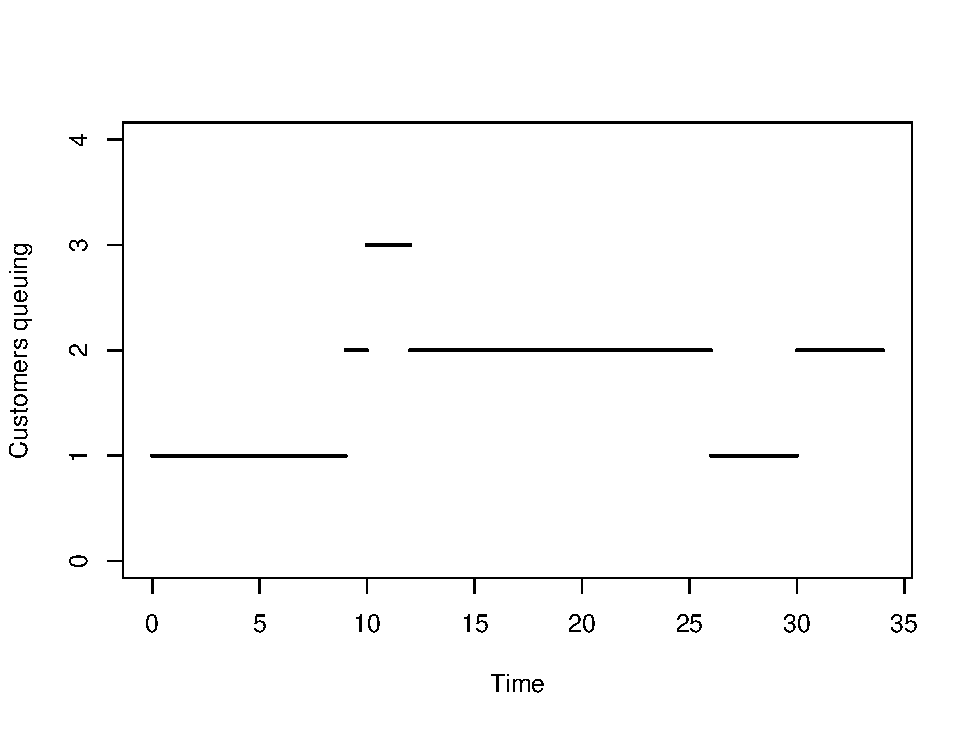
\includegraphics[width=0.8\linewidth]{SimBook_files/figure-latex/discrete-1} 

}

\caption{Example of a discrete dynamic simulation}\label{fig:discrete}
\end{figure}

Figure 1.1 further illustrates that for specific period of times the system does not change state, that is the number of customers queuing remains constant. It is therefore useless to inspect the system during those times where nothing changes. This prompts the way in which time is usually handled in dynamic discrete simulations, using the so-called \emph{next-event technique}. The model is only examined and updated when the system is due to change. These changes are usually called \emph{events}. Looking at Figure 1.1 at time zero there is an event: a customer arrives; at time nine another customer arrives; at time ten another customer arrives; at time twelve a customer is served; and so on. All these are examples of events.

\emph{Continuous} simulation models are such that the variables of interest change continuously over time. Suppose for instance a simulation model for a car journey was created where the interest is on the speed of the car throughout the journey. Then this would be a continuous simulation model. Figure 1.2 gives an illustration of this.

\begin{figure}

{\centering 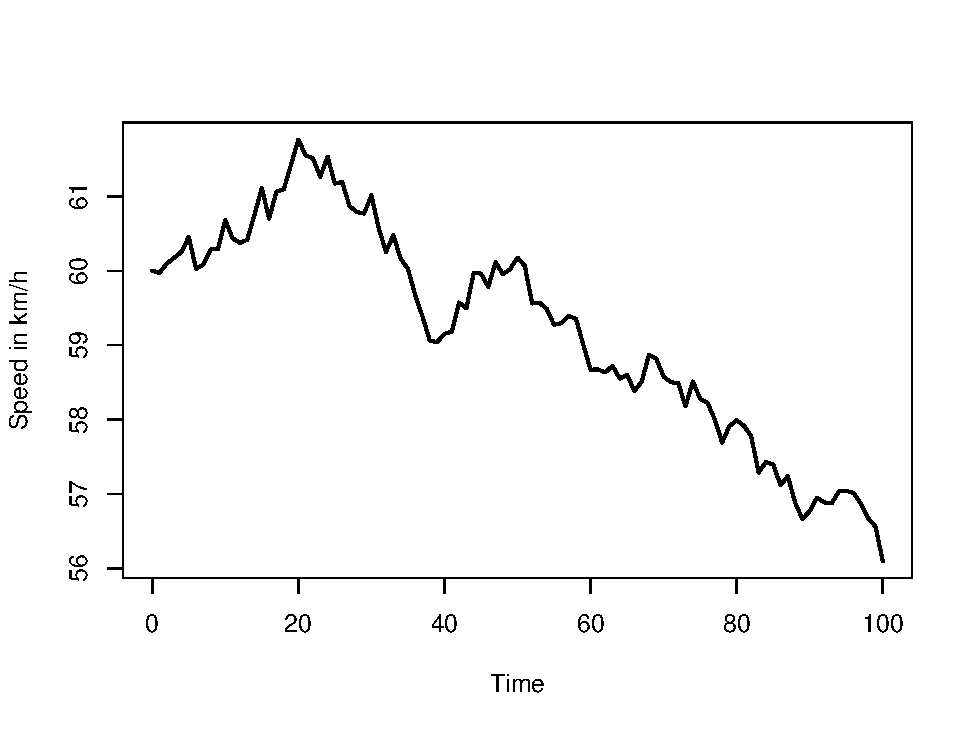
\includegraphics[width=0.8\linewidth]{SimBook_files/figure-latex/fig-cont-1} 

}

\caption{Example of a discrete dynamic simulation}\label{fig:fig-cont}
\end{figure}

In later chapters we will focus on discrete simulations, which are usually called \emph{discrete-event simulation}. Continuous simulations will not be discussed in these notes.

\hypertarget{elements-of-a-simulation-model}{%
\section{Elements of a simulation model}\label{elements-of-a-simulation-model}}

We next introduce some terminology which we will need in the following.

\hypertarget{objects-of-the-model}{%
\subsection{Objects of the model}\label{objects-of-the-model}}

There are two types of objects a simulation model is often made of:

\begin{itemize}
\item
  \emph{Entities}: individual elements of the system that are being simulated and whose behavior is being explicitly tracked. Each entity can be individually identified;
\item
  \emph{Resources}: also individual elements of the system but they are not modelled individually. They are treated as countable items whose behavior is not tracked.
\end{itemize}

Whether an element should be treated as an entity or as a resource is something that the modeller must decide and depends on the purpose of the simulation. Consider our simple donut shop. Clients will be most likely be resources since we are not really interested in what each of them do. Employees may either be considered as entities or resources: in the former case we want to track the amount of time each of them are working; in the latter the model would only be able to output an overview of how busy overall the employees are.

\hypertarget{organization-of-entities-and-resources}{%
\subsection{Organization of entities and resources}\label{organization-of-entities-and-resources}}

\begin{itemize}
\item
  \emph{Attributes}: properties of objects (that is entities and resources). This is often used to control the behavior of the object. In our donut shop an attribute may be the state of an employee: whether she is busy or available. In a more comprehensive simulation, an attribute might be the type of donut a customer will buy (for instance, chocolate, vanilla or jam).
\item
  \emph{State}: collection of variables necessary to describe the system at any time point. In our donut shop, in the simplest case the necessary variables are number of customers queuing and number of busy employees. This fully characterizes the system.
\item
  \emph{List}: collection of entites or resources ordered in some logical fashion. For instance, the customers waiting in our shop may be ordered in the so-called ``fist-come, first-served" scheme, that is customers will be served in the order they arrived in the shop.
\end{itemize}

\hypertarget{operations-of-the-objects}{%
\subsection{Operations of the objects}\label{operations-of-the-objects}}

During a simulation study, entities and resources will cooperate and therefore change state. The following terminology describe this as well as the flow of time:

\begin{itemize}
\item
  \emph{Event}: instant of time where the state of the system changes. In the donut shop suppose that there are currently two customers being served. An event is when a customer has finished being served: the number of busy employees decreases by one and there is one less customer queuing.
\item
  \emph{Activity}: a time period of specified length which is known when it begins (although its length may be random). The time an employee takes to serve a customer is an example of an activity: this may be specified in terms of a random distribution.
\item
  \emph{Delay}: duration of time of unspecified length, which is not known until it ends. This is not specified by the modeller ahead of time but is determined by the conditions of the system. Very often this is one of the desired output of a simulation. For instance, a delay is the waiting time of a customer in the queue of our donut shop.
\item
  \emph{Clock}: variable representing simulated time.
\end{itemize}

\hypertarget{the-donut-shop-example}{%
\section{The donut shop example}\label{the-donut-shop-example}}

Let's consider in more details the donut shop example and let's construct and implement our first simulation model. At this stage, you should not worry about the implementation details. These will be formalized in more details in later chapters.

Let's make some assumptions:

\begin{itemize}
\item
  the queue in the shop is possibly infinite: whenever a customer arrives she will stay in the queue independent of how many customers are already queuing and she will wait until she is served.
\item
  customers are served on a first-come, first-served basis.
\item
  there are two employees. On average they take the same time to serve a customer. Whenever an employee is free, a customer is allocated to that employee. If both employees are free, either of the two starts serving a customer.
\end{itemize}

The components of the simulation model are the following:

\begin{itemize}
\item
  \textbf{System state}: \(N_C(t)\) number of customers waiting to be served at time \(t\); \(N_E(t)\) number of employees busy at time \(t\).
\item
  \textbf{Resources}: customers and employees;
\item
  \textbf{Events}: arrival of a customer; service completion by an employee.
\item
  \textbf{Activities}: time between a customer arrival and the next; service time by an employee.
\item
  \textbf{Delay}: customers' waiting time in the queue until an employee is available.
\end{itemize}

From an abstract point of view we have now defined all components of our simulation model. Before implementing, we need to choose the length of the activities. This is usually done using common sense, intuition or historical data. Suppose for instance that the time between the arrival of customers is modeled as an Exponential distribution with parameter 1/3 (that is on average a customer arrives every three minutes) and the service time is modeled as a continuous Uniform distribution between 1 and 5 (on average a service takes three minutes).

With this information we can now implement the workings of our donut shop. It does not matter the specific code itself, we will learn about it in later chapters. At this stage it is only important to notice that we use the \texttt{simmer} package together with the functionalities of \texttt{magrittr}. We simulate our donut shop for two hours.

\begin{Shaded}
\begin{Highlighting}[]
\FunctionTok{library}\NormalTok{(simmer)}
\FunctionTok{library}\NormalTok{(magrittr)}
\FunctionTok{set.seed}\NormalTok{(}\DecValTok{2021}\NormalTok{)}

\NormalTok{env }\OtherTok{\textless{}{-}}  \FunctionTok{simmer}\NormalTok{(}\StringTok{"donut shop"}\NormalTok{)}

\NormalTok{customer }\OtherTok{\textless{}{-}} \FunctionTok{trajectory}\NormalTok{(}\StringTok{"customer"}\NormalTok{) }\SpecialCharTok{\%\textgreater{}\%} \FunctionTok{seize}\NormalTok{(}\StringTok{"employee"}\NormalTok{, }\DecValTok{1}\NormalTok{) }\SpecialCharTok{\%\textgreater{}\%}
  \FunctionTok{timeout}\NormalTok{(}\ControlFlowTok{function}\NormalTok{() }\FunctionTok{runif}\NormalTok{(}\DecValTok{1}\NormalTok{,}\DecValTok{1}\NormalTok{,}\DecValTok{5}\NormalTok{)) }\SpecialCharTok{\%\textgreater{}\%} \FunctionTok{release}\NormalTok{(}\StringTok{"employee"}\NormalTok{, }\DecValTok{1}\NormalTok{) }

\NormalTok{env }\SpecialCharTok{\%\textgreater{}\%}
  \FunctionTok{add\_resource}\NormalTok{(}\StringTok{"employee"}\NormalTok{, }\DecValTok{2}\NormalTok{) }\SpecialCharTok{\%\textgreater{}\%}
  \FunctionTok{add\_generator}\NormalTok{(}\StringTok{"customer"}\NormalTok{, customer, }\ControlFlowTok{function}\NormalTok{() }\FunctionTok{rexp}\NormalTok{(}\DecValTok{1}\NormalTok{,}\DecValTok{1}\SpecialCharTok{/}\DecValTok{3}\NormalTok{))}

\NormalTok{env }\SpecialCharTok{\%\textgreater{}\%}
  \FunctionTok{run}\NormalTok{(}\AttributeTok{until=}\DecValTok{120}\NormalTok{)}
\end{Highlighting}
\end{Shaded}

The above code creates a simulation of the donut shop for two hours. Next we report some graphical summaries that describe how the system worked.

\begin{Shaded}
\begin{Highlighting}[]
\FunctionTok{library}\NormalTok{(simmer.plot)}
\FunctionTok{library}\NormalTok{(gridExtra)}
\NormalTok{p1 }\OtherTok{\textless{}{-}} \FunctionTok{plot}\NormalTok{(}\FunctionTok{get\_mon\_resources}\NormalTok{(env), }\AttributeTok{metric =} \StringTok{"usage"}\NormalTok{, }\AttributeTok{items =} \StringTok{"server"}\NormalTok{,}\AttributeTok{step =}\NormalTok{ T)}
\NormalTok{p2 }\OtherTok{\textless{}{-}} \FunctionTok{plot}\NormalTok{(}\FunctionTok{get\_mon\_arrivals}\NormalTok{(env), }\AttributeTok{metric =} \StringTok{"waiting\_time"}\NormalTok{)}

\FunctionTok{grid.arrange}\NormalTok{(p1,p2,}\AttributeTok{ncol=}\DecValTok{2}\NormalTok{)}
\end{Highlighting}
\end{Shaded}

\begin{figure}

{\centering 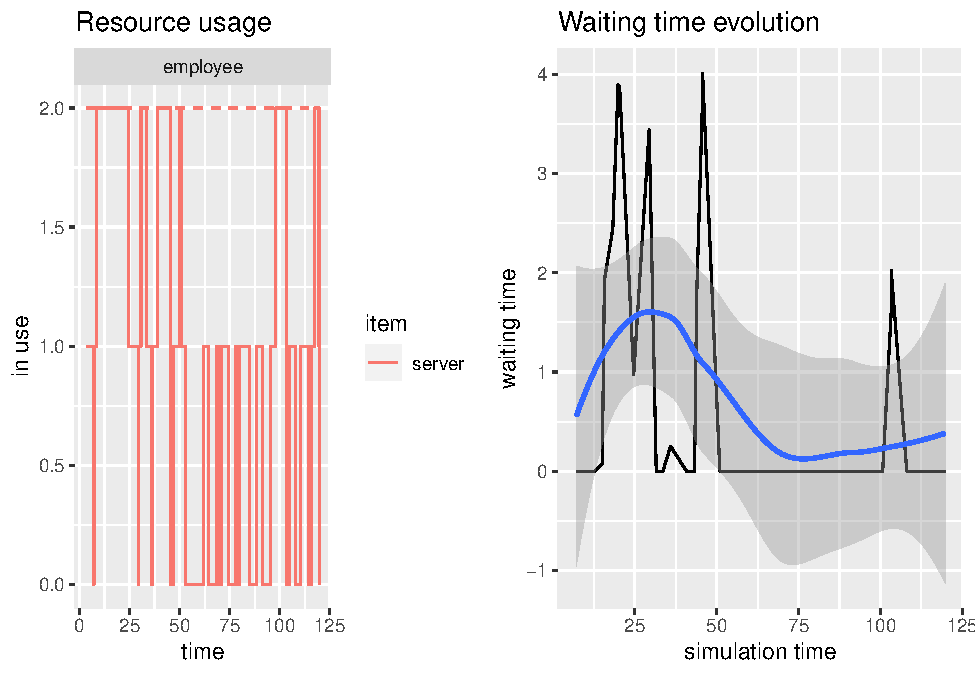
\includegraphics{SimBook_files/figure-latex/donut-1} 

}

\caption{Graphical summaries from the simulation of the donut shop}\label{fig:donut}
\end{figure}

The left plot in Figure 1.3 reports the number of busy employees busy throughout the simulation. We can observe that often no employees were busy, but sometimes both of them are busy. The right plot in Figure 1.3 reports the waiting time of customers throughout the simulation. Most often customers do not wait in our shop and the largest waiting time is of about four minutes.

Some observations:

\begin{itemize}
\item
  this is the result of a single simulation where inputs are random and described by a random variable (for instance, Poisson and Uniform). If we were to run the simulation again we would observe different results.
\item
  given that we have built the simulation model, it is straightforward to change some of the inputs and observe the results under different conditions. For instance, we could investigate what would happen if we had only one employee. We could also investigate the use of different input parameters for the customer arrival times and the service times.
\end{itemize}

\hypertarget{simulating-a-little-health-center}{%
\section{Simulating a little health center}\label{simulating-a-little-health-center}}

Consider now a slightly more complex example where we want to simulate the workings of a little health center. Patients arrive at the health center and are first visited by a nurse. Once they are visited by the nurse they have an actual consultation with a doctor. Once they are finished with the doctor, they meet the administrative staff to schedule a follow-up appointment.

We make the following assumptions:

\begin{itemize}
\item
  as before we assume queues to be infinite and that patients do not leave the health center until they are served by the administrative staff;
\item
  at all steps patients are visited using a first-come, first-served basis
\item
  the health center has one nurse, two doctors and one administrative staff. The two doctors take on average the same time to visit a patient.
\end{itemize}

The components of the simulation model are the following:

\begin{itemize}
\item
  \textbf{System state}:

  \begin{itemize}
  \item
    \(Q_N(t)\): number of patients queuing to see the nurse;
  \item
    \(Q_D(t)\): number of patients queing to see a doctor;
  \item
    \(Q_A(t)\): number of patients queuing to see the staff;
  \item
    \(N_N(t)\): number of nurses available to visit patients;
  \item
    \(N_D(t)\): number of doctors available to visit patients;
  \item
    \(N_A(t)\): number of administrative staff available to visit patients.
  \end{itemize}
\item
  \textbf{Resources}: patients, nurses, doctors and administrative staff;
\item
  \textbf{Events}: arrival of a patient, completion of nurse's visit, completation of doctor's visit, completion of administrative staff's visit.
\item
  \textbf{Activities}: time between the arrival of a patient and the next, visit's times of nurses, doctors and admin staff.
\item
  \textbf{Delay}: customers' waiting time for nurses, doctors and administrative staff
\end{itemize}

We further assume the following activities:

\begin{itemize}
\item
  Nurse visit times follow a Normal distribution with mean 15 and variance 1;
\item
  Doctor visit times follow a Normal distribution with mean 20 and variance 1;
\item
  Administrative staff visit times follow a Normal distribution with mean 5 and variance 1;
\item
  Time between the arrival of patients is modeled as a Normal with mean 10 and variance 4.
\end{itemize}

The model above can be implemented using the following code (we run the simulation for four hours). Again do not worry about it now!

\begin{Shaded}
\begin{Highlighting}[]
\FunctionTok{set.seed}\NormalTok{(}\DecValTok{2021}\NormalTok{)}
\NormalTok{env }\OtherTok{\textless{}{-}} \FunctionTok{simmer}\NormalTok{(}\StringTok{"HealthCenter"}\NormalTok{)}

\NormalTok{patient }\OtherTok{\textless{}{-}} \FunctionTok{trajectory}\NormalTok{(}\StringTok{"patients\textquotesingle{} path"}\NormalTok{) }\SpecialCharTok{\%\textgreater{}\%}
  \FunctionTok{seize}\NormalTok{(}\StringTok{"nurse"}\NormalTok{, }\DecValTok{1}\NormalTok{) }\SpecialCharTok{\%\textgreater{}\%}
  \FunctionTok{timeout}\NormalTok{(}\ControlFlowTok{function}\NormalTok{() }\FunctionTok{rnorm}\NormalTok{(}\DecValTok{1}\NormalTok{, }\DecValTok{15}\NormalTok{)) }\SpecialCharTok{\%\textgreater{}\%}
  \FunctionTok{release}\NormalTok{(}\StringTok{"nurse"}\NormalTok{, }\DecValTok{1}\NormalTok{) }\SpecialCharTok{\%\textgreater{}\%}
  \FunctionTok{seize}\NormalTok{(}\StringTok{"doctor"}\NormalTok{, }\DecValTok{1}\NormalTok{) }\SpecialCharTok{\%\textgreater{}\%}
  \FunctionTok{timeout}\NormalTok{(}\ControlFlowTok{function}\NormalTok{() }\FunctionTok{rnorm}\NormalTok{(}\DecValTok{1}\NormalTok{, }\DecValTok{20}\NormalTok{)) }\SpecialCharTok{\%\textgreater{}\%}
  \FunctionTok{release}\NormalTok{(}\StringTok{"doctor"}\NormalTok{, }\DecValTok{1}\NormalTok{) }\SpecialCharTok{\%\textgreater{}\%}
  \FunctionTok{seize}\NormalTok{(}\StringTok{"administration"}\NormalTok{, }\DecValTok{1}\NormalTok{) }\SpecialCharTok{\%\textgreater{}\%}
  \FunctionTok{timeout}\NormalTok{(}\ControlFlowTok{function}\NormalTok{() }\FunctionTok{rnorm}\NormalTok{(}\DecValTok{1}\NormalTok{, }\DecValTok{5}\NormalTok{)) }\SpecialCharTok{\%\textgreater{}\%}
  \FunctionTok{release}\NormalTok{(}\StringTok{"administration"}\NormalTok{, }\DecValTok{1}\NormalTok{)}

\NormalTok{env }\SpecialCharTok{\%\textgreater{}\%}
  \FunctionTok{add\_resource}\NormalTok{(}\StringTok{"nurse"}\NormalTok{, }\DecValTok{1}\NormalTok{) }\SpecialCharTok{\%\textgreater{}\%}
  \FunctionTok{add\_resource}\NormalTok{(}\StringTok{"doctor"}\NormalTok{, }\DecValTok{2}\NormalTok{) }\SpecialCharTok{\%\textgreater{}\%}
  \FunctionTok{add\_resource}\NormalTok{(}\StringTok{"administration"}\NormalTok{, }\DecValTok{1}\NormalTok{) }\SpecialCharTok{\%\textgreater{}\%}
  \FunctionTok{add\_generator}\NormalTok{(}\StringTok{"patient"}\NormalTok{, patient, }\ControlFlowTok{function}\NormalTok{() }\FunctionTok{rnorm}\NormalTok{(}\DecValTok{1}\NormalTok{, }\DecValTok{10}\NormalTok{, }\DecValTok{2}\NormalTok{))}

\NormalTok{env }\SpecialCharTok{\%\textgreater{}\%} \FunctionTok{run}\NormalTok{(}\DecValTok{240}\NormalTok{)}
\end{Highlighting}
\end{Shaded}

Let's look at some summary statistics.

\begin{Shaded}
\begin{Highlighting}[]
\FunctionTok{plot}\NormalTok{(}\FunctionTok{get\_mon\_resources}\NormalTok{(env), }\AttributeTok{metric =} \StringTok{"utilization"}\NormalTok{)}
\end{Highlighting}
\end{Shaded}

\begin{figure}

{\centering 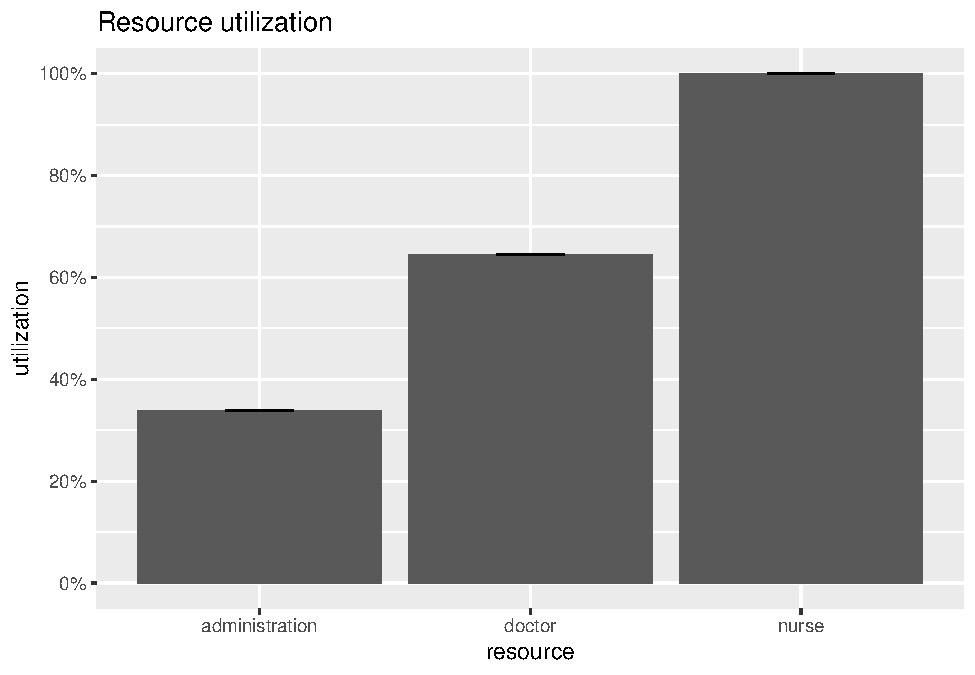
\includegraphics{SimBook_files/figure-latex/unnamed-chunk-4-1} 

}

\caption{Utilization of the resources in the health center}\label{fig:unnamed-chunk-4}
\end{figure}

Figure 1.4 shows the utilization of the different resources in the system. Nurses are most busy, doctors are overall fairly available, whilst the administration is more than half of the time available.

\begin{Shaded}
\begin{Highlighting}[]
\FunctionTok{plot}\NormalTok{(}\FunctionTok{get\_mon\_resources}\NormalTok{(env), }\AttributeTok{metric =} \StringTok{"usage"}\NormalTok{, }\AttributeTok{item =} \StringTok{"server"}\NormalTok{)}
\end{Highlighting}
\end{Shaded}

\begin{figure}

{\centering 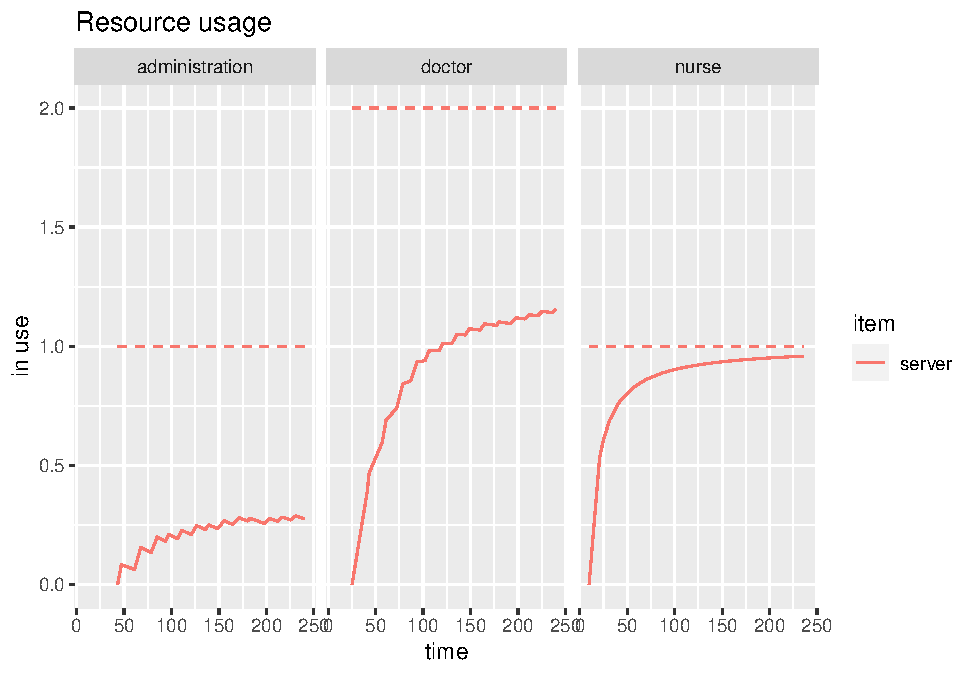
\includegraphics{SimBook_files/figure-latex/unnamed-chunk-5-1} 

}

\caption{Usage of the resources in the health center}\label{fig:unnamed-chunk-5}
\end{figure}

Figure 1.5 confirms this. We see that the usage of nurses is almost 1, whilst for doctors and administrative staff we are below the number of doctors and staff available.

\begin{Shaded}
\begin{Highlighting}[]
\FunctionTok{plot}\NormalTok{(}\FunctionTok{get\_mon\_arrivals}\NormalTok{(env), }\AttributeTok{metric =} \StringTok{"flow\_time"}\NormalTok{)}
\end{Highlighting}
\end{Shaded}

\begin{figure}

{\centering 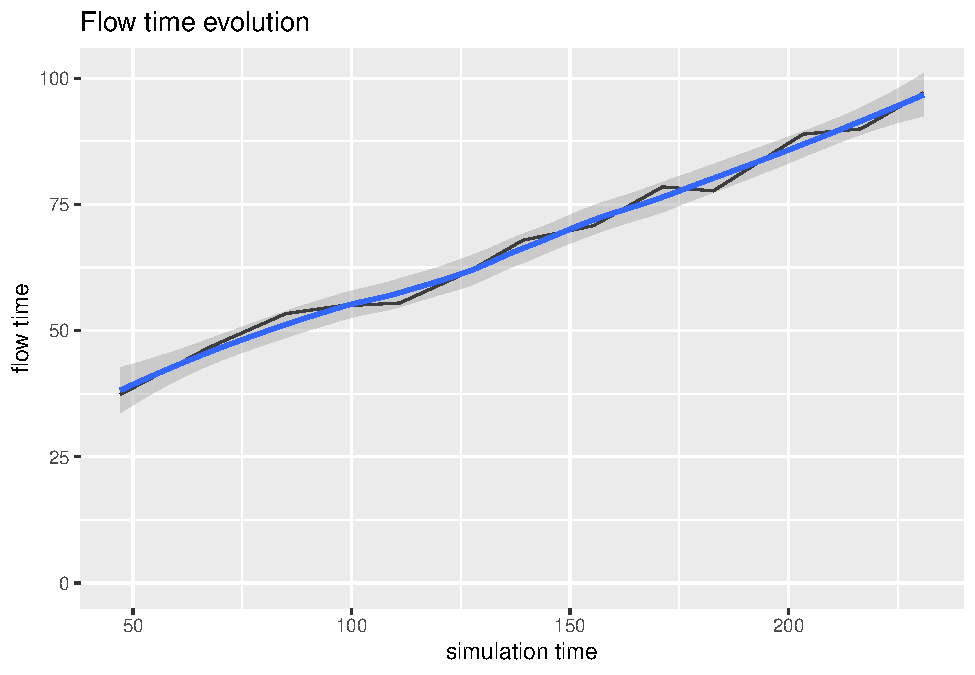
\includegraphics{SimBook_files/figure-latex/unnamed-chunk-6-1} 

}

\caption{Time spent in the health center}\label{fig:unnamed-chunk-6}
\end{figure}

Last Figure 1.6 reports the average time spent by patients in the health center. We can see that as the simulation clock increases, patients spend more time in the health center. From the previous plots, we can deduce that in general patients wait for the nurse, who has been busy all the time during the simulation.

\hypertarget{whats-next}{%
\section{What's next}\label{whats-next}}

The previous examples should have given you an idea of what a simulation model is and what you will be able to implement by the end of the course. However, it will take some time before we get to actually simulate systems. There are various skills that you will need to learn or revise before being able to implement simulation in R yourself. Specifically:

\begin{itemize}
\item
  first we will review the basics of R programming;
\item
  we will then review basic elements of probability and statistics;
\item
  we will discuss how randomness is implemented in programming languages and in R;
\item
  at this stage you will be able to implement your first simple simulations. In particular we will start with static simulation, also called \emph{Monte Carlo} simulation
\item
  we will then look at dynamic simulations as in the previous examples.
\end{itemize}

\hypertarget{r-programming}{%
\chapter{R programming}\label{r-programming}}

R is a programming language most commonly used within the statistical and machine learning community. This chapter will review some of the elements of R programming that will be used in later chapters. Do not expect this chapter to be exhaustive or self-contained. It is intended to give a quick refresh of R for users that have at least some experience with this programming language. There are many topics and concepts which are fundamental but will not be reviewed in this chapter. However, you should aim to master the topics included in this chapter since they will appear again later on in these notes. There are many other resources if you want to have a more in-depth look into R programming.

\begin{itemize}
\item
  The books of Hadley Wickham are surely a great starting point and are all available \href{http://hadley.nz/}{here}.
\item
  If you are unsure on how to do something with R, Google it!!! The community of R users is so wide that surely someone else has already asked your same question.
\item
  The R help is extremely useful and comprehensive. If you want to know more about a function, suppose it is called function, you can type \texttt{?function}.
\end{itemize}

\hypertarget{why-r}{%
\section{Why R?}\label{why-r}}

As mentioned in the previous chapter, simulation is very often applied in many areas, for instance management science and engineering. Often a simulation is carried out using an Excel spreadsheet or using a specialised software whose only purpose is creating simulations. Historically, R has not been at the forefront of the implementation of simulation models, in particular of discrete-event simulations. Only recently, R packages implementing discrete-event simulation have appeared, most importantly the \texttt{simmer} R package that you will learn using in later chapters.

These notes are intended to provide a unique view of simulation with specific implementation in the R programming language. Some of the strenght of R are:

\begin{itemize}
\item
  it is free, open-source and available in all major operating systems;
\item
  the community of R users is huge, with many forums, sites and resources that give you practical support in developing your own code;
\item
  a massive set of add-on packages to increase the capabilities of the basic R environment;
\item
  functions to perform state-of-the-art statistical and machine-learning methods. Researchers sometimes create an associated R package to any article they publish so for others to use their methods;
\item
  the integrated development environment RStudio provides a user-friendly environment to make the R programming experience more pleasing;
\item
  powerful communication tools to create documents and presentations embedding R code and R output. As a matter of fact this very book is created in R!!!!
\end{itemize}

\hypertarget{r-basics}{%
\section{R basics}\label{r-basics}}

So let's get started with R programming!

\hypertarget{r-as-a-calculator}{%
\subsection{R as a calculator}\label{r-as-a-calculator}}

In its most basic usage, we can use R as a calculator. Basic algebraic operations can be carried out as you would expect. The symbol \texttt{+} is for sum, \texttt{-} for subtraction, \texttt{*} for multiplication and \texttt{/} for division. Here are some examples:

\begin{Shaded}
\begin{Highlighting}[]
\DecValTok{4} \SpecialCharTok{+} \DecValTok{2}
\end{Highlighting}
\end{Shaded}

\begin{verbatim}
## [1] 6
\end{verbatim}

\begin{Shaded}
\begin{Highlighting}[]
\DecValTok{4} \SpecialCharTok{{-}} \DecValTok{2}
\end{Highlighting}
\end{Shaded}

\begin{verbatim}
## [1] 2
\end{verbatim}

\begin{Shaded}
\begin{Highlighting}[]
\DecValTok{4} \SpecialCharTok{*} \DecValTok{2}
\end{Highlighting}
\end{Shaded}

\begin{verbatim}
## [1] 8
\end{verbatim}

\begin{Shaded}
\begin{Highlighting}[]
\DecValTok{5} \SpecialCharTok{/} \DecValTok{2}
\end{Highlighting}
\end{Shaded}

\begin{verbatim}
## [1] 2.5
\end{verbatim}

\hypertarget{variable-assignment}{%
\subsection{Variable assignment}\label{variable-assignment}}

In R the symbol \texttt{\textless{}-} is used to assign a quantity to a variable. For instance, \texttt{a\ \textless{}-\ 4} assigns the number \texttt{4} to the variable \texttt{a} and \texttt{b\ \textless{}-\ 3} assigns the number \texttt{3} to \texttt{b}. It is much more common to work with variables in programming. Basic operations can then be performed over variables.

\begin{Shaded}
\begin{Highlighting}[]
\NormalTok{a }\OtherTok{\textless{}{-}} \DecValTok{4}
\NormalTok{b }\OtherTok{\textless{}{-}} \DecValTok{3}
\NormalTok{a }\SpecialCharTok{+}\NormalTok{ b}
\end{Highlighting}
\end{Shaded}

\begin{verbatim}
## [1] 7
\end{verbatim}

\begin{Shaded}
\begin{Highlighting}[]
\NormalTok{a }\SpecialCharTok{{-}}\NormalTok{ b}
\end{Highlighting}
\end{Shaded}

\begin{verbatim}
## [1] 1
\end{verbatim}

Notice for example that the code \texttt{a\ \textless{}-\ 4} does not show us the value of the variable \texttt{a}. It only creates this assignment. If we want to print the value of a variable, we have to explictly type the name of the variable.

\begin{Shaded}
\begin{Highlighting}[]
\NormalTok{a}
\end{Highlighting}
\end{Shaded}

\begin{verbatim}
## [1] 4
\end{verbatim}

\hypertarget{data-types}{%
\subsection{Data types}\label{data-types}}

In the previous examples we worked with numbers, but variables could be assigned other types of information. There are four basic types:

\begin{itemize}
\item
  \emph{Logicals} or \emph{Booleans}: corresponding to \texttt{TRUE} and \texttt{FALSE}, also abbreviated as \texttt{T} and \texttt{F} respectively;
\item
  \emph{Doubles}: real numbers;
\item
  \emph{Characters}: strings of text surrounded by \texttt{"} (for example \texttt{"hi"}) or by \texttt{\textquotesingle{}} (for example `by');
\item
  \emph{Integers}: integer numbers. If you type an integer in R, as before 3 or 4, it will usually be stored as a double unless explicitly defined.
\end{itemize}

Examples:

\begin{Shaded}
\begin{Highlighting}[]
\NormalTok{a }\OtherTok{\textless{}{-}} \ConstantTok{TRUE}
\NormalTok{a}
\end{Highlighting}
\end{Shaded}

\begin{verbatim}
## [1] TRUE
\end{verbatim}

\begin{Shaded}
\begin{Highlighting}[]
\NormalTok{b }\OtherTok{\textless{}{-}} \StringTok{"hello"}
\NormalTok{b}
\end{Highlighting}
\end{Shaded}

\begin{verbatim}
## [1] "hello"
\end{verbatim}

\hypertarget{vectors}{%
\subsection{Vectors}\label{vectors}}

In all previous examples the variables included one element only. More generally we can define sequences of elements or so-called \emph{vectors}. They can be defined with the command \texttt{c}, which stands for combine.

\begin{Shaded}
\begin{Highlighting}[]
\NormalTok{vec }\OtherTok{\textless{}{-}} \FunctionTok{c}\NormalTok{(}\DecValTok{1}\NormalTok{,}\DecValTok{3}\NormalTok{,}\DecValTok{5}\NormalTok{,}\DecValTok{7}\NormalTok{)}
\NormalTok{vec}
\end{Highlighting}
\end{Shaded}

\begin{verbatim}
## [1] 1 3 5 7
\end{verbatim}

So \texttt{vec} includes the sequence of numbers 1, 3, 5, 7. Notice that a vector can only include one data type. Consider the following:

\begin{Shaded}
\begin{Highlighting}[]
\NormalTok{vec }\OtherTok{\textless{}{-}} \FunctionTok{c}\NormalTok{(}\DecValTok{1}\NormalTok{, }\StringTok{"hello"}\NormalTok{, }\ConstantTok{TRUE}\NormalTok{)}
\NormalTok{vec}
\end{Highlighting}
\end{Shaded}

\begin{verbatim}
## [1] "1"     "hello" "TRUE"
\end{verbatim}

We created a variable \texttt{vec} where the first entry is a number, then a character string, then a Boolean. When we print \texttt{vec}, we get that its elements are \texttt{"1"}, \texttt{"hello"} and \texttt{"TRUE"}: it has transformed the number \texttt{1} into the string \texttt{"1"} and the Boolean \texttt{TRUE} into \texttt{"TRUE"}.

\hypertarget{matrices}{%
\subsection{Matrices}\label{matrices}}

Matrices are tables of elements that are organized in rows and columns. You can think of them as an arrangement of vectors into a table. Matrices must have the same data type in all its entries, as for vectors. Matrices can be constructed in multiple ways. One way is by stacking vectors into a matrix row-by-row with the command \texttt{rbind}. Consider the following example.

\begin{Shaded}
\begin{Highlighting}[]
\NormalTok{row1 }\OtherTok{\textless{}{-}} \FunctionTok{c}\NormalTok{(}\DecValTok{1}\NormalTok{,}\DecValTok{2}\NormalTok{,}\DecValTok{3}\NormalTok{)}
\NormalTok{row2 }\OtherTok{\textless{}{-}} \FunctionTok{c}\NormalTok{(}\DecValTok{4}\NormalTok{,}\DecValTok{5}\NormalTok{,}\DecValTok{6}\NormalTok{)}
\NormalTok{row3 }\OtherTok{\textless{}{-}} \FunctionTok{c}\NormalTok{(}\DecValTok{7}\NormalTok{,}\DecValTok{8}\NormalTok{,}\DecValTok{9}\NormalTok{)}
\NormalTok{mat }\OtherTok{\textless{}{-}} \FunctionTok{rbind}\NormalTok{(row1,row2,row3)}
\NormalTok{mat}
\end{Highlighting}
\end{Shaded}

\begin{verbatim}
##      [,1] [,2] [,3]
## row1    1    2    3
## row2    4    5    6
## row3    7    8    9
\end{verbatim}

So first we created vectors \texttt{row1\ =\ (1,2,3)}, \texttt{row2\ =\ (4,5,6)} and \texttt{row3\ =\ (7,8,9)} and then organizing them together into the matrix \texttt{mat}.

The following code follows the same procedure but now organizes vectors by columns instead using the command \texttt{cbind}.

\begin{Shaded}
\begin{Highlighting}[]
\NormalTok{col1 }\OtherTok{\textless{}{-}} \FunctionTok{c}\NormalTok{(}\DecValTok{1}\NormalTok{,}\DecValTok{2}\NormalTok{,}\DecValTok{3}\NormalTok{)}
\NormalTok{col2 }\OtherTok{\textless{}{-}} \FunctionTok{c}\NormalTok{(}\DecValTok{4}\NormalTok{,}\DecValTok{5}\NormalTok{,}\DecValTok{6}\NormalTok{)}
\NormalTok{col3 }\OtherTok{\textless{}{-}} \FunctionTok{c}\NormalTok{(}\DecValTok{7}\NormalTok{,}\DecValTok{8}\NormalTok{,}\DecValTok{9}\NormalTok{)}
\NormalTok{mat }\OtherTok{\textless{}{-}} \FunctionTok{cbind}\NormalTok{(col1,col2,col3)}
\NormalTok{mat}
\end{Highlighting}
\end{Shaded}

\begin{verbatim}
##      col1 col2 col3
## [1,]    1    4    7
## [2,]    2    5    8
## [3,]    3    6    9
\end{verbatim}

Last, there is also a command called \texttt{matrix} to create a matrix. It takes a vector, defined using the command \texttt{c} and stores its entries into a matrix of \texttt{nrow} rows and \texttt{ncol} columns. Consider the following example.

\begin{Shaded}
\begin{Highlighting}[]
\NormalTok{vec }\OtherTok{\textless{}{-}} \FunctionTok{c}\NormalTok{(}\DecValTok{1}\NormalTok{,}\DecValTok{2}\NormalTok{,}\DecValTok{3}\NormalTok{,}\DecValTok{4}\NormalTok{,}\DecValTok{5}\NormalTok{,}\DecValTok{6}\NormalTok{,}\DecValTok{7}\NormalTok{,}\DecValTok{8}\NormalTok{,}\DecValTok{9}\NormalTok{)}
\NormalTok{mat }\OtherTok{\textless{}{-}} \FunctionTok{matrix}\NormalTok{(vec, }\AttributeTok{nrow =} \DecValTok{3}\NormalTok{, }\AttributeTok{ncol =} \DecValTok{3}\NormalTok{)}
\NormalTok{mat}
\end{Highlighting}
\end{Shaded}

\begin{verbatim}
##      [,1] [,2] [,3]
## [1,]    1    4    7
## [2,]    2    5    8
## [3,]    3    6    9
\end{verbatim}

So first we created a vector \texttt{vec} with numbers from 1 to 9 and then stored them in a matrix with 3 rows and 3 columns. Number are stored by column: the first element of \texttt{vec} is in entry (1,1), the second element of \texttt{vec} is in entry (2,1), and so on.

\hypertarget{dataframes}{%
\subsection{Dataframes}\label{dataframes}}

Dataframes are very similar as matrices, they are tables organized in rows and columns. However, different to matrices they can have columns with different data types. They can be created with the command \texttt{data.frame}.

\begin{Shaded}
\begin{Highlighting}[]
\NormalTok{data }\OtherTok{\textless{}{-}} \FunctionTok{data.frame}\NormalTok{(}\AttributeTok{X1 =} \FunctionTok{c}\NormalTok{(}\DecValTok{1}\NormalTok{,}\DecValTok{2}\NormalTok{,}\DecValTok{3}\NormalTok{), }\AttributeTok{X2 =} \FunctionTok{c}\NormalTok{(}\ConstantTok{TRUE}\NormalTok{,}\ConstantTok{FALSE}\NormalTok{,}\ConstantTok{FALSE}\NormalTok{),}
                   \AttributeTok{X3 =} \FunctionTok{c}\NormalTok{(}\StringTok{"male"}\NormalTok{,}\StringTok{"male"}\NormalTok{,}\StringTok{"female"}\NormalTok{))}
\NormalTok{data}
\end{Highlighting}
\end{Shaded}

\begin{verbatim}
##   X1    X2     X3
## 1  1  TRUE   male
## 2  2 FALSE   male
## 3  3 FALSE female
\end{verbatim}

The dataframe \texttt{data} includes three columns: the first column \texttt{X1} of numbers, the second column \texttt{X2} of Boolean and the third column \texttt{X3} of characters. Dataframes are the objects that are most commonly used in real world data analysis.

\hypertarget{null-and-na}{%
\subsection{\texorpdfstring{\texttt{NULL} and \texttt{NA}}{NULL and NA}}\label{null-and-na}}

The expression \texttt{NA} is used in R to denote a missing value. Consider the following example.

\begin{Shaded}
\begin{Highlighting}[]
\NormalTok{vec }\OtherTok{\textless{}{-}} \FunctionTok{c}\NormalTok{(}\DecValTok{3}\NormalTok{, }\ConstantTok{NA}\NormalTok{, }\DecValTok{5}\NormalTok{)}
\NormalTok{vec}
\end{Highlighting}
\end{Shaded}

\begin{verbatim}
## [1]  3 NA  5
\end{verbatim}

Although the second element of \texttt{vec} is the expression \texttt{NA}, R recognizes that it is used for missing value and therefore the elements 3 and 5 are still considered numbers: indeed they are not printed as \texttt{"3"} and \texttt{"5"}.

\texttt{NULL} is an additional datatype. This can have various uses. For instance, it is associated to a vector with no entries.

\begin{Shaded}
\begin{Highlighting}[]
\FunctionTok{c}\NormalTok{()}
\end{Highlighting}
\end{Shaded}

\begin{verbatim}
## NULL
\end{verbatim}

\hypertarget{accessing-and-manipulating-variables}{%
\section{Accessing and manipulating variables}\label{accessing-and-manipulating-variables}}

Now that we have described the main objects we will work with in R, we can discuss how to access specific information.

\hypertarget{accessing-a-single-element}{%
\subsection{Accessing a single element}\label{accessing-a-single-element}}

Given a vector \texttt{vec} we can access its i-th entry with \texttt{vec{[}i{]}}.

\begin{Shaded}
\begin{Highlighting}[]
\NormalTok{vec }\OtherTok{\textless{}{-}} \FunctionTok{c}\NormalTok{(}\DecValTok{1}\NormalTok{,}\DecValTok{3}\NormalTok{,}\DecValTok{5}\NormalTok{)}
\NormalTok{vec[}\DecValTok{2}\NormalTok{]}
\end{Highlighting}
\end{Shaded}

\begin{verbatim}
## [1] 3
\end{verbatim}

For a matrix or a dataframe we need to specify the associated row and column. If we have a matrix \texttt{mat} we can access the element in entry (i,j) with \texttt{mat{[}i,j{]}}.

\begin{Shaded}
\begin{Highlighting}[]
\NormalTok{mat }\OtherTok{\textless{}{-}} \FunctionTok{matrix}\NormalTok{(}\FunctionTok{c}\NormalTok{(}\DecValTok{1}\NormalTok{,}\DecValTok{2}\NormalTok{,}\DecValTok{3}\NormalTok{,}\DecValTok{4}\NormalTok{,}\DecValTok{5}\NormalTok{,}\DecValTok{6}\NormalTok{,}\DecValTok{7}\NormalTok{,}\DecValTok{8}\NormalTok{,}\DecValTok{9}\NormalTok{), }\AttributeTok{ncol=}\DecValTok{3}\NormalTok{, }\AttributeTok{nrow =}\DecValTok{3}\NormalTok{)}
\NormalTok{mat[}\DecValTok{1}\NormalTok{,}\DecValTok{3}\NormalTok{]}
\end{Highlighting}
\end{Shaded}

\begin{verbatim}
## [1] 7
\end{verbatim}

\hypertarget{acessing-multiple-entries}{%
\subsection{Acessing multiple entries}\label{acessing-multiple-entries}}

To access multiple entries we can on the other hand define a vector of indexes of the elements we want to access. Consider the following examples:

\begin{Shaded}
\begin{Highlighting}[]
\NormalTok{vec }\OtherTok{\textless{}{-}} \FunctionTok{c}\NormalTok{(}\DecValTok{1}\NormalTok{,}\DecValTok{3}\NormalTok{,}\DecValTok{5}\NormalTok{)}
\NormalTok{vec[}\FunctionTok{c}\NormalTok{(}\DecValTok{1}\NormalTok{,}\DecValTok{2}\NormalTok{)]}
\end{Highlighting}
\end{Shaded}

\begin{verbatim}
## [1] 1 3
\end{verbatim}

The above code accesses the first two entries of the vector \texttt{vec}. To do this we had to define a vector using \texttt{c(1,2)} stating the entries we wanted to look at. For matrices consider:

\begin{Shaded}
\begin{Highlighting}[]
\NormalTok{mat }\OtherTok{\textless{}{-}} \FunctionTok{matrix}\NormalTok{(}\FunctionTok{c}\NormalTok{(}\DecValTok{1}\NormalTok{,}\DecValTok{2}\NormalTok{,}\DecValTok{3}\NormalTok{,}\DecValTok{4}\NormalTok{,}\DecValTok{5}\NormalTok{,}\DecValTok{6}\NormalTok{,}\DecValTok{7}\NormalTok{,}\DecValTok{8}\NormalTok{,}\DecValTok{9}\NormalTok{), }\AttributeTok{ncol=}\DecValTok{3}\NormalTok{, }\AttributeTok{nrow =}\DecValTok{3}\NormalTok{)}
\NormalTok{mat[}\FunctionTok{c}\NormalTok{(}\DecValTok{1}\NormalTok{,}\DecValTok{2}\NormalTok{),}\FunctionTok{c}\NormalTok{(}\DecValTok{2}\NormalTok{,}\DecValTok{3}\NormalTok{)]}
\end{Highlighting}
\end{Shaded}

\begin{verbatim}
##      [,1] [,2]
## [1,]    4    7
## [2,]    5    8
\end{verbatim}

The syntax is very similar as before. We defined to index vectors, one for the rows and one for columns. The two statements \texttt{c(1,2)} and \texttt{c(2,3)} are separated by a comma to denote that the first selects the first and second row, whilst the second selects the second and third column.

If one wants to access full rows or full columns, the argument associated to rows or columns is left blank. Consider the following examples.

\begin{Shaded}
\begin{Highlighting}[]
\NormalTok{mat }\OtherTok{\textless{}{-}} \FunctionTok{matrix}\NormalTok{(}\FunctionTok{c}\NormalTok{(}\DecValTok{1}\NormalTok{,}\DecValTok{2}\NormalTok{,}\DecValTok{3}\NormalTok{,}\DecValTok{4}\NormalTok{,}\DecValTok{5}\NormalTok{,}\DecValTok{6}\NormalTok{,}\DecValTok{7}\NormalTok{,}\DecValTok{8}\NormalTok{,}\DecValTok{9}\NormalTok{), }\AttributeTok{ncol=}\DecValTok{3}\NormalTok{, }\AttributeTok{nrow =}\DecValTok{3}\NormalTok{)}
\NormalTok{mat[}\DecValTok{1}\NormalTok{,]}
\end{Highlighting}
\end{Shaded}

\begin{verbatim}
## [1] 1 4 7
\end{verbatim}

\begin{Shaded}
\begin{Highlighting}[]
\NormalTok{mat[,}\FunctionTok{c}\NormalTok{(}\DecValTok{1}\NormalTok{,}\DecValTok{2}\NormalTok{)]}
\end{Highlighting}
\end{Shaded}

\begin{verbatim}
##      [,1] [,2]
## [1,]    1    4
## [2,]    2    5
## [3,]    3    6
\end{verbatim}

The code \texttt{mat{[}1,{]}} selects the first full row of \texttt{mat}. The code \texttt{mat{[},c(1,2){]}} selects the first and second column of \texttt{mat}. Notice that the comma has always to be included!

To access multiple entries it is often useful to define sequences of number quickly. The following command defines the sequence of integer numbers from 1 to 9.

\begin{Shaded}
\begin{Highlighting}[]
\DecValTok{1}\SpecialCharTok{:}\DecValTok{9}
\end{Highlighting}
\end{Shaded}

\begin{verbatim}
## [1] 1 2 3 4 5 6 7 8 9
\end{verbatim}

More generally, one can define sequences of numbers using \texttt{seq} (see \texttt{?seq}).

\hypertarget{accessing-entries-with-logical-operators}{%
\subsection{Accessing entries with logical operators}\label{accessing-entries-with-logical-operators}}

If we want to access elements of an object based on a condition it is often easier to use logical operators. This means comparing entries using the comparisons you would usually use in mathematical reasoning, for instance being equal to, or being larger to. The syntax is as follows:

\begin{itemize}
\item
  \texttt{==} to check equality (notice the two equal signs)
\item
  \texttt{!=} to check non-equality
\item
  \texttt{\textgreater{}} bigger to
\item
  \texttt{\textgreater{}=} bigger or equal to
\item
  \texttt{\textless{}} less to
\item
  \texttt{\textless{}=} less or equal to
\end{itemize}

Let's see some examples.

\begin{Shaded}
\begin{Highlighting}[]
\NormalTok{vec }\OtherTok{\textless{}{-}} \FunctionTok{c}\NormalTok{(}\DecValTok{2}\NormalTok{,}\DecValTok{3}\NormalTok{,}\DecValTok{4}\NormalTok{,}\DecValTok{5}\NormalTok{,}\DecValTok{6}\NormalTok{)}
\NormalTok{vec }\SpecialCharTok{\textgreater{}} \DecValTok{4}
\end{Highlighting}
\end{Shaded}

\begin{verbatim}
## [1] FALSE FALSE FALSE  TRUE  TRUE
\end{verbatim}

We constructed a vector \texttt{vec} and check which entries were larger than 4. The output is a Boolean vector with the same number of entries as \texttt{vec} where only the last two entries are \texttt{TRUE}. Similarly,

\begin{Shaded}
\begin{Highlighting}[]
\NormalTok{vec }\OtherTok{\textless{}{-}} \FunctionTok{c}\NormalTok{(}\DecValTok{2}\NormalTok{,}\DecValTok{3}\NormalTok{,}\DecValTok{4}\NormalTok{,}\DecValTok{5}\NormalTok{,}\DecValTok{6}\NormalTok{)}
\NormalTok{vec }\SpecialCharTok{==} \DecValTok{4}
\end{Highlighting}
\end{Shaded}

\begin{verbatim}
## [1] FALSE FALSE  TRUE FALSE FALSE
\end{verbatim}

has a \texttt{TRUE} in the third entry only.

So if we were to be interested in returning the elements of \texttt{vec} that are larger than 4 we could use the code

\begin{Shaded}
\begin{Highlighting}[]
\NormalTok{vec }\OtherTok{\textless{}{-}} \FunctionTok{c}\NormalTok{(}\DecValTok{2}\NormalTok{,}\DecValTok{3}\NormalTok{,}\DecValTok{4}\NormalTok{,}\DecValTok{5}\NormalTok{,}\DecValTok{6}\NormalTok{)}
\NormalTok{vec[vec }\SpecialCharTok{\textgreater{}} \DecValTok{4}\NormalTok{]}
\end{Highlighting}
\end{Shaded}

\begin{verbatim}
## [1] 5 6
\end{verbatim}

So we have a vector with only elements 5 and 6.

\hypertarget{manipulating-dataframes}{%
\subsection{Manipulating dataframes}\label{manipulating-dataframes}}

We have seen in the previous section that dataframes are special types of matrices where columns can include a different data type. For this reason they have special way to manipulate and access their entries.

First, specific columns of a dataframe can be accessed using its name and the \texttt{\$} sign as follows.

\begin{Shaded}
\begin{Highlighting}[]
\NormalTok{data }\OtherTok{\textless{}{-}} \FunctionTok{data.frame}\NormalTok{(}\AttributeTok{X1 =} \FunctionTok{c}\NormalTok{(}\DecValTok{1}\NormalTok{,}\DecValTok{2}\NormalTok{,}\DecValTok{3}\NormalTok{), }\AttributeTok{X2 =} \FunctionTok{c}\NormalTok{(}\ConstantTok{TRUE}\NormalTok{,}\ConstantTok{FALSE}\NormalTok{,}\ConstantTok{FALSE}\NormalTok{),}
                   \AttributeTok{X3 =} \FunctionTok{c}\NormalTok{(}\StringTok{"male"}\NormalTok{,}\StringTok{"male"}\NormalTok{,}\StringTok{"female"}\NormalTok{))}
\NormalTok{data}\SpecialCharTok{$}\NormalTok{X1}
\end{Highlighting}
\end{Shaded}

\begin{verbatim}
## [1] 1 2 3
\end{verbatim}

\begin{Shaded}
\begin{Highlighting}[]
\NormalTok{data}\SpecialCharTok{$}\NormalTok{X3}
\end{Highlighting}
\end{Shaded}

\begin{verbatim}
## [1] male   male   female
## Levels: female male
\end{verbatim}

So using the name of the dataframe \texttt{data} followed by \texttt{\$} and then the name of the column, for instance \texttt{X1}, we access that specific column of the dataframe.

Second, we can use the \texttt{\$} sign to add new columns to a dataframe. Consider the following code.

\begin{Shaded}
\begin{Highlighting}[]
\NormalTok{data }\OtherTok{\textless{}{-}} \FunctionTok{data.frame}\NormalTok{(}\AttributeTok{X1 =} \FunctionTok{c}\NormalTok{(}\DecValTok{1}\NormalTok{,}\DecValTok{2}\NormalTok{,}\DecValTok{3}\NormalTok{), }\AttributeTok{X2 =} \FunctionTok{c}\NormalTok{(}\ConstantTok{TRUE}\NormalTok{,}\ConstantTok{FALSE}\NormalTok{,}\ConstantTok{FALSE}\NormalTok{),}
                   \AttributeTok{X3 =} \FunctionTok{c}\NormalTok{(}\StringTok{"male"}\NormalTok{,}\StringTok{"male"}\NormalTok{,}\StringTok{"female"}\NormalTok{))}
\NormalTok{data}\SpecialCharTok{$}\NormalTok{X4 }\OtherTok{\textless{}{-}} \FunctionTok{c}\NormalTok{(}\StringTok{"yes"}\NormalTok{,}\StringTok{"no"}\NormalTok{,}\StringTok{"no"}\NormalTok{)}
\NormalTok{data}
\end{Highlighting}
\end{Shaded}

\begin{verbatim}
##   X1    X2     X3  X4
## 1  1  TRUE   male yes
## 2  2 FALSE   male  no
## 3  3 FALSE female  no
\end{verbatim}

\texttt{data} now includes a fourth column called \texttt{X4} coinciding to the vector \texttt{c("yes","no","no")}.

Third, we can select specific rows of a dataframe using the command \texttt{subset}. Consider the following example.

\begin{Shaded}
\begin{Highlighting}[]
\NormalTok{data }\OtherTok{\textless{}{-}} \FunctionTok{data.frame}\NormalTok{(}\AttributeTok{X1 =} \FunctionTok{c}\NormalTok{(}\DecValTok{1}\NormalTok{,}\DecValTok{2}\NormalTok{,}\DecValTok{3}\NormalTok{), }\AttributeTok{X2 =} \FunctionTok{c}\NormalTok{(}\ConstantTok{TRUE}\NormalTok{,}\ConstantTok{FALSE}\NormalTok{,}\ConstantTok{FALSE}\NormalTok{),}
                   \AttributeTok{X3 =} \FunctionTok{c}\NormalTok{(}\StringTok{"male"}\NormalTok{,}\StringTok{"male"}\NormalTok{,}\StringTok{"female"}\NormalTok{))}
\FunctionTok{subset}\NormalTok{(data, X1 }\SpecialCharTok{\textless{}=} \DecValTok{2}\NormalTok{)}
\end{Highlighting}
\end{Shaded}

\begin{verbatim}
##   X1    X2   X3
## 1  1  TRUE male
## 2  2 FALSE male
\end{verbatim}

The above code returns the rows of \texttt{data} such that \texttt{X1} is less or equal to 2. More complex rules to subset a dataframe can be combined using the and operator \texttt{\&} and the or operator \texttt{\textbar{}}. Let's see an example.

\begin{Shaded}
\begin{Highlighting}[]
\NormalTok{data }\OtherTok{\textless{}{-}} \FunctionTok{data.frame}\NormalTok{(}\AttributeTok{X1 =} \FunctionTok{c}\NormalTok{(}\DecValTok{1}\NormalTok{,}\DecValTok{2}\NormalTok{,}\DecValTok{3}\NormalTok{), }\AttributeTok{X2 =} \FunctionTok{c}\NormalTok{(}\ConstantTok{TRUE}\NormalTok{,}\ConstantTok{FALSE}\NormalTok{,}\ConstantTok{FALSE}\NormalTok{),}
                   \AttributeTok{X3 =} \FunctionTok{c}\NormalTok{(}\StringTok{"male"}\NormalTok{,}\StringTok{"male"}\NormalTok{,}\StringTok{"female"}\NormalTok{))}
\FunctionTok{subset}\NormalTok{(data, X1 }\SpecialCharTok{\textless{}=} \DecValTok{2} \SpecialCharTok{\&}\NormalTok{ X2 }\SpecialCharTok{==} \ConstantTok{TRUE}\NormalTok{)}
\end{Highlighting}
\end{Shaded}

\begin{verbatim}
##   X1   X2   X3
## 1  1 TRUE male
\end{verbatim}

So the above code selects the rows such that \texttt{X1} is less or equal to 2 and \texttt{X2} is \texttt{TRUE}. This is the case only for the first row of \texttt{data}.

\hypertarget{information-about-objects}{%
\subsection{Information about objects}\label{information-about-objects}}

Here is a list of functions which are often useful to get information about objects in R.

\begin{itemize}
\item
  \texttt{length} returns the number of entries in a vector.
\item
  \texttt{dim} returns the number of rows and columns of a matrix or a dataframe
\item
  \texttt{unique} returns the unique elements of a vector or the unique rows of a matrix or a dataframe.
\item
  \texttt{head} returns the first entries of a vector or the first rows of a matrix or a dataframe
\item
  \texttt{order} returns a re-ordering of a vector or a data.frame in ascending order.
\end{itemize}

Let's see some examples.

\begin{Shaded}
\begin{Highlighting}[]
\NormalTok{vec }\OtherTok{\textless{}{-}} \FunctionTok{c}\NormalTok{(}\DecValTok{4}\NormalTok{,}\DecValTok{2}\NormalTok{,}\DecValTok{7}\NormalTok{,}\DecValTok{5}\NormalTok{,}\DecValTok{5}\NormalTok{)}
\FunctionTok{length}\NormalTok{(vec)}
\end{Highlighting}
\end{Shaded}

\begin{verbatim}
## [1] 5
\end{verbatim}

\begin{Shaded}
\begin{Highlighting}[]
\FunctionTok{unique}\NormalTok{(vec)}
\end{Highlighting}
\end{Shaded}

\begin{verbatim}
## [1] 4 2 7 5
\end{verbatim}

\begin{Shaded}
\begin{Highlighting}[]
\FunctionTok{order}\NormalTok{(vec)}
\end{Highlighting}
\end{Shaded}

\begin{verbatim}
## [1] 2 1 4 5 3
\end{verbatim}

\texttt{length} gives the number of elements of \texttt{vec}, \texttt{unique} returns the different values in \texttt{vec} (so 5 is not repeated), \texttt{order} returns in entry i the ordering of the i-th entry of \texttt{vec}. So the first entry of \texttt{order(vec)} is 2 since 4 is the second-smallest entry of \texttt{vec}.

\begin{Shaded}
\begin{Highlighting}[]
\NormalTok{data }\OtherTok{\textless{}{-}} \FunctionTok{data.frame}\NormalTok{(}\AttributeTok{X1 =} \FunctionTok{c}\NormalTok{(}\DecValTok{1}\NormalTok{,}\DecValTok{2}\NormalTok{,}\DecValTok{3}\NormalTok{,}\DecValTok{4}\NormalTok{), }\AttributeTok{X2 =} \FunctionTok{c}\NormalTok{(}\ConstantTok{TRUE}\NormalTok{,}\ConstantTok{FALSE}\NormalTok{,}\ConstantTok{FALSE}\NormalTok{,}\ConstantTok{FALSE}\NormalTok{),}
                   \AttributeTok{X3 =} \FunctionTok{c}\NormalTok{(}\StringTok{"male"}\NormalTok{,}\StringTok{"male"}\NormalTok{,}\StringTok{"female"}\NormalTok{,}\StringTok{"female"}\NormalTok{))}
\FunctionTok{dim}\NormalTok{(data)}
\end{Highlighting}
\end{Shaded}

\begin{verbatim}
## [1] 4 3
\end{verbatim}

So \texttt{dim} tells us that \texttt{data} has four rows and three columns.

\hypertarget{loops-and-conditions}{%
\section{Loops and conditions}\label{loops-and-conditions}}

This section reviews two of the most basic elements of any programming language: \texttt{if} statements and \texttt{cycles} or \texttt{loops}.

\hypertarget{if-statements}{%
\subsection{\texorpdfstring{\texttt{if} statements}{if statements}}\label{if-statements}}

The basic form of an \texttt{if} statement in R is as follows:

\begin{Shaded}
\begin{Highlighting}[]
\ControlFlowTok{if}\NormalTok{(condition)\{true\_action\}}
\end{Highlighting}
\end{Shaded}

Condition must return a Boolean, either \texttt{TRUE} or \texttt{FALSE}. If \texttt{TRUE} then the code follows the code within the curly brackets and performs the \texttt{true\_action}. If \texttt{condition} is \texttt{FALSE} the code does nothing.

It is more customary to also give a chunk of code for the case \texttt{condition} is \texttt{FALSE}. This can be achieved with \texttt{else}.

\begin{Shaded}
\begin{Highlighting}[]
\ControlFlowTok{if}\NormalTok{(condition)\{true\_action\} }\ControlFlowTok{else}\NormalTok{ \{false\_action\}}
\end{Highlighting}
\end{Shaded}

Let's see an example.

\begin{Shaded}
\begin{Highlighting}[]
\NormalTok{a }\OtherTok{\textless{}{-}} \DecValTok{5}
\ControlFlowTok{if}\NormalTok{ (a }\SpecialCharTok{\textless{}} \DecValTok{2}\NormalTok{)\{}\StringTok{"hello"}\NormalTok{\} }\ControlFlowTok{else}\NormalTok{ \{}\StringTok{"goodbye"}\NormalTok{\}}
\end{Highlighting}
\end{Shaded}

\begin{verbatim}
## [1] "goodbye"
\end{verbatim}

The variable \texttt{a} is assigned the number 5. Then we impose a condition: if \texttt{a} is less than 2, we print the text \texttt{"hello"}, otherwise \texttt{"goodbye"} is printed. Since \texttt{a\ \textless{}-\ 5} the code prints correctly \texttt{"goodbye"}. On the other hand if \texttt{a} were assigned \texttt{1}.

\begin{Shaded}
\begin{Highlighting}[]
\NormalTok{a }\OtherTok{\textless{}{-}} \DecValTok{1}
\ControlFlowTok{if}\NormalTok{ (a }\SpecialCharTok{\textless{}} \DecValTok{2}\NormalTok{)\{}\StringTok{"hello"}\NormalTok{\} }\ControlFlowTok{else}\NormalTok{ \{}\StringTok{"goodbye"}\NormalTok{\}}
\end{Highlighting}
\end{Shaded}

\begin{verbatim}
## [1] "hello"
\end{verbatim}

\hypertarget{ifelse}{%
\subsection{\texorpdfstring{\texttt{ifelse}}{ifelse}}\label{ifelse}}

\texttt{if} works when checking a single element and the condition returns either \texttt{TRUE} or \texttt{FALSE}. The command \texttt{ifelse} can be used to quickly check a condition over all elements of a vector. Consider the following example.

\begin{Shaded}
\begin{Highlighting}[]
\NormalTok{vec }\OtherTok{\textless{}{-}} \FunctionTok{c}\NormalTok{(}\DecValTok{1}\NormalTok{, }\DecValTok{3}\NormalTok{, }\DecValTok{5}\NormalTok{, }\DecValTok{7}\NormalTok{, }\DecValTok{9}\NormalTok{)}
\FunctionTok{ifelse}\NormalTok{(vec }\SpecialCharTok{\textgreater{}} \DecValTok{5}\NormalTok{, }\StringTok{"bigger"}\NormalTok{, }\StringTok{"smaller"}\NormalTok{)}
\end{Highlighting}
\end{Shaded}

\begin{verbatim}
## [1] "smaller" "smaller" "smaller" "bigger"  "bigger"
\end{verbatim}

\texttt{vec} contains the values 1, 3, 5, 7, 9 and the \texttt{condition} is if an elemenent of \texttt{vec} is larger than 5. If \texttt{TRUE} the code returns the string \texttt{bigger} and otherwise returns \texttt{smaller}. The code above returns therefore a vector of the same length of \texttt{vec} including either the string \texttt{bigger} or the string \texttt{smaller}.

\hypertarget{loops}{%
\subsection{Loops}\label{loops}}

\texttt{for} loops are used to iterate over items in a vector. They have the following skeleton:

\begin{Shaded}
\begin{Highlighting}[]
\ControlFlowTok{for}\NormalTok{(item }\ControlFlowTok{in}\NormalTok{ vector) \{perform\_action\}}
\end{Highlighting}
\end{Shaded}

For each \texttt{item} in \texttt{vector}, \texttt{perform\_action} is performed once and the value of \texttt{item} is updated each time.

Here is an example.

\begin{Shaded}
\begin{Highlighting}[]
\ControlFlowTok{for}\NormalTok{ (i }\ControlFlowTok{in} \FunctionTok{c}\NormalTok{(}\DecValTok{1}\NormalTok{,}\DecValTok{2}\NormalTok{,}\DecValTok{3}\NormalTok{))\{}
  \FunctionTok{print}\NormalTok{(i)}
\NormalTok{\}}
\end{Highlighting}
\end{Shaded}

\begin{verbatim}
## [1] 1
## [1] 2
## [1] 3
\end{verbatim}

Item is the variable \texttt{i} (it is costumary to use just a letter) and at each step \texttt{i} is set equal to a value in the vector \texttt{c(1,2,3)}. At each of these iterations, the command \texttt{print(i)}, which simply returns the value that \texttt{i} takes is called. Indeed we see that the output is the sequence of numbers 1, 2, 3.

\hypertarget{functions}{%
\section{Functions}\label{functions}}

Functions are chunks of code that are given a name so that they can be easily used multiple times. Perhaps without realising it, you have used functions already many times!

\hypertarget{defining-your-own-function}{%
\subsection{Defining your own function}\label{defining-your-own-function}}

A function is composed of the following elements:

\begin{itemize}
\item
  a name: in R functions are objects just like vectors or matrices and they are given a name.
\item
  arguments: these are objects that will be used within the function.
\item
  body: a chunk of code which is run within the function.
\item
  output: an object that the function returns.
\end{itemize}

Let's consider an example.

\begin{Shaded}
\begin{Highlighting}[]
\NormalTok{my.function }\OtherTok{\textless{}{-}} \ControlFlowTok{function}\NormalTok{(x,y)\{}
\NormalTok{  z }\OtherTok{\textless{}{-}}\NormalTok{ x }\SpecialCharTok{+}\NormalTok{ y}
  \FunctionTok{return}\NormalTok{(z)}
\NormalTok{\}}
\end{Highlighting}
\end{Shaded}

The above function computes the sum of two numbers \texttt{x} and \texttt{y}. Let's call it.

\begin{Shaded}
\begin{Highlighting}[]
\FunctionTok{my.function}\NormalTok{(}\DecValTok{2}\NormalTok{,}\DecValTok{3}\NormalTok{)}
\end{Highlighting}
\end{Shaded}

\begin{verbatim}
## [1] 5
\end{verbatim}

The sum between 2 and 3 is indeed 5.

Let's look at the code line by line. In the first line, we assigned a function using the command \texttt{function} to an object called \texttt{my.function}. \texttt{my.function} has two arguments called \texttt{x} and \texttt{y}. Then there is an opening curly bracket \texttt{\{}. The last line of code has a closing curly bracket \texttt{\}}: whatever is in between the two brackets is a chunk of code which is run when the function is run. The second line computes a new variable called \texttt{z} which stores the sum of \texttt{x} and \texttt{y}. The third line of code tells us that the function should return \texttt{z} as output.

Let's consider a slightly more complicated function.

\begin{Shaded}
\begin{Highlighting}[]
\NormalTok{new.function }\OtherTok{\textless{}{-}} \ControlFlowTok{function}\NormalTok{(x,y)\{}
\NormalTok{  z1 }\OtherTok{\textless{}{-}}\NormalTok{ x}\SpecialCharTok{\^{}}\DecValTok{2}
\NormalTok{  z2 }\OtherTok{\textless{}{-}}\NormalTok{ z1 }\SpecialCharTok{+}\NormalTok{ y}
  \FunctionTok{return}\NormalTok{(z2)}
\NormalTok{\}}
\end{Highlighting}
\end{Shaded}

The \texttt{new.function} returns the sum between the square of the first input \texttt{x} and the second input \texttt{y}. Let's call the function.

\begin{Shaded}
\begin{Highlighting}[]
\FunctionTok{new.function}\NormalTok{(}\DecValTok{2}\NormalTok{,}\DecValTok{3}\NormalTok{)}
\end{Highlighting}
\end{Shaded}

\begin{verbatim}
## [1] 7
\end{verbatim}

\begin{Shaded}
\begin{Highlighting}[]
\FunctionTok{new.function}\NormalTok{(}\DecValTok{3}\NormalTok{,}\DecValTok{2}\NormalTok{)}
\end{Highlighting}
\end{Shaded}

\begin{verbatim}
## [1] 11
\end{verbatim}

Notice that \texttt{new.function(2,3)} is different from \texttt{new.function(3,2)}: indeed in the fist case the sum between 2\^{}2 and 3 is computed, whilst in the second the sum between 3\^{}2 and 2 is computed. Furthermore, that the variable \texttt{z1} exists only within the function: when you call the function the output does not create a variable \texttt{z1}. The output does not create either a variable \texttt{z2} it simply returns the value that is stored in \texttt{z2}, which can the be assigned as in the following example.

\begin{Shaded}
\begin{Highlighting}[]
\NormalTok{value }\OtherTok{\textless{}{-}} \FunctionTok{new.function}\NormalTok{(}\DecValTok{2}\NormalTok{,}\DecValTok{3}\NormalTok{)}
\NormalTok{value}
\end{Highlighting}
\end{Shaded}

\begin{verbatim}
## [1] 7
\end{verbatim}

We stored in \texttt{value} the output of \texttt{new.function(2,3)}.

An equivalent way to write \texttt{new.function} is as follows:

\begin{Shaded}
\begin{Highlighting}[]
\NormalTok{new.function }\OtherTok{\textless{}{-}} \ControlFlowTok{function}\NormalTok{(x,y)\{}
\NormalTok{  x}\SpecialCharTok{\^{}}\DecValTok{2} \SpecialCharTok{+}\NormalTok{ y}
\NormalTok{\}}
\FunctionTok{new.function}\NormalTok{(}\DecValTok{2}\NormalTok{,}\DecValTok{3}\NormalTok{)}
\end{Highlighting}
\end{Shaded}

\begin{verbatim}
## [1] 7
\end{verbatim}

The output is the same. We did not create any variable within the function and we did not explicitly use the \texttt{return} command. R understands that the last line of code is what the function should return.

\hypertarget{calling-functions}{%
\subsection{Calling functions}\label{calling-functions}}

In R functions can be called in various ways. Before we have seen function calls as

\begin{Shaded}
\begin{Highlighting}[]
\FunctionTok{new.function}\NormalTok{(}\DecValTok{2}\NormalTok{,}\DecValTok{3}\NormalTok{)}
\end{Highlighting}
\end{Shaded}

How did it work?

\begin{itemize}
\item
  The function \texttt{new.function} has a first argument \texttt{x} and a second argument \texttt{y}.
\item
  R matched the first argument in \texttt{new.function(2,3)} to \texttt{x}, that is \texttt{x=2}, and the second argument to \texttt{y}, that is \texttt{y=3}.
\end{itemize}

We could have also been more explicit and state what \texttt{x} and \texttt{y} were.

\begin{Shaded}
\begin{Highlighting}[]
\FunctionTok{new.function}\NormalTok{(}\AttributeTok{x=}\DecValTok{2}\NormalTok{, }\AttributeTok{y=}\DecValTok{3}\NormalTok{)}
\end{Highlighting}
\end{Shaded}

\begin{verbatim}
## [1] 7
\end{verbatim}

So now explicitly we state that the input \texttt{x} of \texttt{new.function} is 2 and that the input \texttt{y} is 3. Notice that the two ways of specifying inputs give the exact same results.

\hypertarget{mathematical-and-statistical-functions}{%
\subsection{Mathematical and statistical functions}\label{mathematical-and-statistical-functions}}

The number of functions available in R is massive and it would be impossible to mention them all. Here I just give you a list of mathematical and statistical functions that we may use in the following.

\begin{itemize}
\item
  \texttt{exp} computes the exponential of the entries of an object
\item
  \texttt{log} computes the logarithm of the entries of an object
\item
  \texttt{sqrt} computes the square root of the entries of an
\item
  \texttt{sum} computes the sum of the entries of an object
\item
  \texttt{abs} computes the absolute value of the entries of an object
\item
  \texttt{mean} computes the mean of the entries of an object
\item
  \texttt{sd} computes the standard deviation of the entries of an object
\item
  \texttt{var} computes the variance of the entries of an object
\end{itemize}

\hypertarget{the-apply-family-of-functions}{%
\section{\texorpdfstring{The \texttt{apply} family of functions}{The apply family of functions}}\label{the-apply-family-of-functions}}

One of the biggest limitation of R is that it is slow in performing cycles. For this reason, one should aim at avoiding as much as possible to use of loops.

There are various functions which are designed to help you in avoiding these loops and they are in the family of so called \texttt{apply} functions. There are many of these but we will only see two here.

\hypertarget{the-function-apply}{%
\subsection{\texorpdfstring{The function \texttt{apply}}{The function apply}}\label{the-function-apply}}

Consider the following code.

\begin{Shaded}
\begin{Highlighting}[]
\NormalTok{x }\OtherTok{\textless{}{-}} \FunctionTok{matrix}\NormalTok{(}\FunctionTok{c}\NormalTok{(}\DecValTok{1}\SpecialCharTok{:}\DecValTok{9}\NormalTok{), }\AttributeTok{ncol=}\DecValTok{3}\NormalTok{ , }\AttributeTok{nrow =} \DecValTok{3}\NormalTok{)}
\NormalTok{y }\OtherTok{\textless{}{-}} \FunctionTok{c}\NormalTok{()}
\ControlFlowTok{for}\NormalTok{ (i }\ControlFlowTok{in} \DecValTok{1}\SpecialCharTok{:}\DecValTok{3}\NormalTok{)\{}
\NormalTok{  y[i] }\OtherTok{\textless{}{-}} \FunctionTok{sum}\NormalTok{(x[i,])}
\NormalTok{\}}
\NormalTok{y}
\end{Highlighting}
\end{Shaded}

\begin{verbatim}
## [1] 12 15 18
\end{verbatim}

The code first defines a matrix \texttt{x} and an empty vector \texttt{y} (recall that this is bad practice, but for this example it does not matter). Then there is a \texttt{for} cycle which assigns to the i-th entry of \texttt{y} the sum of the entries of the i-th row of \texttt{x}. So the vector \texttt{y} includes the row-totals.

For this simple example the \texttt{for} cycle is extremely quick, but this is just to illustrate how we can replace it using the \texttt{apply} function.

\begin{Shaded}
\begin{Highlighting}[]
\FunctionTok{apply}\NormalTok{(x, }\DecValTok{1}\NormalTok{, sum)}
\end{Highlighting}
\end{Shaded}

\begin{verbatim}
## [1] 12 15 18
\end{verbatim}

Let's look at the above code. The first input of \texttt{apply} is the object we want to operate upon, in this case the matrix \texttt{x}. The second input specifies if the operation has to act over the rows of the matrix (input equal to 1) or over the columns (input equal to 2). The third input is the operation we want to use, in this case \texttt{sum}.

Beside being faster, the above code is also a lot more compact than using a for loop.

The following example computes the mean of each column of \texttt{x}.

\begin{Shaded}
\begin{Highlighting}[]
\FunctionTok{apply}\NormalTok{(x, }\DecValTok{2}\NormalTok{, mean)}
\end{Highlighting}
\end{Shaded}

\begin{verbatim}
## [1] 2 5 8
\end{verbatim}

\hypertarget{the-function-sapply}{%
\subsection{\texorpdfstring{The function \texttt{sapply}}{The function sapply}}\label{the-function-sapply}}

Consider again our function \texttt{new.function} which computes the sum of the squared of a number \texttt{x} with another number \texttt{y}.

\begin{Shaded}
\begin{Highlighting}[]
\NormalTok{new.function }\OtherTok{\textless{}{-}} \ControlFlowTok{function}\NormalTok{(x,y)\{ x}\SpecialCharTok{\^{}}\DecValTok{2} \SpecialCharTok{+}\NormalTok{ y\}}
\end{Highlighting}
\end{Shaded}

Suppose that we want to compute such a sum for all numbers \texttt{x} from 1 to 10. Suppose that \texttt{y} is chosen as 2. We can achieve this with a \texttt{for} cycle as follows.

\begin{Shaded}
\begin{Highlighting}[]
\NormalTok{x }\OtherTok{\textless{}{-}} \DecValTok{1}\SpecialCharTok{:}\DecValTok{10}
\NormalTok{z }\OtherTok{\textless{}{-}} \FunctionTok{c}\NormalTok{()}
\ControlFlowTok{for}\NormalTok{ (i }\ControlFlowTok{in} \DecValTok{1}\SpecialCharTok{:}\DecValTok{10}\NormalTok{)\{}
\NormalTok{  z[i] }\OtherTok{\textless{}{-}} \FunctionTok{new.function}\NormalTok{(x[i],}\DecValTok{2}\NormalTok{)}
\NormalTok{\}}
\NormalTok{z}
\end{Highlighting}
\end{Shaded}

\begin{verbatim}
##  [1]   3   6  11  18  27  38  51  66  83 102
\end{verbatim}

The function \texttt{sapply} can be used for this specific purpose.

\begin{Shaded}
\begin{Highlighting}[]
\NormalTok{x }\OtherTok{\textless{}{-}} \DecValTok{1}\SpecialCharTok{:}\DecValTok{10}
\FunctionTok{sapply}\NormalTok{(x,new.function, }\AttributeTok{y=}\DecValTok{2}\NormalTok{)}
\end{Highlighting}
\end{Shaded}

\begin{verbatim}
##  [1]   3   6  11  18  27  38  51  66  83 102
\end{verbatim}

The first argument of \texttt{sapply} is a vector of values we want to use as input of a function. The second argument is the function we want to apply multiple times. If the function has more than one input we can then specify what their value is, in this specific case \texttt{y=2}.

Notice that a function can also be defined within \texttt{sapply}.

\begin{Shaded}
\begin{Highlighting}[]
\NormalTok{x }\OtherTok{\textless{}{-}} \DecValTok{1}\SpecialCharTok{:}\DecValTok{10}
\FunctionTok{sapply}\NormalTok{(x, }\ControlFlowTok{function}\NormalTok{(i) i}\SpecialCharTok{\^{}}\DecValTok{2} \SpecialCharTok{+} \DecValTok{2}\NormalTok{)}
\end{Highlighting}
\end{Shaded}

\begin{verbatim}
##  [1]   3   6  11  18  27  38  51  66  83 102
\end{verbatim}

So we defined the vector \texttt{x} and we want to apply the function defined within \texttt{sapply} multiple times: once for each entry in the vector \texttt{x}.

\hypertarget{the-pipe-operator}{%
\section{The pipe operator}\label{the-pipe-operator}}

In practice we often have to call functions in a sequence. Suppose for example you have a vector of numbers. Of those numbers you would like to first compute the absolute value. Then you would like to compute the logarithm of those absolute values. Last you would like to compute the mean of those numbers. In standard R we can write this as

\begin{Shaded}
\begin{Highlighting}[]
\NormalTok{x }\OtherTok{\textless{}{-}} \SpecialCharTok{{-}}\DecValTok{5}\SpecialCharTok{:{-}}\DecValTok{1}
\FunctionTok{mean}\NormalTok{(}\FunctionTok{log}\NormalTok{(}\FunctionTok{abs}\NormalTok{(x)))}
\end{Highlighting}
\end{Shaded}

\begin{verbatim}
## [1] 0.9574983
\end{verbatim}

Such nested code where we apply multiple functions over the same line of code becomes cluttered and difficult to read.

For this reason the package \texttt{magrittr} introduces the so-called pipe operator \texttt{\%\textgreater{}\%} which makes the above code much more readable. Consider the same example using the pipe operator.

\begin{Shaded}
\begin{Highlighting}[]
\FunctionTok{library}\NormalTok{(magrittr)}
\NormalTok{x }\OtherTok{\textless{}{-}} \SpecialCharTok{{-}}\DecValTok{5}\SpecialCharTok{:{-}}\DecValTok{1}
\NormalTok{x }\SpecialCharTok{\%\textgreater{}\%} \FunctionTok{abs}\NormalTok{() }\SpecialCharTok{\%\textgreater{}\%} \FunctionTok{log}\NormalTok{() }\SpecialCharTok{\%\textgreater{}\%} \FunctionTok{mean}\NormalTok{()}
\end{Highlighting}
\end{Shaded}

\begin{verbatim}
## [1] 0.9574983
\end{verbatim}

The above code can be seen as follows: consider the vector \texttt{x} and apply the function \texttt{abs} over its entries. Then apply the function \texttt{log} over the resulting vector and last apply the function \texttt{mean}.

The code is equivalent to standard R but it is simpler to read. So sometimes it is preferrable to code using pipes instead of standard R syntax.

\hypertarget{plotting}{%
\section{Plotting}\label{plotting}}

R has great plotting capabilities. Details about plotting functions and a discussion of when different representations are most appropriate are beyond the scope of these notes. This is just to provide you with a list of functions:

\begin{itemize}
\item
  \texttt{barplot} creates a barplot: notice that you first need to construct a so-called contingency table using the function \texttt{table}.
\item
  \texttt{hist} creates an histogram;
\item
  \texttt{boxplot} creates a boxplot;
\item
  \texttt{plot} creates a scatterplot;
\end{itemize}

There are many functions to customize such plots, and again details can be found in the references given. A package which is often used to create nice data visualization is \texttt{ggplot2}.

\hypertarget{probability-basics}{%
\chapter{Probability Basics}\label{probability-basics}}

Our final aim is to be able to mimic real-world systems as close as possible. In most scenarios we will not know with certainty how things unfold. For instance, we will rarely know the times at which customers enter a shop or the time it will take an employee to complete a task. Let's think again at the donut shop example. The time it takes an employee to serve a costumer depends on the time it takes the customer to specify the order, the number and types of donuts requested, the type of payment etc. To an external observer all these possible causes of variation of serving times appear to be random and due to chance: they cannot be predicted with certainty.

For this reason we will in general assume a probabilistic model for the various components of a simulation. This chapter gives a review of possible models as well as their characteristics.

\hypertarget{discrete-random-variables}{%
\section{Discrete Random Variables}\label{discrete-random-variables}}

We start introducing discrete random variables. Here we will not enter in all the mathematical details and some concepts will be introduced only intuitively. However, some mathematical details will be given for some concepts.

In order to introduce discrete random variables, let's inspect each of the words:

\begin{itemize}
\item
  \emph{variable}: this means that there is some process that takes some value. It is a synonym of function as you have studied in other mathematics classes.
\item
  \emph{random}: this means that the variable takes values according to some probability distribution.
\item
  \emph{discrete}: this refers to the possible values that the variable can take. In this case it is a countable (possibly infinite) set of values.
\end{itemize}

In general we denote a random variable as \(X\) and its possible values as \(\mathbb{X}=\{x_1,x_2,x_3,\dots\}\). The set \(\mathbb{X}\) is called the sample space of \(X\). In real-life we do not know which value in the set \(\mathbb{X}\) the random variable will take.

Let's consider some examples.

\begin{itemize}
\item
  The number of donuts sold in a day in a shop is a discrete random variable which can take values \(\{0,1,2,3,\dots\}\), that is the non-negative integers. In this case the number of possible values is infinite.
\item
  The outcome of a COVID-19 test can be either positive or negative but in advance we do not know which one. So this can be denoted as a discrete random variable taking values in \(\{negative,positive\}\). It is customary to denote the elements of the sample space \(\mathbb{X}\) as numbers. For instance, we could let \(negative = 0\) and \(positive = 1\) and the sample space would be \(\mathbb{X}=\{0,1\}\).
\item
  The number shown on the face of a dice once thrown is a discrete random variable taking values in \(\mathbb{X}=\{1,2,3,4,5,6\}\).
\end{itemize}

\hypertarget{probability-mass-function}{%
\subsection{Probability Mass Function}\label{probability-mass-function}}

The outcome of a discrete random variable is in general unknown, but we want to associate to each outcome, that is to each element of \(\mathbb{X}\), a number describing its likelihood. Such a number is called a probability and it is in general denoted as \(P\).

The \emph{probability mass function} (or pmf) of a random variable \(X\) with sample space \(\mathbb{X}\) is defined as
\[
p(x)=P(X=x), \hspace{1cm} \mbox{for all } x\in\mathbb{X}
\]
So for any outcome \(x\in\mathbb{X}\) the pmf describes the likelihood of that outcome happening.

Recall that pmfs must obey two conditions:

\begin{itemize}
\item
  \(p(x)\geq 0\) for all \(x\in\mathbb{X}\);
\item
  \(\sum_{x\in\mathbb{X}}p(x)=1\).
\end{itemize}

So the pmf associated to each outcome is a non-negative number such that the sum of all these numbers is equal to one.

Let's consider an example at this stage. Suppose a biased dice is thrown such that the numbers 3 and 6 are twice as likely to appear than the other numbers. A pmf describing such a situation is the following:

\begin{longtable}[]{@{}ccccccc@{}}
\toprule
\(x\) & 1 & 2 & 3 & 4 & 5 & 6 \\ \addlinespace
\midrule
\endhead
\(p(x)\) & 1/8 & 1/8 & 2/8 & 1/8 & 1/8 & 2/8 \\ \addlinespace
\bottomrule
\end{longtable}

It is apparent that all numbers \(p(x)\) are non-negative and that their sum is equal to 1: so \(p(x)\) is a pmf. Figure \ref{fig:disc-pmf} gives a graphical visualization of such a pmf.

\begin{figure}
\centering
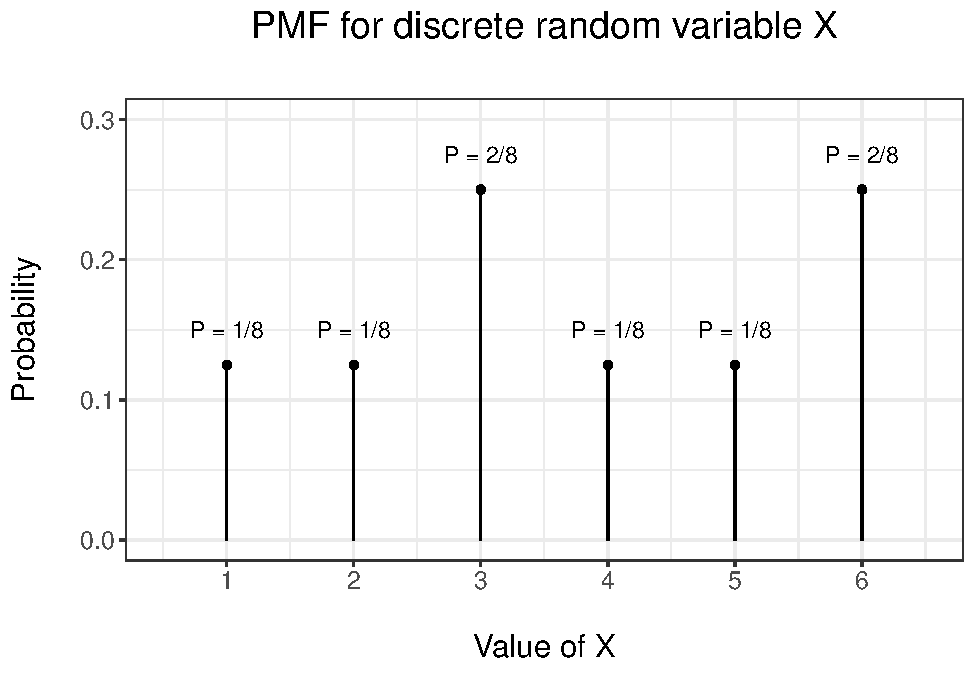
\includegraphics{SimBook_files/figure-latex/disc-pmf-1.pdf}
\caption{\label{fig:disc-pmf}PMF for the biased dice example}
\end{figure}

\hypertarget{cumulative-distribution-function}{%
\subsection{Cumulative Distribution Function}\label{cumulative-distribution-function}}

Whilst you should have been already familiar with the concept of pmf, the next concept may appear to be new. However, you have actually used it multiple times when computing Normal probabilities with the tables.

We now define what is usually called the \emph{cumulative distribution function} (or cdf) of a random variable \(X\). The cdf of \(X\) at the point \(x\in\mathbb{X}\) is
\[
F(x) = P(X \leq x) = \sum_{y \leq x} p(y)
\]
that is the probability that \(X\) is less or equal to \(x\) or equally the sum of the pmf of \(X\) for all values less than \(x\).

Let's consider the dice example to illustrate the idea of cdf and consider the following values \(x\):

\begin{itemize}
\item
  \(x=0\): we compute \(F(0) = P(X\leq 0 )= 0\) since \(X\) cannot take any values less or equal than zero;
\item
  \(x= 0.9\): we compute \(F(0.9)= P(X\leq 0.9) = 0\) using the same reasoning as before;
\item
  \(x = 1\): we compute \(F(1)= P(X\leq 1) = P(X=1) = 1/8\) since \(X\) can take the value 1 with probability 1/8;
\item
  \(x = 1.5\): we compute \(F(1.5) = P(X\leq 1.5) = P(X=1) = 1/8\) using the same reasoning as before;
\item
  \(x = 3.2\): we compute \(F(3.2)=P(X\leq 3.2)=P(X=1)+ P(X=2) + P(X=3)=1/8 + 1/8 + 2/8 = 0.5\) since \(X\) can take the values 1, 2 and 3 which are less than 3.2;
\end{itemize}

We can compute in a similar way the cdf for any value \(x\). A graphical visualization of the resulting CDF is given in Figure \ref{fig:disc-cdf}.

\begin{figure}
\centering
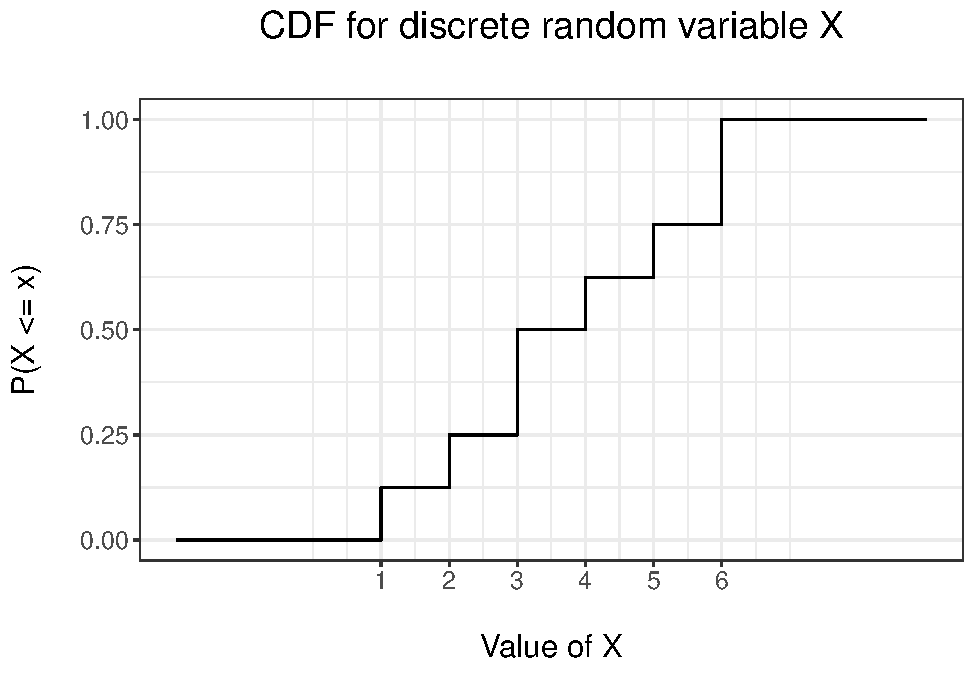
\includegraphics{SimBook_files/figure-latex/disc-cdf-1.pdf}
\caption{\label{fig:disc-cdf}CDF for the biased dice example}
\end{figure}

The plot highlights some properties of CDFs which can proved hold in general for any discrete CDF:

\begin{itemize}
\item
  it is a step function which is also non-decreasing;
\item
  on the left-hand-side it takes the value 0;
\item
  on the right-hand-side it takes the value 1.
\end{itemize}

\hypertarget{summaries}{%
\subsection{Summaries}\label{summaries}}

The pmf and the cdf fully characterize a discrete random variable \(X\). Often however we want to compress that information into a single number which still retains some aspect of the distribution of \(X\).

The \emph{expectation} or \emph{mean} of a random variable \(X\) denoted as \(E(X)\) is defined as
\[
E(X)=\sum_{x\in\mathbb{X}}xp(x)
\]
The expectation can be interpreted as the mean value of a large number of observations from the random variable \(X\). Consider again the example of the biased dice. The expectation is
\[
E(X)=1\cdot1/8 + 2\cdot1/8 + 3\cdot 2/8 + 4\cdot 1/8 + 5\cdot 1/8 + 6\cdot 2/8 = 3.75
\]
So if we were to throw the dice a large number of time, we would expect the average of the number shown to be 3.75.

The \emph{median} of the random variable \(X\) denoted as \(m(X)\) is defined as the value \(x\) such that \(P(X\leq x)\) is larger or equal to 0.5 and \(P(X\geq x)\) is larger or equal to 0.5. It is defined as the middle value of the distribution. For the dice example the median is the value 3: indeed \(P(X\leq 3 ) = P(X=1)+P(X=2)+P(X=3)=0.5 \geq 0.5\) and \(P(X\geq 3) = P(X=3) + P(X=4) + P(X=5) + P(X=6) = 0.75 \geq 0.5\).

The \emph{mode} of the random variable \(X\) is the value \(x\) such that \(p(x)\) is largest: it is the value of the random variable which is expected to happen most frequently. Notice that the mode may not be unique: in that case we say that the distribution of \(X\) is bimodal. The example of the biased dice as an instance of a bimodal distribution: the values 3 and 6 are the equally likely and they have the largest pmf.

The above three summaries are measures of \emph{centrality}: they describe the central tendency of \(X\). Next we consider measures of \emph{variability}: such measures will quantify the spread or the variation of the possible values of \(X\) around the mean.

The \emph{variance} of the discrete random variable \(X\) is the expectation of the squared difference between the random variable and its mean. Formally it is defined as
\[
V(X)=E((X-E(X))^2)=\sum_{x\in\mathbb{X}}(x-E(X))^2p(x)
\]
In general we will not compute variance by hand. The following R code computes the variance of the random variable associated to the biased dice.

\begin{Shaded}
\begin{Highlighting}[]
\NormalTok{x }\OtherTok{\textless{}{-}} \DecValTok{1}\SpecialCharTok{:}\DecValTok{6}  \CommentTok{\# outcomes of X}
\NormalTok{px }\OtherTok{\textless{}{-}} \FunctionTok{c}\NormalTok{(}\DecValTok{1}\SpecialCharTok{/}\DecValTok{8}\NormalTok{,}\DecValTok{1}\SpecialCharTok{/}\DecValTok{8}\NormalTok{,}\DecValTok{2}\SpecialCharTok{/}\DecValTok{8}\NormalTok{,}\DecValTok{1}\SpecialCharTok{/}\DecValTok{8}\NormalTok{,}\DecValTok{1}\SpecialCharTok{/}\DecValTok{8}\NormalTok{,}\DecValTok{2}\SpecialCharTok{/}\DecValTok{8}\NormalTok{)  }\CommentTok{\# pmf of X}
\NormalTok{Ex }\OtherTok{\textless{}{-}} \FunctionTok{sum}\NormalTok{(x}\SpecialCharTok{*}\NormalTok{px)  }\CommentTok{\# Expectation of X}
\NormalTok{Vx }\OtherTok{\textless{}{-}} \FunctionTok{sum}\NormalTok{((x}\SpecialCharTok{{-}}\NormalTok{Ex)}\SpecialCharTok{\^{}}\DecValTok{2}\SpecialCharTok{*}\NormalTok{px)  }\CommentTok{\# Variance of X}
\NormalTok{Vx}
\end{Highlighting}
\end{Shaded}

\begin{verbatim}
## [1] 2.9375
\end{verbatim}

The \emph{standard deviation} of the discrete random variable \(X\) is the square root of \(V(X)\).

\hypertarget{notable-discrete-variables}{%
\section{Notable Discrete Variables}\label{notable-discrete-variables}}

In the previous section we gave a generic definition of discrete random variables and discussed the conditions that a pmf must obey. We considered the example of a biased dice and constructed a pmf for that specific example.

There are situations that often happen in practice: for instance the case of experiments with binary outcomes. For such cases random variables with specific pmfs are given a name and their properties are well known and studied.

In this section we will consider three such distributions: Bernoulli, Binomial and Poisson.

\hypertarget{bernoulli-distribution}{%
\subsection{Bernoulli Distribution}\label{bernoulli-distribution}}

Consider an experiment or a real-world system where there can only be two outcomes:

\begin{itemize}
\item
  a toss of a coin: heads or tails;
\item
  the result of a COVID test: positive or negative;
\item
  the status of a machine: broken or working;
\end{itemize}

By default one outcome happens with some probability, that we denote as \(\theta\in [0,1]\) and the other with probability \(1-\theta\).

Such a situation is in general modeled using the so-called \emph{Bernoulli distribution} with parameter \(\theta\). One outcome is associated to the number 1 (usually referred to as sucess) and the other is associated to the number 0 (usually referred to as failure). So \(P(X=1)=p(1)=\theta\) and \(P(X=0)=p(0)=1-\theta\).

The above pmf can be more coincisely written as
\[
p(x)=\left\{
\begin{array}{ll}
\theta^x(1-\theta)^{1-x}, & x=0,1\\
0, & \mbox{otherwise}
\end{array}
\right.
\]
The mean and variance of the Bernoulli distribution can be easily computed as
\[
E(X)=0\cdot(1-\theta)+ 1\cdot\theta=\theta,
\]
and
\[
V(X)=(0-\theta)^2(1-\theta)+(1-\theta)^2\theta=\theta^2(1-\theta)+(1-\theta)^2\theta=\cdots = \theta(1-\theta)
\]

Figure \ref{fig:bernoulli} reports the pmf and the cdf of a Bernoulli random variable with parameter 0.3.

\begin{figure}
\centering
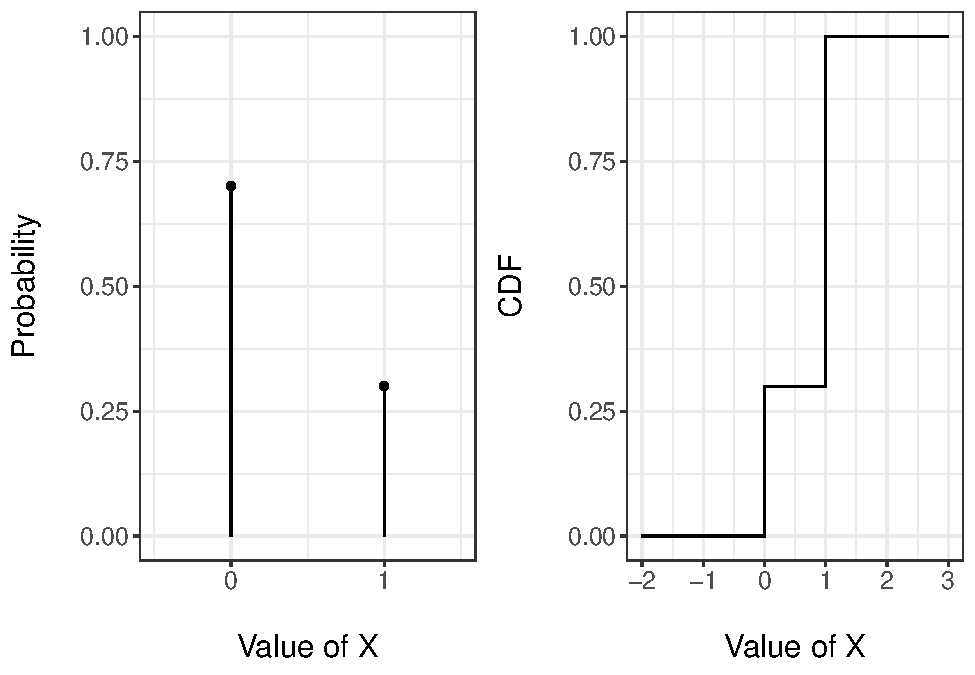
\includegraphics{SimBook_files/figure-latex/bernoulli-1.pdf}
\caption{\label{fig:bernoulli}PMF (left) and CDF (right) of a Bernoulli random variable with parameter 0.3}
\end{figure}

\hypertarget{binomial-distribution}{%
\subsection{Binomial Distribution}\label{binomial-distribution}}

The Bernoulli random variable is actually a very special case of the so-called \emph{Binomial} random variable. Consider experiments of the type discussed for Bernoullis: coin tosses, COVID tests etc. Now suppose that instead of having just one trial, each of these experiments are repeated multiple times. Consider the following assumptions:

\begin{itemize}
\item
  each experiment is repeated \(n\) times;
\item
  each time there is a probability of success \(\theta\);
\item
  the outcome of each experiment is independent of the others.
\end{itemize}

Let's think of tossing a coin \(n\) times. Then we would expect that the probability of showing heads is the same for all tosses and that the result of previous tosses does not affect others. So this situation appears to meet the above assumptions and can be modeled by what we call a Binomial random variable.

Formally, the random variable \(X\) is a Binomial random variable with parameters \(n\) and \(\theta\) if it denotes the number of successes of \(n\) independent Bernoulli random variables, all with parameter \(\theta\).

The pmf of a Binomial random variable with parameters \(n\) and \(\theta\) can be written as:
\[
p(x)=\left\{
\begin{array}{ll}
\binom{n}{x}\theta^{x}(1-\theta)^{n-x}, & x = 0,1,\dots,n\\
0, & \mbox{otherwise}
\end{array}
\right.
\]
Let's try and understand the formula by looking term by term.

\begin{itemize}
\item
  if \(X=x\) there are \(x\) successes and each success has probability \(\theta\) - so \(\theta^x\) counts the overall probability of successes
\item
  if \(X=x\) there are \(n-x\) failures and each failure has probability \(1-\theta\) - so \((1-\theta)^{n-x}\) counts the overall probability of failures
\item
  failures and successes can appear according to many orders. To see this, suppose that \(x=1\): there is only one success out of \(n\) trials. This could have been the first attempt, the second attempt or the \(n\)-th attempt. The term \(\binom{n}{x}\) counts all possible ways the outcome \(x\) could have happened.
\end{itemize}

The Bernoulli distribution can be seen as a special case of the Binomial where the parameter \(n\) is fixed to 1.

We will not show why this is the case but the expectation and the variance of the Binomial random variable with parameters \(n\) and \(\theta\) can be derived as
\[
E(X)=np, \hspace{2cm} V(X)=np(1-p)
\]
The formulae for the Bernoulli can be retrieved by setting \(n=1\).

Figure \ref{fig:binom} shows the pmf of two Binomial distributions both with parameter \(n=10\) and with \(\theta=0.3\) (left) and \(\theta=0.8\). For the case \(\theta=0.3\) we can see that it is more likely that there are a small number of successes, whilst for \(\theta=0.8\) a large number of successes is more likely.

\begin{figure}
\centering
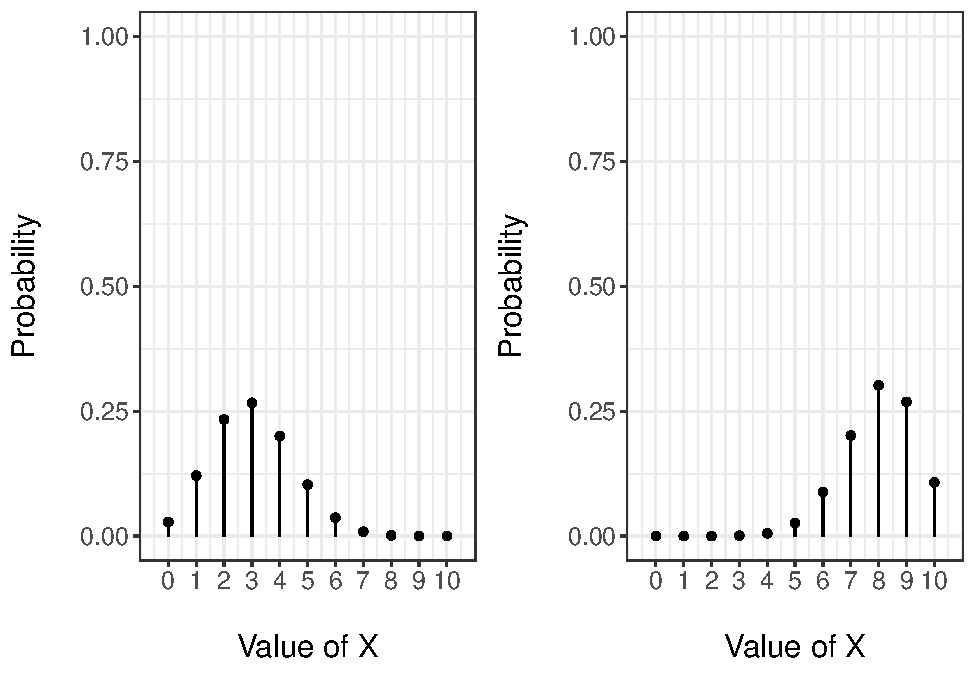
\includegraphics{SimBook_files/figure-latex/binom-1.pdf}
\caption{\label{fig:binom}PMF of a Binomial random variable with parameters n = 10 and theta = 0.3 (left) and theta = 0.8 (right)}
\end{figure}

R provides a straightforward implementation of the Binomial distribution through the functions \texttt{dbinom} for the pmf and \texttt{pbinom} for the cdf. They require three arguments:

\begin{itemize}
\item
  first argument is the value at which to compute the pmf or the cdf;
\item
  \texttt{size} is the parameter \(n\) of the Binomial;
\item
  \texttt{prob} is the parameter \(\theta\) of the Binomial.
\end{itemize}

So for instance

\begin{Shaded}
\begin{Highlighting}[]
\FunctionTok{dbinom}\NormalTok{(}\DecValTok{3}\NormalTok{, }\AttributeTok{size =} \DecValTok{10}\NormalTok{, }\AttributeTok{prob =} \FloatTok{0.5}\NormalTok{)}
\end{Highlighting}
\end{Shaded}

\begin{verbatim}
## [1] 0.1171875
\end{verbatim}

returns \(P(X=3)=p(3)\) for a Binomial random variable with parameter \(n=10\) and \(\theta = 0.5\).

Similarly,

\begin{Shaded}
\begin{Highlighting}[]
\FunctionTok{pbinom}\NormalTok{(}\DecValTok{8}\NormalTok{, }\AttributeTok{size =} \DecValTok{20}\NormalTok{, }\AttributeTok{prob =} \FloatTok{0.2}\NormalTok{)}
\end{Highlighting}
\end{Shaded}

\begin{verbatim}
## [1] 0.9900182
\end{verbatim}

returns \(P(X\leq 8) = F(8)\) for a Binomial random variable with parameter \(n=20\) and \(\theta = 0.2\).

\hypertarget{poisson-distribution}{%
\subsection{Poisson Distribution}\label{poisson-distribution}}

The last class of discrete random variables we discuss is the so-called \emph{Poisson} distribution. Whilst for Bernoulli and Binomial we had an interpretation of why the pmf took its specific form by associating it to independent binary experiments each with an equal probability of success, for the Poisson there is no such an interpretation.

A discrete random variable \(X\) has a Poisson distribution with parameter \(\lambda\) if its pmf is
\[
p(x)=\left\{
\begin{array}{ll}
\frac{e^{-\lambda}\lambda^x}{x!}, & x = 0,1,2,3,\dots\\
0, & \mbox{otherwise}
\end{array}
\right.
\]
where \(\lambda > 0\).

So the sample space of a Poisson random variable is the set of all non-negative integers.

One important characteristic of the Poisson distribution is that its mean and variance are equal to the parameter \(\lambda\), that is
\[
E(X)= V(X) = \lambda.
\]

Figure @ref\{fig:poisson\} gives an illustration of the form of the pmf of the Poisson distribution for two parameter choices: \(\lambda=1\) (left) and \(\lambda = 4\) (right). The x-axis is shown until \(x=10\) but recall that the Poisson is defined over all non-negative integers. For the case \(\lambda=1\) we can see that the outcomes 0 and 1 have the largest probability - recall that \(E(X)=0\). For the case \(\lambda = 4\) the outcomes \(x = 2,3,4,5\) have the largest probability.

\begin{figure}
\centering
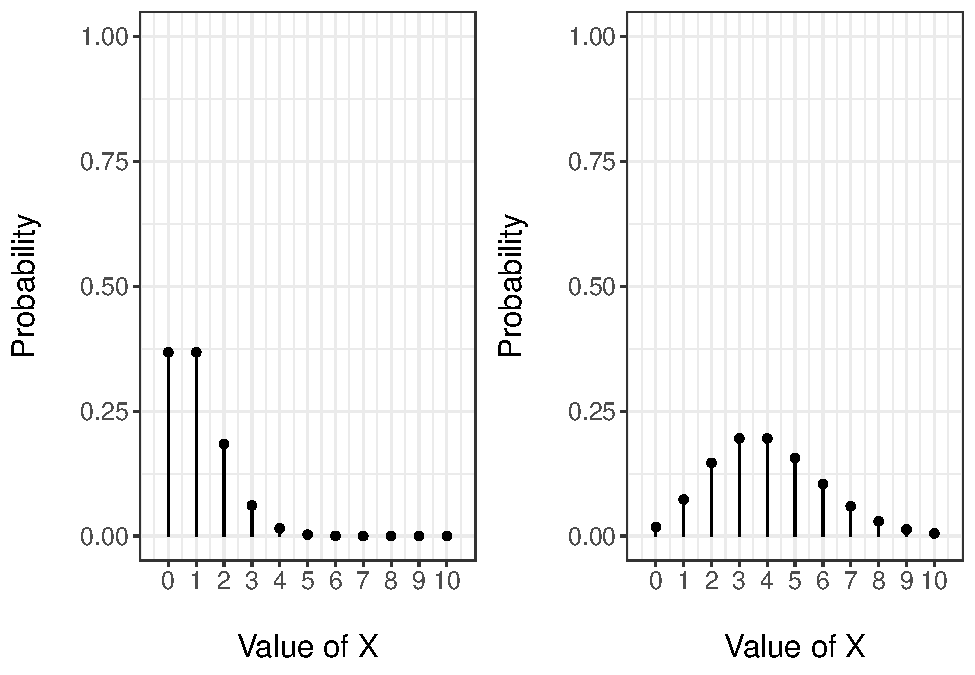
\includegraphics{SimBook_files/figure-latex/poisson-1.pdf}
\caption{\label{fig:poisson}PMF of a Poisson random variable with parameter 1 (left) and 4 (right)}
\end{figure}

R provides a straightforward implementation of the Poisson distribution through the functions \texttt{dpois} for the pmf and \texttt{ppois} for the cdf. They require three arguments:

\begin{itemize}
\item
  first argument is the value at which to compute the pmf or the cdf;
\item
  \texttt{lambda} is the parameter \(\lambda\) of the Poisson;
\end{itemize}

So for instance

\begin{Shaded}
\begin{Highlighting}[]
\FunctionTok{dpois}\NormalTok{(}\DecValTok{3}\NormalTok{, }\AttributeTok{lambda =} \DecValTok{1}\NormalTok{)}
\end{Highlighting}
\end{Shaded}

\begin{verbatim}
## [1] 0.06131324
\end{verbatim}

returns \(P(X=3)=p(3)\) for a Poisson random variable with parameter \(\lambda = 1\).

Similarly,

\begin{Shaded}
\begin{Highlighting}[]
\FunctionTok{ppois}\NormalTok{(}\DecValTok{8}\NormalTok{, }\AttributeTok{lambda =} \DecValTok{4}\NormalTok{)}
\end{Highlighting}
\end{Shaded}

\begin{verbatim}
## [1] 0.9786366
\end{verbatim}

returns \(P(X\leq 8) = F(8)\) for a Poisson random variable with parameter \(\lambda = 4\).

\hypertarget{some-examples}{%
\subsection{Some Examples}\label{some-examples}}

We next consider two examples to see in practice the use of the Binomial and Poisson distributions.

\hypertarget{probability-of-marriage}{%
\subsubsection{Probability of Marriage}\label{probability-of-marriage}}

A recent survey indicated that 82\% of single women aged 25 years old will be married in their lifetime. Compute

\begin{itemize}
\item
  the probability of at most 3 women will be married in a sample of 20;
\item
  the probability of at least 90 women will be married in sample of 100;
\item
  the probability of two or three women in a sample of 20 will never be married.
\end{itemize}

The above situation can be modeled by a Binomial random variable where the parameter \(n\) depends on the question and \(\theta = 0.82\).

The first question requires us to compute \(P(X\leq 3)= F(3)\) where \(X\) is Binomial with parameters \(n=20\) and \(\theta =0.82\). Using R

\begin{Shaded}
\begin{Highlighting}[]
\FunctionTok{pbinom}\NormalTok{(}\DecValTok{3}\NormalTok{, }\AttributeTok{size =} \DecValTok{10}\NormalTok{, }\AttributeTok{prob =} \FloatTok{0.82}\NormalTok{)}
\end{Highlighting}
\end{Shaded}

\begin{verbatim}
## [1] 0.0004400767
\end{verbatim}

The second question requires us to compute \(P(X\geq 90)\) where \(X\) is a Binomial random variable with parameters \(n=100\) and \(\theta = 0.82\). Notice that
\[
P(X\geq 90) = 1 - P(X< 90) = 1 - P(X\leq 89) = 1 - F(89).
\]
Using R

\begin{Shaded}
\begin{Highlighting}[]
\DecValTok{1} \SpecialCharTok{{-}} \FunctionTok{pbinom}\NormalTok{(}\DecValTok{89}\NormalTok{, }\AttributeTok{size =} \DecValTok{100}\NormalTok{,  }\AttributeTok{prob =} \FloatTok{0.82}\NormalTok{)}
\end{Highlighting}
\end{Shaded}

\begin{verbatim}
## [1] 0.02003866
\end{verbatim}

For the third question, notice that saying two women out of 20 will never be married is equal to 18 out of 20 will be married. Therefore we need to compute \(P(X=17) + P(X=18)= p(17) + p(18)\) where \(X\) is a Binomial random variable with parameters \(n=20\) and \(\theta = 0.82\). Using R

\begin{Shaded}
\begin{Highlighting}[]
\FunctionTok{sum}\NormalTok{(}\FunctionTok{dbinom}\NormalTok{(}\DecValTok{17}\SpecialCharTok{:}\DecValTok{18}\NormalTok{, }\AttributeTok{size =} \DecValTok{20}\NormalTok{, }\AttributeTok{prob =} \FloatTok{0.82}\NormalTok{))}
\end{Highlighting}
\end{Shaded}

\begin{verbatim}
## [1] 0.4007631
\end{verbatim}

\hypertarget{the-bad-stuntman}{%
\subsubsection{The Bad Stuntman}\label{the-bad-stuntman}}

A stuntman injures himself an average of three times a year. Use the Poisson probability formula to calculate the probability that he will be injured:

\begin{itemize}
\item
  4 times a year
\item
  Less than twice this year.
\item
  More than three times this year.
\end{itemize}

The above situation can be modeled as a Poisson distribution \(X\) with parameter \(\lambda = 3\).

The first question requires us to compute \(P(X=4)\) which using R can be computed as

\begin{Shaded}
\begin{Highlighting}[]
\FunctionTok{dpois}\NormalTok{(}\DecValTok{4}\NormalTok{, }\AttributeTok{lambda =}\DecValTok{3}\NormalTok{)}
\end{Highlighting}
\end{Shaded}

\begin{verbatim}
## [1] 0.1680314
\end{verbatim}

The second question requires us to compute \(P(X<2) = P(X=0)+P(X=1)= F(1)\) which using R can be computed as

\begin{Shaded}
\begin{Highlighting}[]
\FunctionTok{ppois}\NormalTok{(}\DecValTok{1}\NormalTok{,}\AttributeTok{lambda=}\DecValTok{3}\NormalTok{)}
\end{Highlighting}
\end{Shaded}

\begin{verbatim}
## [1] 0.1991483
\end{verbatim}

The third question requires us to compute \(P(X>3) = 1 - P(X\leq 2) = 1 - F(2)\) which using R can be computed as

\begin{Shaded}
\begin{Highlighting}[]
\DecValTok{1} \SpecialCharTok{{-}} \FunctionTok{ppois}\NormalTok{(}\DecValTok{2}\NormalTok{, }\AttributeTok{lambda =} \DecValTok{3}\NormalTok{)}
\end{Highlighting}
\end{Shaded}

\begin{verbatim}
## [1] 0.5768099
\end{verbatim}

\hypertarget{continuous-random-variables}{%
\section{Continuous Random Variables}\label{continuous-random-variables}}

Our attention now turns to continuous random variables. These are in general more technical and less intuitive than discrete ones. You should not worry about all the technical details, since these are in general not important, and focus on the interpretation.

A continuous random variable \(X\) is a random variable whose sample space \(\mathbb{X}\) is an interval or a collection of intervals. In general \(\mathbb{X}\) may coincide with the set of real numbers \(\mathbb{R}\) or some subset of it. Examples of continuous random variables:

\begin{itemize}
\item
  the pressure of a tire of a car: it can be any positive real number;
\item
  the current temperature in the city of Madrid: it can be any real number;
\item
  the height of the students of Simulation and Modeling to understand change: it can be any real number.
\end{itemize}

Whilst for discrete random variables we considered summations over the elements of \(\mathbb{X}\), i.e.~\(\sum_{x\in\mathbb{X}}\), for continuous random variables we need to consider integrals over appropriate intervals.

You should be more or less familiar with these from previous studies of calculus. But let's give an example. Consider the function \(f(x)=x^2\) computing the squared of a number \(x\). Suppose we are interested in this function between the values -1 and 1, which is plotted by the red line in Figure \ref{fig:x-sq}. Consider the so-called integral \(\int_{-1}^{1}x^2dx\): this coincides with the area delimited by the function and the x-axis. In Figure \ref{fig:x-sq} the blue area is therefore equal to \(\int_{-1}^{1}x^2dx\).

\begin{figure}

{\centering 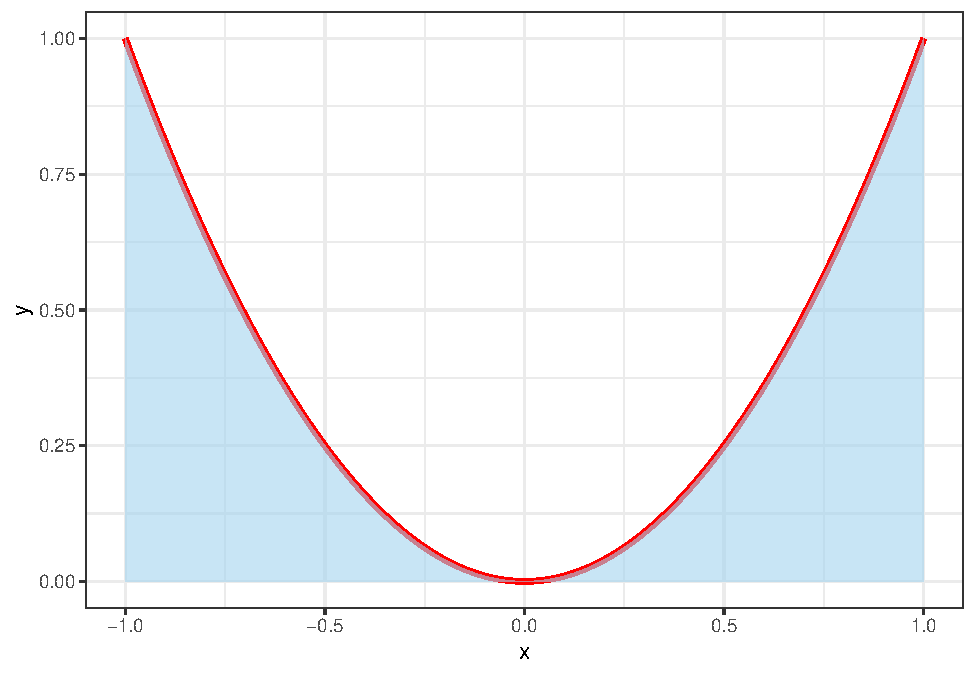
\includegraphics[width=0.5\linewidth]{SimBook_files/figure-latex/x-sq-1} 

}

\caption{Plot of the squared function and the area under its curve}\label{fig:x-sq}
\end{figure}

We will not be interested in computing integrals ourselves, so if you do not know/remember how to do it, there is no problem!

\hypertarget{probability-density-function}{%
\subsection{Probability Density Function}\label{probability-density-function}}

Discrete random variable are easy to work with in the sense that there exists a function, that we called probability mass function, such that \(p(x)=P(X=x)\), that is the value of that function in the point \(x\) is exactly the probability that \(X=x\).

Therefore we may wonder if this is true for a continuous random variable too. Sadly, the answer is no and probabilities for continuous random variables are defined in a slightly more involved way.

Let \(X\) be a continuous random variable with sample space \(\mathbb{X}\). The probability that \(X\) takes values in the interval \([a,b]\) is given by
\[
P(a\leq X \leq b) = \int_{a}^bf(x)dx
\]
where \(f(x)\) is called the \emph{probability density function} (pdf in short). Pdfs, just like pmfs must obey two conditions:

\begin{itemize}
\item
  \(f(x)\geq 0\) for all \(x\in\mathbb{X}\);
\item
  \(\int_{x\in\mathbb{X}}f(x)dx=1\).
\end{itemize}

So in the discrete case the pmf is defined exactly as the probability. In the continuous case the pdf is the function such that its integral is the probability that random variable takes values in a specific interval.

As a consequence of this definition notice that for any specific value \(x_0\in\mathbb{X}\), \(P(X=x_0)=0\) since
\[
\int_{x_0}^{x_0}f(x)dx = 0.
\]

Let's consider an example. The waiting time of customers of a donuts shop is believed to be random and to follow a random variable whose pdf is
\[
f(x) = \left\{
\begin{array}{ll}
\frac{1}{4}e^{-x/4}, & x\geq 0\\
0, & \mbox{otherwise}
\end{array}
\right.
\]

The pdf is drawn in Figure \ref{fig:exp} by the red line. One can see that \(f(x)\geq 0\) for all \(x\geq 0\) and one could also compute that it integrates to one.

Therefore the probability that the waiting time is between any two values \((a,b)\) can be computed as
\[
\int_a^b\frac{1}{4}e^{-x/4}dx.
\]
In particular if we were interested in the probability that the waiting time is between two and five minutes, corresponding to the shaded area in Figure \ref{fig:exp}, we could compute it as
\[
P(2<X<5)=\int_2^5f(x)dx=\int_{2}^5\frac{1}{4}e^{-x/4}dx= 0.32
\]

\begin{figure}

{\centering 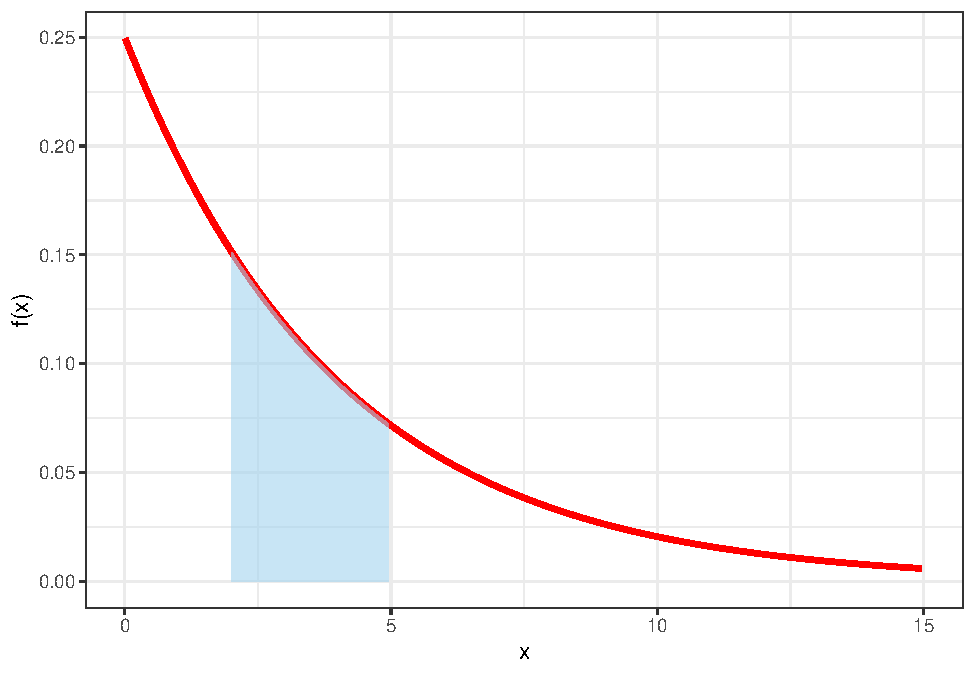
\includegraphics[width=0.5\linewidth]{SimBook_files/figure-latex/exp-1} 

}

\caption{Probability density function for the waiting time in the donut shop example}\label{fig:exp}
\end{figure}

Notice that since \(P(X=x_0)=0\) for any \(x_0\in\mathbb{X}\), we also have that
\[
P(a\leq X \leq b)=P(a < X \leq b) = P(a\leq X < b) = P(a<X<b).
\]

\hypertarget{cumulative-distribution-function-1}{%
\subsection{Cumulative Distribution Function}\label{cumulative-distribution-function-1}}

For a continuous random variable \(X\) the cumulative distribution function (cdf) is equally defined as
\[
F(x) = P(X \leq x),
\]
where now
\[
P(X \leq x) = P(X < x) = \int_{-\infty}^xf(t)dt.
\]
so the summation is substituted by an integral.

Let's consider again the donut shop example as an illustration. The cdf is defined as
\[
F(x)=\int_{-\infty}^xf(t)dt = \int_{-\infty}^x\frac{1}{4}e^{-x/4}.
\]
This integral can be solved and \(F(x)\) can be calculated as
\[
F(x)= 1- e^{-x/4},
\]
which is plotted in Figure \ref{fig:expcdf}.

\begin{figure}

{\centering 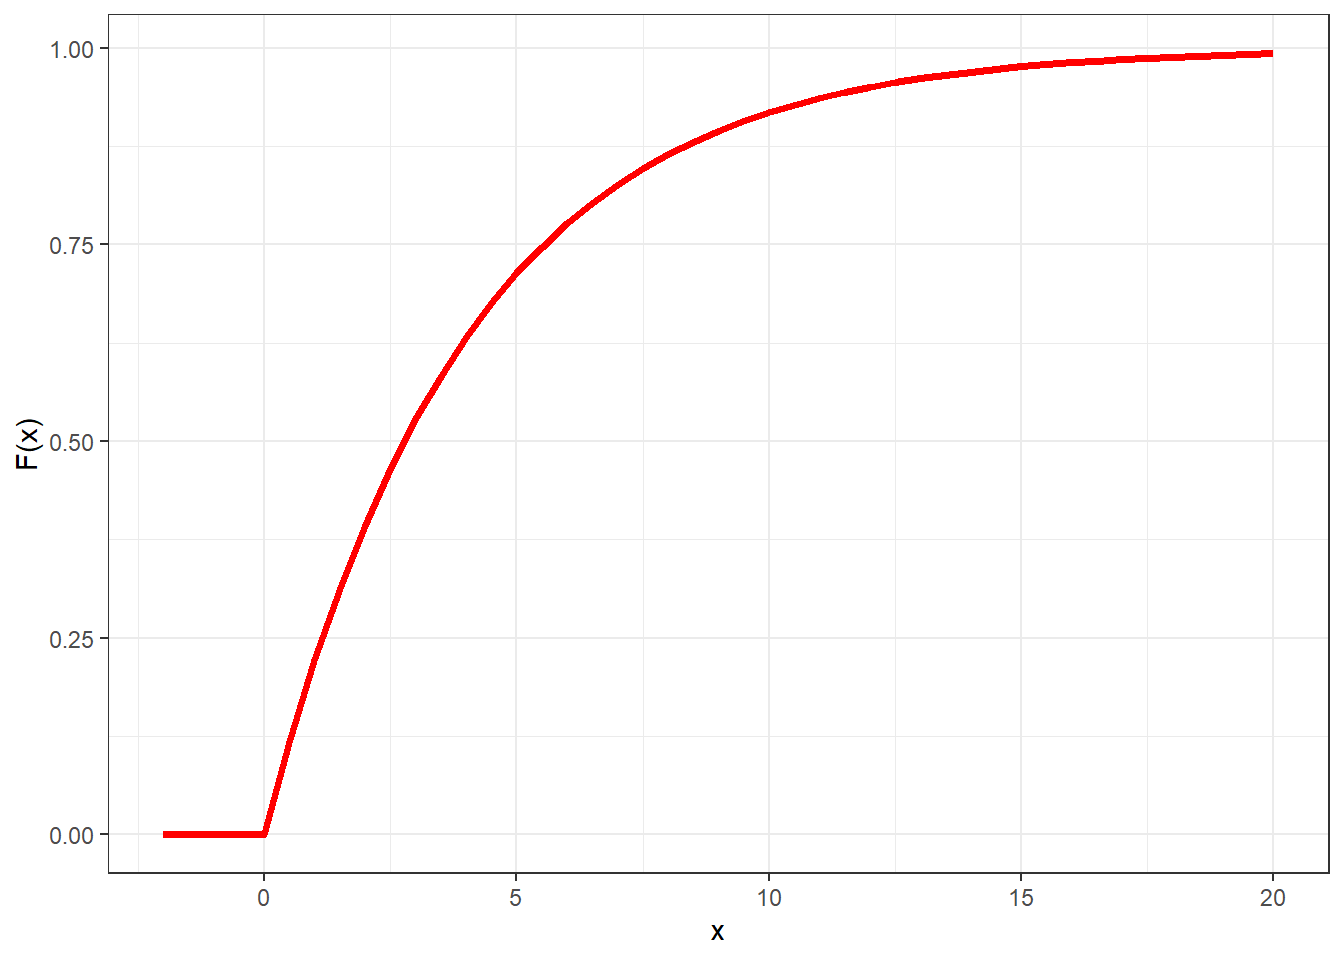
\includegraphics[width=0.5\linewidth]{SimBook_files/figure-latex/expcdf-1} 

}

\caption{Cumulative distribution function for the waiting time at the donut shop}\label{fig:expcdf}
\end{figure}

We can notice that the cdf has similar properties as in the discrete case: it is non-decreasing, on the left-hand side is zero and on the right-hand side tends to zero.

In the continuous case, one can prove that cdfs and pdfs are related as
\[
f(x)=\frac{d}{dx}F(x).
\]

\hypertarget{summaries-1}{%
\subsection{Summaries}\label{summaries-1}}

Just as for discrete random variables, we may want to summarize some features of a continuous random variable into a unique number. The same set of summaries exists for continuous random variables, which are almost exactly defined as in the discrete case (integrals are used instead of summations).

\begin{itemize}
\item
  \emph{mean}: the mean of a continuous random variable \(X\) is defined as
  \[
   E(X) = \int_{-\infty}^{+\infty}xf(x)dx
   \]
\item
  \emph{median}: the median of a continuous random variable \(X\) is defined as the value \(x\) such that \(P(X\leq x) = 0.5\) or equally \(F(x)=0.5\).
\item
  \emph{mode}: the mode of a continuous random variable \(X\) is defined the value \(x\) such that \(f(x)\) is largest.
\item
  \emph{variance}: the variance of a continuous random variable \(X\) is defined as
  \[
   V(X)=\int_{-\infty}^{+\infty}(x-E(X))^2f(x)dx
   \]
\item
  \emph{standard deviation}: the standard deviation of a continuous random variable \(X\) is defined as \(\sqrt{V(X)}\).
\end{itemize}

\hypertarget{notable-continuous-distribution}{%
\section{Notable Continuous Distribution}\label{notable-continuous-distribution}}

As in the discrete case, there are some types of continuous random variables that are used frequently and therefore are given a name and their proprieties are well-studied.

\hypertarget{uniform-distribution}{%
\subsection{Uniform Distribution}\label{uniform-distribution}}

The first, and simplest, continuous random variable we study is the so-called (continuous) \emph{uniform} distribution. We say that a random variable \(X\) is uniformly distributed on the interval \([a,b]\) if its pdf is
\[
f(x)=\left\{ 
\begin{array}{ll}
\frac{1}{b-a}, & a\leq x \leq b\\
0, & \mbox{otherwise} 
\end{array}
\right.
\]
This is plotted in Figure \ref{fig:unipdf} for choices of parameters \(a=2\) and \(b=6\)

\begin{figure}

{\centering 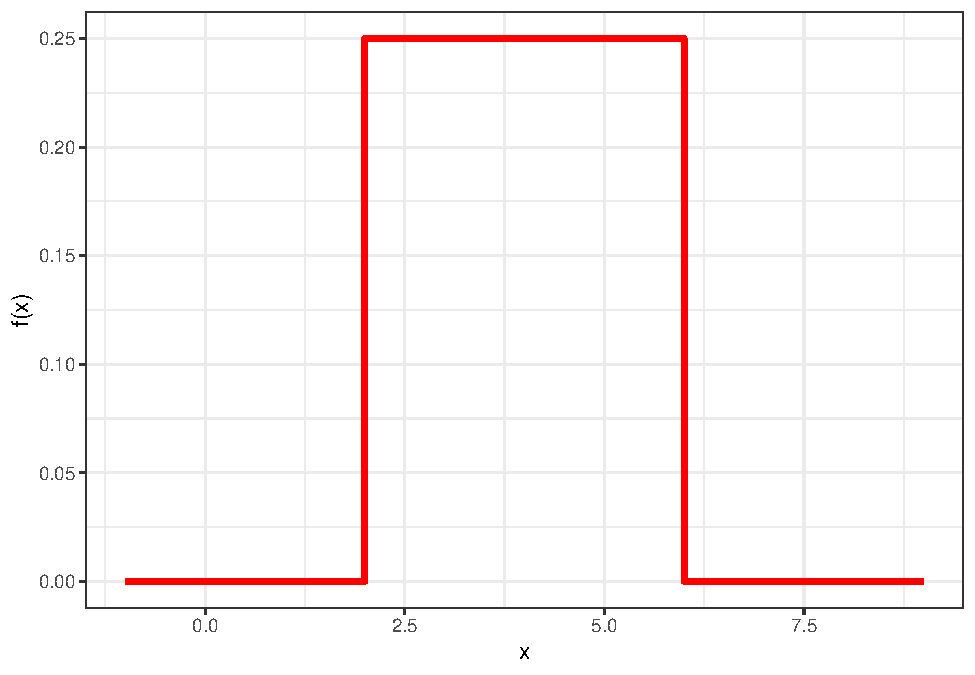
\includegraphics[width=0.5\linewidth]{SimBook_files/figure-latex/unipdf-1} 

}

\caption{Probability density function for a uniform random variable with parameters a = 2 and b = 6}\label{fig:unipdf}
\end{figure}

By looking at the pdf we see that it is a flat, constant line between the values \(a\) and \(b\). This implies that the probability that \(X\) takes values between two values \(x_0\) and \(x_1\) only dependens on the length of the interval \((x_0,x_1)\).

Its cdf can be derived as
\[
F(x)=\left\{
\begin{array}{ll}
0, & x<a\\
\frac{x-a}{b-a}, & a\leq x \leq b\\
1, & x>b
\end{array}
\right.
\]
and this is plotted in Figure \ref{fig:unicdf}.

\begin{figure}

{\centering 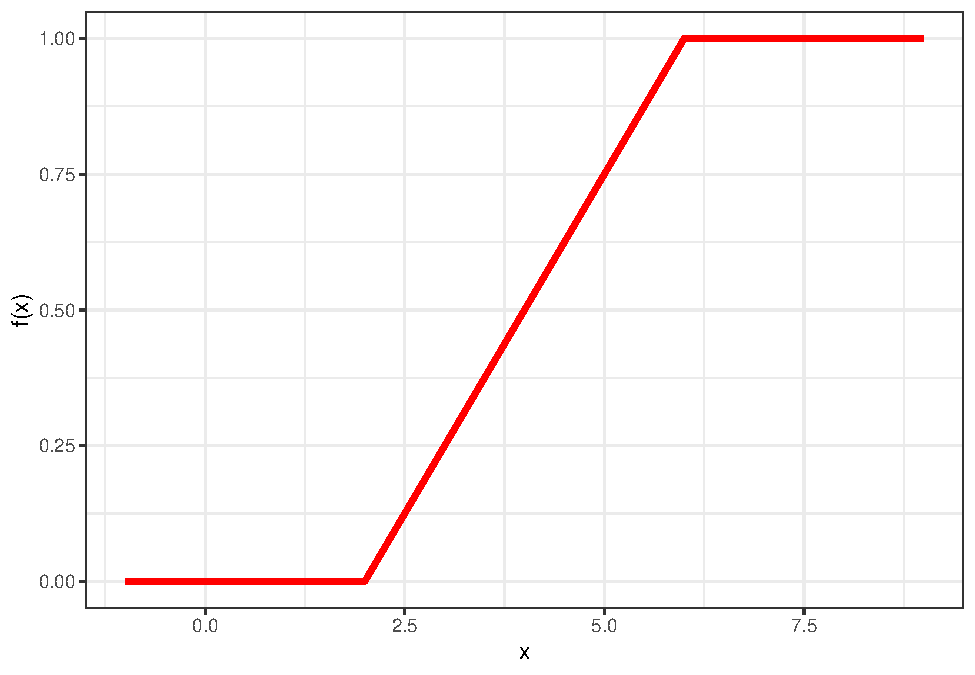
\includegraphics[width=0.5\linewidth]{SimBook_files/figure-latex/unicdf-1} 

}

\caption{Cumulative distribution function for a uniform random variable with parameters a = 2 and b = 6}\label{fig:unicdf}
\end{figure}

The mean and variance of a uniform can be derived as
\[
E(X)=\frac{a+b}{2}, \hspace{1cm} V(X)=\frac{(b-a)^2}{12}.
\]
So the mean is equal to the middle point of the interval \((a,b)\).

The uniform distribution will be fundamental in simulation. We will see that the starting point to simulate random numbers from any distribution will require the simulation of random numbers uniformly distributed between 0 and 1.

R provides an implementation of the uniform random variable with the functions \texttt{dunif} and \texttt{punif} whose details are as follows:

\begin{itemize}
\item
  the first argument is the value at which to compute the function;
\item
  the second argument, \texttt{min}, is the parameter \(a\), by default equal to zero;
\item
  the third argument, \texttt{max}, is the parameter \(b\), by default equal to one.
\end{itemize}

So for instance

\begin{Shaded}
\begin{Highlighting}[]
\FunctionTok{dunif}\NormalTok{(}\DecValTok{5}\NormalTok{, }\AttributeTok{min =} \DecValTok{2}\NormalTok{, }\AttributeTok{max =} \DecValTok{6}\NormalTok{)}
\end{Highlighting}
\end{Shaded}

\begin{verbatim}
## [1] 0.25
\end{verbatim}

computes the pdf at the point 5 of a uniform random variable with parameters \(a=2\) and \(b=6\).

Conversely,

\begin{Shaded}
\begin{Highlighting}[]
\FunctionTok{punif}\NormalTok{(}\FloatTok{0.5}\NormalTok{)}
\end{Highlighting}
\end{Shaded}

\begin{verbatim}
## [1] 0.5
\end{verbatim}

computes the cdf at the point 0.5 of a uniform random variable with parameters \(a=0\) and \(b=1\).

\hypertarget{exponential-distribution}{%
\subsection{Exponential Distribution}\label{exponential-distribution}}

The second class of continuous random variables we will study are the so-called \emph{exponential} random variables. We have actually already seen such a random variable in the donut shop example. More generally, we say that a continuous random variable \(X\) is exponential with parameter \(\lambda>0\) if its pdf is
\[
f(x) = \left\{
\begin{array}{ll}
\lambda e^{-\lambda x}, & x\geq 0\\
0, & \mbox{otherwise}
\end{array}
\right.
\]

Figure \ref{fig:exppdf1} reports the pdf of exponential random variables for various choices of the parameter \(\lambda\).

\begin{figure}

{\centering 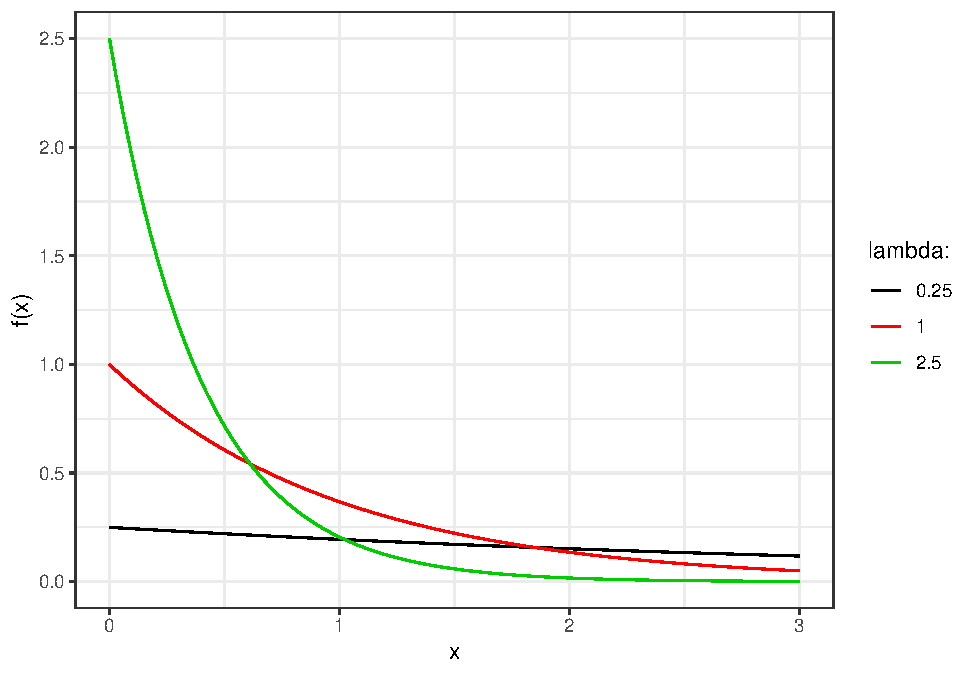
\includegraphics[width=0.5\linewidth]{SimBook_files/figure-latex/exppdf1-1} 

}

\caption{Probability density function for exponential random variables}\label{fig:exppdf1}
\end{figure}

Exponential random variables are very often used in dynamic simulations since they are very often used to model interarrival times in process: for instance the time between arrivals of customers at the donut shop.

Its cdf can be derived as
\[
F(x)=\left\{
\begin{array}{ll}
0, & x <0\\
1-e^{-\lambda x}, & x\geq 0
\end{array}
\right.
\]
and is reported in Figure \ref{fig:expcdf1} for the same choices of parameters.

\begin{figure}

{\centering 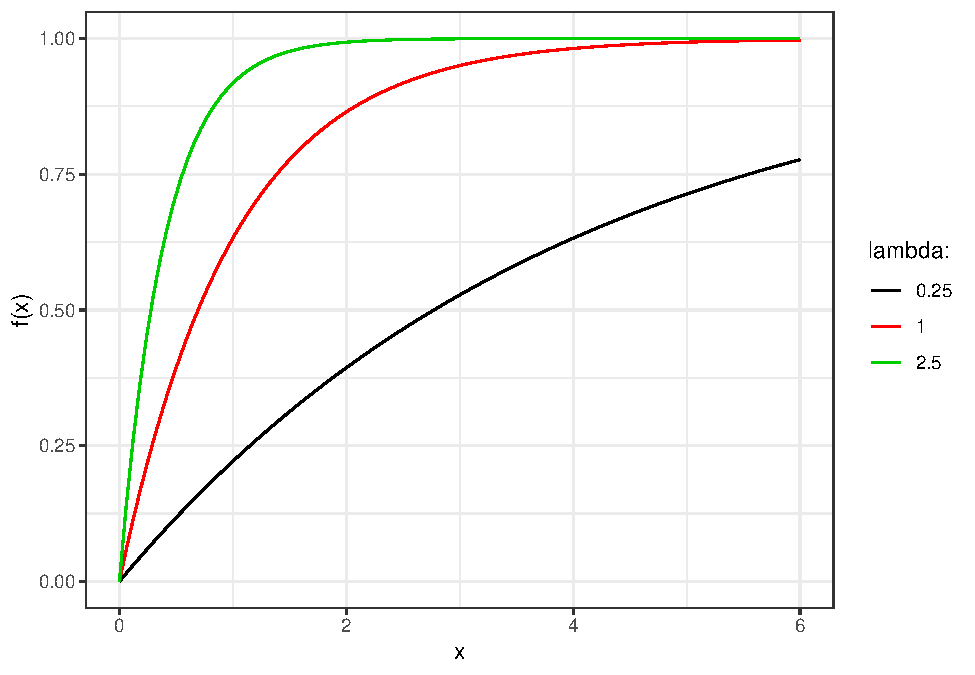
\includegraphics[width=0.5\linewidth]{SimBook_files/figure-latex/expcdf1-1} 

}

\caption{Cumulative distribution function for exponential random variables}\label{fig:expcdf1}
\end{figure}

The mean and the variance of exponential random variables can be computed as

\[
E(X)=\frac{1}{\lambda}, \hspace{1cm} V(X)=\frac{1}{\lambda^2}
\]

R provides an implementation of the uniform random variable with the functions \texttt{dexp} and \texttt{pexp} whose details are as follows:

\begin{itemize}
\item
  the first argument is the value at which to compute the function;
\item
  the second argument, \texttt{rate}, is the parameter \(\lambda\), by default equal to one;
\end{itemize}

So for instance

\begin{Shaded}
\begin{Highlighting}[]
\FunctionTok{dexp}\NormalTok{(}\DecValTok{2}\NormalTok{, }\AttributeTok{rate =} \DecValTok{3}\NormalTok{)}
\end{Highlighting}
\end{Shaded}

\begin{verbatim}
## [1] 0.007436257
\end{verbatim}

computes the pdf at the point 2 of an exponential random variable with parameter \(\lambda =3\).

Conversely

\begin{Shaded}
\begin{Highlighting}[]
\FunctionTok{pexp}\NormalTok{(}\DecValTok{4}\NormalTok{)}
\end{Highlighting}
\end{Shaded}

\begin{verbatim}
## [1] 0.9816844
\end{verbatim}

computes the cdf at the point 4 of an exponential random variable with parameter \(\lambda =1\).

\hypertarget{normal-distribution}{%
\subsection{Normal Distribution}\label{normal-distribution}}

The last class of continuous random variables we consider is the so-called \emph{Normal} or \emph{Gaussian} random variable. They are the most used and well-known random variable in statistics and we will see why this is the case.

A continuous random variable \(X\) is said to have a Normal distribution with mean \(\mu\) and variance \(\sigma^2\) if its pdf is
\[
f(x) = \frac{1}{\sqrt{2\pi\sigma^2}}\exp\left(-\frac{1}{2}\frac{(x-\mu)^2}{\sigma^2}\right).
\]
Recall that
\[
E(X)=\mu, \hspace{1cm} V(X)=\sigma^2,
\]
and so the parameters have a straightforward interpretation in terms of mean and variance.

Figure \ref{fig:norm} shows the form of the pdf of the Normal distribution for various choices of the parameters. On the left we have Normal pdfs for \(\sigma^2=1\) and various choices of \(\mu\): we can see that \(\mu\) shifts the plot on the x-axis. On the right we have Normal pdfs for \(\mu=1\) and various choices of \(\sigma^2\): we can see that all distributions are centered around the same value while they have a different spread/variability.

\begin{figure}

{\centering 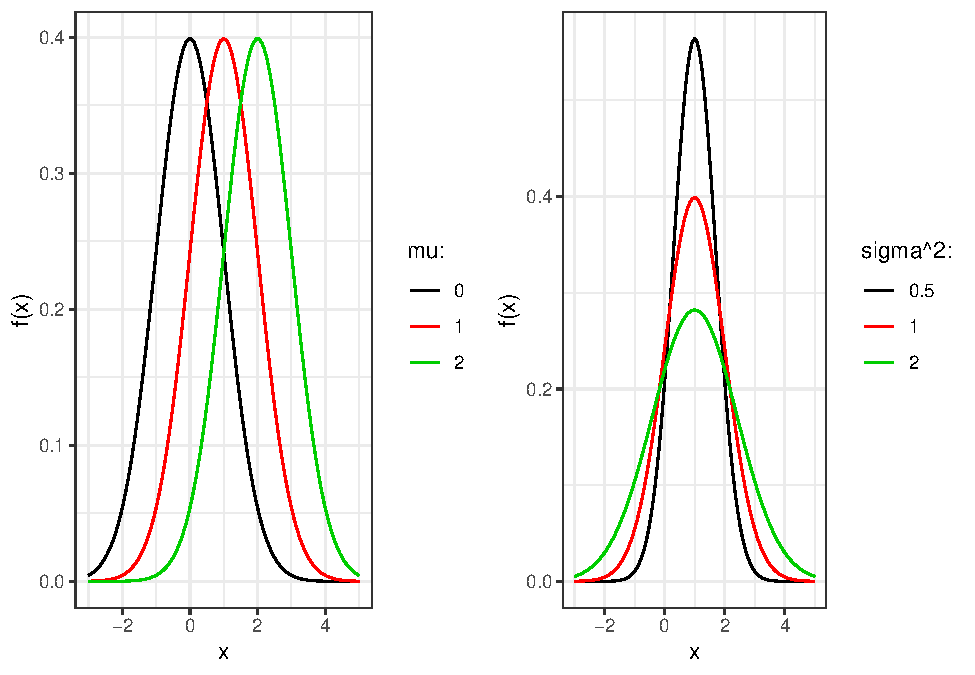
\includegraphics[width=0.5\linewidth]{SimBook_files/figure-latex/norm-1} 

}

\caption{Probability density function for normal random variables}\label{fig:norm}
\end{figure}

The form of the Normal pdf is the well-known so-called bell-shaped function. We can notice some properties:

\begin{itemize}
\item
  it is symmetric around the mean: the function on the left-hand side and on the right-hand side of the mean is mirrored. This implies that the median is equal to the mean ;
\item
  the maximum value of the pdf occurs at the mean. This implies that the mode is equal to the mean (and therefore also the median).
\end{itemize}

The cdf of the Normal random variable with parameters \(\mu\) and \(\sigma^2\) is
\[
F(x) = P(X\leq x)=\int_{-\infty}^{+\infty}\frac{1}{\sqrt{2\pi\sigma^2}}\exp\left(-\frac{1}{2}\frac{(x-\mu)^2}{\sigma^2}\right)dx
\]

The cdf of the Normal for various choices of parameters is reported in Figure \ref{fig:pnorm}.

\begin{figure}

{\centering 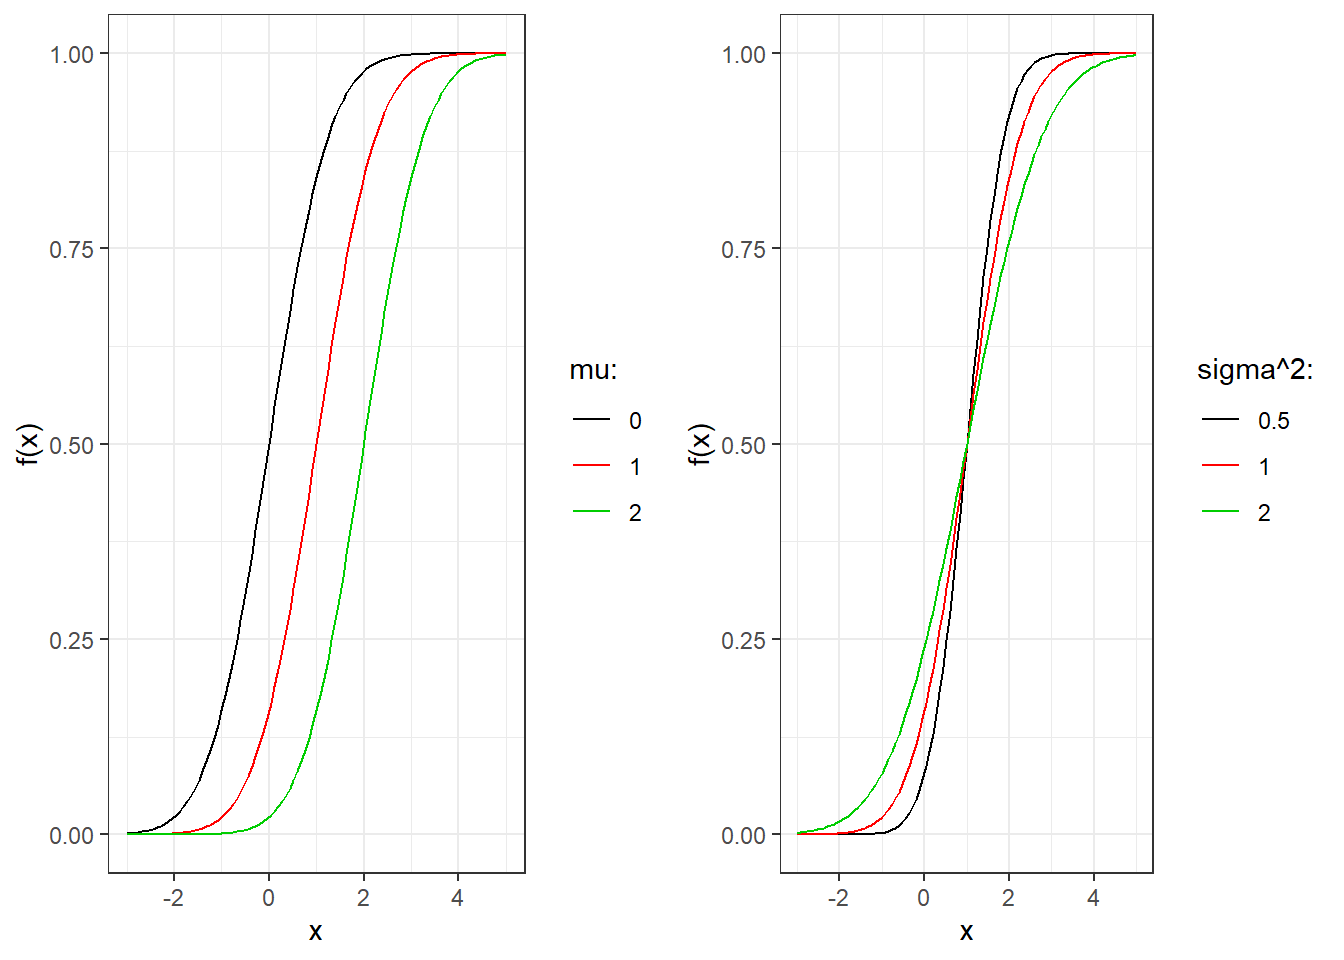
\includegraphics[width=0.5\linewidth]{SimBook_files/figure-latex/pnorm-1} 

}

\caption{Cumulative distribution function for normal random variables}\label{fig:pnorm}
\end{figure}

Unfortunately it is not possible to solve such an integral (as for example for the Uniform and the Exponential), and in general it is approximated using some numerical techniques. This is surprising considering that the Normal distribution is so widely used!!!

However, notice that we would need to compute such an approximation for every possible value of \((\mu,\sigma^2)\), depending on the distribution we want to use. This is unfeasible to do in practice.

There is a trick here, that you must have used multiple times already. We can transform a Normal \(X\) with parameters \(\mu\) and \(\sigma^2\) to the so-called \emph{standard Normal} random variable \(Z\), and viceversa, using the relationship:
\begin{equation}
 \label{eq:standard}
Z = \frac{X-\mu}{\sigma}, \hspace{1cm} X= \mu + \sigma Z.
\end{equation}
It can be shown that \(Z\) is a Normal random variable with parameter \(\mu=0\) and \(\sigma^2=1\).

The values of the cdf of the standard Normal random variable then need to be computed only once since \(\mu\) and \(\sigma^2\) are fixed. You have seen these numbers many many times in what are usually called the tables of the Normal distribution.

As a matter of fact you have also computed many times the cdf of a generic Normal random variable. First you computed \(Z\) using equation \eqref{eq:standard} and then looked at the Normal tables to derive that number.

Let's give some details about the standard Normal. Its pdf is
\[
\phi(z)=\frac{1}{\sqrt{2\pi}}\exp\left(-z^2/2\right).
\]
It can be seen that it is the same as the one of the Normal by setting \(\mu=0\) and \(\sigma^2=1\). Such a function is so important that it is given its own symbol \(\phi\).

The cdf is
\[
\Phi(z)=\int_{-\infty}^z\frac{1}{\sqrt{2\pi}}\exp\left(-x^2/2\right)dx
\]
Again this cannot be computed exactly, there is no closed-form expression. This is why you had to look at the tables instead of using a simple formula. The cdf of the standard Normal is also so important that it is given its own symbol \(\phi\).

Instead of using the tables, we can use R to tell us the values of Normal probabilities. R provides an implementation of the Normal random variable with the functions \texttt{dnorm} and \texttt{pnorm} whose details are as follows:

\begin{itemize}
\item
  the first argument is the value at which to compute the function;
\item
  the second argument, \texttt{mean}, is the parameter \(\mu\), by default equal to zero;
\item
  the third argument, \texttt{sd}, is the standard deviation, that is \(\sqrt{\sigma^2}\), by default equal to one.
\end{itemize}

So for instance

\begin{Shaded}
\begin{Highlighting}[]
\FunctionTok{dnorm}\NormalTok{(}\DecValTok{3}\NormalTok{)}
\end{Highlighting}
\end{Shaded}

\begin{verbatim}
## [1] 0.004431848
\end{verbatim}

computes the value of the standard Normal pdf at the value three.

Similarly,

\begin{Shaded}
\begin{Highlighting}[]
\FunctionTok{pnorm}\NormalTok{(}\FloatTok{0.4}\NormalTok{,}\DecValTok{1}\NormalTok{,}\FloatTok{0.5}\NormalTok{)}
\end{Highlighting}
\end{Shaded}

\begin{verbatim}
## [1] 0.1150697
\end{verbatim}

compute the value of the Normal cdf with parameters \(\mu=1\) and \(\sqrt{\sigma^2}=0.5\) at the value 0.4.

\hypertarget{the-central-limit-theorem}{%
\section{The Central Limit Theorem}\label{the-central-limit-theorem}}

As a final topic in probability we will briefly discuss why the Normal distribution is so important and widely known. The reason behind this is the existence of a theorem, called the \emph{Central Limit Theorem} which is perhaps the most important theorem in probability which has far-reaching consequences in the world of statistics.

Let's first state theorem. Suppose you have random variables \(X_1,\dots, X_n\) which have the following properties:

\begin{itemize}
\item
  they are all independent of each other;
\item
  they all have the same mean \(\mu\);
\item
  the all have the same standard deviation \(\sigma^2\).
\end{itemize}

Consider the random variable
\[
\bar{X}_n= \frac{X_1+\cdots X_n}{n}.
\]
Then it holds that
\[
\lim_{n\rightarrow + \infty} \frac{\bar{X}_n-\mu}{\sigma/\sqrt{n}} = Z
\]
where \(Z\) is the standard normal random variable.

We can also state the theorem as
\[
\lim_{n\rightarrow + \infty} \bar{X}_n = Y
\]
where \(Y\) is a Normal random variable with mean \(\mu\) and variance \(\sigma^2/n\).

The interpretation of the Central Limit Theorem is as follows. The sample mean \(\bar{X}_n\) of independent random variables with the same mean and variance can be approximated by a Normal distribution, if the sample size \(n\) is large. Notice that we made no assumption whatsoever about the distribution of the \(X_i\)'s and still we were able to deduce the distribution of the sample mean.

The existence of this theorem is the reason why you used so often Normal probabilities to construct confidence intervals or to carry out tests of hypothesis. As you will continue study statistics, you will see that the assumption of Normality of data is made most often and is justified by the central limit theorem.

\hypertarget{random-number-generation}{%
\chapter{Random Number Generation}\label{random-number-generation}}

At the hearth of any simulation model there is the capability of creating numbers that mimic those we would expect in real life. In simulation modeling we will assume that specific processes will be distributed according to a specific random variable. For instance we will assume that an employee in a donut shop takes a random time to serve customers distributed according to a Normal random variable with mean \(\mu\) and variance \(\sigma^2\). In order to then carry out a simulation the computer will need to generate random serving times. This corresponds to simulating number that are distributed according to a specific distribution.

Let's consider an example. Suppose you managed to generate two sequences of numbers, say \texttt{x1} and \texttt{x2}. Your objective is to simulate numbers from a Normal distribution. The histograms of the two sequences are reported in Figure \ref{fig:seq} together with the estimated shape of the density. Clearly the sequence \texttt{x1} could be following a Normal distribution, since it is bell-shaped and reasonably symmetric. On the other hand, the sequence \texttt{x2} is not symmetric at all and does not resembles the density of a Normal.

\begin{figure}

{\centering 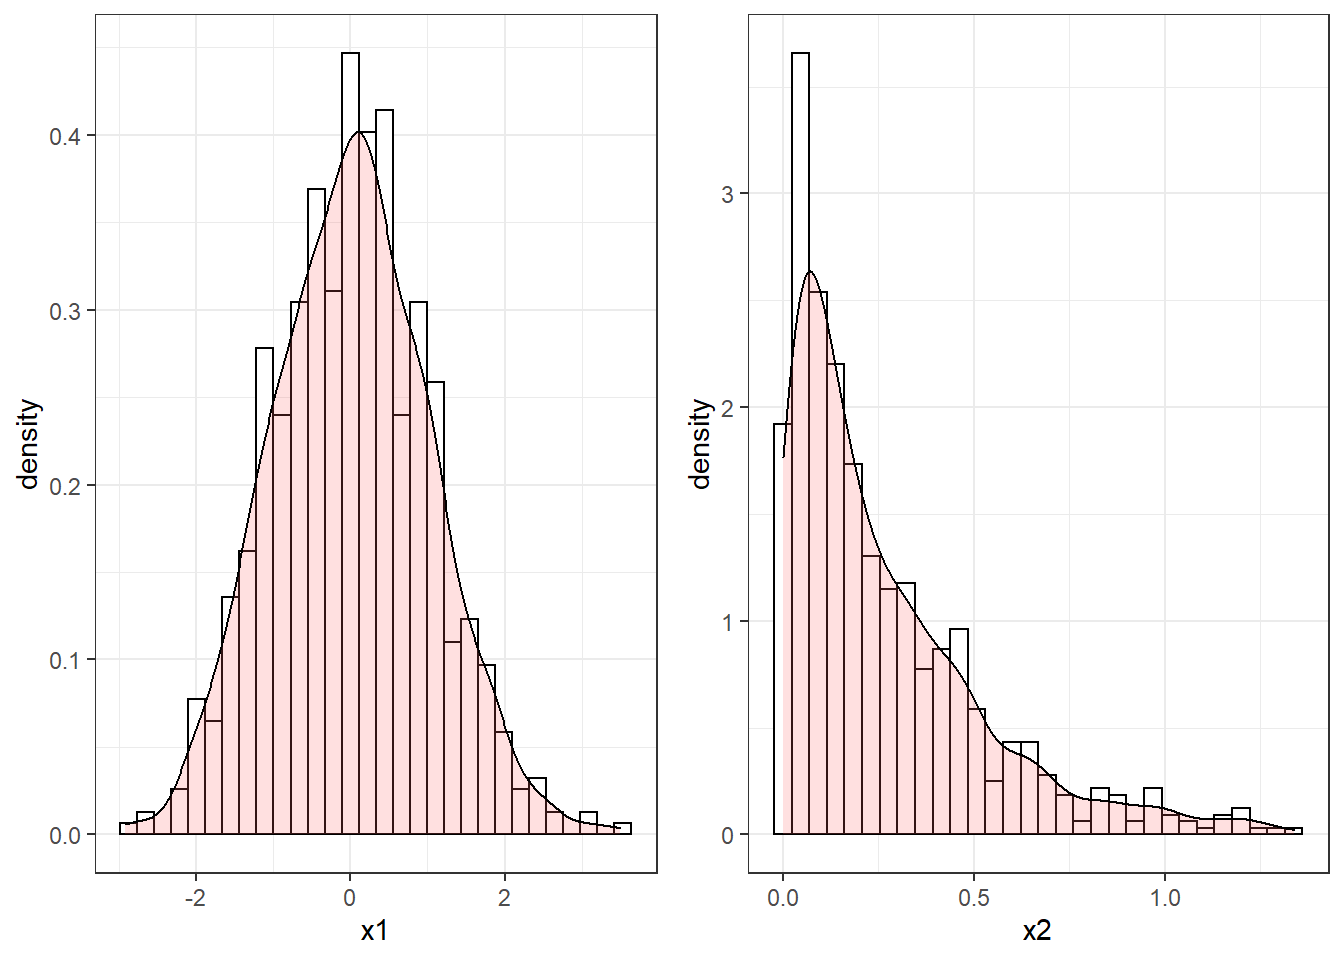
\includegraphics[width=0.5\linewidth]{SimBook_files/figure-latex/seq-1} 

}

\caption{Histograms of two sequences of randomly generated numbers}\label{fig:seq}
\end{figure}

In this chapter we will learn how to characterize randomness in a computer and how to generate numbers that appear to be random realizations of a specific random variable. We will also learn how to check if a sequence of values can be a random realization from a specific random variable.

\hypertarget{properties-of-random-numbers}{%
\section{Properties of Random Numbers}\label{properties-of-random-numbers}}

The first step to simulate numbers from a distribution is to be able to independently simulate random numbers \(u_1,u_2,\dots,u_N\) from a continuous uniform distribution between zero and one. From the previous chapter, you should remember that such a random variables has pdf
\[
f(x)=\left\{
\begin{array}{ll}
1, & 0\leq x \leq 1\\
0, &\mbox{otherwise}
\end{array}
\right.
\]
and cdf
\[
F(x)=\left\{
\begin{array}{ll}
0, & x<0\\
x, & 0\leq x \leq 1\\
1, &\mbox{otherwise}
\end{array}
\right.
\]
These two are plotted in Figure \ref{fig:uplot}.

\begin{figure}

{\centering 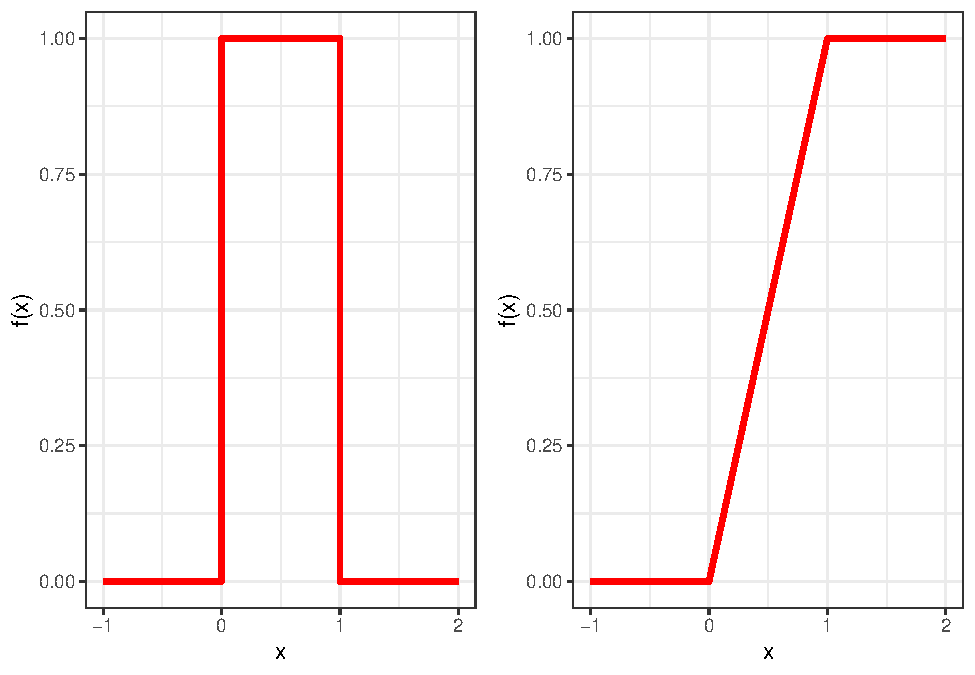
\includegraphics[width=0.5\linewidth]{SimBook_files/figure-latex/uplot-1} 

}

\caption{Pdf (left) and cdf (right) of the continuous uniform between zero and one.}\label{fig:uplot}
\end{figure}

Its expectation is 1/2 and its variance is 1/12.

This implies that if we were to divide the interval \([0,1]\) into \(n\) sub-intervals of equal length, then we would expect in each interval to have \(N/n\) observations, where \(N\) is the total number of observations.

Figure \ref{fig:uhist} shows the histograms of two sequences of numbers between zero and one: whilst the one on the left resembles the pdf of a uniform distribution, the one on the right clearly does not (it is far from being flat) and therefore it is hard to believe that such numbers follow a uniform distribution.

\begin{figure}

{\centering 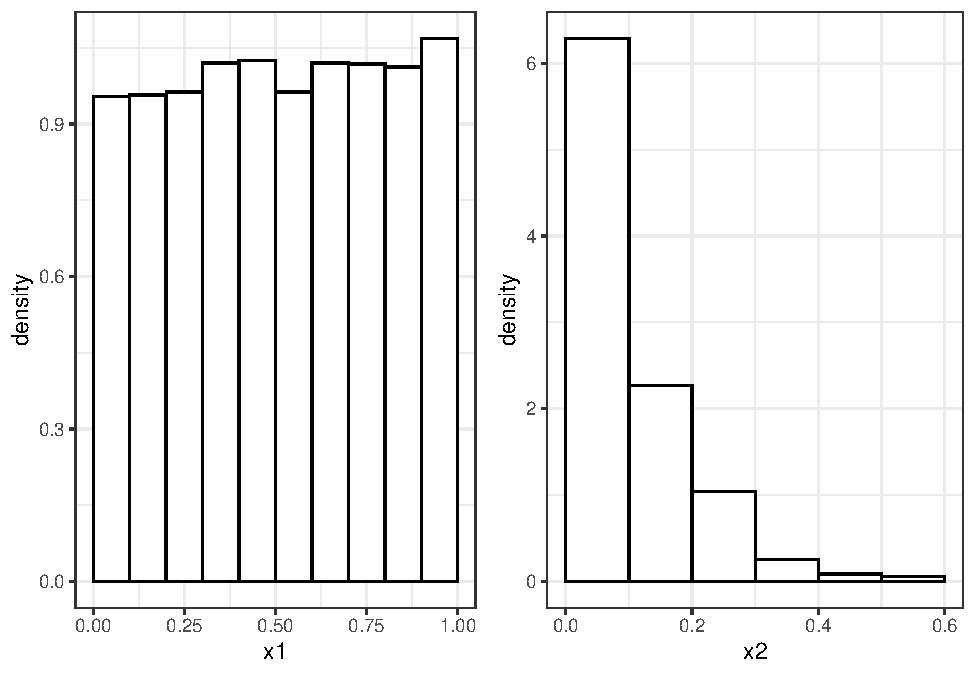
\includegraphics[width=0.5\linewidth]{SimBook_files/figure-latex/uhist-1} 

}

\caption{Histograms from two sequences of numbers between zero and one.}\label{fig:uhist}
\end{figure}

The second requirement the numbers \(u_1,\dots,u_N\) need to respect is independence. This means that the probability of observing a value in a particular sub-interval of \((0,1)\) is independent of the previous values drawn.

Consider the following sequence of numbers:
\[
\begin{array}{cccccccccc}
0.25 & 0.72 & 0.18 & 0.63 & 0.49 & 0.88 & 0.23 & 0.78 & 0.02 & 0.52
\end{array}
\]
We can notice that numbers below and above 0.5 are alternating in the sequence. We would therefore believe that after a number less than 0.5 it is much more likely to observe a number above it. This breaks the assumption of independence.

\hypertarget{pseudo-random-numbers}{%
\section{Pseudo Random Numbers}\label{pseudo-random-numbers}}

We will investigate ways to simulate numbers using algorithms in a computer. For this reason such numbers are usually called \emph{pseudo-random} numbers. Pseudo means false, in the sense that the number are not really random! They are generated according to a deterministic algorithm whose aim is to imitate as closely as possible what randomness would look like. In particular, for numbers \(u_1,\dots,u_N\) it means that they should look like independence instances of a Uniform distribution between zero and one.

Possible departures from ideal numbers are:

\begin{itemize}
\item
  the numbers are not uniformly distributed;
\item
  the mean of the numbers might not be 1/2;
\item
  the variance of the numbers might not be 1/12;
\item
  the numbers might be discrete-valued instead of continuous;
\item
  independence might not hold.
\end{itemize}

We already looked at examples of departures from the assumptions, but we will later study how to assess these departures more formally.

Before looking at how we can construct pseudo-random numbers, let's discuss some important properties/considerations that need to be taken into account when generating pseudo-random numbers:

\begin{itemize}
\item
  the random generation should be very fast. In practice, we want to use random numbers to do other computations (for example simulate a little donut shop) and such computations might be computationally intensive: if random generation were to be slow, we would not be able to perform them.
\item
  the cycle of random generated numbers should be long. The cycle is the length of the sequence before numbers start to repeat themselves.
\item
  the random numbers should be repeatable. Given a starting point of the algorithm, it should be possible to repeat the exact same sequence of numbers. This is fundamental for debugging and for reproducibility.
\item
  the method should be applicable in any programming language/platform.
\item
  and of course most importantly, the random numbers should be independent and uniformly distributed.
\end{itemize}

Repeatability of the pseudo-random numbers is worth further consideration. It is fundamental in science to be able to reproduce experiments so that the validity of results can be assessed. In R there is a specific function that allows us to do this, which is called \texttt{set.seed}. It is customary to choose as starting point of an algorithm the current year. So henceforth you will see the command:

\begin{Shaded}
\begin{Highlighting}[]
\FunctionTok{set.seed}\NormalTok{(}\DecValTok{2021}\NormalTok{)}
\end{Highlighting}
\end{Shaded}

This ensures that every time the code following \texttt{set.seed} is run, the same results will be observed. We will give below examples of this.

\hypertarget{generating-pseudo-random-numbers}{%
\section{Generating Pseudo-Random Numbers}\label{generating-pseudo-random-numbers}}

The literature on generating pseudo-random numbers is now extremely vast and it is not our purpose to review it, neither for you to learn how such algorithms work.

\hypertarget{generating-pseudo-random-numbers-in-r}{%
\subsection{Generating Pseudo-Random Numbers in R}\label{generating-pseudo-random-numbers-in-r}}

R has all the capabilities to generate such numbers. This can be done with the function \texttt{runif}, which takes one input: the number of observations to generate. So for instance:

\begin{Shaded}
\begin{Highlighting}[]
\FunctionTok{set.seed}\NormalTok{(}\DecValTok{2021}\NormalTok{)}
\FunctionTok{runif}\NormalTok{(}\DecValTok{10}\NormalTok{)}
\end{Highlighting}
\end{Shaded}

\begin{verbatim}
##  [1] 0.4512674 0.7837798 0.7096822 0.3817443 0.6363238 0.7013460 0.6404389
##  [8] 0.2666797 0.8154215 0.9829869
\end{verbatim}

generates ten random numbers between zero and one. Notice that if we repeat the same code we get the same result since we fixed the so-called \emph{seed} of the simulation.

\begin{Shaded}
\begin{Highlighting}[]
\FunctionTok{set.seed}\NormalTok{(}\DecValTok{2021}\NormalTok{)}
\FunctionTok{runif}\NormalTok{(}\DecValTok{10}\NormalTok{)}
\end{Highlighting}
\end{Shaded}

\begin{verbatim}
##  [1] 0.4512674 0.7837798 0.7096822 0.3817443 0.6363238 0.7013460 0.6404389
##  [8] 0.2666797 0.8154215 0.9829869
\end{verbatim}

Conversely, if we were to simply run the code \texttt{runif(10)} we would get a different result.

\begin{Shaded}
\begin{Highlighting}[]
\FunctionTok{runif}\NormalTok{(}\DecValTok{10}\NormalTok{)}
\end{Highlighting}
\end{Shaded}

\begin{verbatim}
##  [1] 0.02726706 0.83749040 0.60324073 0.56745337 0.82005281 0.25157128
##  [7] 0.50549403 0.86753810 0.95818157 0.54569770
\end{verbatim}

\hypertarget{linear-congruential-method}{%
\subsection{Linear Congruential Method}\label{linear-congruential-method}}

Although we will use the functions already implemented in R, it is useful to at least introduce one of the most classical algorithms to simulate random numbers, called the \emph{linear congruential method}.
This produces a sequence of integers \(x_1,x_2,x_3\) between 0 and \(m-1\) using the recursion:
\[
x_{i}=(ax_{i-1}+c)\mod m, \hspace{1cm} \mbox{for } i = 1,2,\dots
\]
Some comments:

\begin{itemize}
\item
  \(\mod m\) is the remainder of the integer division by \(m\). For instance \(5 \mod 2\) is one and \(4\mod 2\) is zero.
\item
  therefore, the algorithm generates integers between 0 and \(m-1\).
\item
  there are three parameters that need to be chosen \(a, c\) and \(m\).
\item
  the value \(x_0\) is the \emph{seed} of the algorithm.
\end{itemize}

Random numbers between zero and one can be derived by setting
\[
u_i= x_i/m.
\]

It can be shown that the method works well for specific choices of \(a\), \(c\) and \(m\), which we will not discuss here.

Let's look at an implementation.

\begin{Shaded}
\begin{Highlighting}[]
\NormalTok{lcm }\OtherTok{\textless{}{-}} \ControlFlowTok{function}\NormalTok{(N, x0, a, c, m)\{}
\NormalTok{   x }\OtherTok{\textless{}{-}} \FunctionTok{rep}\NormalTok{(}\DecValTok{0}\NormalTok{,N)}
\NormalTok{   x[}\DecValTok{1}\NormalTok{] }\OtherTok{\textless{}{-}}\NormalTok{ x0}
   \ControlFlowTok{for}\NormalTok{ (i }\ControlFlowTok{in} \DecValTok{2}\SpecialCharTok{:}\NormalTok{N) x[i] }\OtherTok{\textless{}{-}}\NormalTok{ (a}\SpecialCharTok{*}\NormalTok{x[i}\DecValTok{{-}1}\NormalTok{]}\SpecialCharTok{+}\NormalTok{c)}\SpecialCharTok{\%\%}\NormalTok{m}
\NormalTok{   u }\OtherTok{\textless{}{-}}\NormalTok{ x}\SpecialCharTok{/}\NormalTok{m}
   \FunctionTok{return}\NormalTok{(u)}
\NormalTok{\}}
\end{Highlighting}
\end{Shaded}

\begin{Shaded}
\begin{Highlighting}[]
\FunctionTok{lcm}\NormalTok{(}\AttributeTok{N =} \DecValTok{8}\NormalTok{, }\AttributeTok{x0 =} \DecValTok{4}\NormalTok{, }\AttributeTok{a =} \DecValTok{13}\NormalTok{, }\AttributeTok{c =} \DecValTok{0}\NormalTok{, }\AttributeTok{m =} \DecValTok{64}\NormalTok{)}
\end{Highlighting}
\end{Shaded}

\begin{verbatim}
## [1] 0.0625 0.8125 0.5625 0.3125 0.0625 0.8125 0.5625 0.3125
\end{verbatim}

We can see that this specific choice of parameters is quite bad: it has cycle 4! After 4 numbers the sequence repeats itself and we surely would not like to use this in practice.

In general you should not worry of these issues, R does things properly for you!

\hypertarget{testing-randomness}{%
\section{Testing Randomness}\label{testing-randomness}}

Now we turn to the following question: given a sequence of numbers \(u_1,\dots,u_N\) how can we test if they are independent realizations of a Uniform random variable between zero and one?

We therefore need to check if the distribution of the numbers is uniform and if they are actually independent.

\hypertarget{testing-uniformity}{%
\subsection{Testing Uniformity}\label{testing-uniformity}}

A simple first method to check if the numbers are uniform is to create an histogram of the data and to see if the histogram is reasonably flat. We already saw how to assess this, but let's check if \texttt{runif} works well. Simple histograms can be created in \texttt{R} using \texttt{hist} (or if you want you can use \texttt{ggplot}).

\begin{Shaded}
\begin{Highlighting}[]
\FunctionTok{set.seed}\NormalTok{(}\DecValTok{2021}\NormalTok{)}
\NormalTok{u }\OtherTok{\textless{}{-}} \FunctionTok{runif}\NormalTok{(}\DecValTok{5000}\NormalTok{)}
\FunctionTok{hist}\NormalTok{(u)}
\end{Highlighting}
\end{Shaded}

\begin{figure}

{\centering 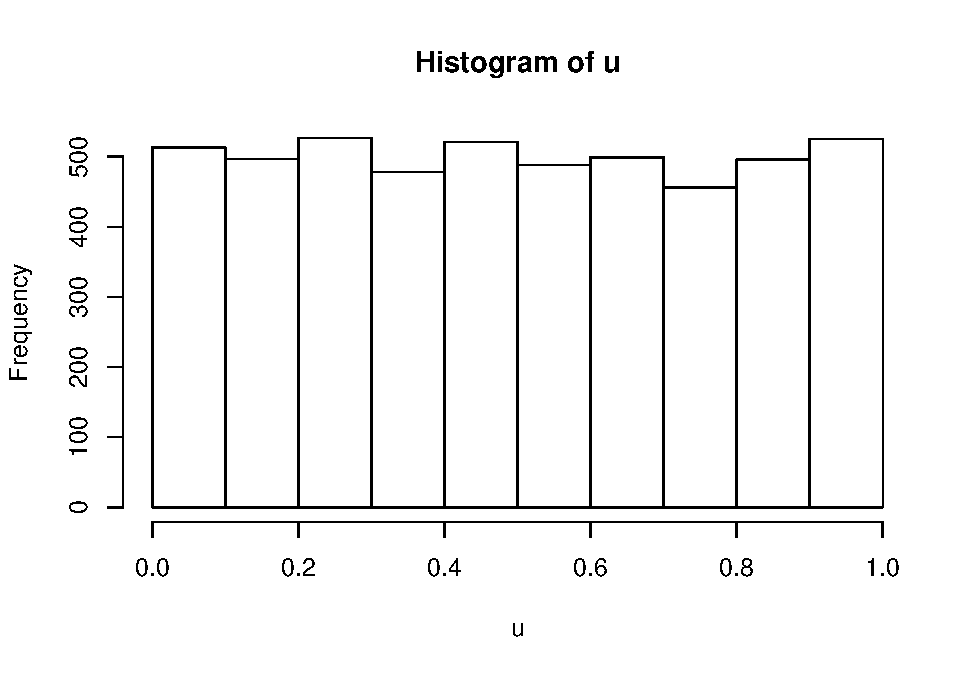
\includegraphics[width=0.5\linewidth]{SimBook_files/figure-latex/hist-1} 

}

\caption{Histogram of a sequence of uniform numbers}\label{fig:hist}
\end{figure}

We can see that the histogram is reasonably flat and therefore the assumption of uniformity seems to hold.

Although the histogram is quite informative, it is not a fairly formal method. We could on the other hand look at tests of hypotheses of this form:
\begin{align*}
H_0: & \;\;u_i \mbox{ is uniform between zero and one, } i=1,2,\dots\\
H_a: & \;\;u_i \mbox{ is not uniform between zero and one, } i=1,2,\dots\\
\end{align*}

The null hypothesis is thus that the numbers are indeed uniform, whilst the alternative states that the numbers are not. If we reject the null hypothesis, which happens if the p-value of the test is very small (or smaller than a critical value \(\alpha\) of our choice), then we would believe that the sequence of numbers is not uniform.

There are various ways to carry out such a test, but we will consider here only one: the so-called \emph{Kolmogorov-Smirnov Test}. We will not give all details of this test, but only its interpretation and implementation.

In order to understand how the test works we need to briefly introduce the concept of \emph{empirical cumulative distribution function} or \emph{ecdf}. The ecdf \(\hat{F}\) is the cumulative distribution function computed from a sequence of \(N\) numbers as
\[
\hat{F}(t)= \frac{\mbox{numbers in the sequence }\leq t}{N}
\]

Let's consider the following example.

\begin{Shaded}
\begin{Highlighting}[]
\NormalTok{data }\OtherTok{\textless{}{-}} \FunctionTok{data.frame}\NormalTok{(}\AttributeTok{u=} \FunctionTok{c}\NormalTok{(}\FloatTok{0.1}\NormalTok{,}\FloatTok{0.2}\NormalTok{,}\FloatTok{0.4}\NormalTok{,}\FloatTok{0.8}\NormalTok{,}\FloatTok{0.9}\NormalTok{))}
\FunctionTok{ggplot}\NormalTok{(data,}\FunctionTok{aes}\NormalTok{(u)) }\SpecialCharTok{+} \FunctionTok{stat\_ecdf}\NormalTok{(}\AttributeTok{geom =} \StringTok{"step"}\NormalTok{) }\SpecialCharTok{+} \FunctionTok{theme\_bw}\NormalTok{() }\SpecialCharTok{+} \FunctionTok{ylab}\NormalTok{(}\StringTok{"ECDF"}\NormalTok{)}
\end{Highlighting}
\end{Shaded}

\begin{figure}

{\centering 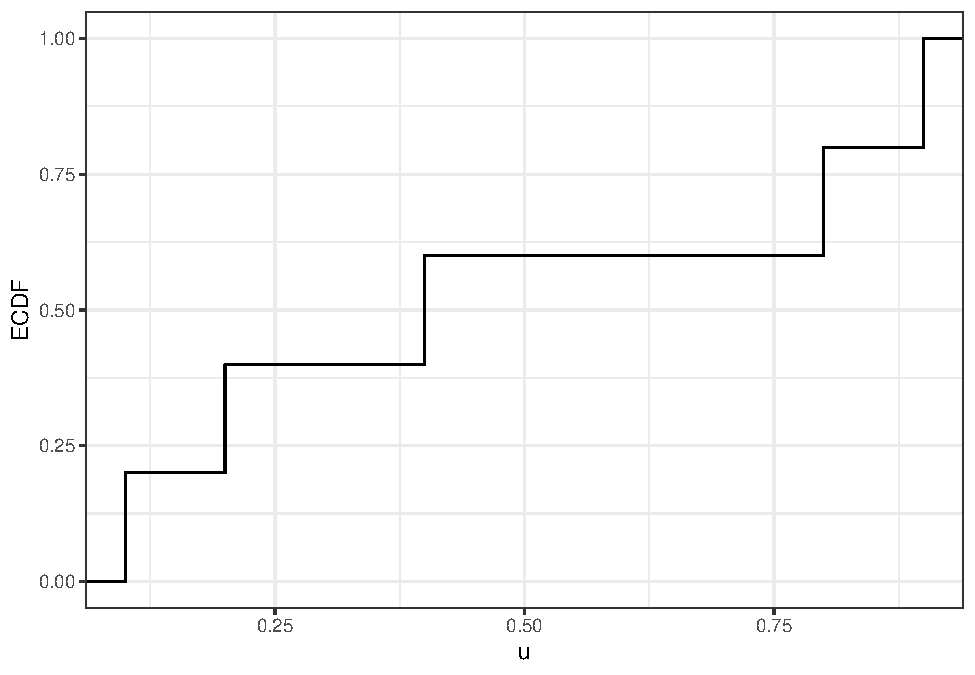
\includegraphics[width=0.5\linewidth]{SimBook_files/figure-latex/ecdf-1} 

}

\caption{Ecdf of a simple sequence of numbers}\label{fig:ecdf}
\end{figure}

For instance, since there are 3 numbers out of 5 in the vector \texttt{u} that are less than 0.7, then \(\hat{F}(0.7)=3/5\).

The idea behind the Kolmogorov-Smirnov test is to quantify how similar the ecdf computed from a sequence of data is to the one of the uniform distribution which is represented by a straight line (see Figure \ref{fig:uplot}).

As an example consider Figure \ref{fig:Kol}. The step functions are computed from two different sequences of numbers between one and zero, whilst the straight line is the cdf of the uniform distribution. By looking at the plots, we would more strongly believe that the sequence in the left plot is uniformly distributed, since the step function is much more closer to the theoretical straight line.

\begin{figure}

{\centering 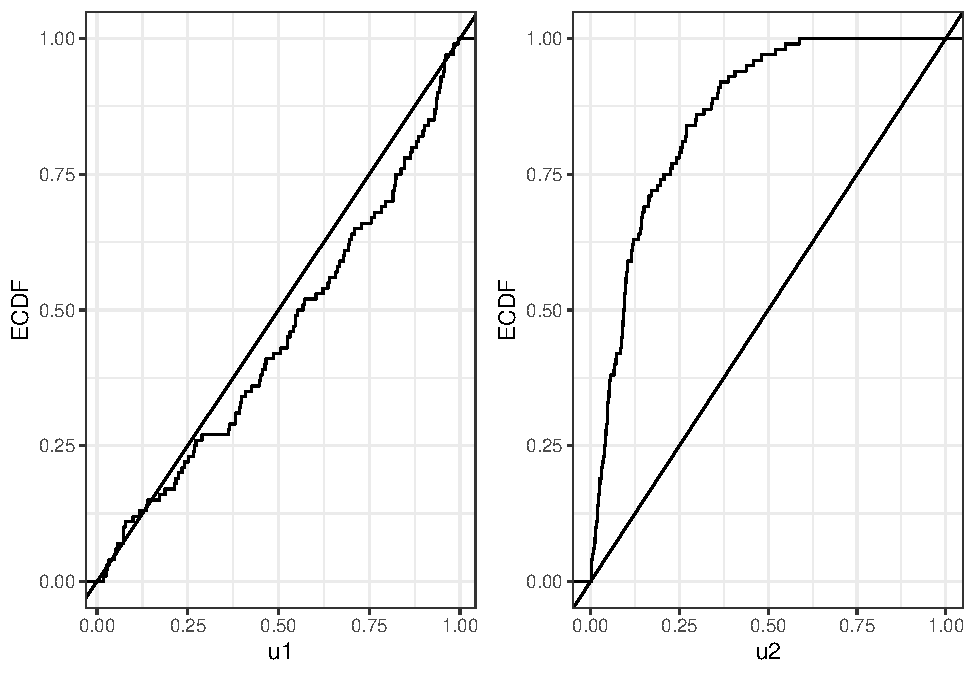
\includegraphics{SimBook_files/figure-latex/Kol-1} 

}

\caption{Comparison between ecdf and cdf of the uniform for two sequences of numbers}\label{fig:Kol}
\end{figure}

The Kolmogorov-Smirnov test formally embeds this idea of similarity between the ecdf and the cdf of the uniform in a test of hypothesis. The function \texttt{ks.test} implements this test in R. For the two sequences in Figure @ref\{fig:Kol\} \texttt{u1} (left plot) and \texttt{u2} (right plot), the test can be implemented as following:

\begin{Shaded}
\begin{Highlighting}[]
\FunctionTok{ks.test}\NormalTok{(u1,}\StringTok{"punif"}\NormalTok{)}
\end{Highlighting}
\end{Shaded}

\begin{verbatim}
## 
##  One-sample Kolmogorov-Smirnov test
## 
## data:  u1
## D = 0.11499, p-value = 0.142
## alternative hypothesis: two-sided
\end{verbatim}

\begin{Shaded}
\begin{Highlighting}[]
\FunctionTok{ks.test}\NormalTok{(u2,}\StringTok{"punif"}\NormalTok{)}
\end{Highlighting}
\end{Shaded}

\begin{verbatim}
## 
##  One-sample Kolmogorov-Smirnov test
## 
## data:  u2
## D = 0.56939, p-value < 2.2e-16
## alternative hypothesis: two-sided
\end{verbatim}

From the results that the p-value of the test for the sequence \texttt{u1} is 0.142 and so we would not reject the null hypothesis that the sequence is uniformly distributed. On the other hand the p-value for the test over the sequence \texttt{u2} has an extremely small p-value therefore suggesting that we reject the null hypothesis and conclude that the sequence is not uniformly distributed. This confirms our intuition by looking at the plots in Figure \ref{fig:Kol}.

\hypertarget{testing-independence}{%
\subsection{Testing Independence}\label{testing-independence}}

The second requirement that a sequence of pseudo-random numbers must have is independence. We already saw an example of when this might happen: a high number was followed by a low number and vice versa.

We will consider tests of the form:

\begin{align*}
H_0: & \;\;u_1,\dots,u_N \mbox{ are independent }\\
H_a: & \;\;u_1,\dots,u_N \mbox{ are not independent }
\end{align*}

So the null hypothesis is that the sequence is of independent numbers against the alternative that they are not. If the p-value of such a test is small we would then reject the null-hypothesis of independence.

In order to devise such a test, we need to come up with a way to quantify how dependent numbers in a sequence are with each other. Again, there are many ways one could do this, but we consider here only one.

You should already be familiar with the idea of \emph{correlation}: this tells you how to variables are linearly dependent of each other. There is a similar idea which extends in a way correlation to the case when it is computed between a sequence of numbers and itself, which is called \emph{autocorrelation}. We will not give the details about this, but just the interpretation (you will learn a lot more about this in Time Series).

Let's briefly recall the idea behind correlation. Suppose you have two sequences of numbers \(u_1,\dots,u_N\) and \(w_1,\dots,w_N\). To compute the correlation you would look at the pairs \((u_1,w_1),(u_2,w_2),\dots, (u_N,w_N)\) and assess how related the numbers within a pair \((u_i,w_i)\) are. Correlation, which is a number between -1 and 1, assesses how related the sequences are: the closer the number is to one in absolute value, the stronger the relationship.

Now however we have just one sequence of numbers \(u_1,\dots,u_N\). So for instance we could look at pairs \((u_1,u_2), (u_2,u_3), \dots, (u_{N-1},u_{N})\) which consider two consecutive numbers and compute their correlation. Similarly we could compute the correlation between \((u_1,u_{1+k}), (u_2,u_{2+k}),\dots, (u_{N-k},u_N)\) between each number in the sequence and the one k-positions ahead. This is what we call \emph{autocorrelation of lag k}.

If autocorrelations of various lags are close to zero, this gives an indication that the data is independent. If on the other hand, the autocorrelation at some lags is large, then there is an indication of dependence in the sequence of random numbers. Autocorrelations are computed and plotted in \texttt{R} using \texttt{acf} and reported in Figure \ref{fig:acf}.

\begin{Shaded}
\begin{Highlighting}[]
\FunctionTok{set.seed}\NormalTok{(}\DecValTok{2021}\NormalTok{)}
\NormalTok{u1 }\OtherTok{\textless{}{-}} \FunctionTok{runif}\NormalTok{(}\DecValTok{200}\NormalTok{)}
\FunctionTok{acf}\NormalTok{(u1)}
\end{Highlighting}
\end{Shaded}

\begin{figure}

{\centering 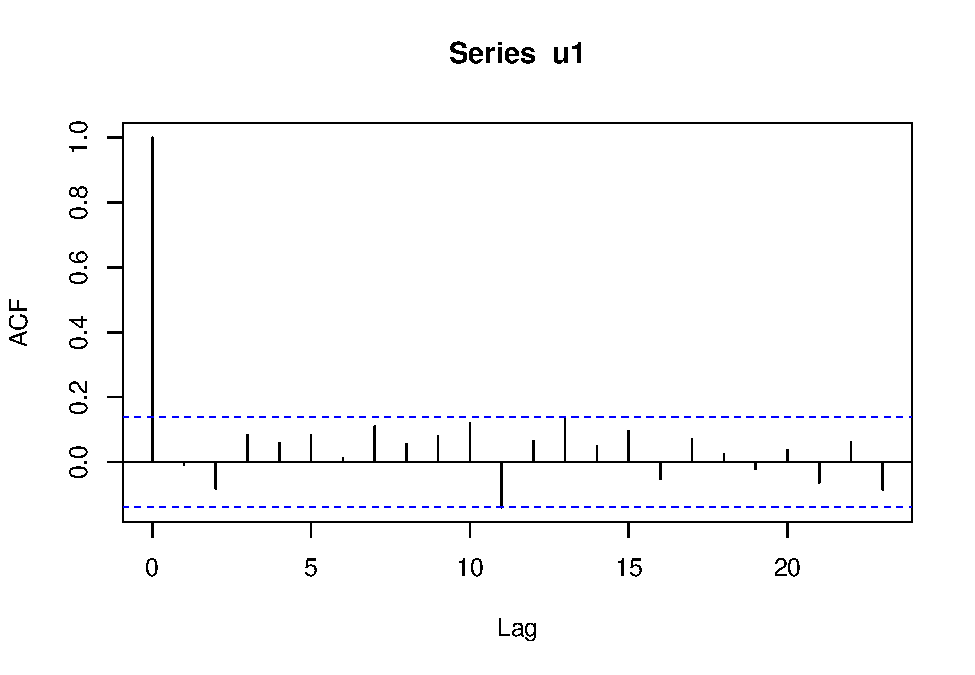
\includegraphics[width=0.5\linewidth]{SimBook_files/figure-latex/acf-1} 

}

\caption{Autocorrelations for a sequence of random uniform numbers}\label{fig:acf}
\end{figure}

The bars in Figure \ref{fig:acf} are the autocorrelations at various lags, whilst the dashed blue lines are confidence bands: if a bar is within the bands it means that we cannot reject the hypothesis that the autocorrelation of the associated lag is equal to zero. Notice that the first bar is lag 0: it computes the correlation for the sample \((u_1,u_1),(u_2,u_2),\dots,(u_N,u_N)\) and therefore it is always equal to one. You should never worry about this bar. Since all the bars are within the confidence bands, we believe that all autocorrelations are not different from zero and consequently that the data is independent (it was indeed generated using `runif``).

Figure \ref{fig:acf2} reports the autocorrelations of a sequence of numbers which is not independent. Although the histogram shows that the data is uniformly distributed, we would not believe that the sequence is of independent numbers since autocorrelations are very large and outside the bands.

\begin{Shaded}
\begin{Highlighting}[]
\NormalTok{u2 }\OtherTok{\textless{}{-}} \FunctionTok{rep}\NormalTok{(}\DecValTok{1}\SpecialCharTok{:}\DecValTok{10}\NormalTok{,}\AttributeTok{each =} \DecValTok{4}\NormalTok{,}\AttributeTok{times =} \DecValTok{10}\NormalTok{)}\SpecialCharTok{/}\DecValTok{10} \SpecialCharTok{+} \FunctionTok{rnorm}\NormalTok{(}\DecValTok{400}\NormalTok{,}\DecValTok{0}\NormalTok{,}\FloatTok{0.02}\NormalTok{) }
\NormalTok{u2 }\OtherTok{\textless{}{-}}\NormalTok{ (u2 }\SpecialCharTok{{-}} \FunctionTok{min}\NormalTok{(u2))}\SpecialCharTok{/}\NormalTok{(}\FunctionTok{max}\NormalTok{(u2)}\SpecialCharTok{{-}}\FunctionTok{min}\NormalTok{(u2))}
\FunctionTok{par}\NormalTok{(}\AttributeTok{mfrow=}\FunctionTok{c}\NormalTok{(}\DecValTok{1}\NormalTok{,}\DecValTok{2}\NormalTok{))}
\FunctionTok{hist}\NormalTok{(u2)}
\FunctionTok{acf}\NormalTok{(u2)}
\end{Highlighting}
\end{Shaded}

\begin{figure}

{\centering 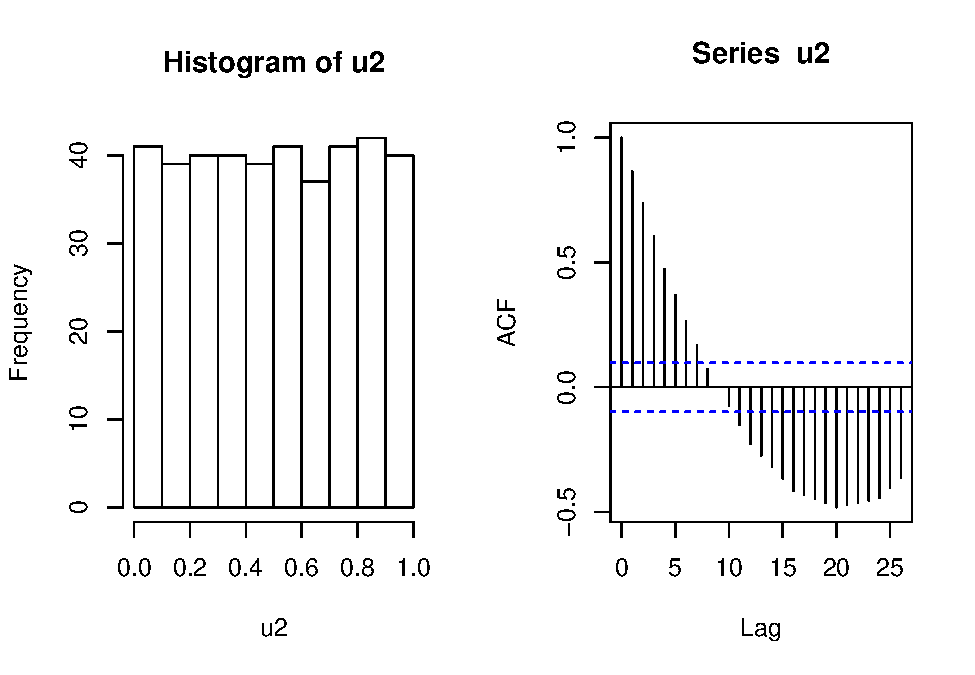
\includegraphics{SimBook_files/figure-latex/acf2-1} 

}

\caption{Histogram and autocorrelations of a sequence of uniform numbers which are not independent}\label{fig:acf2}
\end{figure}

A test of hypothesis for independence can be created by checking if any of the autocorrelations up to a specific lag are different from zero. This is implemented in the function \texttt{Box.test} in R. The first input is the sequence of numbers to consider, the second is the largest lag we want to consider. Let's compute it for the two sequences \texttt{u1} and \texttt{u2} above.

\begin{Shaded}
\begin{Highlighting}[]
\FunctionTok{Box.test}\NormalTok{(u1, }\AttributeTok{lag =} \DecValTok{5}\NormalTok{)}
\end{Highlighting}
\end{Shaded}

\begin{verbatim}
## 
##  Box-Pierce test
## 
## data:  u1
## X-squared = 4.8518, df = 5, p-value = 0.4342
\end{verbatim}

\begin{Shaded}
\begin{Highlighting}[]
\FunctionTok{Box.test}\NormalTok{(u2, }\AttributeTok{lag =} \DecValTok{5}\NormalTok{)}
\end{Highlighting}
\end{Shaded}

\begin{verbatim}
## 
##  Box-Pierce test
## 
## data:  u2
## X-squared = 807.1, df = 5, p-value < 2.2e-16
\end{verbatim}

Here we chose a lag up to 5 (it is usually not useful to consider larger lags). The test confirms our observations of the autocorrelations. For the sequence \texttt{u1} generated with \texttt{runif} the test has a high p-value and therefore we cannot reject the hypothesis of independence. For the second sequence \texttt{u2} which had very large autocorrelations the p-value is very small and therefore we reject the hypothesis of independence.

\hypertarget{random-variate-generation}{%
\section{Random Variate Generation}\label{random-variate-generation}}

Up to this point we have investigated how to generate numbers between 0 and 1 and how to assess the quality of those randomly generated numbers.

For simulation models we want to be more generally able to simulate observations that appear to be realizations of random variables with known distributions. We now study how this can be done. But before this, let's see how R implements random variate generation.

\hypertarget{random-generation-in-r}{%
\subsection{Random Generation in R}\label{random-generation-in-r}}

In the next few sections we will learn results that allow for the simulation of random observations from generic distributions. No matter how the methods work, they have a very simple and straightforward implementation in R.

We have already learned that we can simulate observations from the uniform between zero and one using the code \texttt{runif(N)} where \texttt{N} is the number of observations to simulate. We can notice that it is similar to the commands \texttt{dunif} and \texttt{punif} we have already seen for the pdf and cdf of the uniform.

Not surprisingly we can generate observations from any random variable using the syntax \texttt{r} followed by the naming of the variable chosen. So for instance:

\begin{itemize}
\item
  \texttt{runif} generates random observations from the Uniform;
\item
  \texttt{rnorm} generates random observations from the Normal;
\item
  \texttt{rexp} generates random observations from the Exponential;
\item
  \texttt{rbinom} generates random observations from the Binomial;
\item
  \texttt{rpois} generates random observations from the Poisson;
\end{itemize}

Each of these functions takes as first input the number of observations that we want to simulate. They then have additional inputs that can be given, which depend on the random variable chosen and are the same that we saw in the past.

So for instance

\begin{Shaded}
\begin{Highlighting}[]
\FunctionTok{rnorm}\NormalTok{(}\DecValTok{10}\NormalTok{, }\AttributeTok{mean =} \DecValTok{1}\NormalTok{, }\AttributeTok{sd =} \DecValTok{2}\NormalTok{)}
\end{Highlighting}
\end{Shaded}

generates ten observations from a Normal distribution with mean 1 and standard deviation 2.

\hypertarget{the-inverse-transform-method}{%
\subsection{The Inverse Transform Method}\label{the-inverse-transform-method}}

The simplest method to simulate observations from generic random variables is the so-called \emph{inverse transform method}.

Suppose we are interested in a random variable \(X\) whose cdf is \(F\). We must assume that \(F\) is:

\begin{itemize}
\item
  known and written in closed-form;
\item
  continuous;
\item
  strictly increasing.
\end{itemize}

Then one can prove that
\[
X = F^{-1}(U),
\]
where \(F^{-1}\) is the inverse of \(F\) and \(U\) is a continuous uniform distribution between zero and one.

The above results gives us the following algorithm to simulate observations from a random variable \(X\) with distribution \(F\):

\begin{enumerate}
\def\labelenumi{\arabic{enumi}.}
\item
  compute the inverse \(F^{-1}\) of \(F\);
\item
  generate independent random observations \(u_1,u_2,\dots,u_N\) from a Uniform between zero and one;
\item
  compute \(x_1=F^{-1}(u_1), x_2=F^{-1}(u_2),\dots,x_N=F^{-1}(u_n)\).
\end{enumerate}

Then \(x_1,x_2,\dots,x_N\) are independent random observations of the random variable \(X\).

So the above algorithm can be applied to generate observations from continuous random variables with a cdf in closed-form. Therefore, for instance the above algorithm cannot be straightforwardly used for Normals. However it can be used to simulate Exponential and Uniform distributions. Furthermore, it cannot be directly used to simulate discrete random variables. A simple adaptation of this method, which we will not see here, can however be used for discrete random variables.

\hypertarget{simulating-exponentials}{%
\subsubsection{Simulating Exponentials}\label{simulating-exponentials}}

Recall that if \(X\) is Exponential with parameter \(\lambda\) then its cdf is
\[
F(x)= 1- e^{-\lambda x}, \hspace{1cm} \mbox{for } x\geq 0
\]
Suppose we want to simulate observations \(x_1,\dots,x_N\) from such a distribution.

\begin{enumerate}
\def\labelenumi{\arabic{enumi}.}
\item
  First we need to compute the inverse of \(F\). This means solving the equation:
  \[
  1-e^{-\lambda x} = u
  \]
  for \(x\). This can be done following the steps:
  \begin{eqnarray*}
  1-e^{-\lambda x} &=& u\\
  e^{-\lambda x} &=& 1 - u\\
  -\lambda x &=& \log(1-u)\\
  x &=& -\frac{1}{\lambda}\log(1-u)
  \end{eqnarray*}
  So \(F^{-1}(u)=-\log(1-u)/\lambda\).
\item
  Second we need to simulate random uniform observations using \texttt{runif}.
\item
  Last, we apply the inverse function to the randomly simulated observations.
\end{enumerate}

Let's give the R code.

\begin{Shaded}
\begin{Highlighting}[]
\FunctionTok{set.seed}\NormalTok{(}\DecValTok{2021}\NormalTok{)}
\CommentTok{\# Define inverse function}
\NormalTok{invF }\OtherTok{\textless{}{-}} \ControlFlowTok{function}\NormalTok{(u,lambda) }\SpecialCharTok{{-}}\FunctionTok{log}\NormalTok{(}\DecValTok{1}\SpecialCharTok{{-}}\NormalTok{u)}\SpecialCharTok{/}\NormalTok{lambda}
\CommentTok{\# Simulate 5 uniform observations}
\NormalTok{u }\OtherTok{\textless{}{-}} \FunctionTok{runif}\NormalTok{(}\DecValTok{5}\NormalTok{)}
\CommentTok{\# Compute the inverse }
\FunctionTok{invF}\NormalTok{(u, }\AttributeTok{lambda =} \DecValTok{2}\NormalTok{)}
\end{Highlighting}
\end{Shaded}

\begin{verbatim}
## [1] 0.3000720 0.7657289 0.6183896 0.2404265 0.5057456
\end{verbatim}

First we defined the inverse function of an Exponential with parameter \texttt{lambda} in \texttt{invF}. Then we simulated five observations from a uniform. Last we applied the function \texttt{invF} for a parameter \texttt{lambda} equal to two. The output are therefore five observations from an Exponential random variable with parameter 2.

\hypertarget{simulating-generic-uniforms}{%
\subsubsection{Simulating Generic Uniforms}\label{simulating-generic-uniforms}}

We know how to simulate uniformly between 0 and 1, but we do not know how to simulate uniformly between two generic values \(a\) and \(b\).

Recall that the cdf of the uniform distribution between \(a\) and \(b\) is
\[
F(x)=\frac{x-a}{b-a}, \hspace{2cm} \mbox{for } a\leq x \leq b
\]
The inverse transform method requires the inverse of \(F\), which using simple algebra can be computed as
\[
F^{-1}(u)=a + (b-a)u
\]
So given a sequence \(u_1,\dots,u_N\) of random observations from a Uniform between 0 and 1, we can simulate numbers at uniform between \(a\) and \(b\) by computing
\[
x_1 = a + (b-a)u_1,\dots, x_N=a+(b-a)u_N
\]
In R:

\begin{Shaded}
\begin{Highlighting}[]
\FunctionTok{set.seed}\NormalTok{(}\DecValTok{2021}\NormalTok{)}
\NormalTok{a }\OtherTok{\textless{}{-}} \DecValTok{2}
\NormalTok{b }\OtherTok{\textless{}{-}} \DecValTok{6}
\NormalTok{a }\SpecialCharTok{+}\NormalTok{ (b}\SpecialCharTok{{-}}\NormalTok{a)}\SpecialCharTok{*}\FunctionTok{runif}\NormalTok{(}\DecValTok{5}\NormalTok{)}
\end{Highlighting}
\end{Shaded}

\begin{verbatim}
## [1] 3.805069 5.135119 4.838729 3.526977 4.545295
\end{verbatim}

The code simulates five observations from a Uniform between two and six. This can be equally achieved by simply using:

\begin{Shaded}
\begin{Highlighting}[]
\FunctionTok{set.seed}\NormalTok{(}\DecValTok{2021}\NormalTok{)}
\FunctionTok{runif}\NormalTok{(}\DecValTok{5}\NormalTok{, }\AttributeTok{min =} \DecValTok{2}\NormalTok{, }\AttributeTok{max =} \DecValTok{6}\NormalTok{)}
\end{Highlighting}
\end{Shaded}

\begin{verbatim}
## [1] 3.805069 5.135119 4.838729 3.526977 4.545295
\end{verbatim}

Notice that since we fixed the seed, the two methods return exactly the same sequence of numbers.

\hypertarget{simulating-bernoulli-and-binomial}{%
\subsection{Simulating Bernoulli and Binomial}\label{simulating-bernoulli-and-binomial}}

Bernoulli random variables represent binary experiments with a probability of success equal to \(\theta\). A simple simulation algorithm to simulate one Bernoulli observation is:

\begin{enumerate}
\def\labelenumi{\arabic{enumi}.}
\item
  generate \(u\) uniformly between zero and one;
\item
  if \(u< \theta\) set \(x=0\), otherwise \(x=1\).
\end{enumerate}

We will not prove that this actually works, but it intuitively does. Let's code it in R.

\begin{Shaded}
\begin{Highlighting}[]
\FunctionTok{set.seed}\NormalTok{(}\DecValTok{2021}\NormalTok{)}
\NormalTok{theta }\OtherTok{\textless{}{-}} \FloatTok{0.5}
\NormalTok{u }\OtherTok{\textless{}{-}} \FunctionTok{runif}\NormalTok{(}\DecValTok{5}\NormalTok{)}
\NormalTok{x }\OtherTok{\textless{}{-}} \FunctionTok{ifelse}\NormalTok{(u }\SpecialCharTok{\textless{}}\NormalTok{ theta, }\DecValTok{0}\NormalTok{, }\DecValTok{1}\NormalTok{)}
\NormalTok{x}
\end{Highlighting}
\end{Shaded}

\begin{verbatim}
## [1] 0 1 1 0 1
\end{verbatim}

So here we simulated five observations from a Bernoulli with parameter 0.5: the toss of a fair coin. Three times the coin showed head, and twice tails.

From this comment, it is easy to see how to simulate one observation from a Binomial: by simply summing the randomly generated observations from Bernoullis. So if we were to sum the five numbers above, we would get one random observations from a Binomial with parameter \(n=5\) and \(\theta=0.5\).

\hypertarget{simulating-other-distributions}{%
\subsection{Simulating Other Distributions}\label{simulating-other-distributions}}

There are many other algorithms that allow to simulate specific as well as generic random variables. Since these are a bit more technical we will not consider them here, but it is important for you to know that we now can simulate basically any random variable you are interested in!

\hypertarget{testing-generic-simulation-sequences}{%
\section{Testing Generic Simulation Sequences}\label{testing-generic-simulation-sequences}}

In previous sections we spent a lot of effort in assesing if a sequence of numbers could have been a random sequence of independent numbers from a Uniform distribution between zero and one.

Now we will look at the same question, but considering generic distributions we might be interested in. Recall that we had to check two aspects:

\begin{enumerate}
\def\labelenumi{\arabic{enumi}.}
\item
  if the random sequence had the same distribution as the theoretical one (in previous sections Uniform between zero and one);
\item
  if the sequence was of independent numbers
\end{enumerate}

We will see that the tools to perform these steps are basically the same.

\hypertarget{testing-distribution-fit}{%
\subsection{Testing Distribution Fit}\label{testing-distribution-fit}}

There are various ways to check if the random sequence of observations has the same distribution as the theoretical one.

\hypertarget{histogram}{%
\subsubsection{Histogram}\label{histogram}}

First, we could construct an histogram of the data sequence and compare it to the theoretical distribution. Suppose we have a sequence of numbers \texttt{x1} that we want to assess if it simulated from a Standard Normal distribution.

\begin{Shaded}
\begin{Highlighting}[]
\FunctionTok{ggplot}\NormalTok{(x1, }\FunctionTok{aes}\NormalTok{(x1)) }\SpecialCharTok{+}
   \FunctionTok{geom\_line}\NormalTok{(}\FunctionTok{aes}\NormalTok{(}\AttributeTok{y =}\NormalTok{ ..density.., }\AttributeTok{colour =} \StringTok{\textquotesingle{}Empirical\textquotesingle{}}\NormalTok{), }\AttributeTok{stat =} \StringTok{\textquotesingle{}density\textquotesingle{}}\NormalTok{) }\SpecialCharTok{+}
   \FunctionTok{stat\_function}\NormalTok{(}\AttributeTok{fun =}\NormalTok{ dnorm, }\FunctionTok{aes}\NormalTok{(}\AttributeTok{colour =} \StringTok{\textquotesingle{}Normal\textquotesingle{}}\NormalTok{)) }\SpecialCharTok{+}      
   \FunctionTok{geom\_histogram}\NormalTok{(}\FunctionTok{aes}\NormalTok{(}\AttributeTok{y =}\NormalTok{ ..density..), }\AttributeTok{alpha =} \FloatTok{0.4}\NormalTok{) }\SpecialCharTok{+}      
   \FunctionTok{scale\_colour\_manual}\NormalTok{(}\AttributeTok{name =} \StringTok{\textquotesingle{}Density\textquotesingle{}}\NormalTok{, }\AttributeTok{values =} \FunctionTok{c}\NormalTok{(}\StringTok{\textquotesingle{}red\textquotesingle{}}\NormalTok{, }\StringTok{\textquotesingle{}blue\textquotesingle{}}\NormalTok{)) }\SpecialCharTok{+}
   \FunctionTok{theme\_bw}\NormalTok{()}
\end{Highlighting}
\end{Shaded}

\begin{figure}

{\centering 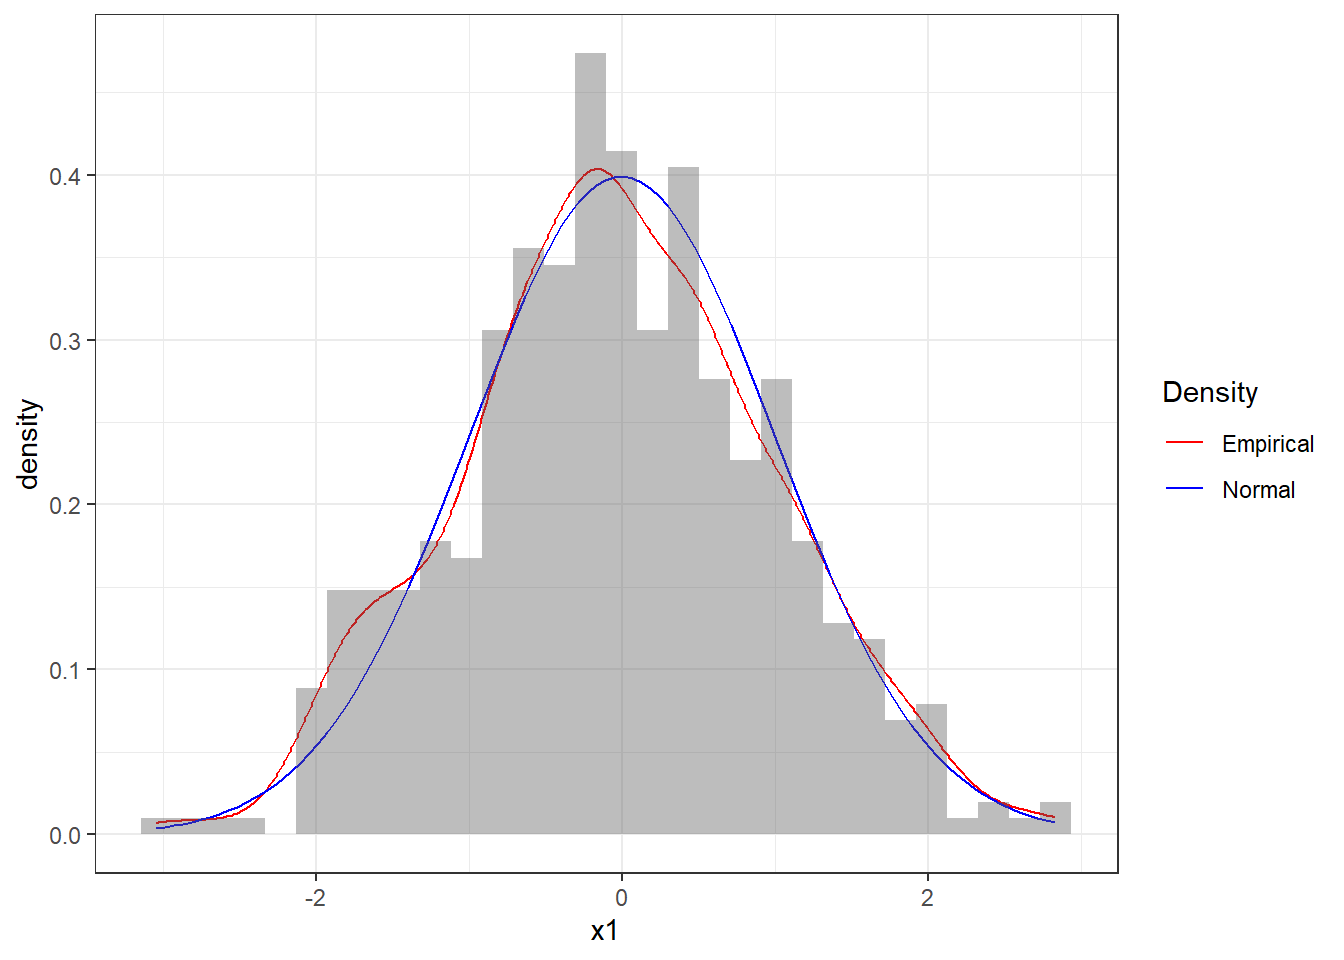
\includegraphics[width=0.5\linewidth]{SimBook_files/figure-latex/normhist-1} 

}

\caption{Histogram of the sequence x1 together with theoretical pdf of the standard Normal}\label{fig:normhist}
\end{figure}

Figure \ref{fig:normhist} reports the histogram of the sequence \texttt{x1} together with a smooth estimate of the histogram, often called density plot, in the red line. The blue line denotes the theoretical pdf of the standard Normal distribution. We can see that the sequence seems to follow quite closely a Normal distribution and therefore we could be convinced that the numbers are indeed Normal.

Let's consider a different sequence \texttt{x2}. Figure \ref{fig:exphist} clearly shows that there is a poor fit between the sequence and the standard Normal distribution. So we would in general not believe that these observations came from a Standard Normal.

\begin{Shaded}
\begin{Highlighting}[]
\FunctionTok{ggplot}\NormalTok{(x2, }\FunctionTok{aes}\NormalTok{(x2)) }\SpecialCharTok{+}
   \FunctionTok{geom\_line}\NormalTok{(}\FunctionTok{aes}\NormalTok{(}\AttributeTok{y =}\NormalTok{ ..density.., }\AttributeTok{colour =} \StringTok{\textquotesingle{}Empirical\textquotesingle{}}\NormalTok{), }\AttributeTok{stat =} \StringTok{\textquotesingle{}density\textquotesingle{}}\NormalTok{) }\SpecialCharTok{+}
   \FunctionTok{stat\_function}\NormalTok{(}\AttributeTok{fun =}\NormalTok{ dnorm, }\FunctionTok{aes}\NormalTok{(}\AttributeTok{colour =} \StringTok{\textquotesingle{}Normal\textquotesingle{}}\NormalTok{)) }\SpecialCharTok{+}      
   \FunctionTok{geom\_histogram}\NormalTok{(}\FunctionTok{aes}\NormalTok{(}\AttributeTok{y =}\NormalTok{ ..density..), }\AttributeTok{alpha =} \FloatTok{0.4}\NormalTok{) }\SpecialCharTok{+}      
   \FunctionTok{scale\_colour\_manual}\NormalTok{(}\AttributeTok{name =} \StringTok{\textquotesingle{}Density\textquotesingle{}}\NormalTok{, }\AttributeTok{values =} \FunctionTok{c}\NormalTok{(}\StringTok{\textquotesingle{}red\textquotesingle{}}\NormalTok{, }\StringTok{\textquotesingle{}blue\textquotesingle{}}\NormalTok{)) }\SpecialCharTok{+}
   \FunctionTok{theme\_bw}\NormalTok{()}
\end{Highlighting}
\end{Shaded}

\begin{figure}

{\centering 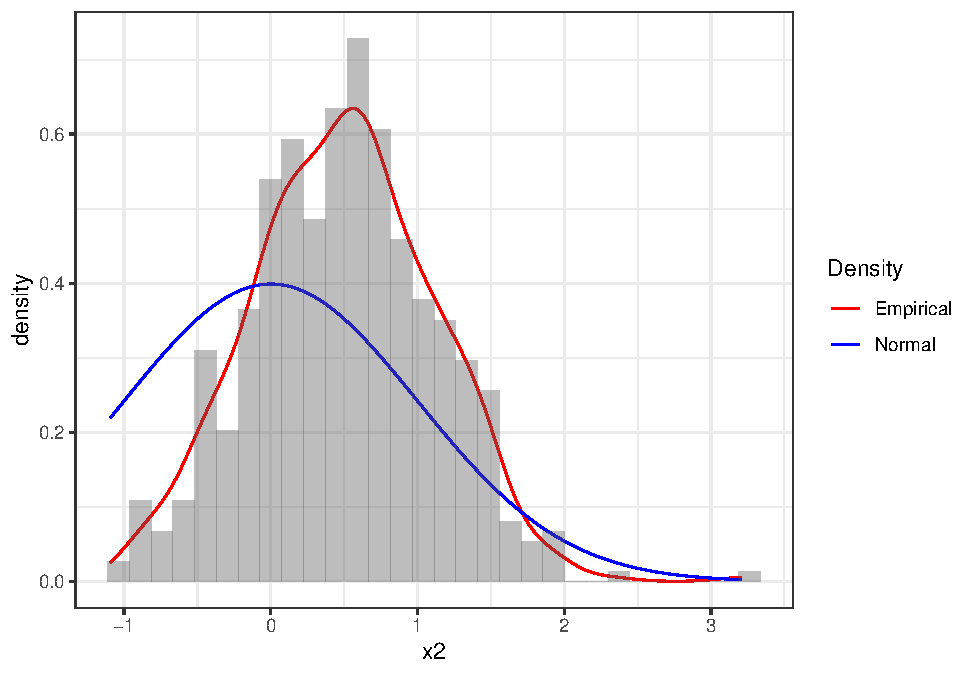
\includegraphics[width=0.5\linewidth]{SimBook_files/figure-latex/exphist-1} 

}

\caption{Histogram of the sequence x2 together with theoretical pdf of the standard Normal}\label{fig:exphist}
\end{figure}

\hypertarget{empirical-cumulative-distribution-function}{%
\subsubsection{Empirical Cumulative Distribution Function}\label{empirical-cumulative-distribution-function}}

We have already seen for uniform numbers that we can use the empirical cdf to assess if a sequence of numbers is uniformly distributed. We can use the exact same method for any other distribution.

Figure \ref{fig:normecdf} reports the ecdf of the sequence of numbers \texttt{x1} (in red) together with the theoretical cdf of the standard Normal (in blue). We can see that the two functions match closely and therefore we could assume that the sequence is distributed as a standard Normal.

\begin{Shaded}
\begin{Highlighting}[]
\FunctionTok{ggplot}\NormalTok{(x1, }\FunctionTok{aes}\NormalTok{(x1)) }\SpecialCharTok{+}
   \FunctionTok{stat\_ecdf}\NormalTok{(}\AttributeTok{geom =} \StringTok{"step"}\NormalTok{,}\FunctionTok{aes}\NormalTok{(}\AttributeTok{colour =} \StringTok{\textquotesingle{}Empirical\textquotesingle{}}\NormalTok{)) }\SpecialCharTok{+}
   \FunctionTok{stat\_function}\NormalTok{(}\AttributeTok{fun =}\NormalTok{ pnorm,}\FunctionTok{aes}\NormalTok{(}\AttributeTok{colour =} \StringTok{\textquotesingle{}Theoretical\textquotesingle{}}\NormalTok{)) }\SpecialCharTok{+}
   \FunctionTok{theme\_bw}\NormalTok{() }\SpecialCharTok{+}      
   \FunctionTok{scale\_colour\_manual}\NormalTok{(}\AttributeTok{name =} \StringTok{\textquotesingle{}Density\textquotesingle{}}\NormalTok{, }\AttributeTok{values =} \FunctionTok{c}\NormalTok{(}\StringTok{\textquotesingle{}red\textquotesingle{}}\NormalTok{, }\StringTok{\textquotesingle{}blue\textquotesingle{}}\NormalTok{))}
\end{Highlighting}
\end{Shaded}

\begin{figure}

{\centering 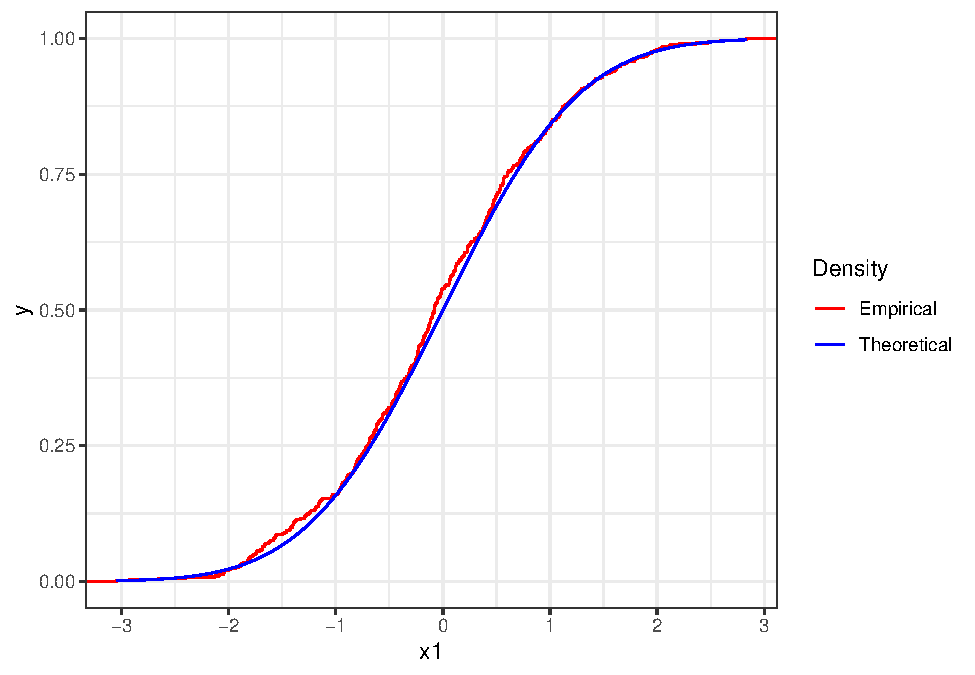
\includegraphics[width=0.5\linewidth]{SimBook_files/figure-latex/normecdf-1} 

}

\caption{Empirical cdf the sequence x1 together with theoretical cdf of the standard Normal}\label{fig:normecdf}
\end{figure}

Figure \ref{fig:expecdf} reports the same plot but for the sequence \texttt{x2}. The two lines strongly differ and therefore it cannot be assume that the sequence is distributed as a standard Normal.

\begin{Shaded}
\begin{Highlighting}[]
\FunctionTok{ggplot}\NormalTok{(x2, }\FunctionTok{aes}\NormalTok{(x2)) }\SpecialCharTok{+}
   \FunctionTok{stat\_ecdf}\NormalTok{(}\AttributeTok{geom =} \StringTok{"step"}\NormalTok{,}\FunctionTok{aes}\NormalTok{(}\AttributeTok{colour =} \StringTok{\textquotesingle{}Empirical\textquotesingle{}}\NormalTok{)) }\SpecialCharTok{+}
   \FunctionTok{stat\_function}\NormalTok{(}\AttributeTok{fun =}\NormalTok{ pnorm,}\FunctionTok{aes}\NormalTok{(}\AttributeTok{colour =} \StringTok{\textquotesingle{}Theoretical\textquotesingle{}}\NormalTok{)) }\SpecialCharTok{+}
   \FunctionTok{theme\_bw}\NormalTok{() }\SpecialCharTok{+}      
   \FunctionTok{scale\_colour\_manual}\NormalTok{(}\AttributeTok{name =} \StringTok{\textquotesingle{}Density\textquotesingle{}}\NormalTok{, }\AttributeTok{values =} \FunctionTok{c}\NormalTok{(}\StringTok{\textquotesingle{}red\textquotesingle{}}\NormalTok{, }\StringTok{\textquotesingle{}blue\textquotesingle{}}\NormalTok{))}
\end{Highlighting}
\end{Shaded}

\begin{figure}

{\centering 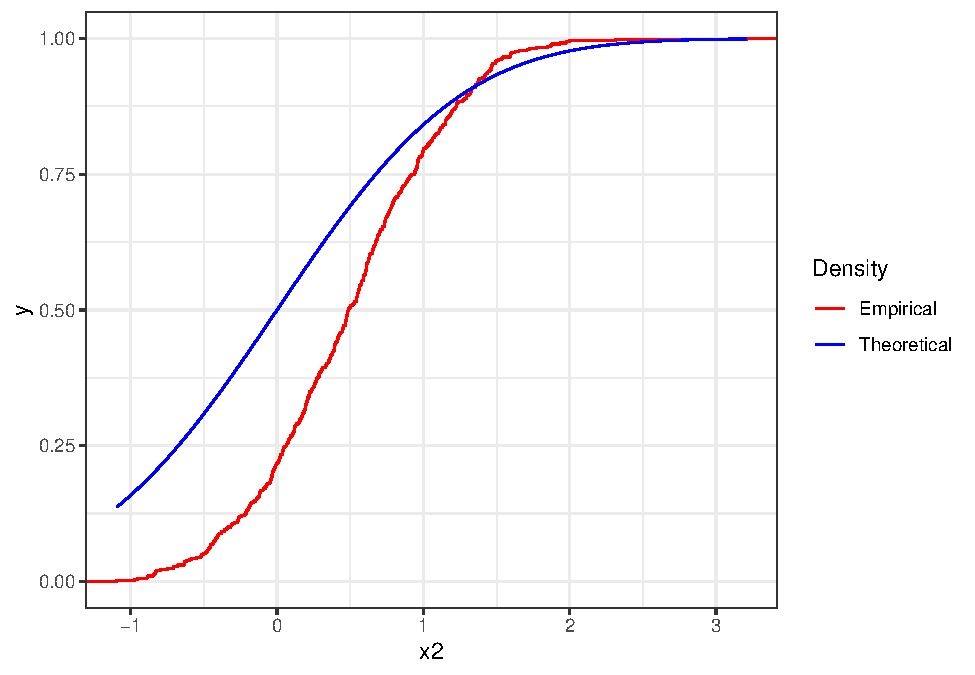
\includegraphics[width=0.5\linewidth]{SimBook_files/figure-latex/expecdf-1} 

}

\caption{Empirical cdf the sequence x2 together with theoretical cdf of the standard Normal}\label{fig:expecdf}
\end{figure}

\hypertarget{qq-plot}{%
\subsubsection{QQ-Plot}\label{qq-plot}}

A third visualization of the distribution of a sequence of numbers is the so called \emph{QQ-plot}. You may have already seen this when checking if the residuals of a linear regression follow a Normal distribution. But more generally, qq-plots can be used to check if a sequence of numbers is distributed according to any distribution.

We will not the details about how these are constructed but just their interpretation and implementation. Let's consider Figure \ref{fig:qqnorm}. The plot is composed of a series of points, where each point is associated to a number in our random sequence, and a line, which describes the theoretical distribution we are targeting. The closest the points and the line are, the better the fit to that distribution.

In particular, in Figure \ref{fig:qqnorm} we are checking if the sequence \texttt{x1} is distributed according to a standard Normal (represented by the straight line). Since the points are placed almost in a straight line over the theoretical line of the standard Normal, we can assume the sequence to be Normal.

\begin{Shaded}
\begin{Highlighting}[]
\FunctionTok{ggplot}\NormalTok{(x1, }\FunctionTok{aes}\NormalTok{(}\AttributeTok{sample =}\NormalTok{ x1)) }\SpecialCharTok{+}
   \FunctionTok{stat\_qq}\NormalTok{(}\AttributeTok{distribution =}\NormalTok{ qnorm) }\SpecialCharTok{+}
   \FunctionTok{stat\_qq\_line}\NormalTok{(}\AttributeTok{distribution =}\NormalTok{ qnorm) }\SpecialCharTok{+}
   \FunctionTok{theme\_bw}\NormalTok{()}
\end{Highlighting}
\end{Shaded}

\begin{figure}

{\centering 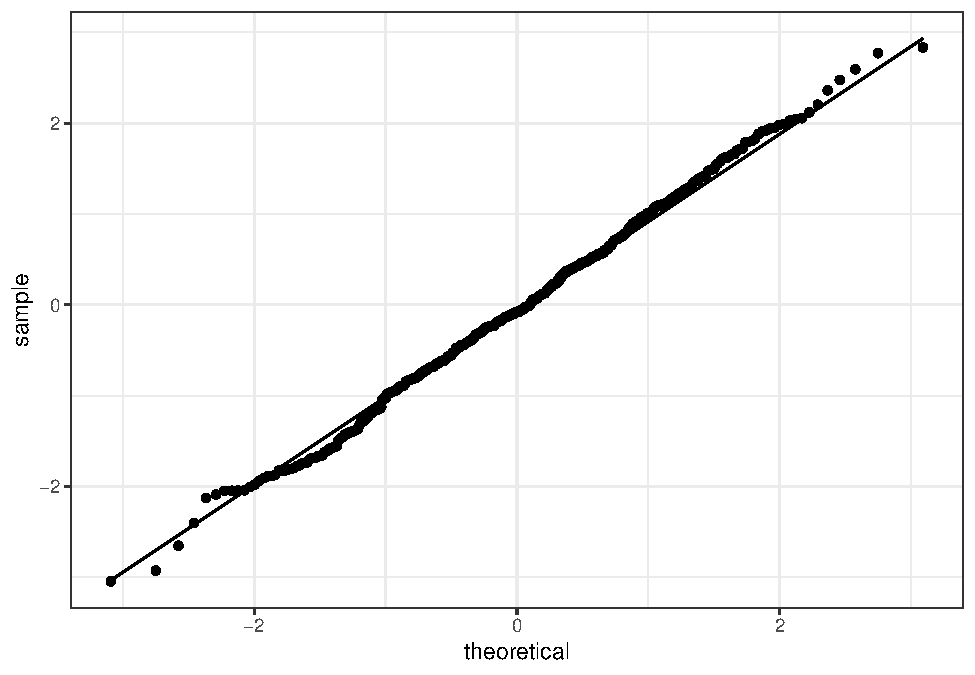
\includegraphics[width=0.5\linewidth]{SimBook_files/figure-latex/qqnorm-1} 

}

\caption{QQ-plot for the sequence x1 checking against the standard Normal}\label{fig:qqnorm}
\end{figure}

Figure \ref{fig:qqexp} reports the qq-plot for the sequence \texttt{x2} to check if the data can be following a standard Normal. We can see that the points do not differ too much from the straight line and in this case we could assume the data to be Normal (notice that the histograms and the cdf strongly suggested that this sequence was not Normal).

\begin{Shaded}
\begin{Highlighting}[]
\FunctionTok{ggplot}\NormalTok{(x2, }\FunctionTok{aes}\NormalTok{(}\AttributeTok{sample =}\NormalTok{ x2)) }\SpecialCharTok{+}
   \FunctionTok{stat\_qq}\NormalTok{(}\AttributeTok{distribution =}\NormalTok{ qnorm) }\SpecialCharTok{+}
   \FunctionTok{stat\_qq\_line}\NormalTok{(}\AttributeTok{distribution =}\NormalTok{ qnorm) }\SpecialCharTok{+}
   \FunctionTok{theme\_bw}\NormalTok{()}
\end{Highlighting}
\end{Shaded}

\begin{figure}

{\centering 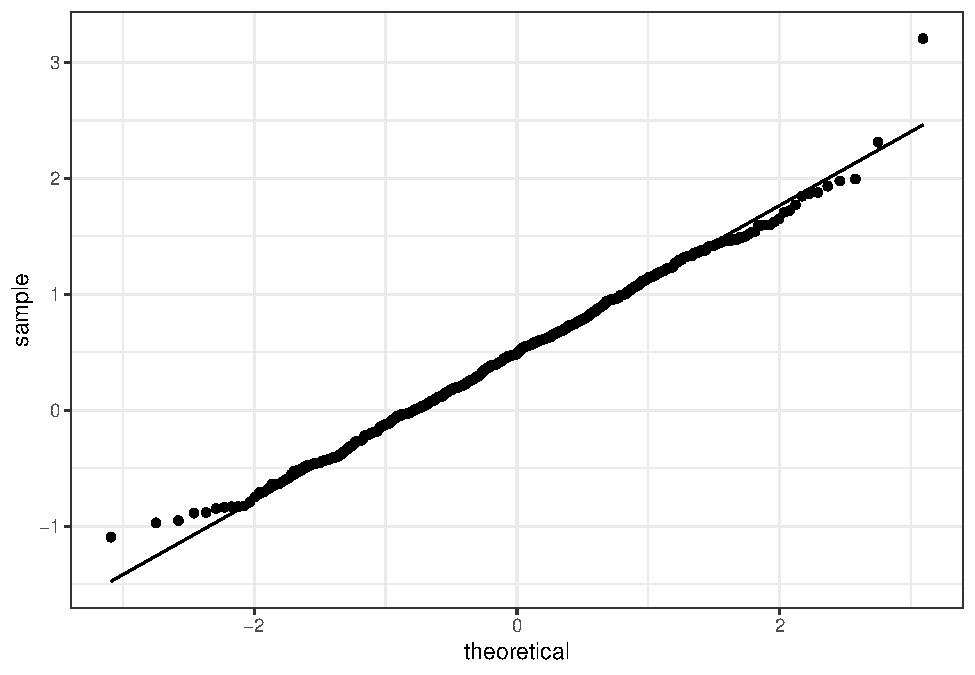
\includegraphics[width=0.5\linewidth]{SimBook_files/figure-latex/qqexp-1} 

}

\caption{QQ-plot for the sequence x2 checking against the standard Normal}\label{fig:qqexp}
\end{figure}

Notice that the form of the qq-plot does not only depend on the sequence of numbers we are considering, but also on the distribution we are testing it against. Figure \ref{fig:qqnorm} reports the qq-plot for the sequence \texttt{x1} when checked against an Exponential random variable with parameter \(\lambda =3\). Given that the sequence also includes negative numbers, it does not make sense to check if it is distributed as an Exponential (since it can only model non-negative data), but this is just an illustration.

\begin{Shaded}
\begin{Highlighting}[]
\FunctionTok{ggplot}\NormalTok{(x1, }\FunctionTok{aes}\NormalTok{(}\AttributeTok{sample =}\NormalTok{ x1)) }\SpecialCharTok{+}
   \FunctionTok{stat\_qq}\NormalTok{(}\AttributeTok{distribution =}\NormalTok{ qexp, }\AttributeTok{dparams =}\NormalTok{ (}\AttributeTok{rate =} \DecValTok{3}\NormalTok{)) }\SpecialCharTok{+}
   \FunctionTok{stat\_qq\_line}\NormalTok{(}\AttributeTok{distribution =}\NormalTok{ qexp, }\AttributeTok{dparams =}\NormalTok{ (}\AttributeTok{rate =} \DecValTok{3}\NormalTok{)) }\SpecialCharTok{+}
   \FunctionTok{theme\_bw}\NormalTok{()}
\end{Highlighting}
\end{Shaded}

\begin{figure}

{\centering 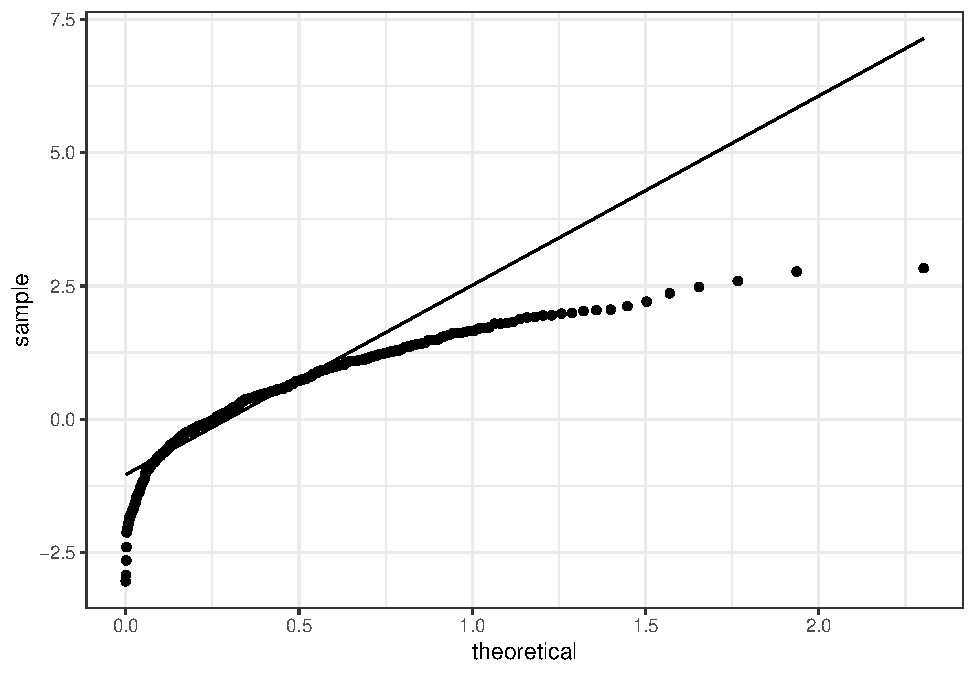
\includegraphics[width=0.5\linewidth]{SimBook_files/figure-latex/qqnorm1-1} 

}

\caption{QQ-plot for the sequence x1 checking against an Exponential}\label{fig:qqnorm1}
\end{figure}

\hypertarget{formal-testing}{%
\subsubsection{Formal Testing}\label{formal-testing}}

The above plots are highly informative since they provide insights into the shape of the data distribution, but these are not formal. Again, we can carry out tests of hypothesis to check if data is distributed as a specific random variable, just like we did for the Uniform.

Again, there are many tests one could use, but here we focus only on the Kolmogorov-Smirnov Test which checks how close the empirical and the theoretical cdfs are. It is implemented in the \texttt{ks.test} R function.

Let's check if the sequences \texttt{x1} and \texttt{x2} are distributed as a standard Normal.

\begin{Shaded}
\begin{Highlighting}[]
\FunctionTok{ks.test}\NormalTok{(x1,pnorm)}
\end{Highlighting}
\end{Shaded}

\begin{verbatim}
## 
##  One-sample Kolmogorov-Smirnov test
## 
## data:  x1
## D = 0.041896, p-value = 0.3439
## alternative hypothesis: two-sided
\end{verbatim}

\begin{Shaded}
\begin{Highlighting}[]
\FunctionTok{ks.test}\NormalTok{(x2,pnorm)}
\end{Highlighting}
\end{Shaded}

\begin{verbatim}
## 
##  One-sample Kolmogorov-Smirnov test
## 
## data:  x2
## D = 0.2997, p-value < 2.2e-16
## alternative hypothesis: two-sided
\end{verbatim}

The conclusion is that \texttt{x1} is distributed as a standard Normal since the p-value of the test is large and for instance bigger than 0.10. On the other hand, the p-value for the Kolmogorov-Smirnov test over the sequence \texttt{x2} has a very small p-value thus leading us to reject the null hypothesis that the sequence is Normally distributed.

Notice that we can add extra inputs to the function. For instance we can check if \texttt{x1} is distributed as a Normal with \texttt{mean\ =\ 2} and \texttt{sd\ =\ 2} using:

\begin{Shaded}
\begin{Highlighting}[]
\FunctionTok{ks.test}\NormalTok{(x1, pnorm, }\AttributeTok{mean =} \DecValTok{2}\NormalTok{, }\AttributeTok{sd =} \DecValTok{2}\NormalTok{)}
\end{Highlighting}
\end{Shaded}

\begin{verbatim}
## 
##  One-sample Kolmogorov-Smirnov test
## 
## data:  x1
## D = 0.54604, p-value < 2.2e-16
## alternative hypothesis: two-sided
\end{verbatim}

The p-value is small and therefore we would reject the null hypothesis that the sequence is distributed as a Normal with mean two and standard deviation two.

\hypertarget{testing-independence-1}{%
\subsection{Testing Independence}\label{testing-independence-1}}

The other step in assessing if a sequence of numbers is pseudo-random is checking if independence holds. We have already learned that one possible way to do this is by computing the auto-correlation function with the R function \texttt{acf}. Let's compute the auto-correlations of various lags for the sequences \texttt{x1} and \texttt{x2}, reported in Figure \ref{fig:acf12}. We can see that for \texttt{x2} all bars are within the confidence bands (recall that the first bar for lag \(k=0\) should not be considered). For \texttt{x1} the bar corresponding to lag 1 is slightly outside the confidence bands, indicating that there may be some dependence.

\begin{Shaded}
\begin{Highlighting}[]
\FunctionTok{acf}\NormalTok{(x1)}
\FunctionTok{acf}\NormalTok{(x2)}
\end{Highlighting}
\end{Shaded}

\begin{figure}

{\centering 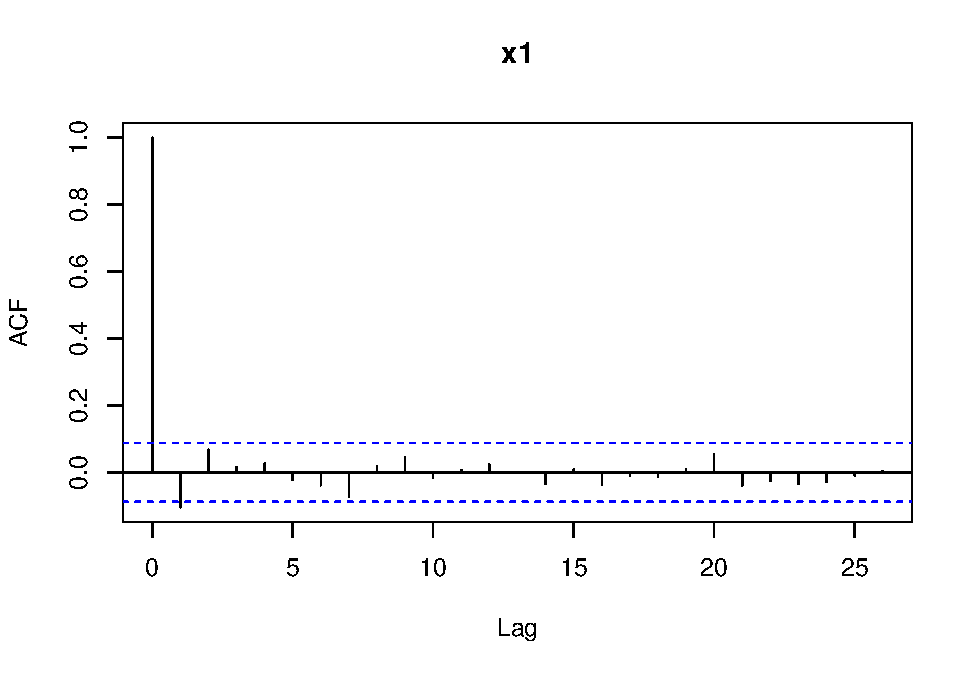
\includegraphics[width=0.5\linewidth]{SimBook_files/figure-latex/acf12-1} 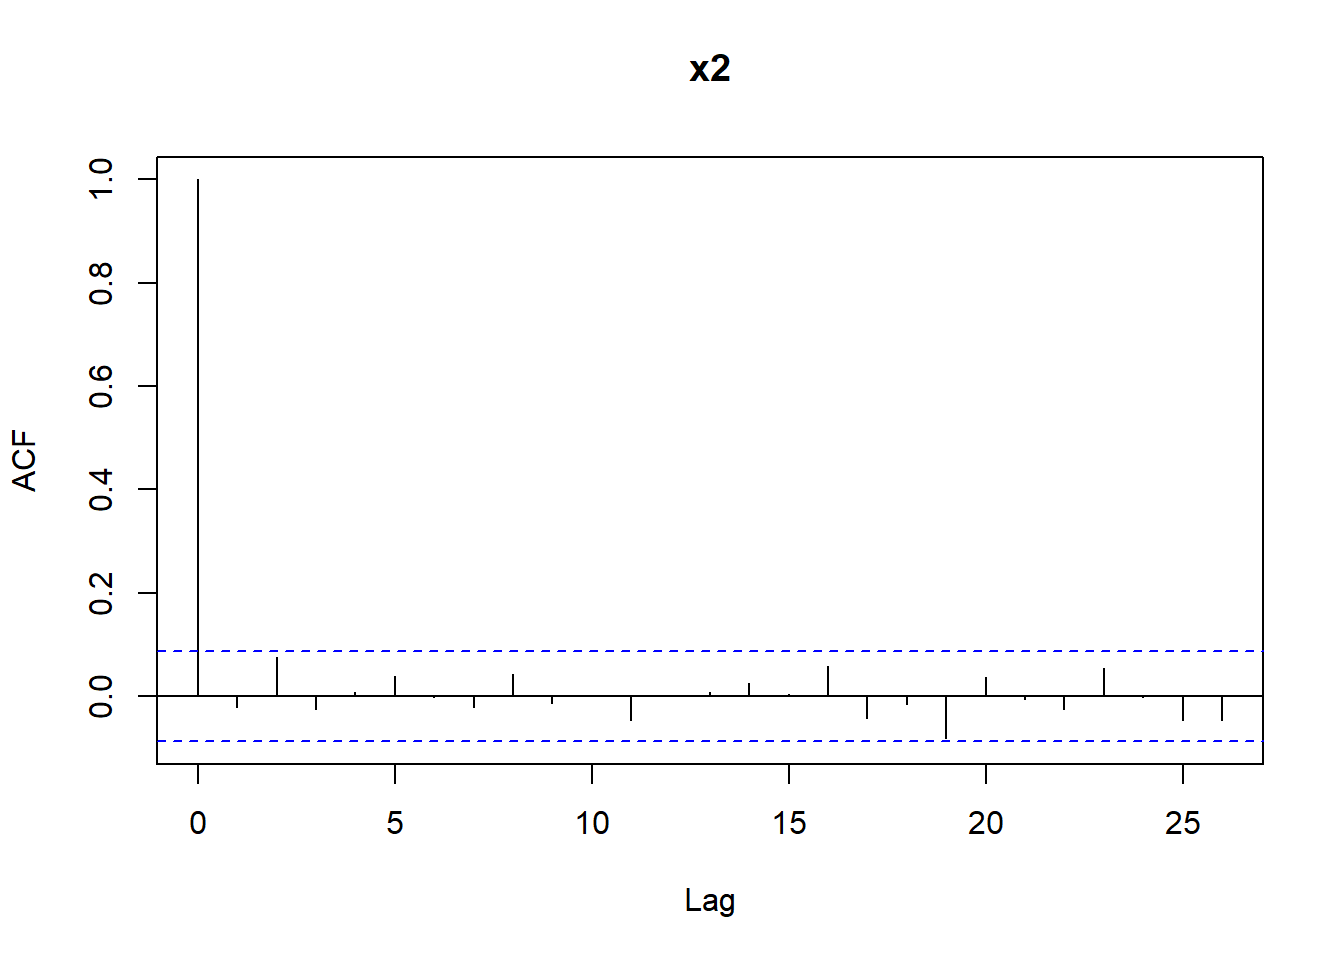
\includegraphics[width=0.5\linewidth]{SimBook_files/figure-latex/acf12-2} 

}

\caption{Autocorrelations for the sequences x1 and x2.}\label{fig:acf12}
\end{figure}

Let's run the Box test to assess if the assumption of independence is tenable for both sequences.

\begin{Shaded}
\begin{Highlighting}[]
\FunctionTok{Box.test}\NormalTok{(x1, }\AttributeTok{lag =} \DecValTok{5}\NormalTok{)}
\end{Highlighting}
\end{Shaded}

\begin{verbatim}
## 
##  Box-Pierce test
## 
## data:  x1
## X-squared = 8.4212, df = 5, p-value = 0.1345
\end{verbatim}

\begin{Shaded}
\begin{Highlighting}[]
\FunctionTok{Box.test}\NormalTok{(x2, }\AttributeTok{lag =} \DecValTok{5}\NormalTok{)}
\end{Highlighting}
\end{Shaded}

\begin{verbatim}
## 
##  Box-Pierce test
## 
## data:  x2
## X-squared = 4.2294, df = 5, p-value = 0.5169
\end{verbatim}

In both cases the p-values are larger than 0.10, thus we would not reject the null hypothesis of independence for both sequences. Recall that \texttt{x1} is distributed as a standard Normal, whilst \texttt{x2} is not.

For the sequence \texttt{x1} we observed that one bar was slightly outside the confidence bands: this sometimes happens even when data is actually (pseudo-) random - I created \texttt{x1} using \texttt{rnorm}. The autocorrelations below are an instance of a case where independence is not tenable since we see that multiple bars are outside the confidence bands.

\begin{center}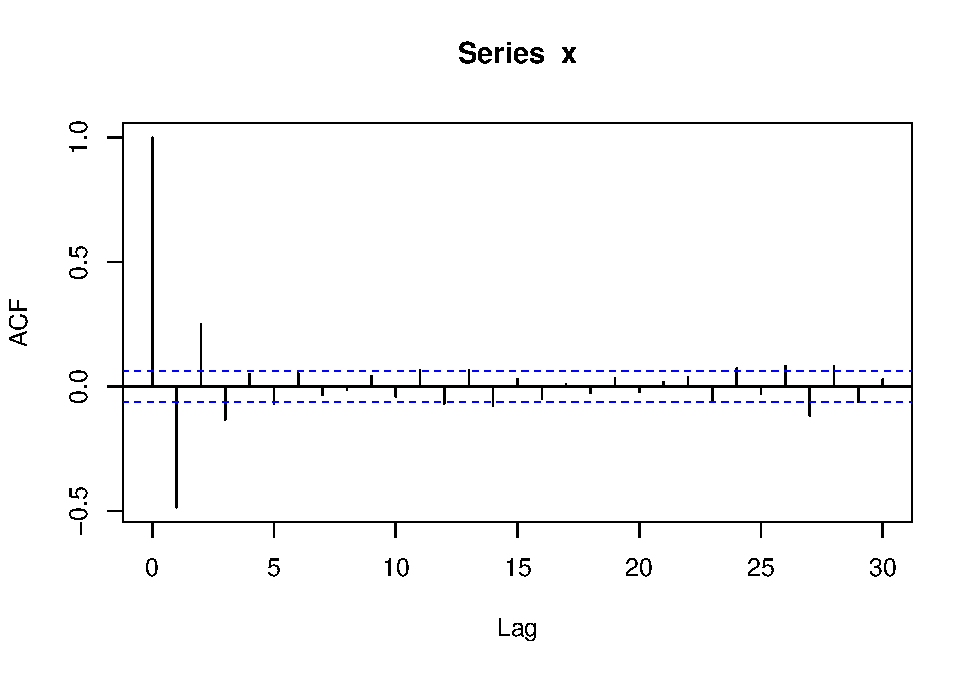
\includegraphics[width=0.5\linewidth]{SimBook_files/figure-latex/unnamed-chunk-93-1} \end{center}

\hypertarget{monte-carlo-simulation}{%
\chapter{Monte Carlo Simulation}\label{monte-carlo-simulation}}

The previous chapters laid the foundations of probability and statistics that now allow us to carry out meaningful simulation experiments. In this chapter we start looking at non-dynamic simulations which are often referred to as \emph{Monte Carlo simulations}.

\hypertarget{what-does-monte-carlo-simulation-mean}{%
\section{What does Monte Carlo simulation mean?}\label{what-does-monte-carlo-simulation-mean}}

The definition of the Monte Carlo concept can be a bit confusing. For this reason, we will take \emph{Sawilowsky's} example and distinguish between: Simulation, Monte Carlo method and Monte Carlo simulation.

\begin{itemize}
\item
  A \textbf{Simulation} is a fictitious representation of reality. For example: Drawing one pseudo-random uniform variable from the interval {[}0,1{]} can be used to simulate the tossing of a coin. If the value is less than or equal to 0.50 designate the outcome as heads, but if the value is greater than 0.50 designate the outcome as tails. This is a simulation, but not a Monte Carlo simulation.
\item
  A \textbf{Monte Carlo method} is a technique that can be used to solve a mathematical or statistical problem. For example: Pouring out a box of coins on a table, and then computing the ratio of coins that land heads versus tails is a Monte Carlo method of determining the behavior of repeated coin tosses, but it is not a simulation.
\item
  A \textbf{Monte Carlo simulation} uses repeated sampling to obtain the statistical properties of some phenomenon (or behavior). For example: drawing a large number of pseudo-random uniform variables from the interval {[}0,1{]} at one time, or once at many different times, and assigning values less than or equal to 0.50 as heads and greater than 0.50 as tails, is a Monte Carlo simulation of the behavior of repeatedly tossing a coin.
\end{itemize}

The main idea behind this method is that a phenomenon is simulated multiple times on a computer using random-number generation based and the results are aggregated to provide statistical summaries associated to the phenomenon.

Sawilowsky lists the characteristics of a high-quality Monte Carlo simulation:

\begin{itemize}
\item
  the (pseudo-random) number generator has certain characteristics (e.g.~a long ``period'' before the sequence repeats)
\item
  the (pseudo-random) number generator produces values that pass tests for randomness
\item
  there are enough samples to ensure accurate results
\item
  the algorithm used is valid for what is being modeled
\item
  it simulates the phenomenon in question.
\end{itemize}

\hypertarget{a-bit-of-history}{%
\section{A bit of history}\label{a-bit-of-history}}

There were several approaches to the Monte Carlo method in the early 20th century, but it was in the mid-1940s during the Manhattan Project at ``Los Alamos'' that this method was first intentionally developed by Stanislaw Ulam and John von Neumann for early work relating to the development of nuclear weapons.

Below you can read a quote from Stanislaw Ulam in which he explains how he came up with this simple but powerful method:

\begin{quote}
The first thoughts and attempts I made to practice {[}the Monte Carlo Method{]} were suggested by a question which occurred to me in 1946 as I was convalescing from an illness and playing solitaires. The question was what are the chances that a Canfield solitaire laid out with 52 cards will come out successfully? After spending a lot of time trying to estimate them by pure combinatorial calculations, I wondered whether a more practical method than ``abstract thinking'' might not be to lay it out say one hundred times and simply observe and count the number of successful plays. This was already possible to envisage with the beginning of the new era of fast computers, and I immediately thought of problems of neutron diffusion and other questions of mathematical physics, and more generally how to change processes described by certain differential equations into an equivalent form interpretable as a succession of random operations. Later {[}in 1946{]}, I described the idea to John von Neumann, and we began to plan actual calculations.
\end{quote}

Being secret, the work of von Neumann and Ulam required a code name. A colleague of von Neumann and Ulam, Nicholas Metropolis, suggested using the name Monte Carlo, which refers to the Monte Carlo Casino in Monaco where Ulam's uncle would borrow money from relatives to gamble.

\hypertarget{steps-of-monte-carlo-simulation}{%
\section{Steps of Monte Carlo simulation}\label{steps-of-monte-carlo-simulation}}

Monte Carlo methods vary, but tend to follow a particular pattern:

\begin{enumerate}
\def\labelenumi{\arabic{enumi}.}
\item
  Define a domain of possible inputs
\item
  Generate inputs randomly from a probability distribution over the domain
\item
  Perform a deterministic computation on the inputs
\item
  Aggregate the results
\end{enumerate}

To better understand how Monte Carlo simulation works we will develop a classic experiment: The \(\pi\) number estimation.

\(\pi\) is the mathematical constant, which is equal to 3.14159265\ldots, defined as the ratio of a circle's circumference to its diameter. It has been calculated in hundreds of different ways over the years. Today, with computational advances, a very useful way is through Monte Carlo Simulation.

Consider a circle with radius \(r\), which is fixed and known.

\begin{center}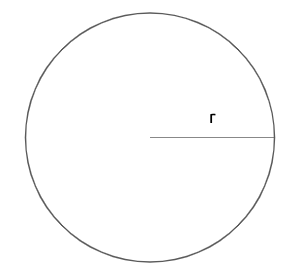
\includegraphics[width=0.25\linewidth]{images/Circle-radio} \end{center}

Imagine that this circle is circumscribed within a square, which therefore has side \(2r\) (also equal to the diameter).

\begin{center}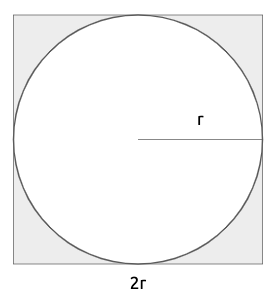
\includegraphics[width=0.25\linewidth]{images/Circle-square} \end{center}

What is the probability that if I choose a random point inside the square, it will also be inside the circle? If I choose any random point within the square, it can be inside the circle or just inside the square. A very simple way to compute this probability is the ratio between the area of the circle and the area of the square.

\[
P(point\ inside\ the\ circle) = \frac{area\ of\ the\ circle}{area\ of\ the\ square}=\frac{\pi r^2}{2r\times 2r}=\frac{\pi}{4}
\]

The probability that a random selected point in the square is in the circle is \(\pi/4\). This means that if I were to replicate the selection of a random point in the square a large number of times, I could count the proportion of points inside the circle, multiply it by four and that would give me an approximation of \(\pi\).

We will create a Monte Carlo experiment in R which implements the ideas above. We will carry out the experiment in 5 steps:

\begin{enumerate}
\def\labelenumi{\arabic{enumi}.}
\item
  Generate 2 random numbers between -1 and 1 in total 100 times (\(x\) and \(y\)).
\item
  Calculate \(x^2 + y^2\) (This is the circumference equation).

  \begin{itemize}
  \tightlist
  \item
    If the value is less than 1, the case will be inside the circle
  \item
    If the value is greater than 1, the case will be outside the circle.
  \end{itemize}
\item
  Calculate the proportion of points inside the circle and multiply it by four to approximate the \(\pi\) value.
\item
  Repeat the experiment a thousand times, to get different approximations to \(\pi\).
\item
  Calculate the average of the previous 1000 experiments to give a final value estimate.
\end{enumerate}

\hypertarget{estimating-pi-step-1}{%
\subsection{\texorpdfstring{Estimating \(\pi\): step 1}{Estimating \textbackslash pi: step 1}}\label{estimating-pi-step-1}}

Generate two random numbers between -1 and 1, 100 times:

\begin{Shaded}
\begin{Highlighting}[]
\FunctionTok{set.seed}\NormalTok{(}\DecValTok{2021}\NormalTok{)}
\NormalTok{nPoints }\OtherTok{\textless{}{-}} \DecValTok{100}
\NormalTok{x }\OtherTok{\textless{}{-}} \FunctionTok{runif}\NormalTok{(nPoints,}\SpecialCharTok{{-}}\DecValTok{1}\NormalTok{,}\DecValTok{1}\NormalTok{)}
\NormalTok{y }\OtherTok{\textless{}{-}} \FunctionTok{runif}\NormalTok{(nPoints,}\SpecialCharTok{{-}}\DecValTok{1}\NormalTok{,}\DecValTok{1}\NormalTok{)}
\FunctionTok{head}\NormalTok{(x)}
\end{Highlighting}
\end{Shaded}

\begin{verbatim}
## [1] -0.09746527  0.56755957  0.41936446 -0.23651148  0.27264754  0.40269205
\end{verbatim}

\begin{Shaded}
\begin{Highlighting}[]
\FunctionTok{head}\NormalTok{(y)}
\end{Highlighting}
\end{Shaded}

\begin{verbatim}
## [1] -0.38312966 -0.42837094 -0.97592119  0.76677917  0.03488941 -0.53043372
\end{verbatim}

So both \texttt{x} and \texttt{y} are vectors of length 100 storing numbers between -1 and 1.

\hypertarget{estimating-pi-step-2}{%
\subsection{\texorpdfstring{Estimating \(\pi\): step 2}{Estimating \textbackslash pi: step 2}}\label{estimating-pi-step-2}}

Calculate the circumference equation.

\begin{itemize}
\tightlist
\item
  If the value is less than 1, the case will be inside the circle
\item
  If the value is greater than 1, the case will be outside the circle.
\end{itemize}

\begin{Shaded}
\begin{Highlighting}[]
\NormalTok{result }\OtherTok{\textless{}{-}} \FunctionTok{ifelse}\NormalTok{(x}\SpecialCharTok{\^{}}\DecValTok{2} \SpecialCharTok{+}\NormalTok{ y}\SpecialCharTok{\^{}}\DecValTok{2} \SpecialCharTok{\textless{}=} \DecValTok{1}\NormalTok{, }\ConstantTok{TRUE}\NormalTok{, }\ConstantTok{FALSE}\NormalTok{)}
\FunctionTok{head}\NormalTok{(result)}
\end{Highlighting}
\end{Shaded}

\begin{verbatim}
## [1]  TRUE  TRUE FALSE  TRUE  TRUE  TRUE
\end{verbatim}

The vector \texttt{result} has in i-th position \texttt{TRUE} if \texttt{x{[}i{]}\^{}2\ +\ y{[}i{]}\^{}2\ \textless{}=\ 1}, that is if the associated point is within the circle. We can see that out of the first six simulated points, only one is outside the circle.

\hypertarget{estimating-pi-step-3}{%
\subsection{\texorpdfstring{Estimating \(\pi\): step 3}{Estimating \textbackslash pi: step 3}}\label{estimating-pi-step-3}}

Calculate the proportion of points inside the circle and multiply it by four to approximate the \(\pi\) value.

\begin{Shaded}
\begin{Highlighting}[]
\DecValTok{4}\SpecialCharTok{*}\FunctionTok{sum}\NormalTok{(result)}\SpecialCharTok{/}\NormalTok{nPoints}
\end{Highlighting}
\end{Shaded}

\begin{verbatim}
## [1] 2.92
\end{verbatim}

So using our 100 simulated points, we came up with an approximation of 2.92 for the value of \(\pi\). Of course this number depends on the random numbers that were generated. If we were to repeat it, we would get a different approximation.

\begin{Shaded}
\begin{Highlighting}[]
\FunctionTok{set.seed}\NormalTok{(}\DecValTok{1988}\NormalTok{)}
\NormalTok{x }\OtherTok{\textless{}{-}} \FunctionTok{runif}\NormalTok{(nPoints,}\SpecialCharTok{{-}}\DecValTok{1}\NormalTok{,}\DecValTok{1}\NormalTok{)}
\NormalTok{y }\OtherTok{\textless{}{-}} \FunctionTok{runif}\NormalTok{(nPoints,}\SpecialCharTok{{-}}\DecValTok{1}\NormalTok{,}\DecValTok{1}\NormalTok{)}
\NormalTok{result }\OtherTok{\textless{}{-}} \FunctionTok{ifelse}\NormalTok{(x}\SpecialCharTok{\^{}}\DecValTok{2} \SpecialCharTok{+}\NormalTok{ y}\SpecialCharTok{\^{}}\DecValTok{2} \SpecialCharTok{\textless{}=} \DecValTok{1}\NormalTok{, }\ConstantTok{TRUE}\NormalTok{, }\ConstantTok{FALSE}\NormalTok{)}
\DecValTok{4}\SpecialCharTok{*}\FunctionTok{sum}\NormalTok{(result)}\SpecialCharTok{/}\NormalTok{nPoints}
\end{Highlighting}
\end{Shaded}

\begin{verbatim}
## [1] 3.08
\end{verbatim}

\hypertarget{estimating-pi-step-4}{%
\subsection{\texorpdfstring{Estimating \(\pi\): step 4}{Estimating \textbackslash pi: step 4}}\label{estimating-pi-step-4}}

Repeat the experiment a thousand times, to get different approximations to \(\pi\).

We could do this by coding a \texttt{for} cycle, but we will take advantage of some features already implemented in R. In order to do this however, we first need to define a function which repeats our estimation of \(\pi\) given 100 random points.

\begin{Shaded}
\begin{Highlighting}[]
\NormalTok{piVal }\OtherTok{\textless{}{-}} \ControlFlowTok{function}\NormalTok{(}\AttributeTok{nPoints =} \DecValTok{100}\NormalTok{)\{}
\NormalTok{  x }\OtherTok{\textless{}{-}} \FunctionTok{runif}\NormalTok{(nPoints,}\SpecialCharTok{{-}}\DecValTok{1}\NormalTok{,}\DecValTok{1}\NormalTok{)}
\NormalTok{  y }\OtherTok{\textless{}{-}} \FunctionTok{runif}\NormalTok{(nPoints,}\SpecialCharTok{{-}}\DecValTok{1}\NormalTok{,}\DecValTok{1}\NormalTok{)}
\NormalTok{  result }\OtherTok{\textless{}{-}} \FunctionTok{ifelse}\NormalTok{(x}\SpecialCharTok{\^{}}\DecValTok{2}\SpecialCharTok{+}\NormalTok{y}\SpecialCharTok{\^{}}\DecValTok{2} \SpecialCharTok{\textless{}=} \DecValTok{1}\NormalTok{, }\ConstantTok{TRUE}\NormalTok{, }\ConstantTok{FALSE}\NormalTok{)}
  \DecValTok{4}\SpecialCharTok{*}\FunctionTok{sum}\NormalTok{(result)}\SpecialCharTok{/}\NormalTok{nPoints}
\NormalTok{\}}

\FunctionTok{set.seed}\NormalTok{(}\DecValTok{2021}\NormalTok{)}
\FunctionTok{piVal}\NormalTok{()}
\end{Highlighting}
\end{Shaded}

\begin{verbatim}
## [1] 2.92
\end{verbatim}

\begin{Shaded}
\begin{Highlighting}[]
\FunctionTok{set.seed}\NormalTok{(}\DecValTok{1988}\NormalTok{)}
\FunctionTok{piVal}\NormalTok{()}
\end{Highlighting}
\end{Shaded}

\begin{verbatim}
## [1] 3.08
\end{verbatim}

So we can see that the function works since it gives us the same output as the code above.

Now we can use the function \texttt{replicate} in R, to replicate the experiment 1000 times, or to put it differently, to compute the function \texttt{piVal} 1000 times. \texttt{replicate} takes two inputs:

\begin{itemize}
\item
  \texttt{n}: the number of times we want to replicate the experimet;
\item
  \texttt{expr}: the function we want to be replicated
\end{itemize}

Therefore the following code replicates the experiment:

\begin{Shaded}
\begin{Highlighting}[]
\FunctionTok{set.seed}\NormalTok{(}\DecValTok{2021}\NormalTok{)}
\NormalTok{N }\OtherTok{\textless{}{-}} \DecValTok{1000}
\NormalTok{pis }\OtherTok{\textless{}{-}} \FunctionTok{replicate}\NormalTok{(N, }\FunctionTok{piVal}\NormalTok{())}
\FunctionTok{head}\NormalTok{(pis)}
\end{Highlighting}
\end{Shaded}

\begin{verbatim}
## [1] 2.92 3.20 3.16 3.08 3.20 2.76
\end{verbatim}

We can see that the first entry of the vector \texttt{pis} is indeed \texttt{pis{[}1{]}} which is the same value we obtained running the function ourselves (in both cases we fixed the same seed).

\hypertarget{estimating-pi-step-5}{%
\subsection{\texorpdfstring{Estimating \(\pi\): step 5}{Estimating \textbackslash pi: step 5}}\label{estimating-pi-step-5}}

Calculate the average of the previous 1000 experiments to give a final value estimate.

\begin{Shaded}
\begin{Highlighting}[]
\FunctionTok{mean}\NormalTok{(pis)}
\end{Highlighting}
\end{Shaded}

\begin{verbatim}
## [1] 3.13828
\end{verbatim}

The average gives us a good approximation of \(\pi\).

A boxplot can give us a visualization of the results.

\begin{Shaded}
\begin{Highlighting}[]
\FunctionTok{boxplot}\NormalTok{(pis)}
\end{Highlighting}
\end{Shaded}

\begin{center}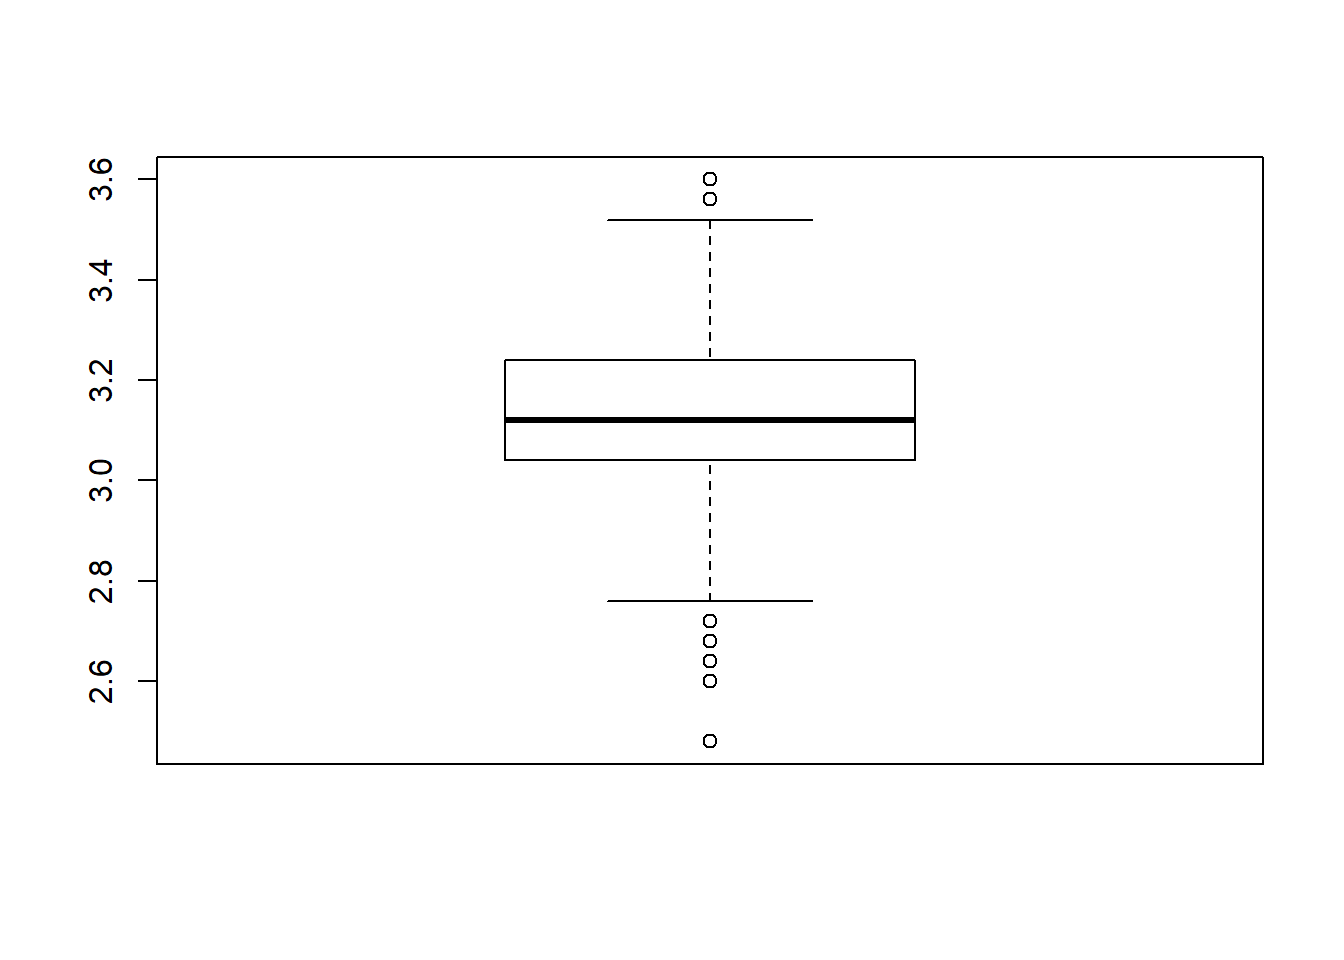
\includegraphics[width=0.5\linewidth]{SimBook_files/figure-latex/unnamed-chunk-103-1} \end{center}

The boxplot importantly tells us two things:

\begin{enumerate}
\def\labelenumi{\arabic{enumi}.}
\item
  if we were to take the average of the 1000 approximatations of \(\pi\) we would get a value close to the true value (look at the horizontal line within the box).
\item
  if we were to choose a value for \(\pi\) based on a single simulation, then we could pick values between 2.48 and 3.6.
\end{enumerate}

\hypertarget{estimating-pi-conclusions}{%
\subsection{\texorpdfstring{Estimating \(\pi\): conclusions}{Estimating \textbackslash pi: conclusions}}\label{estimating-pi-conclusions}}

One thing you might wonder now is the following. Why did we replicate the experiment 1000 times and each time took only 100 points. Could have we not taken a much larger number of points only once (for example \(1000\times 100\))?

On one hand that would have clearly given us a good approximation, using the same total number of simulated points. Indeed

\begin{Shaded}
\begin{Highlighting}[]
\FunctionTok{set.seed}\NormalTok{(}\DecValTok{2021}\NormalTok{)}
\FunctionTok{piVal}\NormalTok{(}\DecValTok{1000}\SpecialCharTok{*}\DecValTok{100}\NormalTok{)}
\end{Highlighting}
\end{Shaded}

\begin{verbatim}
## [1] 3.1416
\end{verbatim}

which is very close to the true value.

However this approach does not give us any information about uncertainty or about how good our approximation is. We have just one single value. On the other hand, using replication we have 1000 possible approximations of \(\pi\) and we can construct intervals of plausible values. For instance, we would believe that the true value \(\pi\) is with 95\% probability in the interval

\begin{Shaded}
\begin{Highlighting}[]
\FunctionTok{c}\NormalTok{(}\FunctionTok{sort}\NormalTok{(pis)[}\DecValTok{25}\NormalTok{],}\FunctionTok{sort}\NormalTok{(pis)[}\DecValTok{975}\NormalTok{])}
\end{Highlighting}
\end{Shaded}

\begin{verbatim}
## [1] 2.84 3.44
\end{verbatim}

which includes 95\% of the central approximations of \(\pi\). Such intervals are in spirit similar to the confidence intervals you should be familiar with, but there are some technicalities that makes them different (which we will not discuss here).

\hypertarget{the-sample-function}{%
\section{\texorpdfstring{The \texttt{sample} function}{The sample function}}\label{the-sample-function}}

We have now carried out our first Monte Carlo experiment!! We will carry out others in the rest of this chapter and interpret their results. There is one function, the \texttt{sample} function which we will often use.

In the previous chapter we discussed how to simulate numbers distributed according to a specific random variable. One possible class of numbers we may want to simulate in some situations are integers. Suppose for example you want to simulate a game of dice: then we must be able to simulate in R one number from the set \(\{1,2,3,4,5,6\}\) where each has the same probability of appearing. We have not introduced yet a function that does this.

For this specific purpose there is the function \texttt{sample}. This takes four inputs:

\begin{enumerate}
\def\labelenumi{\arabic{enumi}.}
\item
  \texttt{x}: a vector of values we want to sample from.
\item
  \texttt{size}: the size of the sample we want.
\item
  \texttt{replace}: if \texttt{TRUE} sampling is done with replacement. That is if a value has been selected, it can be selected again. By default equal to \texttt{FALSE}
\item
  \texttt{prob}: a vector of the same length of \texttt{x} giving the probabilities that the elements of \texttt{x} are selected. By defaul equal to a uniform probability.
\end{enumerate}

So for instance if we wanted to simulate ten tosses of a fair dice we can write.

\begin{Shaded}
\begin{Highlighting}[]
\FunctionTok{set.seed}\NormalTok{(}\DecValTok{2021}\NormalTok{)}
\FunctionTok{sample}\NormalTok{(}\DecValTok{1}\SpecialCharTok{:}\DecValTok{6}\NormalTok{, }\AttributeTok{size =} \DecValTok{10}\NormalTok{, }\AttributeTok{replace =} \ConstantTok{TRUE}\NormalTok{)}
\end{Highlighting}
\end{Shaded}

\begin{verbatim}
##  [1] 6 6 2 4 4 6 6 3 6 6
\end{verbatim}

Notice that the vector \texttt{x} does not necessarily needs to be numeric. It could be a vector of characters. For instance, let's simulate the toss of 5 coins, where the probability of heads is 2/3 and the probability of tails is 1/3.

\begin{Shaded}
\begin{Highlighting}[]
\FunctionTok{set.seed}\NormalTok{(}\DecValTok{2021}\NormalTok{)}
\FunctionTok{sample}\NormalTok{(}\FunctionTok{c}\NormalTok{(}\StringTok{"heads"}\NormalTok{,}\StringTok{"tails"}\NormalTok{), }\AttributeTok{size =} \DecValTok{5}\NormalTok{, }\AttributeTok{replace =} \ConstantTok{TRUE}\NormalTok{, }\AttributeTok{prob =} \FunctionTok{c}\NormalTok{(}\DecValTok{2}\SpecialCharTok{/}\DecValTok{3}\NormalTok{,}\DecValTok{1}\SpecialCharTok{/}\DecValTok{3}\NormalTok{))}
\end{Highlighting}
\end{Shaded}

\begin{verbatim}
## [1] "heads" "tails" "tails" "heads" "heads"
\end{verbatim}

\hypertarget{a-game-of-chance}{%
\section{A game of chance}\label{a-game-of-chance}}

For the rest of this chapter we will develop various Monte Carlo simulations. We start simulating a little game of chance.

Peter and Paul play a simple game involving repeated tosses of a fair coin. In a given toss, if heads is observed, Peter wins 1€ from Paul; otherwise if tails is tossed, Peter gives 1€ to Paul. If Peter starts with zero euros, we are interested in his fortune as the game is played for 50 tosses.

We can simulate this game using the R \texttt{sample()} function. Peter's winning on a particular toss will be 1€ or -1€ with equal probability. His winnings on 50 repeated tosses can be considered to be a sample of size 50 selected with replacement from the set \{1€, -1€\}.

\begin{Shaded}
\begin{Highlighting}[]
\FunctionTok{set.seed}\NormalTok{(}\DecValTok{2021}\NormalTok{)}
\NormalTok{win }\OtherTok{\textless{}{-}} \FunctionTok{sample}\NormalTok{(}\FunctionTok{c}\NormalTok{(}\SpecialCharTok{{-}}\DecValTok{1}\NormalTok{,}\DecValTok{1}\NormalTok{),}\AttributeTok{size =} \DecValTok{50}\NormalTok{, }\AttributeTok{replace =}\NormalTok{ T)}
\FunctionTok{head}\NormalTok{(win)}
\end{Highlighting}
\end{Shaded}

\begin{verbatim}
## [1] -1  1  1  1 -1  1
\end{verbatim}

For this particular game Peter lost the first game, then won the second, the third and the fourth and so on.

Suppose Peter is interested in his cumulative winnings as he plays this game. The function \texttt{cumsum()} computes the cumulative winnings of the individual values and we store the cumulative values in a vector named \texttt{cumul.win}.

\begin{Shaded}
\begin{Highlighting}[]
\NormalTok{cumul.win }\OtherTok{\textless{}{-}} \FunctionTok{cumsum}\NormalTok{(win) }
\NormalTok{cumul.win}
\end{Highlighting}
\end{Shaded}

\begin{verbatim}
##  [1] -1  0  1  2  1  2  3  4  5  6  5  6  7  6  5  4  3  2  3  2  3  4  3  4  3
## [26]  2  3  4  5  6  5  6  5  6  7  6  7  6  7  6  5  4  5  6  5  4  5  6  7  8
\end{verbatim}

So at the end of this specific game Peter won 8€. Figure \ref{fig:cumwin} reports Peter's fortune as the game evolved. We can notice that Peter was in the lead throughout almost the whole game.

\begin{Shaded}
\begin{Highlighting}[]
\FunctionTok{plot}\NormalTok{(}\FunctionTok{cumsum}\NormalTok{(win), }\AttributeTok{type=}\StringTok{"l"}\NormalTok{ ,}\AttributeTok{ylim=}\FunctionTok{c}\NormalTok{(}\SpecialCharTok{{-}}\DecValTok{25}\NormalTok{, }\DecValTok{25}\NormalTok{))}
\FunctionTok{abline}\NormalTok{(}\AttributeTok{h=}\DecValTok{0}\NormalTok{)}
\end{Highlighting}
\end{Shaded}

\begin{figure}

{\centering 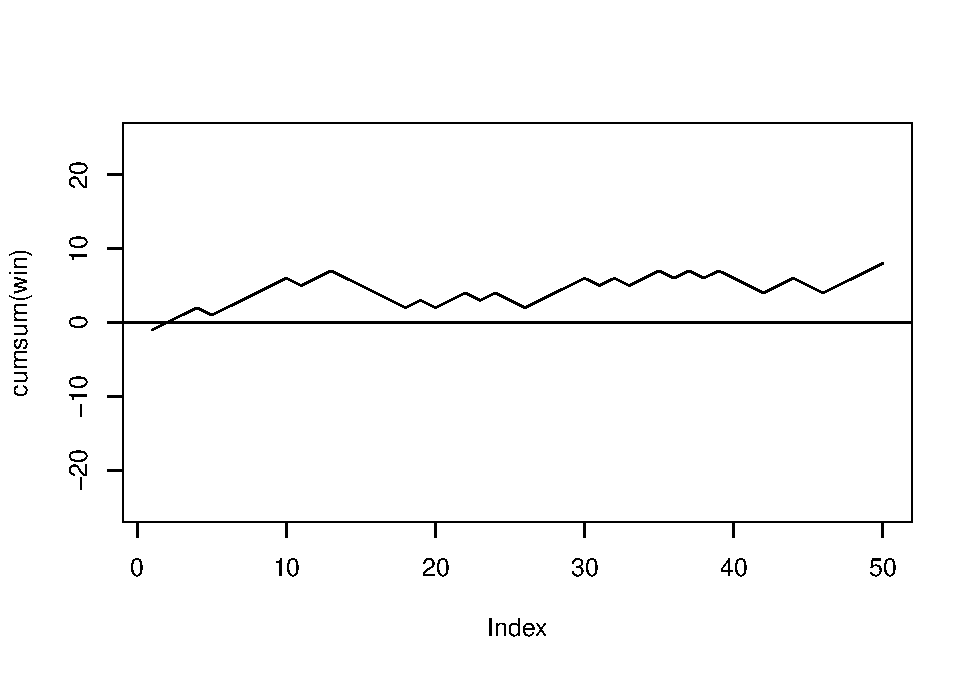
\includegraphics[width=0.5\linewidth]{SimBook_files/figure-latex/cumwin-1} 

}

\caption{Peter's fortune throughout one simulated game.}\label{fig:cumwin}
\end{figure}

Of course this is the result of a single simulation and the outcome may be totally different than the one we saw. Figure \ref{fig:mcumwin} reports four simulated games: we can see that in the first one Peter wins, in the second he almost breaks even, whilst in the third and fourth he clearly loses.

\begin{Shaded}
\begin{Highlighting}[]
\FunctionTok{set.seed}\NormalTok{(}\DecValTok{2021}\NormalTok{)}
\FunctionTok{par}\NormalTok{(}\AttributeTok{mfrow=}\FunctionTok{c}\NormalTok{(}\DecValTok{2}\NormalTok{, }\DecValTok{2}\NormalTok{))}
\ControlFlowTok{for}\NormalTok{(j }\ControlFlowTok{in} \DecValTok{1}\SpecialCharTok{:}\DecValTok{4}\NormalTok{)\{}
  \FunctionTok{plot}\NormalTok{(}\FunctionTok{cumsum}\NormalTok{(}\FunctionTok{sample}\NormalTok{(}\FunctionTok{c}\NormalTok{(}\SpecialCharTok{{-}}\DecValTok{1}\NormalTok{, }\DecValTok{1}\NormalTok{),}\AttributeTok{size=}\DecValTok{50}\NormalTok{,}\AttributeTok{replace=}\NormalTok{T)),}\AttributeTok{type=}\StringTok{"l"}\NormalTok{ ,}\AttributeTok{ylim=}\FunctionTok{c}\NormalTok{(}\SpecialCharTok{{-}}\DecValTok{25}\NormalTok{, }\DecValTok{25}\NormalTok{), }\AttributeTok{ylab=}\StringTok{"Outcome"}\NormalTok{)}
  \FunctionTok{abline}\NormalTok{(}\AttributeTok{h=}\DecValTok{0}\NormalTok{)\}}
\end{Highlighting}
\end{Shaded}

\begin{figure}

{\centering 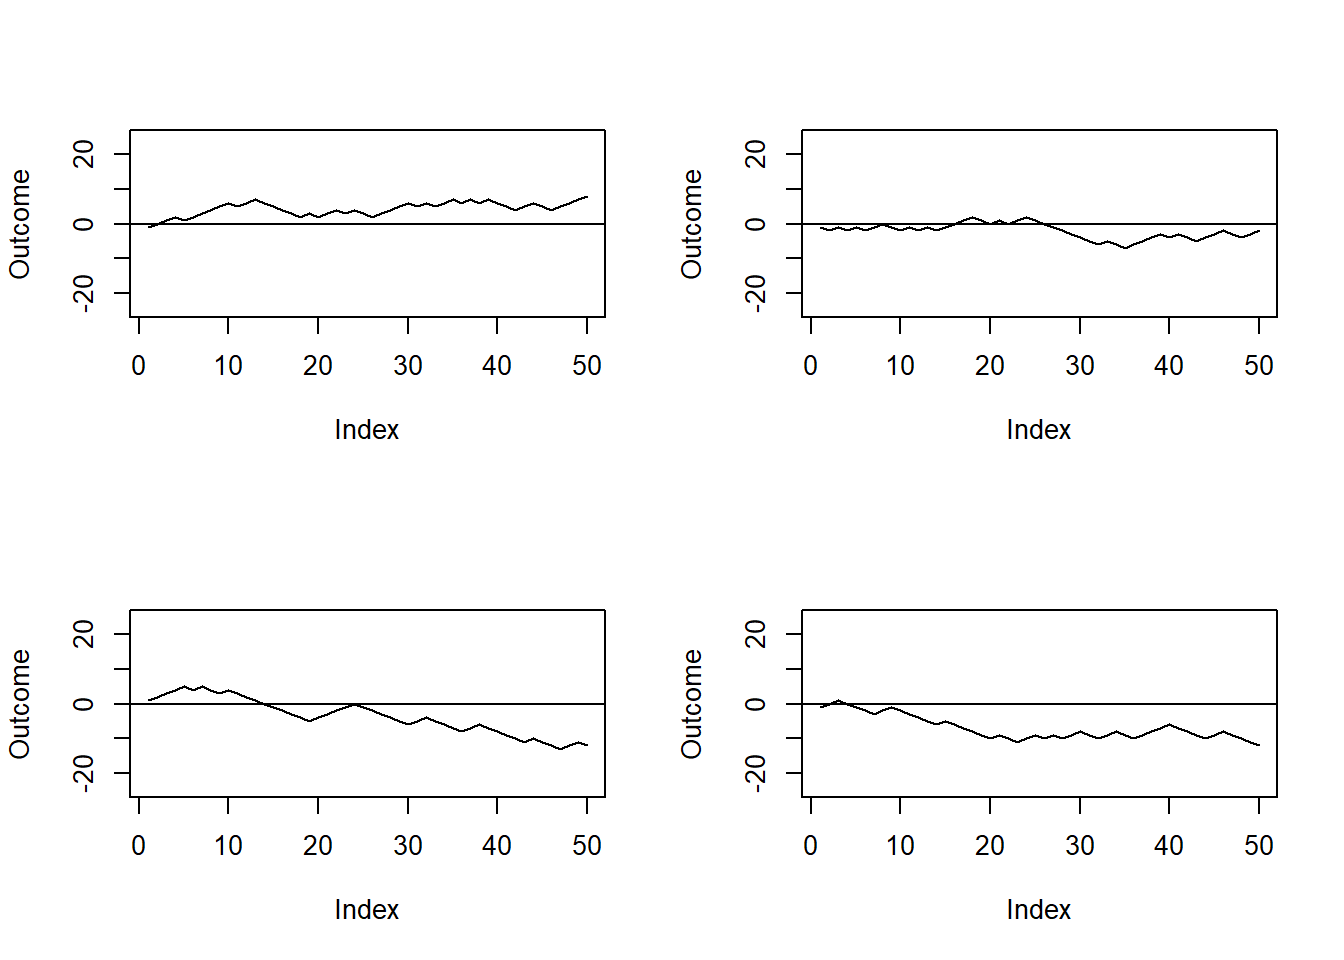
\includegraphics[width=0.8\linewidth]{SimBook_files/figure-latex/mcumwin-1} 

}

\caption{Outcome of four simulated game of chances.}\label{fig:mcumwin}
\end{figure}

Suppose we are interested in the following question.

\begin{itemize}
\tightlist
\item
  What is the probability that Peter breaks even at the end of the game?
\end{itemize}

Evidently we cannot cannot answer by simply looking at the outputs of the previous simulations. We need to do a formal Monte Carlo study. In this type of experiment, we simulate the random process and compute the statistic of interest. By repeating the random process many times, we obtain a collection of values of the statistic, which can then be used to approximate probabilities or expectations that answer the questions.

As you may recall from the estimation of \(\pi\) experiment, we first need to write a function that simulates the experiment. In particular we need to write a function which outputs Peter's winning at the end of the game. To make this function more general, we define \texttt{n} to be the number of tosses and let the default value of \texttt{n} be 50.

\begin{Shaded}
\begin{Highlighting}[]
\NormalTok{peter.paul }\OtherTok{\textless{}{-}} \ControlFlowTok{function}\NormalTok{(}\AttributeTok{n=}\DecValTok{50}\NormalTok{)\{}
  \FunctionTok{sum}\NormalTok{(}\FunctionTok{sample}\NormalTok{(}\FunctionTok{c}\NormalTok{(}\SpecialCharTok{{-}}\DecValTok{1}\NormalTok{, }\DecValTok{1}\NormalTok{), }\AttributeTok{size=}\NormalTok{n, }\AttributeTok{replace=}\ConstantTok{TRUE}\NormalTok{))}
\NormalTok{\}}
\FunctionTok{set.seed}\NormalTok{(}\DecValTok{2021}\NormalTok{)}
\FunctionTok{peter.paul}\NormalTok{()}
\end{Highlighting}
\end{Shaded}

\begin{verbatim}
## [1] 8
\end{verbatim}

The output is the same as the previous code, so it seems that our function works correctly.

Let's replicate the experiment many times.

\begin{Shaded}
\begin{Highlighting}[]
\FunctionTok{set.seed}\NormalTok{(}\DecValTok{2021}\NormalTok{)}
\NormalTok{experiment }\OtherTok{\textless{}{-}} \FunctionTok{replicate}\NormalTok{(}\DecValTok{1000}\NormalTok{,}\FunctionTok{peter.paul}\NormalTok{())}
\FunctionTok{head}\NormalTok{(experiment)}
\end{Highlighting}
\end{Shaded}

\begin{verbatim}
## [1]   8  -2 -12 -12 -14   8
\end{verbatim}

So the vector \texttt{experiment} stores Peter's final fortune in 1000 games. Since Peter's fortune is an integer-value variable, it is convenient to summarize it using the \texttt{table} function.

\begin{Shaded}
\begin{Highlighting}[]
\FunctionTok{table}\NormalTok{(experiment)}
\end{Highlighting}
\end{Shaded}

\begin{verbatim}
## experiment
## -22 -20 -18 -16 -14 -12 -10  -8  -6  -4  -2   0   2   4   6   8  10  12  14  16 
##   1   2   7   7  16  30  42  66  58 101 116 102 110 103  70  60  44  26  15  14 
##  18  20 
##   4   6
\end{verbatim}

A graphical representation of the table is also useful.

\begin{Shaded}
\begin{Highlighting}[]
\FunctionTok{plot}\NormalTok{(}\FunctionTok{table}\NormalTok{(experiment))}
\end{Highlighting}
\end{Shaded}

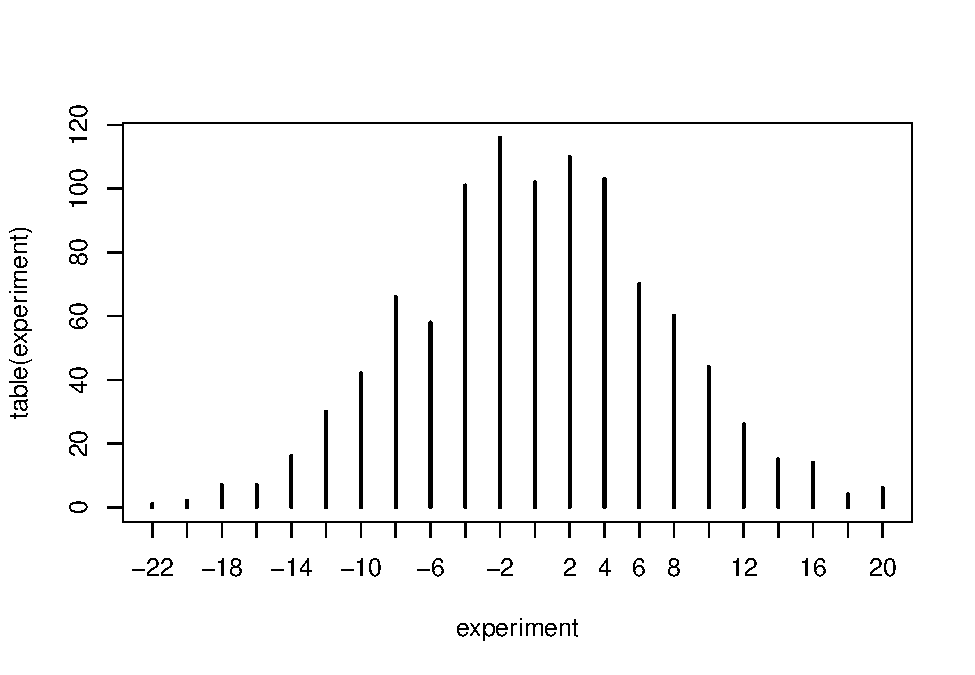
\includegraphics{SimBook_files/figure-latex/unnamed-chunk-113-1.pdf}
So we can see that Peter breaks even 102 out of 1000 times. Furthermore the plot shows us that most commonly Peter will win/lose little money and that big wins/losses are unlikely.

To conclude our experiment we need to calculate our estimated probability of Peter breaking even. Clearly this is equal to 102/1000= 0.102. In R:

\begin{Shaded}
\begin{Highlighting}[]
\FunctionTok{sum}\NormalTok{(experiment}\SpecialCharTok{==}\DecValTok{0}\NormalTok{)}\SpecialCharTok{/}\DecValTok{1000}
\end{Highlighting}
\end{Shaded}

\begin{verbatim}
## [1] 0.102
\end{verbatim}

Notice that we could have also answered this question exactly. The event Peter breaking even coincides with a number of successes \(n/2\) in a Binomial experiment with parameters \(n=50\) and \(\theta = 0.5\). This can be computed in R as

\begin{Shaded}
\begin{Highlighting}[]
\FunctionTok{dbinom}\NormalTok{(}\DecValTok{25}\NormalTok{, }\AttributeTok{size =} \DecValTok{50}\NormalTok{, }\AttributeTok{prob =} \FloatTok{0.5}\NormalTok{)}
\end{Highlighting}
\end{Shaded}

\begin{verbatim}
## [1] 0.1122752
\end{verbatim}

So our approximation is already quite close to the true value. We would get even closer by replicating the experiment a larger number of times.

\begin{Shaded}
\begin{Highlighting}[]
\FunctionTok{set.seed}\NormalTok{(}\DecValTok{2021}\NormalTok{)}
\NormalTok{experiment }\OtherTok{\textless{}{-}} \FunctionTok{replicate}\NormalTok{(}\DecValTok{10000}\NormalTok{,}\FunctionTok{peter.paul}\NormalTok{())}
\FunctionTok{length}\NormalTok{(experiment[experiment}\SpecialCharTok{==}\DecValTok{0}\NormalTok{])}\SpecialCharTok{/}\DecValTok{1000}
\end{Highlighting}
\end{Shaded}

\begin{verbatim}
## [1] 1.096
\end{verbatim}

\hypertarget{playing-the-roulette}{%
\section{Playing the roulette}\label{playing-the-roulette}}

Consider a European-style roulette which includes numbers between 0 and 36. In roulette there are many different betting alternatives but we consider here the simplest case where we bet on a single number. If we pick the right number then we win 35 times what we bet.

Consider the following scenario. We start playing roulette with a fixed \texttt{budget}. Every sping of the roulette costs one unit of \texttt{budget}. We play until we run out of budget and we always bet on the same number. The following function \texttt{roulette} implements this game.

\begin{Shaded}
\begin{Highlighting}[]
\NormalTok{roulette }\OtherTok{\textless{}{-}} \ControlFlowTok{function}\NormalTok{(budget, number)\{}
\NormalTok{  current }\OtherTok{\textless{}{-}} \FunctionTok{c}\NormalTok{()}
  \ControlFlowTok{while}\NormalTok{(budget }\SpecialCharTok{\textgreater{}} \DecValTok{0}\NormalTok{)\{}
\NormalTok{    outcome }\OtherTok{\textless{}{-}} \FunctionTok{sample}\NormalTok{(}\DecValTok{0}\SpecialCharTok{:}\DecValTok{36}\NormalTok{,}\DecValTok{1}\NormalTok{)}
    \ControlFlowTok{if}\NormalTok{(outcome }\SpecialCharTok{==}\NormalTok{ number) \{}
\NormalTok{      budget }\OtherTok{\textless{}{-}}\NormalTok{ budget }\SpecialCharTok{+} \DecValTok{35}
\NormalTok{    \}}
    \ControlFlowTok{else}\NormalTok{ \{budget }\OtherTok{\textless{}{-}}\NormalTok{ budget }\SpecialCharTok{{-}}\DecValTok{1}\NormalTok{\}}
\NormalTok{    current }\OtherTok{\textless{}{-}} \FunctionTok{c}\NormalTok{(current,budget)}
\NormalTok{  \}}
\NormalTok{  current}
\NormalTok{\}}
\end{Highlighting}
\end{Shaded}

It takes two inputs: the \texttt{budget} and the number we decided to play all the time. It outputs our budget throughout the whole game until it ends.

Let's play one game with a budget of 15 and betting on the number 8.

\begin{Shaded}
\begin{Highlighting}[]
\FunctionTok{set.seed}\NormalTok{(}\DecValTok{2021}\NormalTok{)}
\FunctionTok{roulette}\NormalTok{(}\DecValTok{15}\NormalTok{,}\DecValTok{8}\NormalTok{)}
\end{Highlighting}
\end{Shaded}

\begin{verbatim}
##  [1] 14 13 12 11 10  9  8  7  6  5  4  3  2  1  0
\end{verbatim}

In 15 spins the number 8 never comes up and therefore our game ends quite quickly.

We can ask ourselves many questions about such a game. For instance:

\begin{enumerate}
\def\labelenumi{\arabic{enumi}.}
\item
  What is the probability that the game last exactly 15 spins if I start with a budget of 15 and bet on the number 8?
\item
  What is the average length of the game starting with a budget of 15 and betting on the number 8?
\item
  What is the average maximum wealth I have during a game started with a budget of 15 and betting on the number 8?
\end{enumerate}

We will develop various Monte Carlo experiments to answer all the above questions. In each case, we simply need to modify the function \texttt{roulette} to output some summary about the game.

\hypertarget{question-1}{%
\subsection{Question 1}\label{question-1}}

\begin{enumerate}
\def\labelenumi{\arabic{enumi}.}
\tightlist
\item
  What is the probability that the game last exactly 15 spins if I start with a budget of 15 and bet on the number 8?
\end{enumerate}

If a game where I started with a budget of 15 ends after 15 spins, it means that the number 8 never showed up. We can adapt the function roulette to output \texttt{TRUE} if the length of the vector \texttt{wealth} is exactly equal to \texttt{budget}.

\begin{Shaded}
\begin{Highlighting}[]
\NormalTok{roulette1 }\OtherTok{\textless{}{-}} \ControlFlowTok{function}\NormalTok{(budget, number)\{}
\NormalTok{  wealth }\OtherTok{\textless{}{-}} \FunctionTok{c}\NormalTok{()}
\NormalTok{  current }\OtherTok{\textless{}{-}}\NormalTok{ budget}
  \ControlFlowTok{while}\NormalTok{(current }\SpecialCharTok{\textgreater{}} \DecValTok{0}\NormalTok{)\{}
\NormalTok{    outcome }\OtherTok{\textless{}{-}} \FunctionTok{sample}\NormalTok{(}\DecValTok{0}\SpecialCharTok{:}\DecValTok{36}\NormalTok{,}\DecValTok{1}\NormalTok{)}
    \ControlFlowTok{if}\NormalTok{(outcome }\SpecialCharTok{==}\NormalTok{ number) \{}
\NormalTok{      current }\OtherTok{\textless{}{-}}\NormalTok{ current }\SpecialCharTok{+} \DecValTok{35}
\NormalTok{    \}}
    \ControlFlowTok{else}\NormalTok{ \{current }\OtherTok{\textless{}{-}}\NormalTok{ current }\SpecialCharTok{{-}}\DecValTok{1}\NormalTok{\}}
\NormalTok{    wealth }\OtherTok{\textless{}{-}} \FunctionTok{c}\NormalTok{(wealth,current)}
\NormalTok{  \}}
  \ControlFlowTok{if}\NormalTok{(}\FunctionTok{length}\NormalTok{(wealth) }\SpecialCharTok{==}\NormalTok{ budget)\{}\FunctionTok{return}\NormalTok{(}\ConstantTok{TRUE}\NormalTok{)\} }\ControlFlowTok{else}\NormalTok{\{}\FunctionTok{return}\NormalTok{(}\ConstantTok{FALSE}\NormalTok{)\}}
\NormalTok{\}}
\end{Highlighting}
\end{Shaded}

Therefore for the previous example the function should output \texttt{TRUE}.

\begin{Shaded}
\begin{Highlighting}[]
\FunctionTok{set.seed}\NormalTok{(}\DecValTok{2021}\NormalTok{)}
\FunctionTok{roulette1}\NormalTok{(}\DecValTok{15}\NormalTok{,}\DecValTok{8}\NormalTok{)}
\end{Highlighting}
\end{Shaded}

\begin{verbatim}
## [1] TRUE
\end{verbatim}

Let's replicate the experiment 1000 times. The proportion of \texttt{TRUE} we observe is our estimate of this probability.

\begin{Shaded}
\begin{Highlighting}[]
\FunctionTok{set.seed}\NormalTok{(}\DecValTok{2021}\NormalTok{)}
\NormalTok{experiment }\OtherTok{\textless{}{-}} \FunctionTok{replicate}\NormalTok{(}\DecValTok{1000}\NormalTok{,}\FunctionTok{roulette1}\NormalTok{(}\DecValTok{15}\NormalTok{,}\DecValTok{8}\NormalTok{))}
\FunctionTok{sum}\NormalTok{(experiment)}\SpecialCharTok{/}\DecValTok{1000}
\end{Highlighting}
\end{Shaded}

\begin{verbatim}
## [1] 0.657
\end{verbatim}

Notice that actually we could have also computed this probability exactly. This is the probability that a Binomial random variable with parameter \(n=15\) (15 spins of the roulette) and \(\theta = 1/37\) (the number eight has probability 1/37 of appearing in a single spin) is equal to zero (no 8 can happen). This is equal to:

\begin{Shaded}
\begin{Highlighting}[]
\FunctionTok{dbinom}\NormalTok{(}\DecValTok{0}\NormalTok{,}\DecValTok{15}\NormalTok{,}\DecValTok{1}\SpecialCharTok{/}\DecValTok{37}\NormalTok{)}
\end{Highlighting}
\end{Shaded}

\begin{verbatim}
## [1] 0.6629971
\end{verbatim}

Therefore the Monte Carlo experiment approximates well the probability.

\hypertarget{question-2}{%
\subsection{Question 2}\label{question-2}}

\begin{enumerate}
\def\labelenumi{\arabic{enumi}.}
\setcounter{enumi}{1}
\tightlist
\item
  What is the average length of the game starting with a budget of 15 and betting on the number 8?
\end{enumerate}

We can answer this question by adapting the \texttt{roulette} function to output the length of the vector \texttt{wealth}.

\begin{Shaded}
\begin{Highlighting}[]
\NormalTok{roulette2 }\OtherTok{\textless{}{-}} \ControlFlowTok{function}\NormalTok{(budget, number)\{}
\NormalTok{  wealth }\OtherTok{\textless{}{-}} \FunctionTok{c}\NormalTok{()}
\NormalTok{  current }\OtherTok{\textless{}{-}}\NormalTok{ budget}
  \ControlFlowTok{while}\NormalTok{(current }\SpecialCharTok{\textgreater{}} \DecValTok{0}\NormalTok{)\{}
\NormalTok{    outcome }\OtherTok{\textless{}{-}} \FunctionTok{sample}\NormalTok{(}\DecValTok{0}\SpecialCharTok{:}\DecValTok{36}\NormalTok{,}\DecValTok{1}\NormalTok{)}
    \ControlFlowTok{if}\NormalTok{(outcome }\SpecialCharTok{==}\NormalTok{ number) \{}
\NormalTok{      current }\OtherTok{\textless{}{-}}\NormalTok{ current }\SpecialCharTok{+} \DecValTok{35}
\NormalTok{    \}}
    \ControlFlowTok{else}\NormalTok{ \{current }\OtherTok{\textless{}{-}}\NormalTok{ current }\SpecialCharTok{{-}}\DecValTok{1}\NormalTok{\}}
\NormalTok{    wealth }\OtherTok{\textless{}{-}} \FunctionTok{c}\NormalTok{(wealth,current)}
\NormalTok{  \}}
  \FunctionTok{length}\NormalTok{(wealth)}
\NormalTok{\}}
\end{Highlighting}
\end{Shaded}

In our example, the output should be 15.

\begin{Shaded}
\begin{Highlighting}[]
\FunctionTok{set.seed}\NormalTok{(}\DecValTok{2021}\NormalTok{)}
\FunctionTok{roulette2}\NormalTok{(}\DecValTok{15}\NormalTok{,}\DecValTok{8}\NormalTok{)}
\end{Highlighting}
\end{Shaded}

\begin{verbatim}
## [1] 15
\end{verbatim}

Let's replicate the experiment 1000 times and summarize the results with a plot (it may take some time to run the code!).

\begin{Shaded}
\begin{Highlighting}[]
\FunctionTok{set.seed}\NormalTok{(}\DecValTok{2021}\NormalTok{)}
\NormalTok{experiment }\OtherTok{\textless{}{-}} \FunctionTok{replicate}\NormalTok{(}\DecValTok{1000}\NormalTok{,}\FunctionTok{roulette2}\NormalTok{(}\DecValTok{15}\NormalTok{,}\DecValTok{8}\NormalTok{))}
\FunctionTok{plot}\NormalTok{(}\FunctionTok{table}\NormalTok{(experiment))}
\end{Highlighting}
\end{Shaded}

\begin{center}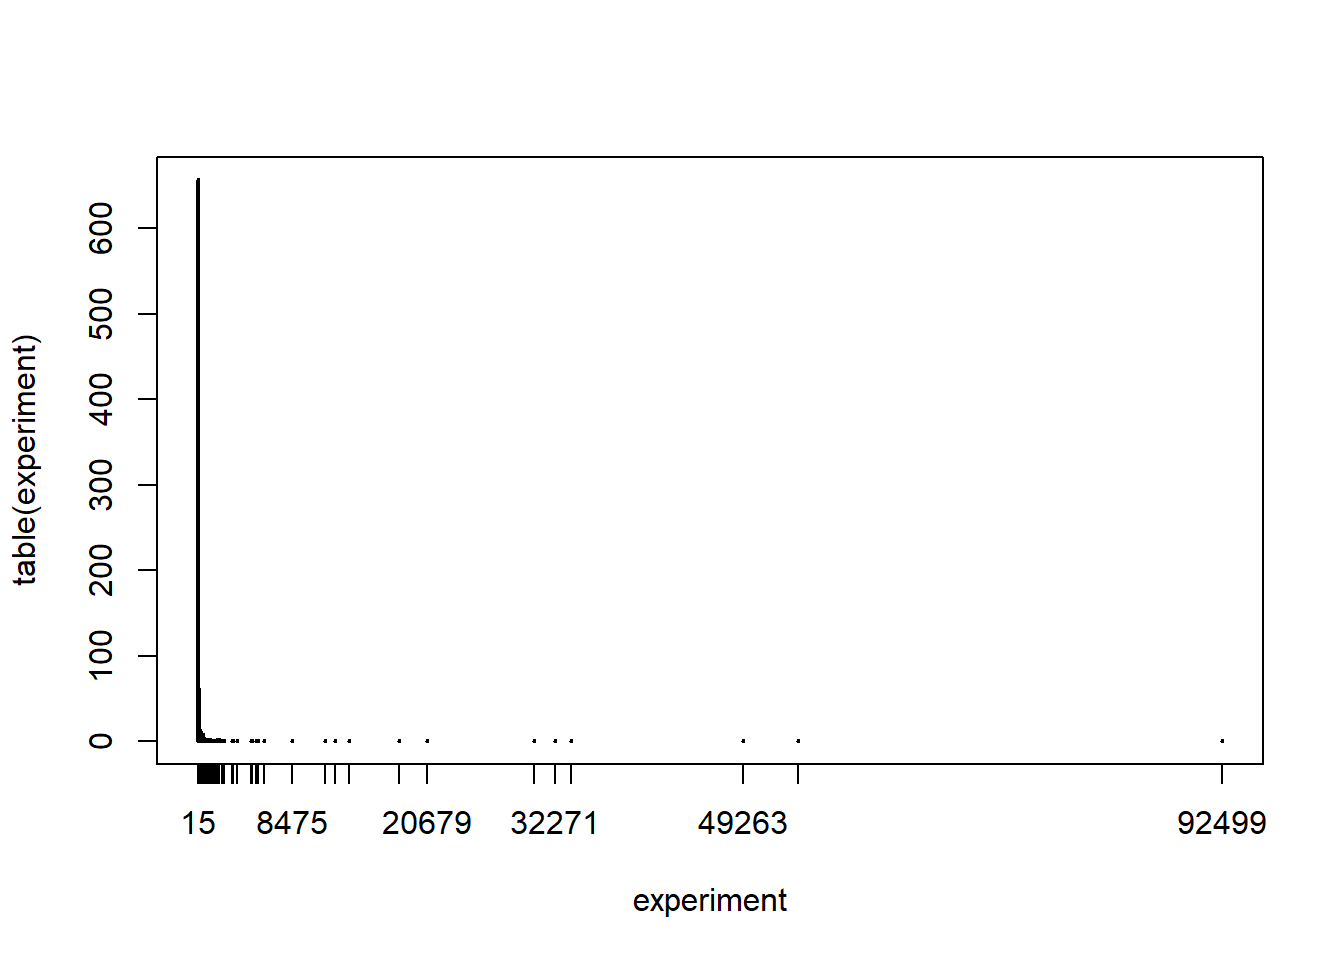
\includegraphics[width=0.5\linewidth]{SimBook_files/figure-latex/roulette2-1} \end{center}

We can see that the distribution is very skewed, most often the length is 15 spins, but then sometimes the game has a length which is much longer. Therefore, the median of the data is a much better option to summarize the average length of the game. We can compute it, together with a range of plausible values, as

\begin{Shaded}
\begin{Highlighting}[]
\FunctionTok{median}\NormalTok{(experiment)}
\end{Highlighting}
\end{Shaded}

\begin{verbatim}
## [1] 15
\end{verbatim}

\begin{Shaded}
\begin{Highlighting}[]
\FunctionTok{c}\NormalTok{(}\FunctionTok{sort}\NormalTok{(experiment)[}\DecValTok{25}\NormalTok{],}\FunctionTok{sort}\NormalTok{(experiment)[}\DecValTok{975}\NormalTok{])}
\end{Highlighting}
\end{Shaded}

\begin{verbatim}
## [1]   15 1923
\end{verbatim}

So we can see that the median is indeed 15: most of the times the number 8 does not appear and therefore the game ends in 15 spins.

\hypertarget{question-3}{%
\subsection{Question 3}\label{question-3}}

\begin{enumerate}
\def\labelenumi{\arabic{enumi}.}
\setcounter{enumi}{2}
\tightlist
\item
  What is the average maximum wealth I have during a game started with a budget of 15 and betting on the number 8?
\end{enumerate}

We can answer this question by adapting the \texttt{roulette} function to output the maximum of the vector \texttt{wealth}.

\begin{Shaded}
\begin{Highlighting}[]
\NormalTok{roulette3 }\OtherTok{\textless{}{-}} \ControlFlowTok{function}\NormalTok{(budget, number)\{}
\NormalTok{  wealth }\OtherTok{\textless{}{-}} \FunctionTok{c}\NormalTok{()}
\NormalTok{  current }\OtherTok{\textless{}{-}}\NormalTok{ budget}
  \ControlFlowTok{while}\NormalTok{(current }\SpecialCharTok{\textgreater{}} \DecValTok{0}\NormalTok{)\{}
\NormalTok{    outcome }\OtherTok{\textless{}{-}} \FunctionTok{sample}\NormalTok{(}\DecValTok{0}\SpecialCharTok{:}\DecValTok{36}\NormalTok{,}\DecValTok{1}\NormalTok{)}
    \ControlFlowTok{if}\NormalTok{(outcome }\SpecialCharTok{==}\NormalTok{ number) \{}
\NormalTok{      current }\OtherTok{\textless{}{-}}\NormalTok{ current }\SpecialCharTok{+} \DecValTok{35}
\NormalTok{    \}}
    \ControlFlowTok{else}\NormalTok{ \{current }\OtherTok{\textless{}{-}}\NormalTok{ current }\SpecialCharTok{{-}}\DecValTok{1}\NormalTok{\}}
\NormalTok{    wealth }\OtherTok{\textless{}{-}} \FunctionTok{c}\NormalTok{(wealth,current)}
\NormalTok{  \}}
  \FunctionTok{max}\NormalTok{(wealth)}
\NormalTok{\}}
\end{Highlighting}
\end{Shaded}

Let's again replicate the experiment and plot the result.

\begin{Shaded}
\begin{Highlighting}[]
\FunctionTok{set.seed}\NormalTok{(}\DecValTok{2021}\NormalTok{)}
\NormalTok{experiment }\OtherTok{\textless{}{-}} \FunctionTok{replicate}\NormalTok{(}\DecValTok{1000}\NormalTok{,}\FunctionTok{roulette3}\NormalTok{(}\DecValTok{15}\NormalTok{,}\DecValTok{8}\NormalTok{))}
\FunctionTok{plot}\NormalTok{(}\FunctionTok{table}\NormalTok{(experiment))}
\end{Highlighting}
\end{Shaded}

\begin{center}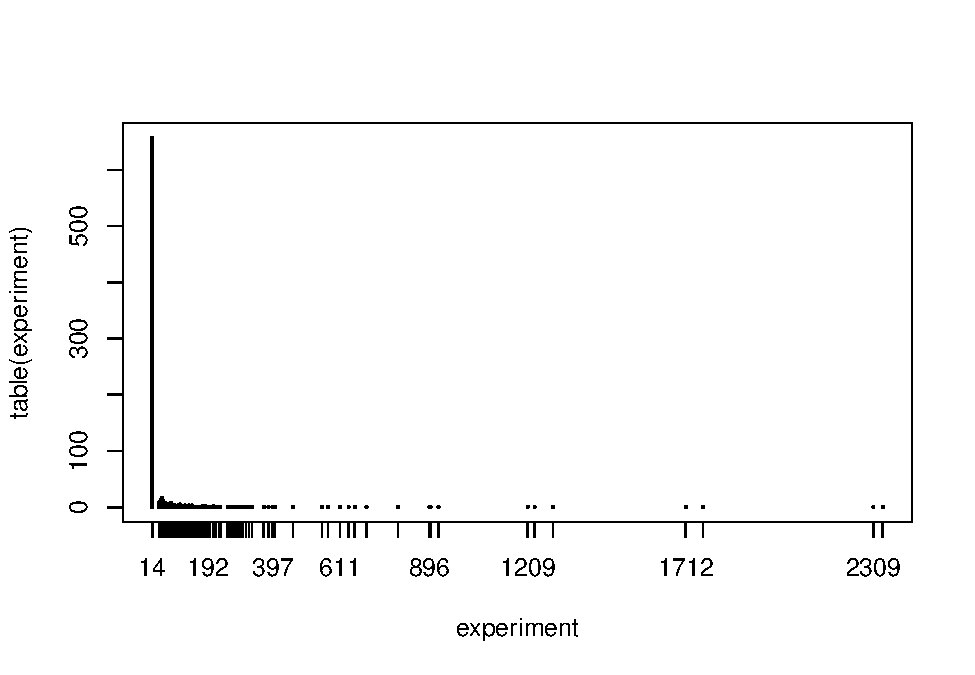
\includegraphics[width=0.5\linewidth]{SimBook_files/figure-latex/roulette3-1} \end{center}

We can then get an estimate of the maximum wealth as well as a range of plausible values as

\begin{Shaded}
\begin{Highlighting}[]
\FunctionTok{median}\NormalTok{(experiment)}
\end{Highlighting}
\end{Shaded}

\begin{verbatim}
## [1] 14
\end{verbatim}

\begin{Shaded}
\begin{Highlighting}[]
\FunctionTok{c}\NormalTok{(}\FunctionTok{sort}\NormalTok{(experiment)[}\DecValTok{25}\NormalTok{],}\FunctionTok{sort}\NormalTok{(experiment)[}\DecValTok{975}\NormalTok{])}
\end{Highlighting}
\end{Shaded}

\begin{verbatim}
## [1]  14 331
\end{verbatim}

Since most often the game ends with no 8 appearing, the maximum wealth is most often 14.

\hypertarget{is-annie-meeting-sam}{%
\section{Is Annie meeting Sam?}\label{is-annie-meeting-sam}}

Sleepless in Seattle is a 1993 American Romantic Comedy. Annie and Sam are supposed to meet on top of the Empire State Building where they would at last meet. However, their arrival time depends on a variety of factors and may actually not coincide and therefore never fall in love.

We make the following assumptions:

\begin{itemize}
\item
  Sam and Annie arrive independently;
\item
  Sam arrives between 10 pm and 11:30 pm uniformly;
\item
  Annie arrives between 10:30 pm and midnight uniformly.
\end{itemize}

We want to answer the following questions:

\begin{itemize}
\item
  What is the probability that Annie arrives before Sam?
\item
  What is the expected difference in arrival time?
\item
  If they each wait only twenty minutes after their arrival, what is the probability that they meet?
\item
  How much should they wait (assuming they wait the same amount of time), so that the probability they meet is at least 50\%?
\end{itemize}

\hypertarget{question-1-1}{%
\subsection{Question 1}\label{question-1-1}}

\begin{itemize}
\tightlist
\item
  What is the probability that Annie arrives before Sam?
\end{itemize}

The following function outputs \texttt{TRUE} if Annie arrives before Sam and \texttt{FALSE} otherwise.

\begin{Shaded}
\begin{Highlighting}[]
\NormalTok{sam\_annie1 }\OtherTok{\textless{}{-}} \ControlFlowTok{function}\NormalTok{()\{}
\NormalTok{  sam }\OtherTok{\textless{}{-}} \FunctionTok{runif}\NormalTok{(}\DecValTok{1}\NormalTok{,}\DecValTok{0}\NormalTok{,}\DecValTok{90}\NormalTok{)}
\NormalTok{  annie }\OtherTok{\textless{}{-}} \FunctionTok{runif}\NormalTok{(}\DecValTok{1}\NormalTok{,}\DecValTok{30}\NormalTok{,}\DecValTok{120}\NormalTok{)}
\NormalTok{  annie }\SpecialCharTok{\textless{}}\NormalTok{ sam}
\NormalTok{\}}
\end{Highlighting}
\end{Shaded}

If we run a single simulation for instance

\begin{Shaded}
\begin{Highlighting}[]
\FunctionTok{set.seed}\NormalTok{(}\DecValTok{2021}\NormalTok{)}
\FunctionTok{sam\_annie1}\NormalTok{()}
\end{Highlighting}
\end{Shaded}

\begin{verbatim}
## [1] FALSE
\end{verbatim}

We see that Annie does not arrive before Sam.

We can simply adapt \texttt{sam\_annie1} to use 1000 random observations and give an estimate of this probability.

\begin{Shaded}
\begin{Highlighting}[]
\NormalTok{sam\_annie1 }\OtherTok{\textless{}{-}} \ControlFlowTok{function}\NormalTok{()\{}
\NormalTok{  sam }\OtherTok{\textless{}{-}} \FunctionTok{runif}\NormalTok{(}\DecValTok{1000}\NormalTok{,}\DecValTok{0}\NormalTok{,}\DecValTok{90}\NormalTok{)}
\NormalTok{  annie }\OtherTok{\textless{}{-}} \FunctionTok{runif}\NormalTok{(}\DecValTok{1000}\NormalTok{,}\DecValTok{30}\NormalTok{,}\DecValTok{120}\NormalTok{)}
  \FunctionTok{sum}\NormalTok{(annie }\SpecialCharTok{\textless{}}\NormalTok{ sam)}\SpecialCharTok{/}\DecValTok{1000}
\NormalTok{\}}

\FunctionTok{set.seed}\NormalTok{(}\DecValTok{2021}\NormalTok{)}
\FunctionTok{sam\_annie1}\NormalTok{()}
\end{Highlighting}
\end{Shaded}

\begin{verbatim}
## [1] 0.223
\end{verbatim}

If we want to have an estimate of the variability around this probability we can then replicate the experiment.

\begin{Shaded}
\begin{Highlighting}[]
\FunctionTok{set.seed}\NormalTok{(}\DecValTok{2021}\NormalTok{)}
\NormalTok{experiment }\OtherTok{\textless{}{-}} \FunctionTok{replicate}\NormalTok{(}\DecValTok{1000}\NormalTok{, }\FunctionTok{sam\_annie1}\NormalTok{())}
\FunctionTok{boxplot}\NormalTok{(experiment)}
\end{Highlighting}
\end{Shaded}

\begin{center}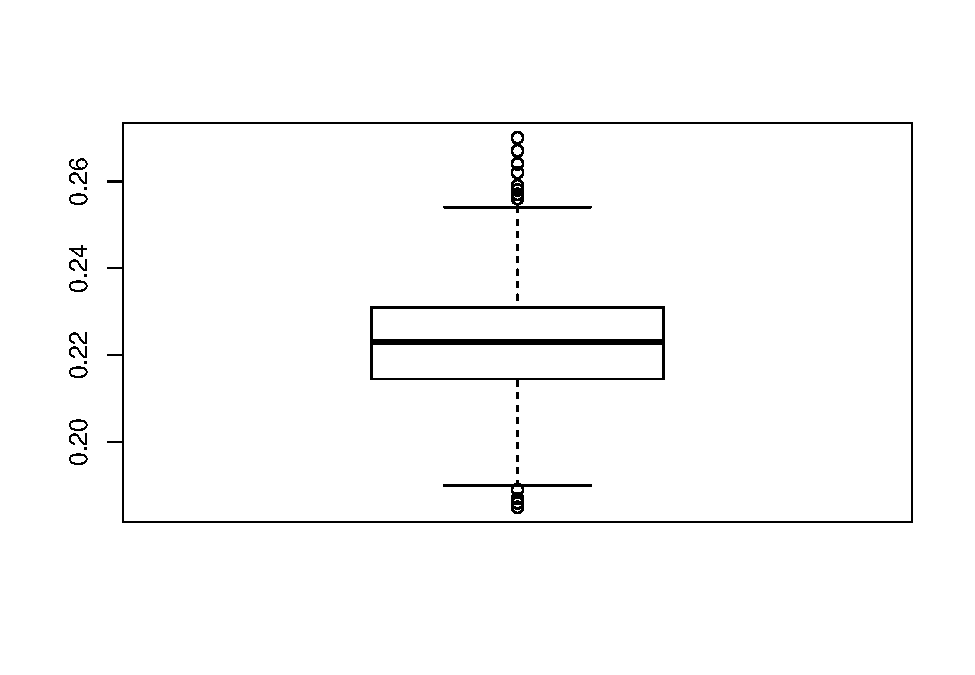
\includegraphics[width=0.5\linewidth]{SimBook_files/figure-latex/unnamed-chunk-131-1} \end{center}

The probability that Annie arrives before Sam is around 0.22.

\hypertarget{question-2-1}{%
\subsection{Question 2}\label{question-2-1}}

\begin{itemize}
\tightlist
\item
  What is the expected difference in arrival time?
\end{itemize}

The function \texttt{sam\_annie2} computes this expectation using 1000 random observations.

\begin{Shaded}
\begin{Highlighting}[]
\NormalTok{sam\_annie2 }\OtherTok{\textless{}{-}} \ControlFlowTok{function}\NormalTok{()\{}
\NormalTok{  sam }\OtherTok{\textless{}{-}} \FunctionTok{runif}\NormalTok{(}\DecValTok{1000}\NormalTok{,}\DecValTok{0}\NormalTok{,}\DecValTok{90}\NormalTok{)}
\NormalTok{  annie }\OtherTok{\textless{}{-}} \FunctionTok{runif}\NormalTok{(}\DecValTok{1000}\NormalTok{,}\DecValTok{30}\NormalTok{,}\DecValTok{120}\NormalTok{)}
  \FunctionTok{mean}\NormalTok{(sam}\SpecialCharTok{{-}}\NormalTok{annie)}
\NormalTok{\}}
\end{Highlighting}
\end{Shaded}

We can replicate and create a boxplot.

\begin{Shaded}
\begin{Highlighting}[]
\FunctionTok{set.seed}\NormalTok{(}\DecValTok{2021}\NormalTok{)}
\NormalTok{experiment }\OtherTok{\textless{}{-}} \FunctionTok{replicate}\NormalTok{(}\DecValTok{1000}\NormalTok{,}\FunctionTok{sam\_annie2}\NormalTok{())}
\FunctionTok{boxplot}\NormalTok{(experiment)}
\end{Highlighting}
\end{Shaded}

\begin{center}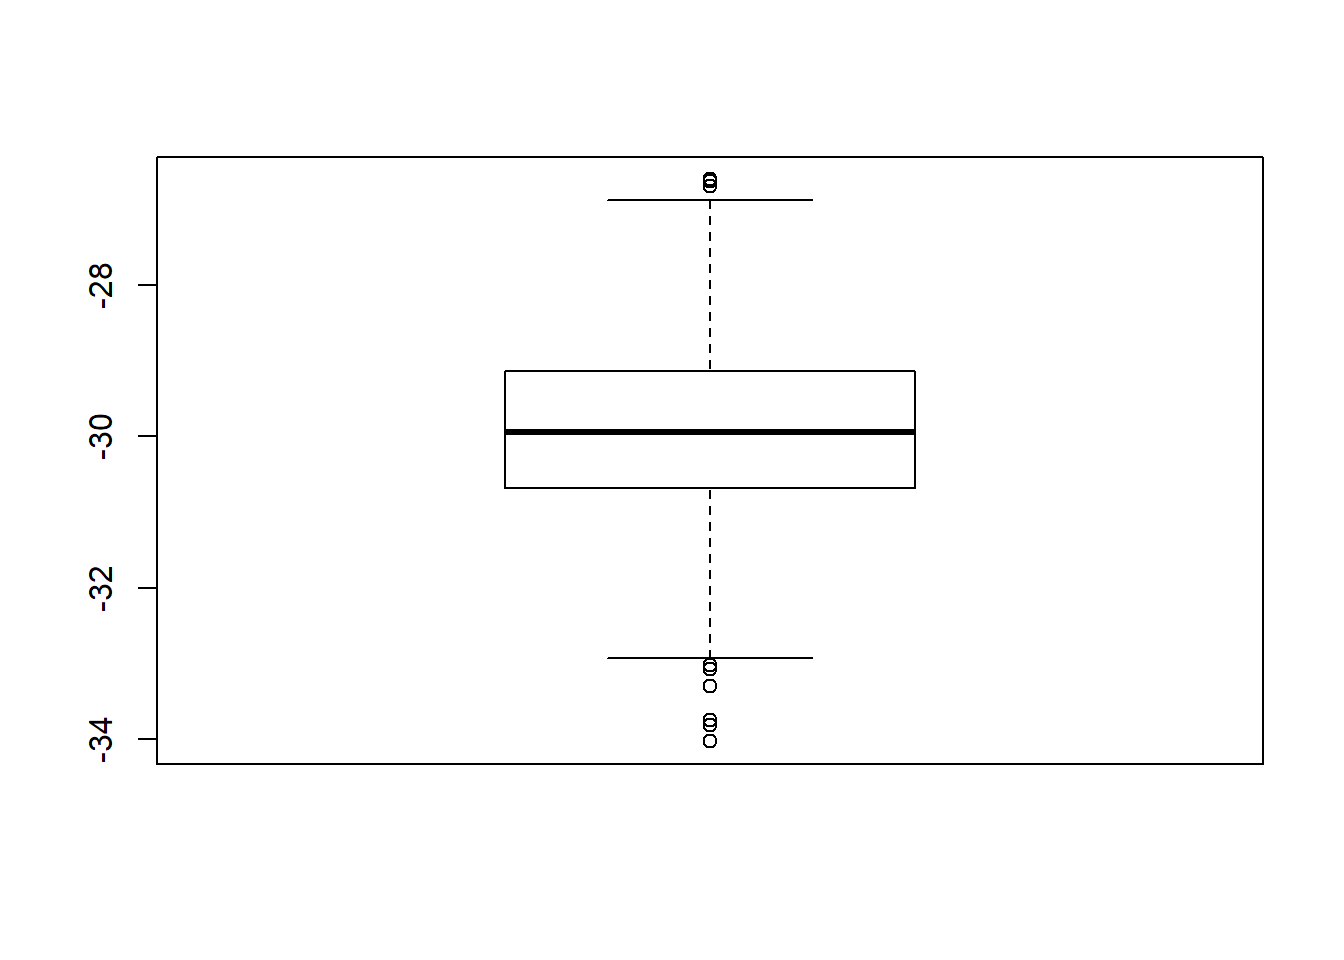
\includegraphics[width=0.5\linewidth]{SimBook_files/figure-latex/unnamed-chunk-133-1} \end{center}

So on average Sam arrives 30 minutes before Annie.

\hypertarget{question-3-1}{%
\subsection{Question 3}\label{question-3-1}}

\begin{itemize}
\tightlist
\item
  If they each wait only twenty minutes after their arrival, what is the probability that they meet?
\end{itemize}

The function \texttt{sleepless} below returns \texttt{TRUE} if Annie and Sam meets,\texttt{FALSE} otherwise.

\begin{Shaded}
\begin{Highlighting}[]
\NormalTok{sleepless }\OtherTok{\textless{}{-}} \ControlFlowTok{function}\NormalTok{(}\AttributeTok{waiting =} \DecValTok{20}\NormalTok{)\{}
\NormalTok{  u1 }\OtherTok{\textless{}{-}} \FunctionTok{runif}\NormalTok{(}\DecValTok{1}\NormalTok{,}\DecValTok{0}\NormalTok{,}\DecValTok{150}\NormalTok{)}
\NormalTok{  u2 }\OtherTok{\textless{}{-}} \FunctionTok{runif}\NormalTok{(}\DecValTok{1}\NormalTok{,}\DecValTok{50}\NormalTok{,}\DecValTok{200}\NormalTok{)}
  \ControlFlowTok{if}\NormalTok{ (u1 }\SpecialCharTok{\textless{}}\NormalTok{ u2)\{}\ControlFlowTok{if}\NormalTok{(u1 }\SpecialCharTok{+}\NormalTok{ waiting }\SpecialCharTok{\textgreater{}}\NormalTok{ u2) }\FunctionTok{return}\NormalTok{(}\ConstantTok{TRUE}\NormalTok{)\}}
  \ControlFlowTok{else}\NormalTok{\{}\ControlFlowTok{if}\NormalTok{ (u2 }\SpecialCharTok{+}\NormalTok{ waiting }\SpecialCharTok{\textgreater{}}\NormalTok{ u1) }\FunctionTok{return}\NormalTok{(}\ConstantTok{TRUE}\NormalTok{)\}}
  \FunctionTok{return}\NormalTok{(}\ConstantTok{FALSE}\NormalTok{)}
\NormalTok{\}}
\end{Highlighting}
\end{Shaded}

Let's run it 10.000 times to get an estimate of the probability.

\begin{Shaded}
\begin{Highlighting}[]
\FunctionTok{set.seed}\NormalTok{(}\DecValTok{2021}\NormalTok{)}
\FunctionTok{mean}\NormalTok{(}\FunctionTok{replicate}\NormalTok{(}\DecValTok{10000}\NormalTok{,}\FunctionTok{sleepless}\NormalTok{()))}
\end{Highlighting}
\end{Shaded}

\begin{verbatim}
## [1] 0.178
\end{verbatim}

So we see that if they each wait 20 minutes, they have a probability of meeting of 0.178.

\hypertarget{question-4}{%
\subsection{Question 4}\label{question-4}}

\begin{itemize}
\tightlist
\item
  How much should they wait (assuming they wait the same amount of time), so that the probability they meet is at least 50\%?
\end{itemize}

In order to answer this question we can use the \texttt{sapply} function. We already know that if they wait 20 minutes, the probability of meeting is 0.19. So we consider longer waiting times.

\begin{Shaded}
\begin{Highlighting}[]
\FunctionTok{sapply}\NormalTok{(}\DecValTok{30}\SpecialCharTok{:}\DecValTok{60}\NormalTok{,}\ControlFlowTok{function}\NormalTok{(x) }\FunctionTok{mean}\NormalTok{(}\FunctionTok{replicate}\NormalTok{(}\DecValTok{10000}\NormalTok{,}\FunctionTok{sleepless}\NormalTok{(x))))}
\end{Highlighting}
\end{Shaded}

\begin{verbatim}
##  [1] 0.2754 0.2769 0.2811 0.2925 0.3055 0.3104 0.3147 0.3248 0.3400 0.3482
## [11] 0.3571 0.3605 0.3746 0.3869 0.3958 0.4034 0.4104 0.4184 0.4237 0.4283
## [21] 0.4444 0.4653 0.4664 0.4763 0.4831 0.4846 0.4929 0.5067 0.5091 0.5222
## [31] 0.5312
\end{verbatim}

It's the 28th entry of the vector \texttt{30:60}, that is 57, the first one for which the probability is at least 0.50. So they should wait 57 minutes if they want to have a probability of at least 50\% to actually meet.

\hypertarget{discrete-event-simulation}{%
\chapter{Discrete Event Simulation}\label{discrete-event-simulation}}

The complexity of many real-world systems involves unaffordable analytical models, and consequently, such systems are commonly studied by means of simulation. Different types of simulation apply depending on the nature of the system under consideration. In the last chapter we focused on static simulation, also called Monte Carlo simulation. In this chapter we discuss discrete-event simulation (DES) which is a specific technique for modelling stochastic, dynamic and discretely evolving systems. As opposed to continuous simulation, which typically uses smoothly-evolving equational models, DES is characterized by sudden state changes at precise points of (simulated) time.

Customers arriving at a bank, products being manipulated in a supply chain, or packets traversing a network are common examples of such systems. The discrete nature of a given system arises as soon as its behavior can be described in terms of events, which is the most fundamental concept in DES. An event is an instantaneous occurrence that may change the state of the system, while, between events, all the state variables remain constant.

To implement DES in R we will take advantage of the \texttt{simmer} package which provides capabilities to easily model a wide range of applications.

\hypertarget{the-donut-shop}{%
\section{The donut shop}\label{the-donut-shop}}

You may recall that in Chapter 1 we discussed the example of a simple donut shop where we were interested in the waiting time of costumers depending on the number of employees in the shop. We will slowly build a more and more realistic implementation of the shop using \texttt{simmer}. First, if you have never done this, you need to install the package using the code

\begin{Shaded}
\begin{Highlighting}[]
\FunctionTok{install.packages}\NormalTok{(}\StringTok{"simmer"}\NormalTok{)}
\end{Highlighting}
\end{Shaded}

Once it is installed (that you only need to do once), you then need to load it at the beginning of every R session using the code

\begin{Shaded}
\begin{Highlighting}[]
\FunctionTok{library}\NormalTok{(simmer)}
\end{Highlighting}
\end{Shaded}

As we will see \texttt{simmer} takes advantage of the \texttt{magrittr} pipe operator.

\hypertarget{a-single-customer-at-a-fixed-time}{%
\subsection{A single customer at a fixed time}\label{a-single-customer-at-a-fixed-time}}

We first model a single customer who arrives at the shop for a visit, looks around at the decor for a time and then leaves. There is no queueing. First we will assume his arrival time and the time he spends in the shop are fixed.

The arrival time is fixed at 5, and the time spent in the shop is fixed at 10. We interpret `5' and `10' as `5 minutes' and `10 minutes'. The simulation runs for a maximum of 100 minutes, or until all the customers that are generated complete their visit to the shop.

Let's define step by step the code that implements this. First we define a variable called \texttt{customer} which describes the evolution of the customer in the shop. The evolution of the customer is called the \texttt{trajectory} and it is given some name. The function \texttt{log\_} produces text which is shown as specific points during the simulation. Lastly, \texttt{timeout} specifies how long the customer will spend in the shop.

\begin{Shaded}
\begin{Highlighting}[]
\NormalTok{customer }\OtherTok{\textless{}{-}}
  \FunctionTok{trajectory}\NormalTok{(}\StringTok{"Customer\textquotesingle{}s path"}\NormalTok{) }\SpecialCharTok{\%\textgreater{}\%}
  \FunctionTok{log\_}\NormalTok{(}\StringTok{"Here I am"}\NormalTok{) }\SpecialCharTok{\%\textgreater{}\%}
  \FunctionTok{timeout}\NormalTok{(}\DecValTok{10}\NormalTok{) }\SpecialCharTok{\%\textgreater{}\%}
  \FunctionTok{log\_}\NormalTok{(}\StringTok{"I must leave"}\NormalTok{)}
\end{Highlighting}
\end{Shaded}

Now that we have described how the customer behaves in the shop, we must create a variable specifying how the shop itself works. The code below creates the variable \texttt{shop} where first we create a \texttt{simmer} object called \texttt{shop} and then we specify via the function \texttt{add\_generator} that a customer arrives after 5 minutes.

\begin{Shaded}
\begin{Highlighting}[]
\NormalTok{shop }\OtherTok{\textless{}{-}}
  \FunctionTok{simmer}\NormalTok{(}\StringTok{"shop"}\NormalTok{) }\SpecialCharTok{\%\textgreater{}\%}
  \FunctionTok{add\_generator}\NormalTok{(}\StringTok{"Customer"}\NormalTok{, customer, }\FunctionTok{at}\NormalTok{(}\DecValTok{5}\NormalTok{))}
\end{Highlighting}
\end{Shaded}

Now that the shop is created we have to run the simulation using the \texttt{run} command.

\begin{Shaded}
\begin{Highlighting}[]
\NormalTok{shop }\SpecialCharTok{\%\textgreater{}\%} \FunctionTok{run}\NormalTok{(}\AttributeTok{until =} \DecValTok{100}\NormalTok{)}
\end{Highlighting}
\end{Shaded}

\begin{verbatim}
## 5: Customer0: Here I am
## 15: Customer0: I must leave
\end{verbatim}

\begin{verbatim}
## simmer environment: shop | now: 15 | next: 
## { Monitor: in memory }
## { Source: Customer | monitored: 1 | n_generated: 1 }
\end{verbatim}

The output summarizes what happened during the simulation. A customer arrives at minute 5 and leaves at minute 15. The simulation then stops since there are no other events that can happen in this simple case.

In order to have an overview of the events of the simulation we can also use the function \texttt{get\_mon\_arrivals}.

\begin{Shaded}
\begin{Highlighting}[]
\NormalTok{shop }\SpecialCharTok{\%\textgreater{}\%} \FunctionTok{get\_mon\_arrivals}\NormalTok{()}
\end{Highlighting}
\end{Shaded}

\begin{verbatim}
##        name start_time end_time activity_time finished replication
## 1 Customer0          5       15            10     TRUE           1
\end{verbatim}

\hypertarget{a-customer-arriving-at-random}{%
\subsection{A customer arriving at random}\label{a-customer-arriving-at-random}}

Now we extend the model to allow our customer to arrive at a random simulated time though we will keep the time in the bank at 10, as before.

The change occurs in the arguments to the \texttt{add\_generator} function. We will assume that the customer arrival time is generated from an Exponential distribution with parameter 1/5 (that is mean = 5).

\begin{Shaded}
\begin{Highlighting}[]
\FunctionTok{set.seed}\NormalTok{(}\DecValTok{2021}\NormalTok{)}

\NormalTok{customer }\OtherTok{\textless{}{-}}
  \FunctionTok{trajectory}\NormalTok{(}\StringTok{"Customer\textquotesingle{}s path"}\NormalTok{) }\SpecialCharTok{\%\textgreater{}\%}
  \FunctionTok{log\_}\NormalTok{(}\StringTok{"Here I am"}\NormalTok{) }\SpecialCharTok{\%\textgreater{}\%}
  \FunctionTok{timeout}\NormalTok{(}\DecValTok{10}\NormalTok{) }\SpecialCharTok{\%\textgreater{}\%}
  \FunctionTok{log\_}\NormalTok{(}\StringTok{"I must leave"}\NormalTok{)}

\NormalTok{shop }\OtherTok{\textless{}{-}}
  \FunctionTok{simmer}\NormalTok{(}\StringTok{"shop"}\NormalTok{) }\SpecialCharTok{\%\textgreater{}\%}
  \FunctionTok{add\_generator}\NormalTok{(}\StringTok{"Customer"}\NormalTok{, customer, }\FunctionTok{at}\NormalTok{(}\FunctionTok{rexp}\NormalTok{(}\DecValTok{1}\NormalTok{, }\DecValTok{1}\SpecialCharTok{/}\DecValTok{5}\NormalTok{)))}

\NormalTok{shop }\SpecialCharTok{\%\textgreater{}\%} \FunctionTok{run}\NormalTok{(}\AttributeTok{until =} \DecValTok{100}\NormalTok{)}
\end{Highlighting}
\end{Shaded}

\begin{verbatim}
## 5.92531: Customer0: Here I am
## 15.9253: Customer0: I must leave
\end{verbatim}

\begin{verbatim}
## simmer environment: shop | now: 15.925307087372 | next: 
## { Monitor: in memory }
## { Source: Customer | monitored: 1 | n_generated: 1 }
\end{verbatim}

\begin{Shaded}
\begin{Highlighting}[]
\NormalTok{shop }\SpecialCharTok{\%\textgreater{}\%} \FunctionTok{get\_mon\_arrivals}\NormalTok{()}
\end{Highlighting}
\end{Shaded}

\begin{verbatim}
##        name start_time end_time activity_time finished replication
## 1 Customer0   5.925307 15.92531            10     TRUE           1
\end{verbatim}

The trace shows that the customer now arrives at time 5.925307. Changing the seed value would change that time.

\hypertarget{many-random-customers}{%
\subsection{Many random customers}\label{many-random-customers}}

We now extend this model to allow multiple arrivals at random. In simulation this is usually interpreted as meaning that the times between customer arrivals are distributed as exponential random variables (we will see later on why this is so). There is little change in our program: we need to adapt the \texttt{add\_generator} function. We will run the simulation a shorter time, since otherwise the output becomes massive.

\begin{Shaded}
\begin{Highlighting}[]
\FunctionTok{set.seed}\NormalTok{(}\DecValTok{2021}\NormalTok{)}

\NormalTok{customer }\OtherTok{\textless{}{-}}
  \FunctionTok{trajectory}\NormalTok{(}\StringTok{"Customer\textquotesingle{}s path"}\NormalTok{) }\SpecialCharTok{\%\textgreater{}\%}
  \FunctionTok{log\_}\NormalTok{(}\StringTok{"Here I am"}\NormalTok{) }\SpecialCharTok{\%\textgreater{}\%}
  \FunctionTok{timeout}\NormalTok{(}\DecValTok{10}\NormalTok{) }\SpecialCharTok{\%\textgreater{}\%}
  \FunctionTok{log\_}\NormalTok{(}\StringTok{"I must leave"}\NormalTok{)}

\NormalTok{shop }\OtherTok{\textless{}{-}}
  \FunctionTok{simmer}\NormalTok{(}\StringTok{"shop"}\NormalTok{) }\SpecialCharTok{\%\textgreater{}\%}
  \FunctionTok{add\_generator}\NormalTok{(}\StringTok{"Customer"}\NormalTok{, customer, }\ControlFlowTok{function}\NormalTok{() }\FunctionTok{rexp}\NormalTok{(}\DecValTok{1}\NormalTok{, }\DecValTok{1}\SpecialCharTok{/}\DecValTok{5}\NormalTok{))}

\NormalTok{shop }\SpecialCharTok{\%\textgreater{}\%} \FunctionTok{run}\NormalTok{(}\AttributeTok{until =} \DecValTok{30}\NormalTok{)}
\end{Highlighting}
\end{Shaded}

\begin{verbatim}
## 5.92531: Customer0: Here I am
## 12.0259: Customer1: Here I am
## 13.3892: Customer2: Here I am
## 15.4026: Customer3: Here I am
## 15.9253: Customer0: I must leave
## 16.807: Customer4: Here I am
## 20.6063: Customer5: Here I am
## 22.0259: Customer1: I must leave
## 23.3892: Customer2: I must leave
## 23.7606: Customer6: Here I am
## 23.8551: Customer7: Here I am
## 24.5296: Customer8: Here I am
## 25.4026: Customer3: I must leave
## 26.807: Customer4: I must leave
## 27.7301: Customer9: Here I am
\end{verbatim}

\begin{verbatim}
## simmer environment: shop | now: 30 | next: 30.6063456850162
## { Monitor: in memory }
## { Source: Customer | monitored: 1 | n_generated: 11 }
\end{verbatim}

\begin{Shaded}
\begin{Highlighting}[]
\NormalTok{shop }\SpecialCharTok{\%\textgreater{}\%} \FunctionTok{get\_mon\_arrivals}\NormalTok{()}
\end{Highlighting}
\end{Shaded}

\begin{verbatim}
##        name start_time end_time activity_time finished replication
## 1 Customer0   5.925307 15.92531            10     TRUE           1
## 2 Customer1  12.025928 22.02593            10     TRUE           1
## 3 Customer2  13.389166 23.38917            10     TRUE           1
## 4 Customer3  15.402626 25.40263            10     TRUE           1
## 5 Customer4  16.807015 26.80702            10     TRUE           1
\end{verbatim}

So we see that in the 30 minutes we simulated, 10 customers arrived at the shop and 5 of them left after staying there for 10 minutes.

\hypertarget{the-donut-shop-with-a-service-counter}{%
\subsection{The donut shop with a service counter}\label{the-donut-shop-with-a-service-counter}}

So far, the model has been more like an art gallery, the customers entering, looking around, and leaving. Now they are going to require service from an employee. We extend the model to include a service counter that will be modelled as a `resource'. The actions of a Resource are simple: a customer requests a unit of the resource (an employee). If one is free, then the customer gets service (and the unit is no longer available to other customers). If there is no free employee, then the customer joins the queue until it is the customer's turn to be served. As each customer completes service and releases the unit, the employee can start serving the next in line.

The service counter is created with the \texttt{add\_resource} function. Default arguments specify that it can serve one customer at a time, and has infinite queuing capacity.

The \texttt{seize} function causes the customer to join the queue at the counter. If the queue is empty and the counter is available (not serving any customers), then the customer claims the counter for itself and moves onto the \texttt{timeout} step. Otherwise the customer must wait until the counter becomes available. Behaviour of the customer while in the queue is controlled by the arguments of the \texttt{seize} function. Once the \texttt{timeout} step is complete, the \texttt{release} function causes the customer to make the counter available to other customers in the queue.

We will assume that serving time follows a Normal distribution with mean 10 and standard deviation 2.

\begin{Shaded}
\begin{Highlighting}[]
\FunctionTok{set.seed}\NormalTok{(}\DecValTok{2021}\NormalTok{)}

\NormalTok{customer }\OtherTok{\textless{}{-}}
  \FunctionTok{trajectory}\NormalTok{(}\StringTok{"Customer\textquotesingle{}s path"}\NormalTok{) }\SpecialCharTok{\%\textgreater{}\%}
  \FunctionTok{log\_}\NormalTok{(}\StringTok{"Here I am"}\NormalTok{) }\SpecialCharTok{\%\textgreater{}\%}
  \FunctionTok{seize}\NormalTok{(}\StringTok{"counter"}\NormalTok{) }\SpecialCharTok{\%\textgreater{}\%}
  \FunctionTok{timeout}\NormalTok{(}\ControlFlowTok{function}\NormalTok{() }\FunctionTok{rnorm}\NormalTok{(}\DecValTok{1}\NormalTok{,}\DecValTok{10}\NormalTok{,}\DecValTok{2}\NormalTok{)) }\SpecialCharTok{\%\textgreater{}\%}
  \FunctionTok{release}\NormalTok{(}\StringTok{"counter"}\NormalTok{) }\SpecialCharTok{\%\textgreater{}\%}
  \FunctionTok{log\_}\NormalTok{(}\StringTok{"Finished"}\NormalTok{)}

\NormalTok{shop }\OtherTok{\textless{}{-}}
  \FunctionTok{simmer}\NormalTok{(}\StringTok{"shop"}\NormalTok{) }\SpecialCharTok{\%\textgreater{}\%}
  \FunctionTok{add\_resource}\NormalTok{(}\StringTok{"counter"}\NormalTok{) }\SpecialCharTok{\%\textgreater{}\%}
  \FunctionTok{add\_generator}\NormalTok{(}\StringTok{"Customer"}\NormalTok{, customer, }\ControlFlowTok{function}\NormalTok{() }\FunctionTok{rexp}\NormalTok{(}\DecValTok{1}\NormalTok{, }\DecValTok{1}\SpecialCharTok{/}\DecValTok{5}\NormalTok{))}

\NormalTok{shop }\SpecialCharTok{\%\textgreater{}\%} \FunctionTok{run}\NormalTok{(}\AttributeTok{until =} \DecValTok{30}\NormalTok{)}
\end{Highlighting}
\end{Shaded}

\begin{verbatim}
## 5.92531: Customer0: Here I am
## 12.0259: Customer1: Here I am
## 13.4303: Customer2: Here I am
## 16.6226: Customer0: Finished
## 17.2296: Customer3: Here I am
## 28.4187: Customer1: Finished
\end{verbatim}

\begin{verbatim}
## simmer environment: shop | now: 30 | next: 36.6490003143151
## { Monitor: in memory }
## { Resource: counter | monitored: TRUE | server status: 1(1) | queue status: 1(Inf) }
## { Source: Customer | monitored: 1 | n_generated: 5 }
\end{verbatim}

So we see that 4 customers arrived in the shop and that 2 of them were served. Let's use the function \texttt{get\_mon\_arrivals} to have a summary of each customer. By default, the function does not tell us the waiting time for a customer, which we will need to compute.

\begin{Shaded}
\begin{Highlighting}[]
\NormalTok{shop }\SpecialCharTok{\%\textgreater{}\%}
  \FunctionTok{get\_mon\_arrivals}\NormalTok{() }\SpecialCharTok{\%\textgreater{}\%}
  \FunctionTok{transform}\NormalTok{(}\AttributeTok{waiting\_time =}\NormalTok{ end\_time }\SpecialCharTok{{-}}\NormalTok{ start\_time }\SpecialCharTok{{-}}\NormalTok{ activity\_time)}
\end{Highlighting}
\end{Shaded}

\begin{verbatim}
##        name start_time end_time activity_time finished replication
## 1 Customer0   5.925307 16.62261      10.69730     TRUE           1
## 2 Customer1  12.025928 28.41871      11.79611     TRUE           1
##    waiting_time
## 1 -1.776357e-15
## 2  4.596678e+00
\end{verbatim}

\hypertarget{several-service-counters}{%
\subsection{Several service counters}\label{several-service-counters}}

Here we model a shop whose customers arrive randomly and are to be served at a group of counters, taking a random time for service, where we assume that waiting customers form a single first-in first-out queue.

The only difference between this model and the single-server model is in the \texttt{add\_resource} function, where we have increased the capacity to two so that it can serve two customers at once.

\begin{Shaded}
\begin{Highlighting}[]
\FunctionTok{set.seed}\NormalTok{(}\DecValTok{2021}\NormalTok{)}

\NormalTok{customer }\OtherTok{\textless{}{-}}
  \FunctionTok{trajectory}\NormalTok{(}\StringTok{"Customer\textquotesingle{}s path"}\NormalTok{) }\SpecialCharTok{\%\textgreater{}\%}
  \FunctionTok{log\_}\NormalTok{(}\StringTok{"Here I am"}\NormalTok{) }\SpecialCharTok{\%\textgreater{}\%}
  \FunctionTok{seize}\NormalTok{(}\StringTok{"counter"}\NormalTok{) }\SpecialCharTok{\%\textgreater{}\%}
  \FunctionTok{timeout}\NormalTok{(}\ControlFlowTok{function}\NormalTok{() }\FunctionTok{rnorm}\NormalTok{(}\DecValTok{1}\NormalTok{,}\DecValTok{10}\NormalTok{,}\DecValTok{2}\NormalTok{)) }\SpecialCharTok{\%\textgreater{}\%}
  \FunctionTok{release}\NormalTok{(}\StringTok{"counter"}\NormalTok{) }\SpecialCharTok{\%\textgreater{}\%}
  \FunctionTok{log\_}\NormalTok{(}\StringTok{"Finished"}\NormalTok{)}

\NormalTok{shop }\OtherTok{\textless{}{-}}
  \FunctionTok{simmer}\NormalTok{(}\StringTok{"shop"}\NormalTok{) }\SpecialCharTok{\%\textgreater{}\%}
  \FunctionTok{add\_resource}\NormalTok{(}\StringTok{"counter"}\NormalTok{,}\DecValTok{2}\NormalTok{) }\SpecialCharTok{\%\textgreater{}\%}
  \FunctionTok{add\_generator}\NormalTok{(}\StringTok{"Customer"}\NormalTok{, customer, }\ControlFlowTok{function}\NormalTok{() }\FunctionTok{rexp}\NormalTok{(}\DecValTok{1}\NormalTok{, }\DecValTok{1}\SpecialCharTok{/}\DecValTok{5}\NormalTok{))}

\NormalTok{shop }\SpecialCharTok{\%\textgreater{}\%} \FunctionTok{run}\NormalTok{(}\AttributeTok{until =} \DecValTok{30}\NormalTok{)}
\end{Highlighting}
\end{Shaded}

\begin{verbatim}
## 5.92531: Customer0: Here I am
## 12.0259: Customer1: Here I am
## 13.4303: Customer2: Here I am
## 13.5248: Customer3: Here I am
## 14.1994: Customer4: Here I am
## 16.6226: Customer0: Finished
## 17.3999: Customer5: Here I am
## 19.2911: Customer6: Here I am
## 20.7802: Customer1: Finished
## 25.2835: Customer2: Finished
## 26.8058: Customer7: Here I am
## 29.8574: Customer8: Here I am
## 29.971: Customer9: Here I am
\end{verbatim}

\begin{verbatim}
## simmer environment: shop | now: 30 | next: 33.0973605697233
## { Monitor: in memory }
## { Resource: counter | monitored: TRUE | server status: 2(2) | queue status: 5(Inf) }
## { Source: Customer | monitored: 1 | n_generated: 11 }
\end{verbatim}

\begin{Shaded}
\begin{Highlighting}[]
\NormalTok{shop }\SpecialCharTok{\%\textgreater{}\%}
  \FunctionTok{get\_mon\_arrivals}\NormalTok{() }\SpecialCharTok{\%\textgreater{}\%}
  \FunctionTok{transform}\NormalTok{(}\AttributeTok{waiting\_time =}\NormalTok{ end\_time }\SpecialCharTok{{-}}\NormalTok{ start\_time }\SpecialCharTok{{-}}\NormalTok{ activity\_time)}
\end{Highlighting}
\end{Shaded}

\begin{verbatim}
##        name start_time end_time activity_time finished replication
## 1 Customer0   5.925307 16.62261     10.697299     TRUE           1
## 2 Customer1  12.025928 20.78016      8.754228     TRUE           1
## 3 Customer2  13.430317 25.28350      8.660893     TRUE           1
##    waiting_time
## 1 -1.776357e-15
## 2  0.000000e+00
## 3  3.192289e+00
\end{verbatim}

Now that we also have a counter we can get some summary statistics from it using the function \texttt{get\_mon\_resources}.

\begin{Shaded}
\begin{Highlighting}[]
\NormalTok{shop }\SpecialCharTok{\%\textgreater{}\%} \FunctionTok{get\_mon\_resources}\NormalTok{()}
\end{Highlighting}
\end{Shaded}

\begin{verbatim}
##    resource      time server queue capacity queue_size system limit replication
## 1   counter  5.925307      1     0        2        Inf      1   Inf           1
## 2   counter 12.025928      2     0        2        Inf      2   Inf           1
## 3   counter 13.430317      2     1        2        Inf      3   Inf           1
## 4   counter 13.524818      2     2        2        Inf      4   Inf           1
## 5   counter 14.199351      2     3        2        Inf      5   Inf           1
## 6   counter 16.622606      2     2        2        Inf      4   Inf           1
## 7   counter 17.399880      2     3        2        Inf      5   Inf           1
## 8   counter 19.291124      2     4        2        Inf      6   Inf           1
## 9   counter 20.780156      2     3        2        Inf      5   Inf           1
## 10  counter 25.283499      2     2        2        Inf      4   Inf           1
## 11  counter 26.805825      2     3        2        Inf      5   Inf           1
## 12  counter 29.857358      2     4        2        Inf      6   Inf           1
## 13  counter 29.970950      2     5        2        Inf      7   Inf           1
\end{verbatim}

\hypertarget{simple-visualizations}{%
\subsection{Simple visualizations}\label{simple-visualizations}}

We have learned to implement various simple simulations of our donut shop. The output we get is informative and comprehensive but nor particularly appealing to present, for instance in a report. The package \texttt{simmer.plot} provides plotting capabilities to summarize the results of a simulation. At this stage we will see two simple capabilities of the package. We will learn more about it in the following sections.

Before using \texttt{simmer.plot} you need to install it only once via

\begin{Shaded}
\begin{Highlighting}[]
\FunctionTok{install.packages}\NormalTok{(}\StringTok{"simmer.plot"}\NormalTok{)}
\end{Highlighting}
\end{Shaded}

and then load it at the beginning of every R session where you plan to use it.

\begin{Shaded}
\begin{Highlighting}[]
\FunctionTok{library}\NormalTok{(}\StringTok{"simmer.plot"}\NormalTok{)}
\end{Highlighting}
\end{Shaded}

First, we can plot how much a resource, in this case our two employees, is utilized using the following code.

\begin{Shaded}
\begin{Highlighting}[]
\NormalTok{resources }\OtherTok{\textless{}{-}} \FunctionTok{get\_mon\_resources}\NormalTok{(shop)}
\FunctionTok{plot}\NormalTok{(resources, }\AttributeTok{metric =} \StringTok{"utilization"}\NormalTok{)}
\end{Highlighting}
\end{Shaded}

\begin{center}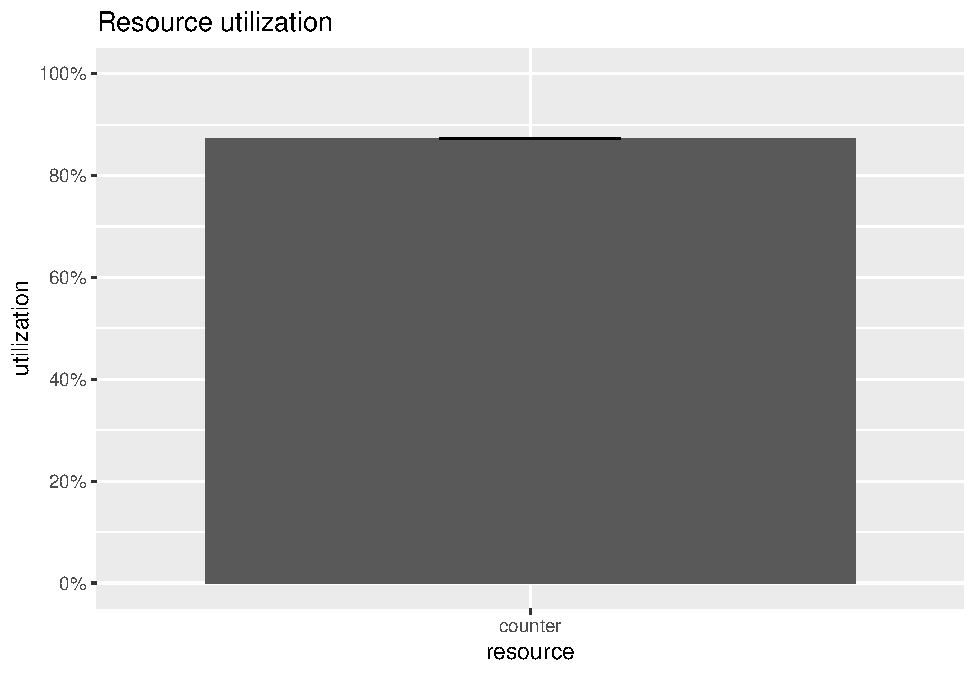
\includegraphics[width=0.8\linewidth]{SimBook_files/figure-latex/unnamed-chunk-151-1} \end{center}

So we see that our employees are busy around 90\% of the time. We can also see when they are busy as well as how many people are queuing at each moment during the simulation using the code below.

\begin{Shaded}
\begin{Highlighting}[]
\FunctionTok{plot}\NormalTok{(resources, }\AttributeTok{metric =} \StringTok{"usage"}\NormalTok{,}\AttributeTok{steps=}\NormalTok{T)}
\end{Highlighting}
\end{Shaded}

\begin{center}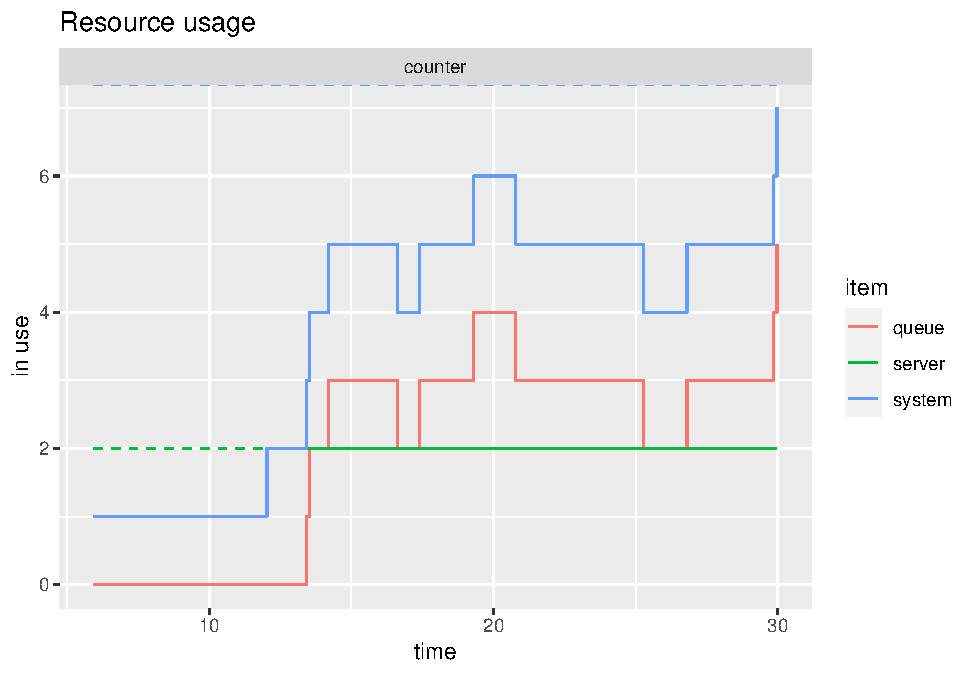
\includegraphics[width=0.8\linewidth]{SimBook_files/figure-latex/unnamed-chunk-152-1} \end{center}

The green line reports the number of employees busy and we can see that most of the time they are both busy. The red line reports the number of people queuing and waiting to be served. The blue line is the total number of customers in the system: those queuing plus those being served.

\hypertarget{replication}{%
\section{Replication}\label{replication}}

For all previous examples, we ran a unique simulation and observed the results. As we have already learned, these results are affected by randomness and different runs will show different results.

Consider the last simulation we implemented where customers arrive at the shop where we have two counters. We can simulate the system 1000 times using the following code. We will not include \texttt{log} since otherwise the output will become cluttered.

\begin{Shaded}
\begin{Highlighting}[]
\NormalTok{customer }\OtherTok{\textless{}{-}}
  \FunctionTok{trajectory}\NormalTok{(}\StringTok{"Customer\textquotesingle{}s path"}\NormalTok{) }\SpecialCharTok{\%\textgreater{}\%}
  \FunctionTok{seize}\NormalTok{(}\StringTok{"counter"}\NormalTok{) }\SpecialCharTok{\%\textgreater{}\%}
  \FunctionTok{timeout}\NormalTok{(}\ControlFlowTok{function}\NormalTok{() }\FunctionTok{rnorm}\NormalTok{(}\DecValTok{1}\NormalTok{,}\DecValTok{10}\NormalTok{,}\DecValTok{2}\NormalTok{)) }\SpecialCharTok{\%\textgreater{}\%}
  \FunctionTok{release}\NormalTok{(}\StringTok{"counter"}\NormalTok{) }


\NormalTok{envs }\OtherTok{\textless{}{-}} \FunctionTok{lapply}\NormalTok{(}\DecValTok{1}\SpecialCharTok{:}\DecValTok{100}\NormalTok{, }\ControlFlowTok{function}\NormalTok{(i) \{}
    \FunctionTok{simmer}\NormalTok{(}\StringTok{"shop"}\NormalTok{) }\SpecialCharTok{\%\textgreater{}\%} 
    \FunctionTok{add\_resource}\NormalTok{(}\StringTok{"counter"}\NormalTok{,}\DecValTok{2}\NormalTok{) }\SpecialCharTok{\%\textgreater{}\%}
    \FunctionTok{add\_generator}\NormalTok{(}\StringTok{"Customer"}\NormalTok{, customer, }\ControlFlowTok{function}\NormalTok{() }\FunctionTok{rexp}\NormalTok{(}\DecValTok{1}\NormalTok{, }\DecValTok{1}\SpecialCharTok{/}\DecValTok{5}\NormalTok{)) }\SpecialCharTok{\%\textgreater{}\%}
    \FunctionTok{run}\NormalTok{(}\AttributeTok{until=}\DecValTok{240}\NormalTok{)}
\NormalTok{\}}
\NormalTok{)}
\end{Highlighting}
\end{Shaded}

Now \texttt{envs} stores the output of simulating the behavior of the shop for 4 hours 100 times.

We can summarize the results of these simulations using the \texttt{simmer.plot} package.

\begin{Shaded}
\begin{Highlighting}[]
\FunctionTok{plot}\NormalTok{(}\FunctionTok{get\_mon\_resources}\NormalTok{(envs), }\AttributeTok{metric =} \StringTok{"utilization"}\NormalTok{)}
\end{Highlighting}
\end{Shaded}

\begin{center}\includegraphics[width=0.5\linewidth]{SimBook_files/figure-latex/unnamed-chunk-154-1} \end{center}

Compared to previous plots we now notice that the output also has something that resembles a boxplot which tells us what was the utilization of the resource in different simulation runs.

We can also assess how busy were the employees in different simulations. As the shop opens the two employees become more and more busy and at the end of the four hours they are busy almost all the time.

\begin{Shaded}
\begin{Highlighting}[]
\FunctionTok{plot}\NormalTok{(}\FunctionTok{get\_mon\_resources}\NormalTok{(envs), }\AttributeTok{metric =} \StringTok{"usage"}\NormalTok{, }\AttributeTok{items =} \StringTok{"server"}\NormalTok{)}
\end{Highlighting}
\end{Shaded}

\includegraphics{SimBook_files/figure-latex/unnamed-chunk-155-1.pdf}

Similarly, we can look at how long do customers queue in our shop.

\begin{Shaded}
\begin{Highlighting}[]
\FunctionTok{plot}\NormalTok{(}\FunctionTok{get\_mon\_arrivals}\NormalTok{(envs), }\AttributeTok{metric =} \StringTok{"waiting\_time"}\NormalTok{)}
\end{Highlighting}
\end{Shaded}

\begin{verbatim}
## `geom_smooth()` using method = 'gam' and formula 'y ~ s(x, bs = "cs")'
\end{verbatim}

\includegraphics{SimBook_files/figure-latex/unnamed-chunk-156-1.pdf}

Each black line represents a single simulation and the blue line gives an overall representation of the simulation. We can see that the waiting time seems to be linearly increasing with time.

\hypertarget{the-donut-shop---advanced-features}{%
\section{The donut shop - advanced features}\label{the-donut-shop---advanced-features}}

In many situations there is a system of priority service. Those customers with high priority are served first, those with low priority must wait. In some cases, preemptive priority will even allow a high-priority customer to interrupt the service of one with a lower priority.

\texttt{Simmer} implements priority requests with an extra integer priority argument to \texttt{add\_generator()}. By default, priority is zero; higher integers have higher priority.

\hypertarget{priority-customers-without-preemption}{%
\subsection{Priority customers without preemption}\label{priority-customers-without-preemption}}

Suppose the donut shop have priority customers that when arrive at the shop, are served as soon as possible. We make the assumption that they arrive

\begin{Shaded}
\begin{Highlighting}[]
\NormalTok{customer }\OtherTok{\textless{}{-}}
  \FunctionTok{trajectory}\NormalTok{(}\StringTok{"Customer\textquotesingle{}s path"}\NormalTok{) }\SpecialCharTok{\%\textgreater{}\%}
  \FunctionTok{log\_}\NormalTok{(}\StringTok{"Here I am"}\NormalTok{) }\SpecialCharTok{\%\textgreater{}\%}
  \FunctionTok{seize}\NormalTok{(}\StringTok{"counter"}\NormalTok{) }\SpecialCharTok{\%\textgreater{}\%}
  \FunctionTok{timeout}\NormalTok{(}\ControlFlowTok{function}\NormalTok{() }\FunctionTok{rnorm}\NormalTok{(}\DecValTok{1}\NormalTok{,}\DecValTok{10}\NormalTok{,}\DecValTok{2}\NormalTok{)) }\SpecialCharTok{\%\textgreater{}\%}
  \FunctionTok{release}\NormalTok{(}\StringTok{"counter"}\NormalTok{) }\SpecialCharTok{\%\textgreater{}\%}
   \FunctionTok{log\_}\NormalTok{(}\StringTok{"Finished"}\NormalTok{)}

\NormalTok{shop }\OtherTok{\textless{}{-}}
  \FunctionTok{simmer}\NormalTok{(}\StringTok{"shop"}\NormalTok{) }\SpecialCharTok{\%\textgreater{}\%}
  \FunctionTok{add\_resource}\NormalTok{(}\StringTok{"counter"}\NormalTok{) }\SpecialCharTok{\%\textgreater{}\%}
  \FunctionTok{add\_generator}\NormalTok{(}\StringTok{"Customer"}\NormalTok{, customer, }\ControlFlowTok{function}\NormalTok{() }\FunctionTok{rexp}\NormalTok{(}\DecValTok{1}\NormalTok{, }\DecValTok{1}\SpecialCharTok{/}\DecValTok{5}\NormalTok{)) }\SpecialCharTok{\%\textgreater{}\%}
\FunctionTok{add\_generator}\NormalTok{(}\StringTok{"Priority\_Customer"}\NormalTok{, customer, }\ControlFlowTok{function}\NormalTok{() }\FunctionTok{rexp}\NormalTok{(}\DecValTok{1}\NormalTok{, }\DecValTok{1}\SpecialCharTok{/}\DecValTok{15}\NormalTok{), }\AttributeTok{priority =} \DecValTok{1}\NormalTok{)}

\FunctionTok{set.seed}\NormalTok{(}\DecValTok{2021}\NormalTok{)}
\NormalTok{shop }\SpecialCharTok{\%\textgreater{}\%} \FunctionTok{run}\NormalTok{(}\AttributeTok{until =} \DecValTok{45}\NormalTok{)}
\end{Highlighting}
\end{Shaded}

\begin{verbatim}
## 5.92531: Customer0: Here I am
## 7.28854: Customer1: Here I am
## 11.0879: Customer2: Here I am
## 14.2421: Customer3: Here I am
## 14.3366: Customer4: Here I am
## 15.0111: Customer5: Here I am
## 16.9819: Customer0: Finished
## 18.2117: Customer6: Here I am
## 18.3019: Priority_Customer0: Here I am
## 20.1029: Customer7: Here I am
## 21.0334: Customer8: Here I am
## 21.7555: Customer9: Here I am
## 24.807: Customer10: Here I am
## 24.9206: Customer11: Here I am
## 25.6428: Customer1: Finished
## 28.047: Customer12: Here I am
## 28.879: Customer13: Here I am
## 32.9443: Customer14: Here I am
## 35.9055: Priority_Customer0: Finished
## 36.8793: Customer15: Here I am
## 40.846: Priority_Customer1: Here I am
\end{verbatim}

\begin{verbatim}
## simmer environment: shop | now: 45 | next: 47.5452877648588
## { Monitor: in memory }
## { Resource: counter | monitored: TRUE | server status: 1(1) | queue status: 14(Inf) }
## { Source: Customer | monitored: 1 | n_generated: 17 }
## { Source: Priority_Customer | monitored: 1 | n_generated: 3 }
\end{verbatim}

From the output we can see that whenever a priority customer joins the queue he is sold donuts as soon as the employee becomes available.

\hypertarget{priority-customers-with-preemption}{%
\subsection{Priority customers with preemption}\label{priority-customers-with-preemption}}

Now we allow priority customers to have preemptive priority. They will displace any customer in service when they arrive. That customer will resume when they finish (unless higher priority customers intervene). This requires only a change to one line of the program, adding the argument, \texttt{preemptive\ =\ TRUE} to the \texttt{add\_resource} function call.

\begin{Shaded}
\begin{Highlighting}[]
\NormalTok{shop }\OtherTok{\textless{}{-}}
  \FunctionTok{simmer}\NormalTok{(}\StringTok{"shop"}\NormalTok{) }\SpecialCharTok{\%\textgreater{}\%}
  \FunctionTok{add\_resource}\NormalTok{(}\StringTok{"counter"}\NormalTok{, }\AttributeTok{preemptive =} \ConstantTok{TRUE}\NormalTok{) }\SpecialCharTok{\%\textgreater{}\%}
  \FunctionTok{add\_generator}\NormalTok{(}\StringTok{"Customer"}\NormalTok{, customer, }\ControlFlowTok{function}\NormalTok{() }\FunctionTok{rexp}\NormalTok{(}\DecValTok{1}\NormalTok{, }\DecValTok{1}\SpecialCharTok{/}\DecValTok{5}\NormalTok{)) }\SpecialCharTok{\%\textgreater{}\%}
\FunctionTok{add\_generator}\NormalTok{(}\StringTok{"Priority\_Customer"}\NormalTok{, customer, }\ControlFlowTok{function}\NormalTok{() }\FunctionTok{rexp}\NormalTok{(}\DecValTok{1}\NormalTok{, }\DecValTok{1}\SpecialCharTok{/}\DecValTok{15}\NormalTok{), }\AttributeTok{priority =} \DecValTok{1}\NormalTok{)}

\FunctionTok{set.seed}\NormalTok{(}\DecValTok{2021}\NormalTok{)}
\NormalTok{shop }\SpecialCharTok{\%\textgreater{}\%} \FunctionTok{run}\NormalTok{(}\AttributeTok{until =} \DecValTok{45}\NormalTok{)}
\end{Highlighting}
\end{Shaded}

\begin{verbatim}
## 5.92531: Customer0: Here I am
## 7.28854: Customer1: Here I am
## 11.0879: Customer2: Here I am
## 14.2421: Customer3: Here I am
## 14.3366: Customer4: Here I am
## 15.0111: Customer5: Here I am
## 16.9819: Customer0: Finished
## 18.2117: Customer6: Here I am
## 18.3019: Priority_Customer0: Here I am
## 20.1029: Customer7: Here I am
## 23.9383: Customer8: Here I am
## 24.6604: Customer9: Here I am
## 27.7119: Customer10: Here I am
## 27.8255: Customer11: Here I am
## 30.9519: Customer12: Here I am
## 31.4746: Customer13: Here I am
## 31.6998: Priority_Customer0: Finished
## 39.0407: Customer1: Finished
## 39.2381: Customer14: Here I am
## 40.846: Priority_Customer1: Here I am
\end{verbatim}

\begin{verbatim}
## simmer environment: shop | now: 45 | next: 45.2787752879948
## { Monitor: in memory }
## { Resource: counter | monitored: TRUE | server status: 1(1) | queue status: 13(Inf) }
## { Source: Customer | monitored: 1 | n_generated: 16 }
## { Source: Priority_Customer | monitored: 1 | n_generated: 3 }
\end{verbatim}

In this other case, priority customers are served straight away. The customer that was served when the priority customer arrived resumes is service as soon as the priority customer finishes.

\hypertarget{balking-customers}{%
\subsection{Balking customers}\label{balking-customers}}

Balking occurs when a customer refuses to join a queue if it is too long. Suppose that if there is one customer queuing in our shop then customers do not join the queue and leave. We can implement this by setting the \texttt{queue\_size} option of \texttt{add\_resource} and by adding some options of the \texttt{seize} function. Let's consider the following code.

\begin{Shaded}
\begin{Highlighting}[]
\NormalTok{customer }\OtherTok{\textless{}{-}}
  \FunctionTok{trajectory}\NormalTok{(}\StringTok{"Customer\textquotesingle{}s path"}\NormalTok{) }\SpecialCharTok{\%\textgreater{}\%}
  \FunctionTok{log\_}\NormalTok{(}\StringTok{"Here I am"}\NormalTok{) }\SpecialCharTok{\%\textgreater{}\%}
  \FunctionTok{seize}\NormalTok{(}\StringTok{"counter"}\NormalTok{, }\AttributeTok{continue =} \ConstantTok{FALSE}\NormalTok{, }\AttributeTok{reject =} 
          \FunctionTok{trajectory}\NormalTok{(}\StringTok{"Balked customer"}\NormalTok{) }\SpecialCharTok{\%\textgreater{}\%} \FunctionTok{log\_}\NormalTok{(}\StringTok{"Balking"}\NormalTok{) ) }\SpecialCharTok{\%\textgreater{}\%}
  \FunctionTok{timeout}\NormalTok{(}\ControlFlowTok{function}\NormalTok{() }\FunctionTok{rnorm}\NormalTok{(}\DecValTok{1}\NormalTok{,}\DecValTok{10}\NormalTok{,}\DecValTok{2}\NormalTok{)) }\SpecialCharTok{\%\textgreater{}\%}
  \FunctionTok{release}\NormalTok{(}\StringTok{"counter"}\NormalTok{) }\SpecialCharTok{\%\textgreater{}\%}
   \FunctionTok{log\_}\NormalTok{(}\StringTok{"Finished"}\NormalTok{)}

\NormalTok{shop }\OtherTok{\textless{}{-}}
  \FunctionTok{simmer}\NormalTok{(}\StringTok{"shop"}\NormalTok{) }\SpecialCharTok{\%\textgreater{}\%}
  \FunctionTok{add\_resource}\NormalTok{(}\StringTok{"counter"}\NormalTok{, }\AttributeTok{queue\_size =} \DecValTok{1}\NormalTok{) }\SpecialCharTok{\%\textgreater{}\%}
  \FunctionTok{add\_generator}\NormalTok{(}\StringTok{"Customer"}\NormalTok{, customer,}
                \ControlFlowTok{function}\NormalTok{() }\FunctionTok{rexp}\NormalTok{(}\DecValTok{1}\NormalTok{, }\DecValTok{1}\SpecialCharTok{/}\DecValTok{5}\NormalTok{))}
\end{Highlighting}
\end{Shaded}

The input \texttt{queue\_size} is self-explanatory and simply sets how many people can queue for the counter. In the \texttt{seize} function we set the inputs \texttt{continue} and \texttt{reject}. With \texttt{continue\ =\ FALSE} we are saying that a rejected customer does not follow the rest of the trajectory. With \texttt{reject} we are specifying what trajectory the rejected customer will follow.

Let's run the simulation.

\begin{Shaded}
\begin{Highlighting}[]
\FunctionTok{set.seed}\NormalTok{(}\DecValTok{2021}\NormalTok{)}
\NormalTok{shop }\SpecialCharTok{\%\textgreater{}\%} \FunctionTok{run}\NormalTok{(}\AttributeTok{until =} \DecValTok{45}\NormalTok{)}
\end{Highlighting}
\end{Shaded}

\begin{verbatim}
## 5.92531: Customer0: Here I am
## 12.0259: Customer1: Here I am
## 13.4303: Customer2: Here I am
## 13.4303: Customer2: Balking
## 16.6226: Customer0: Finished
## 17.2296: Customer3: Here I am
## 28.4187: Customer1: Finished
## 36.649: Customer4: Here I am
## 38.7585: Customer3: Finished
## 40.1462: Customer5: Here I am
## 40.6299: Customer6: Here I am
## 40.6299: Customer6: Balking
## 41.5604: Customer7: Here I am
## 41.5604: Customer7: Balking
## 42.2825: Customer8: Here I am
## 42.2825: Customer8: Balking
\end{verbatim}

\begin{verbatim}
## simmer environment: shop | now: 45 | next: 45.3340111165536
## { Monitor: in memory }
## { Resource: counter | monitored: TRUE | server status: 1(1) | queue status: 1(1) }
## { Source: Customer | monitored: 1 | n_generated: 10 }
\end{verbatim}

So now we see that often customers just leave the shop because they decide not to queue. We can count how many of them left for balking using:

\begin{Shaded}
\begin{Highlighting}[]
\FunctionTok{sum}\NormalTok{(}\FunctionTok{get\_mon\_arrivals}\NormalTok{(shop)}\SpecialCharTok{$}\NormalTok{activity\_time }\SpecialCharTok{==} \DecValTok{0}\NormalTok{)}
\end{Highlighting}
\end{Shaded}

\begin{verbatim}
## [1] 4
\end{verbatim}

and the hourly rate at which they leave

\begin{Shaded}
\begin{Highlighting}[]
\FunctionTok{sum}\NormalTok{(}\FunctionTok{get\_mon\_arrivals}\NormalTok{(shop)}\SpecialCharTok{$}\NormalTok{activity\_time }\SpecialCharTok{==} \DecValTok{0}\NormalTok{)}\SpecialCharTok{/}\FunctionTok{now}\NormalTok{(shop)}\SpecialCharTok{*}\DecValTok{60}
\end{Highlighting}
\end{Shaded}

\begin{verbatim}
## [1] 5.333333
\end{verbatim}

\hypertarget{reneging-or-abandoning-customers}{%
\subsection{Reneging (or abandoning) customers}\label{reneging-or-abandoning-customers}}

Often in practice an impatient customer will leave the queue before being served. Simmer can model this reneging behaviour using the \texttt{renege\_in()} function in a trajectory. This defines the maximum time that a customer will wait before reneging, as well as an `out' trajectory for them to follow when they renege.

If the customer reaches the server before reneging, then their impatience must be cancelled with the \texttt{renege\_abort()} function.

\begin{Shaded}
\begin{Highlighting}[]
\NormalTok{customer }\OtherTok{\textless{}{-}}
  \FunctionTok{trajectory}\NormalTok{(}\StringTok{"Customer\textquotesingle{}s path"}\NormalTok{) }\SpecialCharTok{\%\textgreater{}\%}
  \FunctionTok{log\_}\NormalTok{(}\StringTok{"Here I am"}\NormalTok{) }\SpecialCharTok{\%\textgreater{}\%}
  \FunctionTok{renege\_in}\NormalTok{(}\ControlFlowTok{function}\NormalTok{() }\FunctionTok{rnorm}\NormalTok{(}\DecValTok{1}\NormalTok{,}\DecValTok{5}\NormalTok{,}\DecValTok{1}\NormalTok{),}
            \AttributeTok{out =} \FunctionTok{trajectory}\NormalTok{(}\StringTok{"Reneging customer"}\NormalTok{) }\SpecialCharTok{\%\textgreater{}\%}
              \FunctionTok{log\_}\NormalTok{(}\StringTok{"I am off"}\NormalTok{)) }\SpecialCharTok{\%\textgreater{}\%}
  \FunctionTok{seize}\NormalTok{(}\StringTok{"counter"}\NormalTok{) }\SpecialCharTok{\%\textgreater{}\%}
  \FunctionTok{renege\_abort}\NormalTok{() }\SpecialCharTok{\%\textgreater{}\%}
  \FunctionTok{timeout}\NormalTok{(}\ControlFlowTok{function}\NormalTok{() }\FunctionTok{rnorm}\NormalTok{(}\DecValTok{1}\NormalTok{,}\DecValTok{10}\NormalTok{,}\DecValTok{2}\NormalTok{)) }\SpecialCharTok{\%\textgreater{}\%}
  \FunctionTok{release}\NormalTok{(}\StringTok{"counter"}\NormalTok{) }\SpecialCharTok{\%\textgreater{}\%}
   \FunctionTok{log\_}\NormalTok{(}\StringTok{"Finished"}\NormalTok{)}

\NormalTok{shop }\OtherTok{\textless{}{-}}
  \FunctionTok{simmer}\NormalTok{(}\StringTok{"shop"}\NormalTok{) }\SpecialCharTok{\%\textgreater{}\%}
  \FunctionTok{add\_resource}\NormalTok{(}\StringTok{"counter"}\NormalTok{) }\SpecialCharTok{\%\textgreater{}\%}
  \FunctionTok{add\_generator}\NormalTok{(}\StringTok{"Customer"}\NormalTok{, customer, }\ControlFlowTok{function}\NormalTok{() }\FunctionTok{rexp}\NormalTok{(}\DecValTok{1}\NormalTok{, }\DecValTok{1}\SpecialCharTok{/}\DecValTok{5}\NormalTok{))}

\FunctionTok{run}\NormalTok{(shop, }\AttributeTok{until =} \DecValTok{45}\NormalTok{)}
\end{Highlighting}
\end{Shaded}

\begin{verbatim}
## 0.113593: Customer0: Here I am
## 0.892989: Customer1: Here I am
## 7.40631: Customer1: I am off
## 9.74378: Customer2: Here I am
## 10.2131: Customer3: Here I am
## 13.0758: Customer0: Finished
## 16.4212: Customer3: I am off
## 24.9321: Customer2: Finished
## 27.4101: Customer4: Here I am
## 27.7221: Customer5: Here I am
## 27.808: Customer6: Here I am
## 32.6284: Customer5: I am off
## 32.8674: Customer6: I am off
## 34.1951: Customer7: Here I am
## 36.7021: Customer4: Finished
\end{verbatim}

\begin{verbatim}
## simmer environment: shop | now: 45 | next: 45.8000847848882
## { Monitor: in memory }
## { Resource: counter | monitored: TRUE | server status: 1(1) | queue status: 0(Inf) }
## { Source: Customer | monitored: 1 | n_generated: 9 }
\end{verbatim}

\hypertarget{several-counters-with-individual-queues}{%
\subsection{Several counters with individual queues}\label{several-counters-with-individual-queues}}

Each counter is now assumed to have its own queue. The programming is more complicated because the customer has to decide which queue to join. The obvious technique is to make each counter a separate resource.

In practice, a customer might join the shortest queue. We implement this behaviour by first selecting the shortest queue, using the \texttt{select} function. Then we use \texttt{seize\_selected} to enter the chosen queue, and later \texttt{release\_selected}.

The rest of the program is the same as before.

\begin{Shaded}
\begin{Highlighting}[]
\FunctionTok{set.seed}\NormalTok{(}\DecValTok{2021}\NormalTok{)}
\NormalTok{customer }\OtherTok{\textless{}{-}}
  \FunctionTok{trajectory}\NormalTok{(}\StringTok{"Customer\textquotesingle{}s path"}\NormalTok{) }\SpecialCharTok{\%\textgreater{}\%}
  \FunctionTok{log\_}\NormalTok{(}\StringTok{"Here I am"}\NormalTok{) }\SpecialCharTok{\%\textgreater{}\%}
  \FunctionTok{select}\NormalTok{(}\FunctionTok{c}\NormalTok{(}\StringTok{"counter1"}\NormalTok{, }\StringTok{"counter2"}\NormalTok{), }\AttributeTok{policy =} \StringTok{"shortest{-}queue"}\NormalTok{) }\SpecialCharTok{\%\textgreater{}\%}
  \FunctionTok{seize\_selected}\NormalTok{() }\SpecialCharTok{\%\textgreater{}\%}
  \FunctionTok{timeout}\NormalTok{(}\ControlFlowTok{function}\NormalTok{() }\FunctionTok{rnorm}\NormalTok{(}\DecValTok{1}\NormalTok{,}\DecValTok{10}\NormalTok{,}\DecValTok{2}\NormalTok{)) }\SpecialCharTok{\%\textgreater{}\%}
  \FunctionTok{release\_selected}\NormalTok{() }\SpecialCharTok{\%\textgreater{}\%}
   \FunctionTok{log\_}\NormalTok{(}\StringTok{"Finished"}\NormalTok{)}

\NormalTok{shop }\OtherTok{\textless{}{-}}
  \FunctionTok{simmer}\NormalTok{(}\StringTok{"shop"}\NormalTok{) }\SpecialCharTok{\%\textgreater{}\%}
  \FunctionTok{add\_resource}\NormalTok{(}\StringTok{"counter1"}\NormalTok{, }\DecValTok{1}\NormalTok{) }\SpecialCharTok{\%\textgreater{}\%}
  \FunctionTok{add\_resource}\NormalTok{(}\StringTok{"counter2"}\NormalTok{, }\DecValTok{1}\NormalTok{) }\SpecialCharTok{\%\textgreater{}\%}
  \FunctionTok{add\_generator}\NormalTok{(}\StringTok{"Customer"}\NormalTok{, customer, }\ControlFlowTok{function}\NormalTok{() }\FunctionTok{rexp}\NormalTok{(}\DecValTok{1}\NormalTok{, }\DecValTok{1}\SpecialCharTok{/}\DecValTok{5}\NormalTok{))}

\FunctionTok{run}\NormalTok{(shop, }\AttributeTok{until =} \DecValTok{45}\NormalTok{)}
\end{Highlighting}
\end{Shaded}

\begin{verbatim}
## 5.92531: Customer0: Here I am
## 12.0259: Customer1: Here I am
## 13.4303: Customer2: Here I am
## 13.5248: Customer3: Here I am
## 14.1994: Customer4: Here I am
## 16.6226: Customer0: Finished
## 17.3999: Customer5: Here I am
## 19.2911: Customer6: Here I am
## 20.7802: Customer1: Finished
## 25.2835: Customer2: Finished
## 26.8058: Customer7: Here I am
## 29.8574: Customer8: Here I am
## 29.971: Customer9: Here I am
## 33.0974: Customer10: Here I am
## 33.62: Customer11: Here I am
## 34.0487: Customer4: Finished
## 34.1781: Customer3: Finished
## 41.3835: Customer12: Here I am
## 42.2932: Customer6: Finished
\end{verbatim}

\begin{verbatim}
## simmer environment: shop | now: 45 | next: 45.3185680974989
## { Monitor: in memory }
## { Resource: counter1 | monitored: TRUE | server status: 1(1) | queue status: 3(Inf) }
## { Resource: counter2 | monitored: TRUE | server status: 1(1) | queue status: 2(Inf) }
## { Source: Customer | monitored: 1 | n_generated: 14 }
\end{verbatim}

There are several policies implemented internally
that can be accessed by name:

\begin{itemize}
\item
  \texttt{shortest-queue}: The resource with the shortest queue is selected.
\item
  \texttt{round-robin}: Resources will be selected in a cyclical nature.
\item
  \texttt{first-available}: The first available resource is selected.
\item
  \texttt{random} A resource is randomly selected.
\end{itemize}

\hypertarget{opening-times}{%
\subsection{Opening times}\label{opening-times}}

Customers arrive at random, some of them getting to the shop before the door is opened by a doorman. They wait for the door to be opened and then rush in and queue to be served.

This model defines the door as a resource, just like the counter. The capacity of the door is defined according to the \texttt{schedule} function, so that it has zero capacity when it is shut, and infinite capacity when it is open. Customers `seize' the door and must then wait until it has capacity to `serve' them. Once it is available, all waiting customers are `served' immediately (i.e.~they pass through the door). There is no timeout between `seizing' and `releasing' the door.

\begin{Shaded}
\begin{Highlighting}[]
\NormalTok{customer }\OtherTok{\textless{}{-}}
  \FunctionTok{trajectory}\NormalTok{(}\StringTok{"Customer\textquotesingle{}s path"}\NormalTok{) }\SpecialCharTok{\%\textgreater{}\%}
  \FunctionTok{log\_}\NormalTok{(}\ControlFlowTok{function}\NormalTok{()}
    \ControlFlowTok{if}\NormalTok{ (}\FunctionTok{get\_capacity}\NormalTok{(shop, }\StringTok{"door"}\NormalTok{) }\SpecialCharTok{==} \DecValTok{0}\NormalTok{)}
      \StringTok{"Here I am but the door is shut."}
    \ControlFlowTok{else} \StringTok{"Here I am and the door is open."}
\NormalTok{  ) }\SpecialCharTok{\%\textgreater{}\%}
  \FunctionTok{seize}\NormalTok{(}\StringTok{"door"}\NormalTok{) }\SpecialCharTok{\%\textgreater{}\%}
  \FunctionTok{log\_}\NormalTok{(}\StringTok{"I can go in!"}\NormalTok{) }\SpecialCharTok{\%\textgreater{}\%}
  \FunctionTok{release}\NormalTok{(}\StringTok{"door"}\NormalTok{) }\SpecialCharTok{\%\textgreater{}\%}
  \FunctionTok{seize}\NormalTok{(}\StringTok{"counter"}\NormalTok{) }\SpecialCharTok{\%\textgreater{}\%}
  \FunctionTok{timeout}\NormalTok{(}\ControlFlowTok{function}\NormalTok{() \{}\FunctionTok{rexp}\NormalTok{(}\DecValTok{1}\NormalTok{, }\DecValTok{10}\NormalTok{)\}) }\SpecialCharTok{\%\textgreater{}\%}
  \FunctionTok{release}\NormalTok{(}\StringTok{"counter"}\NormalTok{)}

\NormalTok{door\_schedule }\OtherTok{\textless{}{-}} \FunctionTok{schedule}\NormalTok{(}\FunctionTok{c}\NormalTok{(}\DecValTok{1}\NormalTok{,}\DecValTok{7}\NormalTok{,}\DecValTok{9}\NormalTok{,}\DecValTok{13}\NormalTok{), }\FunctionTok{c}\NormalTok{(}\ConstantTok{Inf}\NormalTok{,}\DecValTok{0}\NormalTok{,}\ConstantTok{Inf}\NormalTok{,}\DecValTok{0}\NormalTok{), }\AttributeTok{period =} \DecValTok{13}\NormalTok{)}

\NormalTok{shop }\OtherTok{\textless{}{-}}
  \FunctionTok{simmer}\NormalTok{(}\StringTok{"shop"}\NormalTok{) }\SpecialCharTok{\%\textgreater{}\%}
  \FunctionTok{add\_resource}\NormalTok{(}\StringTok{"door"}\NormalTok{, }\AttributeTok{capacity =}\NormalTok{ door\_schedule) }\SpecialCharTok{\%\textgreater{}\%}
  \FunctionTok{add\_resource}\NormalTok{(}\StringTok{"counter"}\NormalTok{) }\SpecialCharTok{\%\textgreater{}\%}
  \FunctionTok{add\_generator}\NormalTok{(}\StringTok{"Customer"}\NormalTok{, customer, }\ControlFlowTok{function}\NormalTok{() }\FunctionTok{rexp}\NormalTok{(}\DecValTok{1}\NormalTok{, }\DecValTok{1}\NormalTok{))}

\NormalTok{shop }\SpecialCharTok{\%\textgreater{}\%} \FunctionTok{run}\NormalTok{(}\DecValTok{26}\NormalTok{)}
\end{Highlighting}
\end{Shaded}

\begin{verbatim}
## 3.53354: Customer0: Here I am and the door is open.
## 3.53354: Customer0: I can go in!
## 6.97294: Customer1: Here I am and the door is open.
## 6.97294: Customer1: I can go in!
## 7.05686: Customer2: Here I am but the door is shut.
## 9: Customer2: I can go in!
## 9.30068: Customer3: Here I am and the door is open.
## 9.30068: Customer3: I can go in!
## 10.4405: Customer4: Here I am and the door is open.
## 10.4405: Customer4: I can go in!
## 11.3978: Customer5: Here I am and the door is open.
## 11.3978: Customer5: I can go in!
## 15.4491: Customer6: Here I am and the door is open.
## 15.4491: Customer6: I can go in!
## 17.7096: Customer7: Here I am and the door is open.
## 17.7096: Customer7: I can go in!
## 18.4016: Customer8: Here I am and the door is open.
## 18.4016: Customer8: I can go in!
## 19.1858: Customer9: Here I am and the door is open.
## 19.1858: Customer9: I can go in!
## 22.0271: Customer10: Here I am and the door is open.
## 22.0271: Customer10: I can go in!
## 22.9206: Customer11: Here I am and the door is open.
## 22.9206: Customer11: I can go in!
## 24.0738: Customer12: Here I am and the door is open.
## 24.0738: Customer12: I can go in!
## 24.9154: Customer13: Here I am and the door is open.
## 24.9154: Customer13: I can go in!
## 25.3469: Customer14: Here I am and the door is open.
## 25.3469: Customer14: I can go in!
## 25.7375: Customer15: Here I am and the door is open.
## 25.7375: Customer15: I can go in!
\end{verbatim}

\begin{verbatim}
## simmer environment: shop | now: 26 | next: 26
## { Monitor: in memory }
## { Resource: door | monitored: TRUE | server status: 0(Inf) | queue status: 0(Inf) }
## { Resource: counter | monitored: TRUE | server status: 1(1) | queue status: 0(Inf) }
## { Source: Customer | monitored: 1 | n_generated: 17 }
\end{verbatim}

\hypertarget{batching-clients}{%
\subsection{Batching clients}\label{batching-clients}}

Customers arrive at random, some of them getting to the shop before the door is open. This is controlled by an automatic machine called the doorman which opens the door only at intervals of 30 minutes (it is a very secure shop). The customers wait for the door to be opened and all those waiting enter and proceed to the counter. The door is closed behind them.

One possible solution is using batching. Customers can be collected into batches of a given size, or for a given time, or whichever occurs first. Here, they are collected for periods of 30, and the number of customers in each batch is unrestricted.

After the batch is created with \texttt{batch} it is then separated with \texttt{separate}.

\begin{Shaded}
\begin{Highlighting}[]
\FunctionTok{set.seed}\NormalTok{(}\DecValTok{2021}\NormalTok{)}
\NormalTok{customer }\OtherTok{\textless{}{-}}
  \FunctionTok{trajectory}\NormalTok{(}\StringTok{"Customer\textquotesingle{}s path"}\NormalTok{) }\SpecialCharTok{\%\textgreater{}\%}
  \FunctionTok{log\_}\NormalTok{(}\StringTok{"Here I am, but the door is shut."}\NormalTok{) }\SpecialCharTok{\%\textgreater{}\%}
  \FunctionTok{batch}\NormalTok{(}\AttributeTok{n =} \ConstantTok{Inf}\NormalTok{, }\AttributeTok{timeout =} \DecValTok{30}\NormalTok{) }\SpecialCharTok{\%\textgreater{}\%}
  \FunctionTok{separate}\NormalTok{() }\SpecialCharTok{\%\textgreater{}\%}
  \FunctionTok{log\_}\NormalTok{(}\StringTok{"The door is open!"}\NormalTok{) }\SpecialCharTok{\%\textgreater{}\%}
  \FunctionTok{seize}\NormalTok{(}\StringTok{"counter"}\NormalTok{) }\SpecialCharTok{\%\textgreater{}\%}
  \FunctionTok{timeout}\NormalTok{(}\ControlFlowTok{function}\NormalTok{() \{}\FunctionTok{rexp}\NormalTok{(}\DecValTok{1}\NormalTok{, }\DecValTok{1}\SpecialCharTok{/}\DecValTok{2}\NormalTok{)\}) }\SpecialCharTok{\%\textgreater{}\%}
  \FunctionTok{release}\NormalTok{(}\StringTok{"counter"}\NormalTok{) }\SpecialCharTok{\%\textgreater{}\%}
  \FunctionTok{log\_}\NormalTok{(}\StringTok{"Finished."}\NormalTok{)}

\NormalTok{shop }\OtherTok{\textless{}{-}} \FunctionTok{simmer}\NormalTok{(}\StringTok{"shop"}\NormalTok{)}
\NormalTok{shop }\SpecialCharTok{\%\textgreater{}\%}
  \FunctionTok{add\_resource}\NormalTok{(}\StringTok{"door"}\NormalTok{) }\SpecialCharTok{\%\textgreater{}\%}
  \FunctionTok{add\_resource}\NormalTok{(}\StringTok{"counter"}\NormalTok{) }\SpecialCharTok{\%\textgreater{}\%}
  \FunctionTok{add\_generator}\NormalTok{(}\StringTok{"Customer"}\NormalTok{,}
\NormalTok{                customer, }\ControlFlowTok{function}\NormalTok{() }\FunctionTok{rexp}\NormalTok{(}\DecValTok{1}\NormalTok{, }\DecValTok{1}\SpecialCharTok{/}\DecValTok{20}\NormalTok{)) }
\end{Highlighting}
\end{Shaded}

\begin{verbatim}
## simmer environment: shop | now: 0 | next: 0
## { Monitor: in memory }
## { Resource: door | monitored: TRUE | server status: 0(1) | queue status: 0(Inf) }
## { Resource: counter | monitored: TRUE | server status: 0(1) | queue status: 0(Inf) }
## { Source: Customer | monitored: 1 | n_generated: 0 }
\end{verbatim}

\begin{Shaded}
\begin{Highlighting}[]
\NormalTok{shop }\SpecialCharTok{\%\textgreater{}\%} \FunctionTok{run}\NormalTok{(}\DecValTok{65}\NormalTok{)}
\end{Highlighting}
\end{Shaded}

\begin{verbatim}
## 23.7012: Customer0: Here I am, but the door is shut.
## 48.1037: Customer1: Here I am, but the door is shut.
## 53.5567: Customer2: Here I am, but the door is shut.
## 53.7012: Customer0: The door is open!
## 53.7012: Customer1: The door is open!
## 53.7012: Customer2: The door is open!
## 54.263: Customer0: Finished.
## 55.7827: Customer1: Finished.
## 57.0444: Customer2: Finished.
## 61.6105: Customer3: Here I am, but the door is shut.
## 61.9885: Customer4: Here I am, but the door is shut.
## 64.6866: Customer5: Here I am, but the door is shut.
\end{verbatim}

\begin{verbatim}
## simmer environment: shop | now: 65 | next: 77.4887534806737
## { Monitor: in memory }
## { Resource: door | monitored: TRUE | server status: 0(1) | queue status: 0(Inf) }
## { Resource: counter | monitored: TRUE | server status: 0(1) | queue status: 0(Inf) }
## { Source: Customer | monitored: 1 | n_generated: 7 }
\end{verbatim}

The function \texttt{balk} takes two inputs:

\begin{itemize}
\item
  \texttt{n}: the batch size;
\item
  \texttt{timeout}: set an optional timer which triggers batches every \texttt{timeout} time units even if the batch size has not been fulfilled.
\end{itemize}

\hypertarget{simulating-a-simple-health-center}{%
\section{Simulating a simple health center}\label{simulating-a-simple-health-center}}

Let's say we want to simulate an ambulatory consultation where a patient is first seen by a nurse for an intake, next by two doctors for the consultation and finally by administrative staff to schedule a follow-up appointment.

We can construct a patient trajectory which defines all these steps.

\begin{Shaded}
\begin{Highlighting}[]
\NormalTok{patient }\OtherTok{\textless{}{-}} \FunctionTok{trajectory}\NormalTok{(}\StringTok{"patients\textquotesingle{} path"}\NormalTok{) }\SpecialCharTok{\%\textgreater{}\%}
  \DocumentationTok{\#\# add an intake activity }
  \FunctionTok{seize}\NormalTok{(}\StringTok{"nurse"}\NormalTok{, }\DecValTok{1}\NormalTok{) }\SpecialCharTok{\%\textgreater{}\%}
  \FunctionTok{timeout}\NormalTok{(}\ControlFlowTok{function}\NormalTok{() }\FunctionTok{rnorm}\NormalTok{(}\DecValTok{1}\NormalTok{, }\DecValTok{15}\NormalTok{)) }\SpecialCharTok{\%\textgreater{}\%}
  \FunctionTok{release}\NormalTok{(}\StringTok{"nurse"}\NormalTok{, }\DecValTok{1}\NormalTok{) }\SpecialCharTok{\%\textgreater{}\%}
  \DocumentationTok{\#\# add a consultation activity}
  \FunctionTok{seize}\NormalTok{(}\StringTok{"doctor"}\NormalTok{, }\DecValTok{2}\NormalTok{) }\SpecialCharTok{\%\textgreater{}\%}
  \FunctionTok{timeout}\NormalTok{(}\ControlFlowTok{function}\NormalTok{() }\FunctionTok{rnorm}\NormalTok{(}\DecValTok{1}\NormalTok{, }\DecValTok{20}\NormalTok{)) }\SpecialCharTok{\%\textgreater{}\%}
  \FunctionTok{release}\NormalTok{(}\StringTok{"doctor"}\NormalTok{, }\DecValTok{2}\NormalTok{) }\SpecialCharTok{\%\textgreater{}\%}
  \DocumentationTok{\#\# add a planning activity}
  \FunctionTok{seize}\NormalTok{(}\StringTok{"administration"}\NormalTok{, }\DecValTok{1}\NormalTok{) }\SpecialCharTok{\%\textgreater{}\%}
  \FunctionTok{timeout}\NormalTok{(}\ControlFlowTok{function}\NormalTok{() }\FunctionTok{rnorm}\NormalTok{(}\DecValTok{1}\NormalTok{, }\DecValTok{5}\NormalTok{)) }\SpecialCharTok{\%\textgreater{}\%}
  \FunctionTok{release}\NormalTok{(}\StringTok{"administration"}\NormalTok{, }\DecValTok{1}\NormalTok{)}
\end{Highlighting}
\end{Shaded}

\begin{Shaded}
\begin{Highlighting}[]
\FunctionTok{plot}\NormalTok{(patient)}
\end{Highlighting}
\end{Shaded}

\includegraphics{SimBook_files/figure-latex/unnamed-chunk-168-1.pdf}

Once the trajectory is known, you may attach arrivals to it and define the resources needed. In the example below, three types of resources are added: the nurse and administration resources, each one with a capacity of 2, and the doctor resource, with a capacity of 4. The last method adds a generator of arrivals (patients) following the trajectory patient. The time between patients is about 5 minutes.

Let's run the simulation using replication.

\begin{Shaded}
\begin{Highlighting}[]
\NormalTok{envs }\OtherTok{\textless{}{-}} \FunctionTok{lapply}\NormalTok{(}\DecValTok{1}\SpecialCharTok{:}\DecValTok{100}\NormalTok{, }\ControlFlowTok{function}\NormalTok{(i) \{}
\FunctionTok{simmer}\NormalTok{(}\StringTok{"health center"}\NormalTok{) }\SpecialCharTok{\%\textgreater{}\%}
  \FunctionTok{add\_resource}\NormalTok{(}\StringTok{"nurse"}\NormalTok{, }\DecValTok{3}\NormalTok{) }\SpecialCharTok{\%\textgreater{}\%}
  \FunctionTok{add\_resource}\NormalTok{(}\StringTok{"doctor"}\NormalTok{, }\DecValTok{4}\NormalTok{) }\SpecialCharTok{\%\textgreater{}\%}
  \FunctionTok{add\_resource}\NormalTok{(}\StringTok{"administration"}\NormalTok{, }\DecValTok{2}\NormalTok{) }\SpecialCharTok{\%\textgreater{}\%}
  \FunctionTok{add\_generator}\NormalTok{(}\StringTok{"patient"}\NormalTok{, patient, }\ControlFlowTok{function}\NormalTok{() }\FunctionTok{rexp}\NormalTok{(}\DecValTok{1}\NormalTok{, }\DecValTok{1}\SpecialCharTok{/}\DecValTok{5}\NormalTok{)) }\SpecialCharTok{\%\textgreater{}\%}
    \FunctionTok{run}\NormalTok{(}\AttributeTok{until=}\DecValTok{480}\NormalTok{)}
\NormalTok{\}}
\NormalTok{)}
\end{Highlighting}
\end{Shaded}

Let's observe the results.

\begin{Shaded}
\begin{Highlighting}[]
\FunctionTok{plot}\NormalTok{(}\FunctionTok{get\_mon\_resources}\NormalTok{(envs),}\AttributeTok{metric=} \StringTok{"utilization"}\NormalTok{)}
\end{Highlighting}
\end{Shaded}

\includegraphics{SimBook_files/figure-latex/unnamed-chunk-170-1.pdf}

\begin{Shaded}
\begin{Highlighting}[]
\FunctionTok{plot}\NormalTok{(}\FunctionTok{get\_mon\_resources}\NormalTok{(envs), }\AttributeTok{metric =} \StringTok{"usage"}\NormalTok{, }\AttributeTok{items =} \StringTok{"server"}\NormalTok{)}
\end{Highlighting}
\end{Shaded}

\includegraphics{SimBook_files/figure-latex/unnamed-chunk-171-1.pdf}

\begin{Shaded}
\begin{Highlighting}[]
\FunctionTok{plot}\NormalTok{(}\FunctionTok{get\_mon\_arrivals}\NormalTok{(envs), }\AttributeTok{metric =} \StringTok{"waiting\_time"}\NormalTok{)}
\end{Highlighting}
\end{Shaded}

\begin{verbatim}
## `geom_smooth()` using method = 'gam' and formula 'y ~ s(x, bs = "cs")'
\end{verbatim}

\includegraphics{SimBook_files/figure-latex/unnamed-chunk-172-1.pdf}

\hypertarget{a-production-process-simulation}{%
\section{A production process simulation}\label{a-production-process-simulation}}

Consider a simple engineering job shop that consists of several identical machines. Each machine is able to process any job and there is a ready supply of jobs with no prospect of any shortages. Jobs are allocated to the first available machine. The time taken to complete a job is variable but is independent of the particular machine being used. The machine shop is staffed by operatives who have two tasks:

\begin{itemize}
\item
  RESET machines between jobs if the cutting edges are still OK
\item
  RETOOL those machines with cutting edges that are too worn to be reset
\end{itemize}

In addition, an operator may be AWAY while attending to personal needs

The figure below shows the activity cycle diagram for the considered system. Circles (READY, STOPPED, OK, WAITING) represent states of the machines or the operatives respectively, while rectangles (RUNNING, RETOOL, RESET, AWAY) represent activities that take some (random) time to complete. Two kind of processes can be identified: shop jobs, which use machines and degrade them, and personal tasks, which take operatives AWAY for some time.

\begin{center}\includegraphics[width=0.5\linewidth]{images/cycle} \end{center}

Notice that after a job is completed by a machine there may be two possible trajectories to follow:

\begin{itemize}
\item
  either the machine needs only to be reset by an operator;
\item
  or it first needs to be retool and then reset by the operator.
\end{itemize}

We can implement such a situation using \texttt{branch}. A branch is a point in a trajectory in which one or more sub-trajectories may be followed. The \texttt{branch()} activity places the arrival in one of the sub-trajectories depending on some condition evaluated in a dynamical parameter called \texttt{option}. It is the equivalent of an if/else in programming, i.e., if the value of \texttt{option} is \texttt{i}, the i-th sub-trajectory will be executed.

Let's implement the system. First of all, let us instantiate a new simulation environment and define the completion time for the different activities as random draws from exponential distributions. Likewise, the interarrival times for jobs and tasks are defined (\texttt{NEW\_JOB}, \texttt{NEW\_TASK}), and we consider a probability of 0.2 for a machine to be worn after running a job (\texttt{CHECK\_JOB}).

\begin{Shaded}
\begin{Highlighting}[]
\FunctionTok{set.seed}\NormalTok{(}\DecValTok{2021}\NormalTok{)}
\NormalTok{env }\OtherTok{\textless{}{-}} \FunctionTok{simmer}\NormalTok{(}\StringTok{"Job Shop"}\NormalTok{)}

\NormalTok{RUNNING }\OtherTok{\textless{}{-}} \ControlFlowTok{function}\NormalTok{() }\FunctionTok{rexp}\NormalTok{(}\DecValTok{1}\NormalTok{, }\DecValTok{1}\NormalTok{)}
\NormalTok{RETOOL }\OtherTok{\textless{}{-}} \ControlFlowTok{function}\NormalTok{() }\FunctionTok{rexp}\NormalTok{(}\DecValTok{1}\NormalTok{, }\DecValTok{2}\NormalTok{)}
\NormalTok{RESET }\OtherTok{\textless{}{-}} \ControlFlowTok{function}\NormalTok{() }\FunctionTok{rexp}\NormalTok{(}\DecValTok{1}\NormalTok{, }\DecValTok{3}\NormalTok{)}
\NormalTok{AWAY }\OtherTok{\textless{}{-}} \ControlFlowTok{function}\NormalTok{() }\FunctionTok{rexp}\NormalTok{(}\DecValTok{1}\NormalTok{, }\DecValTok{1}\NormalTok{)}
\NormalTok{CHECK\_WORN }\OtherTok{\textless{}{-}} \ControlFlowTok{function}\NormalTok{() }\FunctionTok{runif}\NormalTok{(}\DecValTok{1}\NormalTok{) }\SpecialCharTok{\textless{}} \FloatTok{0.2}
\NormalTok{NEW\_JOB }\OtherTok{\textless{}{-}} \ControlFlowTok{function}\NormalTok{() }\FunctionTok{rexp}\NormalTok{(}\DecValTok{1}\NormalTok{, }\DecValTok{5}\NormalTok{)}
\NormalTok{NEW\_TASK }\OtherTok{\textless{}{-}} \ControlFlowTok{function}\NormalTok{() }\FunctionTok{rexp}\NormalTok{(}\DecValTok{1}\NormalTok{, }\DecValTok{1}\NormalTok{)}
\end{Highlighting}
\end{Shaded}

The trajectory of an incoming job starts by seizing a machine in \texttt{READY} state. It takes some random time for \texttt{RUNNING} it after which the machine's serviceability is checked. An operative and some random time to \texttt{RETOOL} the machine may be needed, and either way an operative must \texttt{RESET} it. Finally, the trajectory releases the machine, so that it is \texttt{READY} again. On the other hand, personal tasks just seize operatives for some time.

\begin{Shaded}
\begin{Highlighting}[]
\NormalTok{task }\OtherTok{\textless{}{-}} \FunctionTok{trajectory}\NormalTok{() }\SpecialCharTok{\%\textgreater{}\%}
  \FunctionTok{seize}\NormalTok{(}\StringTok{"operative"}\NormalTok{) }\SpecialCharTok{\%\textgreater{}\%}
  \FunctionTok{timeout}\NormalTok{(AWAY) }\SpecialCharTok{\%\textgreater{}\%}
  \FunctionTok{release}\NormalTok{(}\StringTok{"operative"}\NormalTok{)}

\NormalTok{job }\OtherTok{\textless{}{-}} \FunctionTok{trajectory}\NormalTok{() }\SpecialCharTok{\%\textgreater{}\%}
  \FunctionTok{seize}\NormalTok{(}\StringTok{"machine"}\NormalTok{) }\SpecialCharTok{\%\textgreater{}\%}
  \FunctionTok{timeout}\NormalTok{(RUNNING) }\SpecialCharTok{\%\textgreater{}\%}
  \FunctionTok{branch}\NormalTok{(}
\NormalTok{   CHECK\_WORN, }\AttributeTok{continue =} \ConstantTok{TRUE}\NormalTok{,}
   \FunctionTok{trajectory}\NormalTok{() }\SpecialCharTok{\%\textgreater{}\%}
   \FunctionTok{seize}\NormalTok{(}\StringTok{"operative"}\NormalTok{) }\SpecialCharTok{\%\textgreater{}\%}
   \FunctionTok{timeout}\NormalTok{(RETOOL) }\SpecialCharTok{\%\textgreater{}\%}
   \FunctionTok{release}\NormalTok{(}\StringTok{"operative"}\NormalTok{)) }\SpecialCharTok{\%\textgreater{}\%}
  \FunctionTok{seize}\NormalTok{(}\StringTok{"operative"}\NormalTok{) }\SpecialCharTok{\%\textgreater{}\%}
  \FunctionTok{timeout}\NormalTok{(RESET) }\SpecialCharTok{\%\textgreater{}\%}
  \FunctionTok{release}\NormalTok{(}\StringTok{"operative"}\NormalTok{) }\SpecialCharTok{\%\textgreater{}\%}
  \FunctionTok{release}\NormalTok{(}\StringTok{"machine"}\NormalTok{)}
\end{Highlighting}
\end{Shaded}

Once the processes' trajectories are defined, we append 10 identical machines and 5 operatives
to the simulation environment, as well as two generators for jobs and tasks.

\begin{Shaded}
\begin{Highlighting}[]
\NormalTok{env }\SpecialCharTok{\%\textgreater{}\%}
  \FunctionTok{add\_resource}\NormalTok{(}\StringTok{"machine"}\NormalTok{, }\DecValTok{10}\NormalTok{) }\SpecialCharTok{\%\textgreater{}\%}
  \FunctionTok{add\_resource}\NormalTok{(}\StringTok{"operative"}\NormalTok{, }\DecValTok{5}\NormalTok{) }\SpecialCharTok{\%\textgreater{}\%}
  \FunctionTok{add\_generator}\NormalTok{(}\StringTok{"job"}\NormalTok{, job, NEW\_JOB) }\SpecialCharTok{\%\textgreater{}\%}
  \FunctionTok{add\_generator}\NormalTok{(}\StringTok{"task"}\NormalTok{, task, NEW\_TASK) }\SpecialCharTok{\%\textgreater{}\%}
  \FunctionTok{run}\NormalTok{(}\AttributeTok{until=}\DecValTok{10}\NormalTok{)}
\end{Highlighting}
\end{Shaded}

\begin{verbatim}
## simmer environment: Job Shop | now: 10 | next: 10.2238404207112
## { Monitor: in memory }
## { Resource: machine | monitored: TRUE | server status: 9(10) | queue status: 0(Inf) }
## { Resource: operative | monitored: TRUE | server status: 3(5) | queue status: 0(Inf) }
## { Source: job | monitored: 1 | n_generated: 49 }
## { Source: task | monitored: 1 | n_generated: 11 }
\end{verbatim}

Let's extract a history of the resource's state to analyze the average number of machines/operatives in use as well as the average number of jobs/tasks waiting for an assignment.

\begin{Shaded}
\begin{Highlighting}[]
\FunctionTok{aggregate}\NormalTok{(}\FunctionTok{cbind}\NormalTok{(server, queue) }\SpecialCharTok{\textasciitilde{}}\NormalTok{ resource, }\FunctionTok{get\_mon\_resources}\NormalTok{(env), mean)}
\end{Highlighting}
\end{Shaded}

\begin{verbatim}
##    resource   server      queue
## 1   machine 5.839080 0.04597701
## 2 operative 3.153153 0.30630631
\end{verbatim}

\begin{Shaded}
\begin{Highlighting}[]
\FunctionTok{plot}\NormalTok{(}\FunctionTok{get\_mon\_resources}\NormalTok{(env),}\StringTok{"utilization"}\NormalTok{)}
\end{Highlighting}
\end{Shaded}

\includegraphics{SimBook_files/figure-latex/unnamed-chunk-178-1.pdf}

\begin{Shaded}
\begin{Highlighting}[]
\FunctionTok{plot}\NormalTok{(}\FunctionTok{get\_mon\_resources}\NormalTok{(env),}\StringTok{"usage"}\NormalTok{, }\AttributeTok{items =} \StringTok{"server"}\NormalTok{)}
\end{Highlighting}
\end{Shaded}

\includegraphics{SimBook_files/figure-latex/unnamed-chunk-178-2.pdf}

\hypertarget{queuing-theory}{%
\chapter{Queuing Theory}\label{queuing-theory}}

In the previous chapter we have learned to implement complex discrete-event simulations using the \texttt{Simmer} package. Basically all simulation models we implemented involved some queue of customers requiring a service. There is a whole area of probability called, \emph{queuing theory}, which studies the mathematical foundations and properties of such models. In this chapter we will define a bit more formally what queues are and how they work. We will also learn that we can actually already know a lot about the behavior of the queue by knowing a few key parameters.

\hypertarget{poisson-process}{%
\section{Poisson Process}\label{poisson-process}}

Consider random events such as the arrival of customer at a shop, the arrival of emails to a mail server or the arrival of calls to a call-center. These events can be described by a counting function \(N(t)\) defined for all \(t\geq 0\). This counting function represents the number of events that occurred in \([0,t]\). For each interval \([0,t]\) the value \(N(t)\) is an observation of a random variable where the only possible values are the integers \(0,1,2,\dots\).

The counting process \(\{N(t): t\geq 0\}\) is said to be a Poisson process with mean rate \(\lambda\) if the following assumptions are fulfilled:

\begin{itemize}
\item
  \(N(0) = 0\);
\item
  it has independent increments: that is the number of arrivals during non-overlapping time intervals are independent random variables.
\item
  the number of events in any interval of length \(t\) is a Poisson random variable with parameter \(\lambda t\).
\end{itemize}

Therefore
\[
P(N(t)=n)=\frac{e^{-\lambda t}(\lambda t)^n}{n!}
\]

The last assumption implies that the distribution of the number of arrivals between, say, \(t\) and \(t+s\) depends only on the length of the interval \(s\) and not on the starting point \(t\). This property is usually called \emph{stationarity}. Consequently:

\[
P(N(t)-N(s)=n)=\frac{e^{-\lambda(t-s)}(\lambda(t-s))^n}{n!}
\]
and because of the properties of the Poisson distribution:
\[
E(N(t)-N(s))=V(N(t)-N(s))=\lambda(t-s).
\]

Now consider the time at which arrivals occurs in a Poisson process. Let the first arrival occur at time \(A_1\), the second occur at time \(A_1+ A_2\) and so on. Thus \(A_1,A_2,\dots\) are successive inter-arrival times. The first arrival occurs after time \(t\) if and only if there are no arrivals in the interval \([0,t]\) so it is seen that
\[
\{A_1>t\}=\{N(t)=0\}
\]
and consequently
\[
P(A_1>t)=P(N(t)=0)=e^{-\lambda t}
\]
Thus the probability that the first arrival will occur in \([0,t]\) is given by
\[
P(A_1\leq t)= 1- P(A_1>t)= 1- e^{-\lambda t}
\]
which is the cumulative density function of an exponential distribution with parameter \(\lambda\). Hence, \(A_1\) is distributed exponentially with mean \(E(A_1)=1/\lambda\). It can also be shown that all inter-arrival times \(A_1,A_2,\dots\) are exponentially distributed and independent with mean \(1/\lambda\).

An alternative definition of a Poisson process is of a counting process whose inter-arrival times are distributed exponentially and independently.

Exponential distributions have the property of being \emph{memoryless}, which is deeply connected to Poisson processes. For an exponential distribution \(X\) it holds that
\[
P(X> s+t|X>s)=P(X>t).
\]
Suppose \(X\) represents the life of a light bulb. The above equation states that the probability that the light bulb lives for at least \(s+t\) hours, given it has survived \(s\) hours, is that same as the initial probability that it lives for at least \(t\) hours. That is, the light bulb it does not remember that it has already been in use for a time \(s\). Let's show the equality is true:
\begin{eqnarray*}
P(X>s+t | X>s) &=& \frac{P(X > s + t, X >s)}{P(X>s)}\\
&=& \frac{P(X > s + t)}{P(X>s)}\\
&=&\frac{1- P(X \leq s + t)}{1 - P(X \leq s)}\\
&=&\frac{e^{-\lambda(s+t)}}{e^{-\lambda s}}\\
&=& e^{-\lambda t}\\
&=& P(X>t)
\end{eqnarray*}

\hypertarget{characteristics-of-queuing-systems}{%
\section{Characteristics of Queuing Systems}\label{characteristics-of-queuing-systems}}

The key elements of queuing systems are customers and servers.

\begin{itemize}
\item
  The term \emph{customer} can refer to people, machines, trucks, airplanes etc etc. Anything that arrive at a facility and requires service.
\item
  The term \emph{server} can refer to receptionist, repair personnel, runways in airport, washing machines etc etc. Any resource that provides the requested service.
\end{itemize}

Below we describe the elements of queuing systems in more details.

\hypertarget{the-calling-population}{%
\subsection{The Calling Population}\label{the-calling-population}}

The population of potential customers, referred to as the \emph{calling population}, will be assumed to be infinite, even though the number of potential customers is actually finite. When the population of potential customers is large this assumption is innocuous and actually can simplify the model. This is especially true when we believe that at any given time the number of customers being served or waiting for service is a small proportion of the whole population.

The assumption of an infinite population is such that the rate of arrival of customers is not affected by the number of customers that have already joined the queuing system. In addition, this will usually entail that the rate of arrival is constant throughout time.

\hypertarget{system-capacity}{%
\subsection{System Capacity}\label{system-capacity}}

In many queuing systems there is a limit to the number of customers that may be in the waiting line or system. An arriving customer who finds the system full does not enter but returns immediately to the calling population. However, there are other systems that may simply have an infinite capacity. As we will see later, when a system has a limited capacity, a distinction is made between the arrival rate (i.e.~the number of arrivals per time unit) and the effective arrival rate (the number who arrive and enter the system per time unit).

\hypertarget{the-arrival-process}{%
\subsection{The Arrival Process}\label{the-arrival-process}}

The arrival process for infinite population models is usually characterized in terms of inter-arrival times of successive customers. Arrivals may occur at scheduled times or random times. When at random times, the inter-arrival times are usually characterized by a probability distribution. In addition, customers may arrive one at a time or in batches. The batch may be of constant size or of random size.

The most important model, and the only one we will consider, for random arrivals is the Poisson arrival process. If \(A_n\) represents the inter-arrival time between customer \(n-1\) and customer \(n\), then for a Poisson arrival process \(A_n\) is exponentially distributed with mean \(1/\lambda\) per time unite. The arrival rate is \(\lambda\) customers per time unit. The number of arrivals in a time interval of length \(t\) has the Poisson distribution with mean \(\lambda t\) customers.

\hypertarget{queue-behavior-and-queue-discipline}{%
\subsection{Queue Behavior and Queue Discipline}\label{queue-behavior-and-queue-discipline}}

Queue behavior refers to the actions of customers while in a queue waiting for service to begin. In some situation, there is a possibility that incoming customers will balk, renege, or jockey (move from one line to another if they think they have chosen a slow line).

Queue discipline refers to the logical ordering of customers in a queue and determines which customer will be chosen for service when a server becomes free. Common queue disciplines include first-in-first-out (FIFO), last-in-first-out (LIFO), service in random order (SIRO) etc. Notice that a FIFO queue discipline implies that services begin in the same order as arrivals, but that customers could leave the system in a different order because of different length service times.

\hypertarget{service-times-and-service-mechanism}{%
\subsection{Service Times and Service Mechanism}\label{service-times-and-service-mechanism}}

The service times of successive arrivals are denoted by \(S_1,S_2,\dots\). They may be constant or of random duration. In the latter case \(\{S_1,S_2,S_3,...\}\) is usually characterized as a sequence of independent and identically distributed random variables. The Exponential, Normal etc. are often used to model service times. Sometimes services are identically distributed for all customers of a given type or class or priority, whereas customers of different types might have completely different service-time distributions. In addition in some systems service times depend upon the time of the day or upon the length of the waiting line.

A queuing system consists of a number of service counters and interconnecting queues. Each service center consists of some number of server, \(c\), working in parallel; that is, upon getting to the head of the line, a customer takes the first available server. Parallel service mechanisms are either single server (\(c=1\)), multiple server (\(1<c<\infty\)), or unlimited servers \((c=\infty)\).

\hypertarget{queuing-notation}{%
\section{Queuing Notation}\label{queuing-notation}}

Recognizing the diversity of queuing systems, a notational system was introduced in the 50's which has been widely adopted. The convention is based on the format \(A/B/c/N/K\), where the letters represent the following system characteristics:

\begin{itemize}
\item
  \(A\) represents the inter-arrival time distribution
\item
  \(B\) represents the service-time distribution
\item
  \(c\) represents the number of parallel servers
\item
  \(N\) represents the system capacity
\item
  \(K\) represents the size of the calling population
\end{itemize}

Common symbols for \(A\) and \(B\) are include \(M\) (exponential or Markov), \(D\) (constant or deterministic) and \(G\) (arbitrary or general).

For example, \(M/M/1/\infty/\infty\) indicates a single-server system that has unlimited queue capacity and infinite population of potential arrivals. The inter-arrival times and service times are exponentially distributed. When \(N\) and \(K\) are infinity, they may be dropped from the notation. For example \(M/M/1/\infty/\infty\) is often shorted to \(M/M/1\).

All systems will be assumed to have a FIFO queue discipline.

\hypertarget{measures-of-performance}{%
\section{Measures of Performance}\label{measures-of-performance}}

There are various measures that one can use to assess the quality of a queuing system. These are:

\begin{itemize}
\item
  \(L\): the average number of customers in the system;
\item
  \(L_Q\): the average number of customers in the system;
\item
  \(w\): the average time spent in the system;
\item
  \(w_Q\): the average time spent in the queue;
\item
  \(\rho\): the server utilization; the proportion of time that a server is busy.
\end{itemize}

The term system refers to the waiting line plus the service mechanism, whilst the term queue refers to the waiting line alone.

\hypertarget{average-number-of-customers-in-the-system-l}{%
\subsection{\texorpdfstring{Average Number of Customers in the System \(L\)}{Average Number of Customers in the System L}}\label{average-number-of-customers-in-the-system-l}}

Consider a queuing system over a period of time \(T\) and let \(L(t)\) denote the number of customers in the system at time \(t\). Let \(T_i\) be the total time in \([0,T]\) in which the system contained exactly \(i\) customers. In general \(\sum_{i=0}^{\infty}T_i = T\). The \emph{average number of customers in the system} is estimated by
\[
\hat{L}=\frac{1}{T}\sum_{i=0}^\infty iT_i=\sum_{i=0}^\infty i \frac{T_i}{T}.
\]
Notice that \(T_i/T\) is the proportion of time the system contains exactly \(i\) customers.

Let's consider an example. Figure \ref{fig:system} gives a simulation of a queue in an interval of 20 time units. It can be seen that \(T_0= 3\), \(T_1 = 11\), \(T_2 = 5\) and \(T_3 =1\), and therefore \(\hat{L}= (0\cdot 3 + 1\cdot 11 + 2\cdot 5 + 3\cdot 1)/20 = 24/20 = 1.2\) customers.

\begin{figure}

{\centering \includegraphics[width=0.9\linewidth]{images/system} 

}

\caption{Number in system, L(t), at time t.}\label{fig:system}
\end{figure}

By looking at Figure \ref{fig:system} it can be seen that the total area under the function \(L(t)\) can be decomposed into rectangles of length \(T_i\) and height \(i\), thus having area \(iT_i\). It follows that the total area is given by \[
\sum_{i=0}^{\infty}iT_i = \int_0^TL(t)dt
\]
and therefore
\[
\hat{L}= \frac{1}{T}\sum_{i=0}^{\infty}iT_i=\frac{1}{T}\int_{0}^TL(t)dt
\]

Many queuing systems exhibit some kind of long-run stability in terms of their average performance. For such systems, as time \(T\) gets large, the observed average number of customers in the system \(\hat{L}\) approaches a limiting value, say \(L\), which is called the \emph{long-run average number in system}. With probability 1 we have that
\[
\hat{L}=\frac{1}{T}\int_{0}^TL(t)dt \rightarrow L \mbox{ as } T \rightarrow \infty
\]
If a simulation run length \(T\) is sufficiently long, the estimator \(\hat{L}\) becomes arbitrarily close to \(L\).

The above equations can be applied to any subsystem of a queuing system. If \(L_Q(t)\) denotes the number of customers waiting in queue, and \(T_i^Q\) denotes the total time in \([0,T]\) in which exactly \(i\) customers are waiting in queue, then
\[
\hat{L}_Q=\frac{1}{T}\sum_{i=0}^{\infty}iT_i^Q=\int_0^TL_Q(t)dt \rightarrow L_Q \mbox{ as } T \rightarrow \infty
\]

\hypertarget{average-time-spent-in-system-per-customer-w}{%
\subsection{\texorpdfstring{Average Time Spent in System per Customer \(w\)}{Average Time Spent in System per Customer w}}\label{average-time-spent-in-system-per-customer-w}}

If we simulate a queuing system for some period of time, say \(T\), then we can record the time that each customer spends in the system during \([0,T]\), say \(W_1,W_2,\dots,W_N\) where \(N\) is the number of arrivals in \([0,T]\). The average time spent in system per customer, called the \emph{average system time}, is given by
\[
\hat{w} = \frac{1}{N}\sum_{i=1}^N W_i
\]
For stable systems, as \(N\rightarrow \infty\)
\[
\hat{w} \rightarrow w
\]
with probability 1, where \(w\) is called the \emph{long-run average system time}.

If the system under consideration is the queue alone, we can re-write the above equations as
\[
\hat{w}_Q=\frac{1}{N}\sum_{i=1}^NW_i^Q \rightarrow w_Q \mbox{ as } N \rightarrow \infty
\]
where \(W_i^Q\) is the total time customer \(i\) spends waiting in queue, \(\hat{w}_Q\) is the observed average time spend in queue (or delay) and \(w_Q\) is the long-run average delay per customer.

Consider the system in Figure \ref{fig:system}. It can be seen that there are 5 customers who waited \(W_1 =2\), \(W_2 = 5\), \(W_3 = 6\), \(W_4 = 7\) and \(W_5 = 4\) and therefore
\[
\hat{w}=\frac{2+5 +6 + 7 + 4}{5}= 4.8 \mbox{ time units}
\]
Thus on average these customers spent 4.8 time units in the system. As for the time spent in the queue, it can be computed as \(W_1^Q=0\), \(W_2^Q = 0\), \(W_3^Q=3\), \(W_4^Q = 4\) and \(W_5^Q = 0\), thus:
\[
\hat{w}_Q=\frac{0 + 0 + 3 + 4 +0}{5}= 1.4 \mbox{ time units.}
\]

\hypertarget{littles-law}{%
\subsection{Little's Law}\label{littles-law}}

For the example in Figure \ref{fig:system} there were \(N=5\) arrivals in \(T=20\) time units, and thus the observed arrival rate was \(\hat{\lambda}= N/T=1/4\) customer per time unit. Recall that \(\hat{L}=1.2\) and \(\hat{w}=4.8\). Hence it follows that
\[
\hat{L}=\hat{\lambda}\hat{w},
\]
since \(1.2 = \frac{1}{4}4.8\).

This relationship is not coincidental: it holds for almost all queuing systems. Allowing \(T\rightarrow \infty\) and \(N\rightarrow \infty\), the above expression becomes
\[
L=\lambda w,
\]
where \(\hat{\lambda}\rightarrow \lambda\) and \(\lambda\) is the long-run average arrival rate. This equality is usually called \emph{Little's law}. It says that the average number of customers in the system is equal to the average number of arrivals per time unit times the average time spent in the system. For Figure \ref{fig:system} there is one arrival every 4 minutes (on average) and each arrival spends 4.6 minutes in the system (on average), so at an arbitrary point in time there will be \((1/4)(4.9)=1.2\) customers present (on average).

\begin{figure}

{\centering \includegraphics[width=0.9\linewidth]{images/system2} 

}

\caption{System times Wi for the example system.}\label{fig:system2}
\end{figure}

Little's law can also be derived reconsidering Figure \ref{fig:system} as follows. Figure \ref{fig:system2} shows the exact same system history, but reporting the waiting time of each customer in the system, \(W_i\). Again we can see that the area under the function \(L(t)\) can be decomposed into rectangles of height 1 and length \(W_i\), for each \(i=1,2,\dots,N\). Therefore
\[
\sum_{i=1}^NW_i=\int_{0}^TL(t)dt
\]
Therefore, by using that \(\hat{\lambda}=N/T\) we have that
\[
\hat{L}=\frac{1}{T}\int_{0}^TL(t)dt=\frac{1}{T}\sum_{i=1}^NW_i=\frac{N}{T}\frac{1}{N}\sum_{i=1}^NW_i=\hat\lambda\hat{w},
\]
which is indeed Little's law!

\hypertarget{server-utilization}{%
\subsection{Server Utilization}\label{server-utilization}}

Server utilization is defined as the proportion of time that a server is busy. Observed served utilization, denoted by \(\hat{\rho}\), is defined over a specified time interval \([0,T]\). Long-run server utilization is denoted by \(\rho\). For systems that exhibit long-run stability,
\[
\hat{\rho}\rightarrow \rho \mbox{ as } T\rightarrow \infty
\]

\hypertarget{server-utilization-in-gg1-queues}{%
\subsubsection{Server Utilization in G/G/1 Queues}\label{server-utilization-in-gg1-queues}}

Consider any single-server queuing system with average arrival rate \(\lambda\) customers per time unit, average service time \(E(S)=1/\mu\) time units, and infinite queue capacity and calling population. Notice that \(E(S)=1/\mu\) implies that when busy the server is working at the rate \(\mu\) customers per time unit, on average: \(\mu\) is called the \emph{service rate}.

Notice that the server alone is a subsystem that can be considered as a queuing system itself. hence, Little's law \(L=\lambda w\) can be applied to the server. For stable systems, the average arrival rate to the server, say \(\lambda_s\) must be identical to the average arrival rate to the system \(\lambda\) (certainly \(\lambda_s\leq \lambda\) since customers cannot be served faster than they arrive, but if \(\lambda_s<\lambda\) the the waiting line would tend to grow in length and so we would have an unstable system). For the server subsystem, the average system time is \(w=E(S)=1/\mu\). The actual number of customers in the server subsystem is either zero or one as shown in Figure \ref{fig:system3} for the system in Figure \ref{fig:system}. Hence the average number in the server subsystem \(\hat{L}_s\) is given by
\[
\hat{L}_s = \frac{T-T_0}{T}
\]
In the example \(\hat{L}_s=17/20=\hat{\rho}\).

\begin{figure}

{\centering \includegraphics[width=0.9\linewidth]{images/system3} 

}

\caption{Number of customers being served at time t}\label{fig:system3}
\end{figure}

In general, for a single-server queue, the average number of customers being served at an arbitrary point in time is equal to server utilization. As \(T\rightarrow \infty\), \(\hat{L}_s=\hat{\rho}\rightarrow L_s=\rho\). Combining these results into \(L=\lambda w\) for the server subsystem yields
\[
\rho = \lambda E(S)=\frac{\lambda}{\mu}
\]
that is the long-run server utilization in a single-server queue is equal to the average arrival rate divided by the average service rate. For a single-server queue to be stable, the arrival-rate \(\lambda\) must be less then the service rate \(\mu\):
\[
\lambda < \mu
\]
or
\[
\rho =\frac{\lambda}{\mu} < 1
\]
If the arrival rate is greater than the service rate \((\lambda > \mu)\) the server will eventually get further and further behind. After time, the server will always be busy, and the waiting line will tend to grow in length. For stable single-server systems long-run measures of performance such as average queue length \(L_Q\) are well defined and have a meaning. For unstable systems long-run server utilization is 1 and the long-run average queue length is infinite.

\hypertarget{server-utilization-in-ggc-queues}{%
\subsubsection{Server Utilization in G/G/c Queues}\label{server-utilization-in-ggc-queues}}

Consider now a queuing system with \(c\) identical servers in parallel. If an arriving customer finds more than one server idle, the customer chooses a server without favoring any particular server. Arrivals occur at rate \(\lambda\) from an infinite calling population and each server works at rate \(\mu\) customers per time unit.

Using a similar argument as above, one can derive that long-run average server utilization is defined by
\[
\rho = \frac{\lambda}{c\mu}
\]
and the system is stable if \(\rho < 1\) or equivalently if
\[
\lambda < c\mu.
\]
The average number of busy servers is
\[
L_s=\frac{\lambda}{\mu}.
\]

\hypertarget{an-example}{%
\subsubsection{An Example}\label{an-example}}

Consider a doctor who schedules patients every 10 minutes and who spends \(S_i\) minutes with the i-th patient, where
\[
S_i = \left\{
\begin{array}{l}
9 \mbox{ minutes with probability } 0.9\\
12 \mbox{ minutes with probability } 0.1
\end{array}
\right.
\]
Thus, arrivals are deterministic (every 10 minutes) but services are stochastic with mean and variance given by
\[
E(S_i)= 9\cdot 0.9 + 12\cdot 0.1 = 9.3 \mbox{ minutes}
\]
and
\[
V(S_i)=0.9\cdot(9-9.3)^2 + 0.1\cdot(12-9.3)^2 = 0.81 \mbox{ minutes}^2
\]
Here \(\rho=\lambda /\mu = 9.3/10=0.93 < 1\) and so the system is stable and the doctor will be busy 93\% of the time in the long-run. In the short-run, sometimes queues will build up temporarily because of the variability of the service distribution, as shown in Figure \ref{fig:system4}.

\begin{figure}

{\centering \includegraphics[width=0.9\linewidth]{images/system4} 

}

\caption{Number of patients in the doctor's office at time t}\label{fig:system4}
\end{figure}

\hypertarget{steady-state-behavior-of-the-mm1-model}{%
\section{Steady-State Behavior of the M/M/1 Model}\label{steady-state-behavior-of-the-mm1-model}}

Henceforth, we assume that the calling population is infinite, the arrivals are assumed to follow a Poisson process with rate \(\lambda\) arrivals per time unit - that is, the inter-arrival times are assumed to be exponentially distributed with mean \(1/\lambda\). We also assume that service times are exponentially distributed with mean \(1/\mu\). The queue discipline will be FIFO. Because of the exponential distribution assumption on the arrival process, these models are called \emph{Markovian}.

A queuing system is said to be in \emph{statistical equilibrium} or in \emph{steady state} if the probability that the system is in a given state is not time-dependent: that is
\[
P(L(t)=n)= P_n(t) = P_n
\]
is independent of time \(t\). Two properties of such systems:

\begin{itemize}
\item
  they approach statistical equilibrium from any starting state,
\item
  they remain in statistical equilibrium once it is reached.
\end{itemize}

For the models that we will consider next the steady-state parameter \(L\), the average number of customers in the system, can be computed as
\[
L= \sum_{n=0}^\infty nP_n
\]
where \(\{P_0,P_1,\dots\}\) are the steady-state probabilities of finding \(n\) customers in the system. Once \(L\) is given, the other steady-state parameters can be computed easily from Little's law:
\begin{align*}
w &= \frac{L}{\lambda}\\
w_Q &= w - \frac{1}{\mu}\\
L_Q &= \lambda w_Q, 
\end{align*}
where \(\lambda\) is the arrival rate and \(\mu\) is the service rate.

Recall that for queues to reach statistical equilibrium a necessary and sufficient condition is that \$\lambda/c\mu \textless1 \$.

For the M/M/1 model the steady-state parameters can be shown to be equal to:
\begin{align*}
\rho &= \frac{\lambda}{\mu} \\
L &= \frac{\lambda}{\mu-\lambda}\\
w &= \frac{1}{\mu-\lambda}\\
w_Q &= \frac{\lambda}{\mu(\mu-\lambda)}\\
L_Q &= \frac{\lambda^2}{\mu(\mu-\lambda)}\\
P_n &= \left(1-\frac{\lambda}{\mu}\right)\left(\frac{\lambda}{\mu}\right)^n
\end{align*}

Let's consider an example. Suppose that the interarrival times and service times of a single-chair unisex hair-styling shop have been shown to be exponentially distributed. The values of \(\lambda\) and \(\mu\) are 2 per hour and 3 per hour, respectively: that is, the time between arrivals averages 1/2 hour and the service time averages 20 minutes. The server utilization and the probabilities for 0, 1, 2, 3, and 4 or more customers in the shop are computed as follows:
\begin{align*}
\rho &= \frac{\lambda}{\mu}=2/3\\
P_0 &= 1- \frac{\lambda}{\mu} = 1/3\\
P_1 &= \left(\frac{1}{3}\right) \left(\frac{2}{3}\right) =\frac{2}{9}\\
P_2 &= \left(\frac{1}{3}\right) \left(\frac{2}{3}\right)^2 =\frac{4}{27}\\
P_3 &= \left(\frac{1}{3}\right) \left(\frac{2}{3}\right)^3 =\frac{8}{81}\\
P_{\geq 4}&= 1-\sum_{n=0}^3=\frac{16}{81}
\end{align*}
From the above calculations the probability that the hair stylist is busy is \(1-P_0=0.67\) and thus the probability that he is free is \(0.33\). The average number of customer in the system is
\[
L=\frac{\lambda}{\mu-\lambda}=\frac{2}{3-2}= 2 \mbox{ customers}
\]
The average time in the system is
\[
w = \frac{L}{\lambda}=\frac{1}{\mu-\lambda} = \frac{2}{2}=1 \mbox{ hour}
\]
The average time the customer spends in the queue is
\[
w_Q = w - \frac{1}{\mu}= 1- \frac{1}{3}= \frac{2}{3} \mbox{ hour}
\]
and the number of customer in the queue is
\[
L_Q = \frac{\lambda^2}{\mu(\mu-\lambda)}=\frac{4}{3} \mbox{ customers}
\]

Let's consider another example. Arrivals occur at rate \(\lambda = 10\) per hour and management has a choice of two servers, one who works at rate \(\mu_1=11\) customers per hour and the second at rate \(\mu_2 = 12\) customers per hour. The utilizations are \(\rho_1 = 10/11=0.909\) and \(\rho_2 = 10/12 = 0.833\). Assume a M/M/1 model, then
\[
L_1 = \frac{\lambda}{\mu_1-\lambda}=\frac{10}{11-10}=10
\]
whilst
\[
L_2 = \frac{\lambda}{\mu_2-\lambda}=\frac{10}{12-10}=5
\]
Thus an increase in service rate from 11 to 12 customers per hour, a mere 9.1\% increase, would result in a decrease in average number in system from 10 to 5, which is a 50\% decrease!

  \bibliography{book.bib,packages.bib}

\end{document}
